%%%%%%%%%%%%%%%%%%%%%%%%%%%%%%%%%%%%%%%%%%%%%%%
%
% Template per Elaborato di Laurea
% DISI - Dipartimento di Ingegneria e Scienza dell’Informazione
%
% update 2015-09-10
%
% Per la generazione corretta del 
% pdflatex nome_file.tex
% bibtex nome_file.aux
% pdflatex nome_file.tex
% pdflatex nome_file.tex
%
%%%%%%%%%%%%%%%%%%%%%%%%%%%%%%%%%%%%%%%%%%%%%%%

% formato FRONTE RETRO
\documentclass[epsfig,a4paper,11pt,titlepage,twoside,openany]{book}
\usepackage{epsfig}
\usepackage{plain}
\usepackage{setspace}
\usepackage[paperheight=29.7cm,paperwidth=21cm,outer=1.5cm,inner=2.5cm,top=2cm,bottom=2cm]{geometry} % per definizione layout
\usepackage{titlesec} % per formato custom dei titoli dei capitoli
\usepackage[hidelinks]{hyperref}

%%%%%%%%%%%%%%
% supporto lettere accentate
%
%\usepackage[latin1]{inputenc} % per Windows;
\usepackage[utf8x]{inputenc} % per Linux (richiede il pacchetto unicode);
%\usepackage[applemac]{inputenc} % per Mac.

\singlespacing

\usepackage[italian]{babel}

\usepackage{todonotes}
\setuptodonotes{inline}
\usepackage{dirtree}
\usepackage{booktabs}
\usepackage{amsmath}
\usepackage{amssymb}
\usepackage{algorithm2e}
\usepackage{listings}
\usepackage{xcolor}
\usepackage{graphicx}
%\usepackage{subfig}
\usepackage{adjustbox}
\usepackage{array}
\usepackage{pifont}
\usepackage{tikz}
\usepackage{subcaption}
\usepackage{caption}
\usepackage{multirow}
\usepackage{breakurl}
\def\UrlBreaks{\do\/\do-}
\usetikzlibrary{mindmap}

\definecolor{codegreen}{rgb}{0,0.6,0}
\definecolor{codegray}{rgb}{0.5,0.5,0.5}
\definecolor{redsalmon}{RGB}{214,97,85}
\definecolor{background}{RGB}{250,250,240}

\lstdefinestyle{mystyle}{
    backgroundcolor=\color{background},   
    commentstyle=\color{codegreen},
    keywordstyle=\color{magenta},
    numberstyle=\tiny\color{codegray},
    stringstyle=\color{redsalmon},
    basicstyle=\ttfamily\small,
    breakatwhitespace=false,         
    breaklines=true,                 
    captionpos=b,                    
    keepspaces=true,                 
    numbers=left,                    
    numbersep=5pt,                  
    showspaces=false,                
    showstringspaces=false,
    showtabs=false,                  
    tabsize=2
}

\lstset{style=mystyle}

\usepackage[edges]{forest}
\definecolor{folderbg}{RGB}{124,166,198}
\definecolor{folderborder}{RGB}{110,144,169}
\newlength\Size
\setlength\Size{4pt}
\tikzset{%
  folder/.pic={%
    \filldraw [draw=folderborder, top color=folderbg!50, bottom color=folderbg] (-1.05*\Size,0.2\Size+5pt) rectangle ++(.75*\Size,-0.2\Size-5pt);
    \filldraw [draw=folderborder, top color=folderbg!50, bottom color=folderbg] (-1.15*\Size,-\Size) rectangle (1.15*\Size,\Size);
  },
  file/.pic={%
    \filldraw [draw=folderborder, top color=folderbg!5, bottom color=folderbg!10] (-\Size,.4*\Size+5pt) coordinate (a) |- (\Size,-1.2*\Size) coordinate (b) -- ++(0,1.6*\Size) coordinate (c) -- ++(-5pt,5pt) coordinate (d) -- cycle (d) |- (c) ;
  },
}
\forestset{%
  declare autowrapped toks={pic me}{},
  pic dir tree/.style={%
    for tree={%
      folder,
      font=\ttfamily,
      grow'=0,
    },
    before typesetting nodes={%
      for tree={%
        edge label+/.option={pic me},
      },
    },
  },
  pic me set/.code n args=2{%
    \forestset{%
      #1/.style={%
        inner xsep=2\Size,
        pic me={pic {#2}},
      }
    }
  },
  pic me set={directory}{folder},
  pic me set={file}{file},
}

\begin{document}

  % nessuna numerazione
  \pagenumbering{gobble} 
  \pagestyle{plain}

\thispagestyle{empty}

\begin{center}
  \begin{figure}[h!]
    \centerline{
\psfig{file=marchio_unitrento_colore_it_202002.eps,width=0.6\textwidth}}
  \end{figure}

  \vspace{2 cm} 

  \LARGE{Dipartimento di Ingegneria e Scienza dell’Informazione\\}

  \vspace{1 cm} 
  \Large{Corso di Laurea in\\
    
    Informatica
    %Ingegneria dell'Informazione e delle Comunicazioni
    %Ingegneria dell'Informazione e Organizzazione d'Impresa
    %Ingegneria Elettronica e delle Telecomunicazioni
  }

  \vspace{2 cm} 
  \Large\textsc{Elaborato finale\\} 
  \vspace{1 cm} 
  \Huge\textsc{Identificazione della provenienza di immagini condivise su social network\\}
  %\Large{\it{Sottotitolo (alcune volte lungo - opzionale)}}


  \vspace{2 cm} 
  \begin{tabular*}{\textwidth}{ c @{\extracolsep{\fill}} c @{\extracolsep{\fill}} c }
  \Large{Supervisore} & \Large{Correlatore} & \Large{Laureando}\\
  \Large{Giulia Boato}& \Large{Sebastiano Verde} & \Large{Andrea Tomasoni}\\
  \end{tabular*}

  \vspace{2 cm} 

  \Large{Anno accademico 2021/2022}
  
\end{center}



  \clearpage
 
%%%%%%%%%%%%%%%%%%%%%%%%%%%%%%%%%%%%%%%%%%%%%%%%%%%%%%%%%%%%%%%%%%%%%%%%%%
%%%%%%%%%%%%%%%%%%%%%%%%%%%%%%%%%%%%%%%%%%%%%%%%%%%%%%%%%%%%%%%%%%%%%%%%%%
%% Nota
%%%%%%%%%%%%%%%%%%%%%%%%%%%%%%%%%%%%%%%%%%%%%%%%%%%%%%%%%%%%%%%%%%%%%%%%%%
%% Sezione Ringraziamenti opzionale
%%%%%%%%%%%%%%%%%%%%%%%%%%%%%%%%%%%%%%%%%%%%%%%%%%%%%%%%%%%%%%%%%%%%%%%%%%
%%%%%%%%%%%%%%%%%%%%%%%%%%%%%%%%%%%%%%%%%%%%%%%%%%%%%%%%%%%%%%%%%%%%%%%%%%
  \thispagestyle{empty}
\begin{center}
  {\bf \Huge Ringraziamenti}
\end{center}
\vspace{4cm}
\emph{Vorrei ringraziare tutti coloro che durante il percorso di laurea mi hanno sostenuto e aiutato a raggiungere questo grande traguardo.\\
Un ringraziamento va alla professoressa Giulia Boato, che ha accettato di seguirmi come supervisore e mi ha dato la possibilità di scoprire e lavorare nel mondo della ricerca scientifica. Vorrei anche ringraziare il mio correlatore Sebastiano, che dall'inizio del tirocinio mi ha guidato e fornito preziosi consigli per risolvere i problemi che incontravo.\\
Ringrazio tutti i miei amici, quelli che conosco da tempo e quelli che ho incontrato come studente universitario con cui ho condiviso esperienze che hanno contribuito ad arricchirmi e migliorarmi come persona.\\
Un grazie speciale, infine, va a tutti i miei famigliari e specialmente alla mia mamma e papà che nonostante tutto, in ogni circostanza, non hanno mai smesso di credere in me e mi hanno spinto a puntare in alto e a raggiungere gli obiettivi fissati.}

  \clearpage
  \pagestyle{plain} % nessuna intestazione e pie pagina con numero al centro

  
  % inizio numerazione pagine in numeri arabi
  \mainmatter

%%%%%%%%%%%%%%%%%%%%%%%%%%%%%%%%%%%%%%%%%%%%%%%%%%%%%%%%%%%%%%%%%%%%%%%%%%
%%%%%%%%%%%%%%%%%%%%%%%%%%%%%%%%%%%%%%%%%%%%%%%%%%%%%%%%%%%%%%%%%%%%%%%%%%
%% Nota
%%%%%%%%%%%%%%%%%%%%%%%%%%%%%%%%%%%%%%%%%%%%%%%%%%%%%%%%%%%%%%%%%%%%%%%%%%
%% Si ricorda che il numero massimo di facciate e' 30.
%% Nel conteggio delle facciate sono incluse 
%%   indice
%%   sommario
%%   capitoli
%% Dal conteggio delle facciate sono escluse
%%   frontespizio
%%   ringraziamenti
%%   allegati    
%%%%%%%%%%%%%%%%%%%%%%%%%%%%%%%%%%%%%%%%%%%%%%%%%%%%%%%%%%%%%%%%%%%%%%%%%%
%%%%%%%%%%%%%%%%%%%%%%%%%%%%%%%%%%%%%%%%%%%%%%%%%%%%%%%%%%%%%%%%%%%%%%%%%%

    % indice
    \tableofcontents
    \clearpage
    
    
          
    % gruppo per definizone di successione capitoli senza interruzione di pagina
    \begingroup
      % nessuna interruzione di pagina tra capitoli
      % ridefinizione dei comandi di clear page
      \renewcommand{\cleardoublepage}{} 
      \renewcommand{\clearpage}{} 
      % redefinizione del formato del titolo del capitolo
      % da formato
      %   Capitolo X
      %   Titolo capitolo
      % a formato
      %   X   Titolo capitolo
      
      \titleformat{\chapter}
        {\normalfont\Huge\bfseries}{\thechapter}{1em}{}
        
      \titlespacing*{\chapter}{0pt}{0.59in}{0.02in}
      \titlespacing*{\section}{0pt}{0.20in}{0.02in}
      \titlespacing*{\subsection}{0pt}{0.10in}{0.02in}
      
      % sommario
      \chapter*{Sommario} % senza numerazione
\label{sommario}
%Sommario è un breve riassunto del lavoro svolto dove si descrive l'obiettivo, l'oggetto della tesi, le metodologie e le tecniche usate, i dati elaborati e la spiegazione delle conclusioni alle quali siete arrivati.  
%Il sommario dell’elaborato consiste al massimo di 3 pagine e deve contenere le seguenti informazioni:
%\begin{itemize}
  %\item contesto e motivazioni 
  %\item breve riassunto del problema affrontato
  %\item tecniche utilizzate e/o sviluppate
  %\item risultati raggiunti, sottolineando il contributo personale del laureando/a
%\end{itemize}

La diffusione di informazioni tramite la rete è un fenomeno che negli ultimi anni ha assunto un'importanza vitale all'interno della nostra società. Gli aspetti positivi portati dall'evoluzione digitale vengono meno nel momento in cui gli strumenti che si hanno a disposizione non sono utilizzati in modo appropriato. Per contrastare le azioni illecite e le possibili conseguenze derivate dalla loro esecuzione, è nato il campo della scienza multimediale forense, il cui obiettivo è quello di estrarre attraverso l'analisi di immagini, audio e video informazioni significative relative al loro ciclo di vita. La ricerca però si è spinta oltre, applicando le conoscenze note allo studio di contenuti diffusi tramite i social network, portando alla creazione della \textit{social media forensics} e allo sviluppo di alcuni sotto-campi tra cui la \textit{platform provenance analysis}. Quest'ultima, in particolare, si occupa di ricostruire la storia digitale associata ad un contenuto che è stato condiviso su molteplici social.\\\\
Il lavoro svolto in questa tesi approfondisce il campo della \textit{platform provenance analysis} introducendo un elemento che non è ancora stato esaminato dalla comunità scientifica: l'analisi di una singola piattaforma (nel nostro caso WhatsApp) ma cercando di identificare i device e i sistemi operativi utilizzati per la condivisione dei contenuti. La metodologia seguita può essere riassunta in quattro punti fondamentali:

\begin{itemize}
    \item la creazione di un nuovo dataset (SHADE) composto da immagini caricate tramite WhatsApp per definire in modo formale il problema affrontato;
    
    \item l'utilizzo di due metriche (\textit{Mean Square Error} e \textit{Peak Signal-to-Noise Ratio}) per eseguire una prima analisi qualitativa delle immagini ottenute;
    
    \item l'estrazione sotto-forma di \textit{feature} di informazioni rilevanti dal punto di vista forense e la loro visualizzazione, per comprendere meglio il grado di separabilità dei dati e formulare ipotesi sulla fase di classificazione;
    
    \item la classificazione delle immagini tramite due algoritmi di \textit{machine learning} (\textit{support vector machine} e \textit{random forest}) adeguatamente allenati per suddividere i dati in cluster omogenei e riportare le performance ottenute tramite speciali tabelle chiamate \textit{confusion matrix}.
\end{itemize}
Unendo tutti i risultati possiamo dire con relativa sicurezza che è possibile identificare nella maggior parte dei casi i device e i sistemi operativi che sono stati adottati per la condivisione delle immagini. Da questa tesi è stato tratto un contributo \cite{tomasoni2022device} che verrà presentato alla conferenza \textit{IEEE} sulla \textit{Multimedia Signal Processing} del 2022.\newpage




%%%%%%%%%%%%%%%%%%%%%%%%%%%%%%%%%%%%%%%%%%%%%%%%%%%%%%%%%%%%%%%%%%%%%%%%%%
%%%%%%%%%%%%%%%%%%%%%%%%%%%%%%%%%%%%%%%%%%%%%%%%%%%%%%%%%%%%%%%%%%%%%%%%%%
%% Nota
%%%%%%%%%%%%%%%%%%%%%%%%%%%%%%%%%%%%%%%%%%%%%%%%%%%%%%%%%%%%%%%%%%%%%%%%%%
%% Sommario e' un breve riassunto del lavoro svolto dove si descrive 
%% l’obiettivo, l’oggetto della tesi, le metodologie e 
%% le tecniche usate, i dati elaborati e la spiegazione delle conclusioni 
%% alle quali siete arrivati.
%% Il sommario dell’elaborato consiste al massimo di 3 pagine e deve contenere le seguenti informazioni: 
%%   contesto e motivazioni
%%   breve riassunto del problema affrontato
%%   tecniche utilizzate e/o sviluppate
%%   risultati raggiunti, sottolineando il contributo personale del laureando/a
%%%%%%%%%%%%%%%%%%%%%%%%%%%%%%%%%%%%%%%%%%%%%%%%%%%%%%%%%%%%%%%%%%%%%%%%%%
%%%%%%%%%%%%%%%%%%%%%%%%%%%%%%%%%%%%%%%%%%%%%%%%%%%%%%%%%%%%%%%%%%%%%%%%%%      
      
      %%%%%%%%%%%%%%%%%%%%%%%%%%%%%%%%
      % lista dei capitoli
      %
      % \input oppure \include
      %
      \chapter{Introduzione}
\label{cha:intro}

Nel mondo in cui viviamo oggi la tecnologia ha raggiunto un livello di sviluppo senza precedenti. Nuovi smartphone, tablet e computer vengono presentati con al loro interno programmi per l'editing di immagini e video. La crescente disponibilità di questi dispositivi ha determinato un significativo aumento del volume di contenuti condivisi e questa tendenza non sembra fermarsi. Il grado di interconnessione raggiunto tra le persone permette loro di comunicare con maggiore facilità ma, allo stesso tempo, solleva numerose preoccupazioni dal punto di vista della sicurezza. Le informazioni condivise possono influenzare le idee e le azioni di molte persone. Come conseguenza, si pone il problema di garantire l'integrità e la veridicità dei media digitali. La diffusione di strumenti sempre più facili da utilizzare per la creazione di contenuti falsi forza lo sviluppo di contromisure. A supporto delle attività di controllo, il campo di ricerca della scienza multimediale forense, o \textit{media forensics}, ambisce ad identificare e contrastare manipolazioni e modifiche su immagini e video. Nelle sezioni seguenti verrà illustrata una breve panoramica sulle principali tematiche di ricerca che costituiscono la \textit{media forensics}, ponendo particolare attenzione al ruolo svolto dai social network.\\

\section{Social Media Forensics}
\label{sec:social_media_forensics}

Come riportato in~\cite{media_forensics_definition}, la \textit{media forensics} è definita come:

\begin{quote}
    \textit{“ lo studio scientifico sulla raccolta, l'analisi, l'interpretazione e la presentazione di prove audio, video e immagini ottenute nel corso di indagini e procedimenti giudiziari."}
\end{quote}
Il processo di digitalizzazione dei sistemi analogici, riferito a documenti audio, visivi e testuali, ha provocato un profondo cambiamento non solo in ambito lavorativo ma anche nella vita quotidiana~\cite{digitalizzazione}. In questo contesto, la \textit{media forensics} ha assunto un'importanza sempre più rilevante. Tuttavia, l'immenso numero di azioni che possono essere svolte sugli oggetti digitali e gli innumerevoli campi di applicazione di questa disciplina non facilita il lavoro dei ricercatori. L'analisi delle manipolazioni effettuate sui contenuti digitali, l'identificazione della camera di acquisizione attraverso univoche impronte digitali e lo sviluppo di nuove tecniche per verificare la reale origine di immagini e video sono solo alcuni esempi.\\
Ogni giorno miliardi di contenuti vengono caricati dagli utenti tramite social media, applicazioni di messaggistica, blog, forum e piattaforme di streaming. Stando a quanto riportato dagli ultimi studi~\cite{chaffey}, nel 2022 più del 58\% della popolazione mondiale (circa 4,68 miliardi di persone) utilizza almeno un social media (es., YouTube, Facebook, Instagram) e servizi come WhatsApp e Telegram. Negli ultimi 12 mesi, 424 milioni di nuovi utenti  si sono registrati su queste piattaforme. La crescente popolarità (Fig.~\ref{fig:social_networks}) e la facile accessibilità ai social network ha permesso agli utenti di condividere ogni aspetto della loro vita, esponendosi pubblicamente ed eliminando ogni forma di barriera spazio-temporale. Non sempre, però, vengono utilizzate in modo consapevole, sottovalutando alcuni aspetti che possono rivelarsi pericolosi. È proprio in questo contesto che trovano spazio una serie di azioni illecite messe in atto da malintenzionati che generano e diffondono contenuti digitali falsi. La manipolazione di immagini e video non è uno strumento legato unicamente alla sfera del singolo individuo, bensì un preoccupante fenomeno di massa. Di conseguenza, vi è il rischio di non riuscire più a determinare ciò che è vero. La necessità di sviluppare metodi e tecniche per la salvaguardia dei contenuti multimediali assume quindi un ruolo chiave~\cite{pagano}.

\begin{figure}[h!]
    \centering
    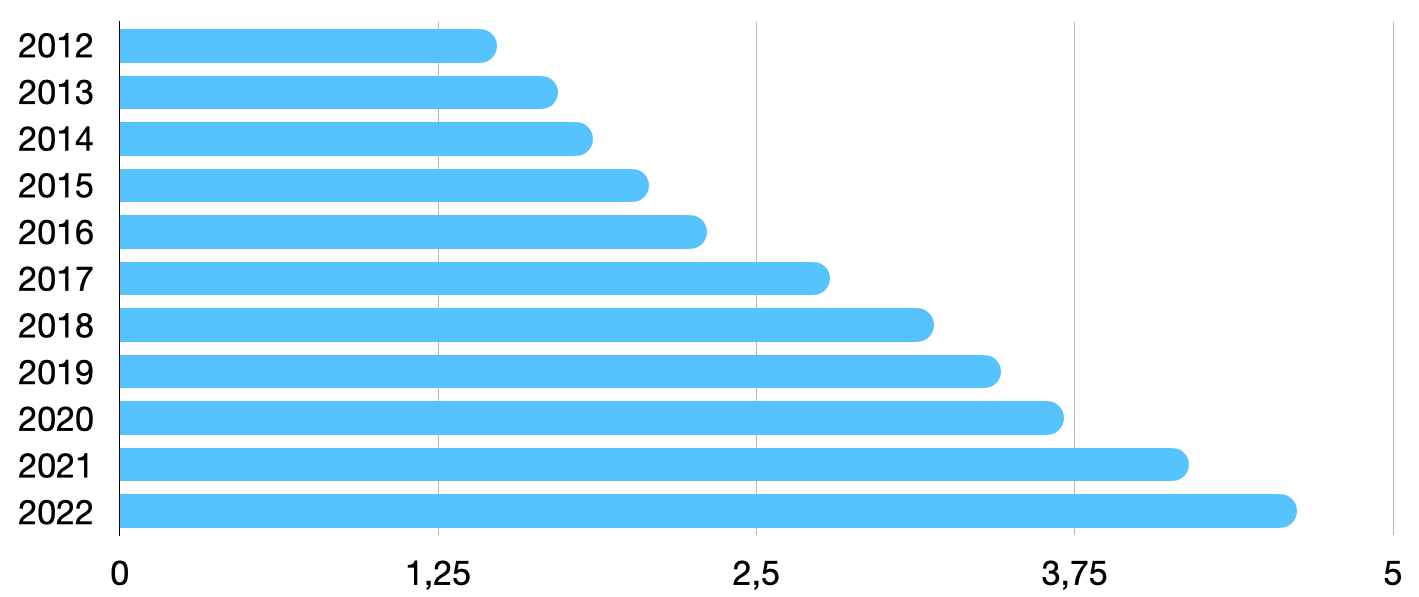
\includegraphics[width=15cm,height=12cm,keepaspectratio]{Immagini/statistiche_social.png}
    \caption{Istogramma a colonne che mostra il numero totale (in miliardi) di utenti utilizzatori di social media a partire da gennaio 2012~\cite{kemp}.}
    \label{fig:social_networks}
\end{figure}

\noindent
L'origine della \textit{social media forensics} è strettamente legata allo sviluppo e alla diffusione dei social network. Fino a poco tempo fa, la maggior parte degli studi condotti in questo ambito è stata eseguita in condizioni controllate e avendo a disposizione informazioni pregresse sul problema analizzato. Solo di recente i ricercatori hanno provato ad estendere questo campo in scenari di vita reale. I risultati ottenuti sono duplici: da un lato si migliora la comprensione del percorso svolto in rete da un oggetto digitale, permettendo di identificare fake news e verificare l'integrità delle informazioni; dall'altro si presentano nuove sfide derivanti dalla possibilità da parte degli utenti di caricare o condividere (anche molteplici volte) immagini e video, comportando un progressivo deterioramento del dato multimediale.\\
Il ciclo di vita di un contenuto digitale è caratterizzato da molteplici fasi~\cite{pasquini2021media}. Ogni step di questo processo lascia tracce distintive che possono essere identificate tramite tecniche differenti. La \textit{social media forensics}, pertanto, può essere suddivisa in tre macro-campi di applicazione: la \textit{forensics analysis}, la \textit{platform provenance analysis} e la \textit{multimodal verification analysis}. Ognuno di questi rami della ricerca risponde a quesiti ben specifici:

\begin{itemize}
    \item \textit{“Quali sono le operazioni compiute su immagini e video durante le fasi di acquisizione e post-processing? Da quale dispositivo provengono?"}
    \item \textit{“Quali sono i social network utilizzati per il caricamento dei contenuti?"}
    \item \textit{“Gli elementi analizzati sono veri oppure falsi? Sono stati inseriti in un contesto sbagliato?"}
\end{itemize}

\subsection{Forensics analysis}
\label{sub_sec:forensics_analysis}

La \textit{forensics analysis} analizza i contenuti digitali per individuare potenziali manomissioni e/o modifiche che minano la credibilità delle informazioni~\cite{bartolucci}. Possiamo riassumere gli obiettivi di questa disciplina in due punti:

\begin{itemize}
    \item Risalire alla fotocamera o al sensore che ha acquisito un determinato oggetto digitale (\textit{source identification});
    \item Verificare che questo oggetto non sia stato alterato tramite operazioni non autorizzate (\textit{integrity verification}).
\end{itemize}

\subsubsection{Source identification}
\label{sub_sub_sec:source_identification}

Con il termine \textit{source identification} ci si riferisce al processo di tracciamento del dispositivo che ha prodotto un particolare contenuto digitale (es., immagine o video). In questo campo i ricercatori hanno analizzato immagini e video con l'obiettivo di trovare risposte a questioni ancora aperte. Nel caso delle immagini sono stati condotti un numero maggiore di lavori data l'ampia disponibilità di dati e la minore complessità del problema. Gestire i video, infatti, è più complicato per via delle dimensioni dei file. I metodi proposti, come spiegato in~\cite{verdoliva}, possono essere suddivisi in due principali categorie: hardware e software. L'approccio hardware studia gli effetti generati dalle lenti o difetti presenti nel sensore durante l'acquisizione, quello software, invece, considera le operazioni di elaborazione compiute dalla camera.\\
Con la nascita dei social network i metodi classici di analisi (es., copy-paste, splicing) sono diventati obsoleti. Le cause principali sono da ricercarsi nelle differenti policy adottate da queste piattaforme. Come risultato, le modifiche apportate nei media digitali dai processi di condivisione e upload/download causano un deterioramento se non una completa cancellazione delle informazioni lasciate dal dispositivo di acquisizione. Gli studi più recenti propongono tecniche basate sul PRNU  (\textit{Photo Response Non-Uniformity})~\cite{bertini2015profile}, sui video file containers~\cite{lopez2020digital} e le \textit{convolutional neural networks}~\cite{rafi2019application}.


\subsubsection{Integrity verification}
\label{sub_sub_sec:integrity_verification}

Se per la \textit{source identification} sono state condotte svariate indagini, lo stesso non si può dire per l'\textit{integrity verification} che per quanto riguarda lo studio di dati provenienti da social network risulta un ramo della disciplina abbastanza inesplorato. Con \textit{integrity verification} si definisce il processo finalizzato alla verifica dell'integrità delle informazioni, tramite l'individuazione di alterazioni causate dall'esecuzione di particolari operazioni.\\
Nell'ambito della \textit{social media forensics}, questa definizione viene applicata ai contenuti digitali che sono stati condivisi tramite diverse piattaforme social e il cui obiettivo è assicurarne la correttezza. Tuttavia, queste verifiche vengono ampiamente ostacolate dalle operazioni compiute da siti web e applicazioni, che possono causare la cancellazione degli indizi su eventuali anomalie. Le poche ricerche condotte in questo ambito hanno impiegato le stesse tecniche utilizzate per le \textit{source identification}. Nel prossimo futuro, lo sviluppo di nuovi metodi potrà offrire ulteriori spunti per la ricerca.


\subsection{Platform provenance analysis}
\label{sub_sec:platform_provenance_analysis}

I social network hanno radicalmente cambiato il mondo, offrendo possibilità che precedentemente non erano nemmeno immaginabili. Se da un lato permettono l'immediata comunicazione tra le persone, dall'altro si contrappongono rischi significativi legati alla sicurezza. Basti pensare al caso in cui, durante un processo, si ha la necessità di individuare l'origine di un file, per risalire all'identità della persona che lo ha diffuso.\\
Il ramo di ricerca della \textit{platform provenance analysis} ha come principale obiettivo quello di ricostruire la storia associata ad un contenuto digitale. È possibile identificare alcuni punti chiave che stanno alla base di questa disciplina:

\begin{itemize}
    \item Risalire alle piattaforme che hanno processato l'oggetto digitale;
    \item Ricostruire l'intera storia di condivisione dell'oggetto digitale;
    \item Estrarre informazioni significative sui sistemi utilizzati nella fase di upload.
\end{itemize}
Per raggiungere tali obiettivi si può analizzare il problema utilizzando metodi di classificazione in cui immagini e video vengono raggruppati basandosi sulla cronologia passata delle condivisioni.\\
Il processo risolutivo (Fig.~\ref{fig:plat_prov_analy}) è il risultato di una serie di fasi sequenziali che prevede come prima operazione l'adozione di un dataset (raccolta di immagini e/o video) che definisca in maniera esaustiva lo scenario affrontato. Possono essere impiegati dataset proprietari generati da zero oppure quelli resi pubblicamente accessibili dalla comunità scientifica. Tra i più importanti troviamo: RAISE~\cite{dang2015raise}, VISION~\cite{shullani2017vision} e UCID~\cite{schaefer2003ucid}.\\
A questo punto, partendo dalle immagini/video presenti nel dataset vengono estratte informazioni rilevanti, o \textit{feature}. Il numero di operazioni che possiamo svolgere su questi dati sono molteplici e distinguibili in due grandi categorie: nella prima troviamo quelle che si concentrano sull'analisi del segnale dell'immagine, mentre nella seconda quelle operazioni che considerano i metadati. Se da un lato l'analisi del segnale permette di ottenere informazioni attraverso lo studio dei pixel per costituire \textit{feature} di tipo statistico (es., istogrammi dei coefficienti DCT), dall'altro i metadati consentono di ricavare in maniera rapida informazioni secondarie (es., tempo e dispositivo di acquisizione e coordinate GPS). Vari approcci includono l'utilizzo combinato dei due sistemi di analisi.\\
La classificazione finale è eseguita tramite l'impiego di algoritmi di \textit{machine learning} adeguatamente allenati con le \textit{feature} estratte nella fase precedente. Gli approcci proposti sono molteplici: si passa dai classici metodi di classificazione supervisionata (es., \textit{support vector machine} o \textit{random forest}) fino ad adottare tecniche di \textit{deep learning}.

\begin{figure}[h!]
    \centering
    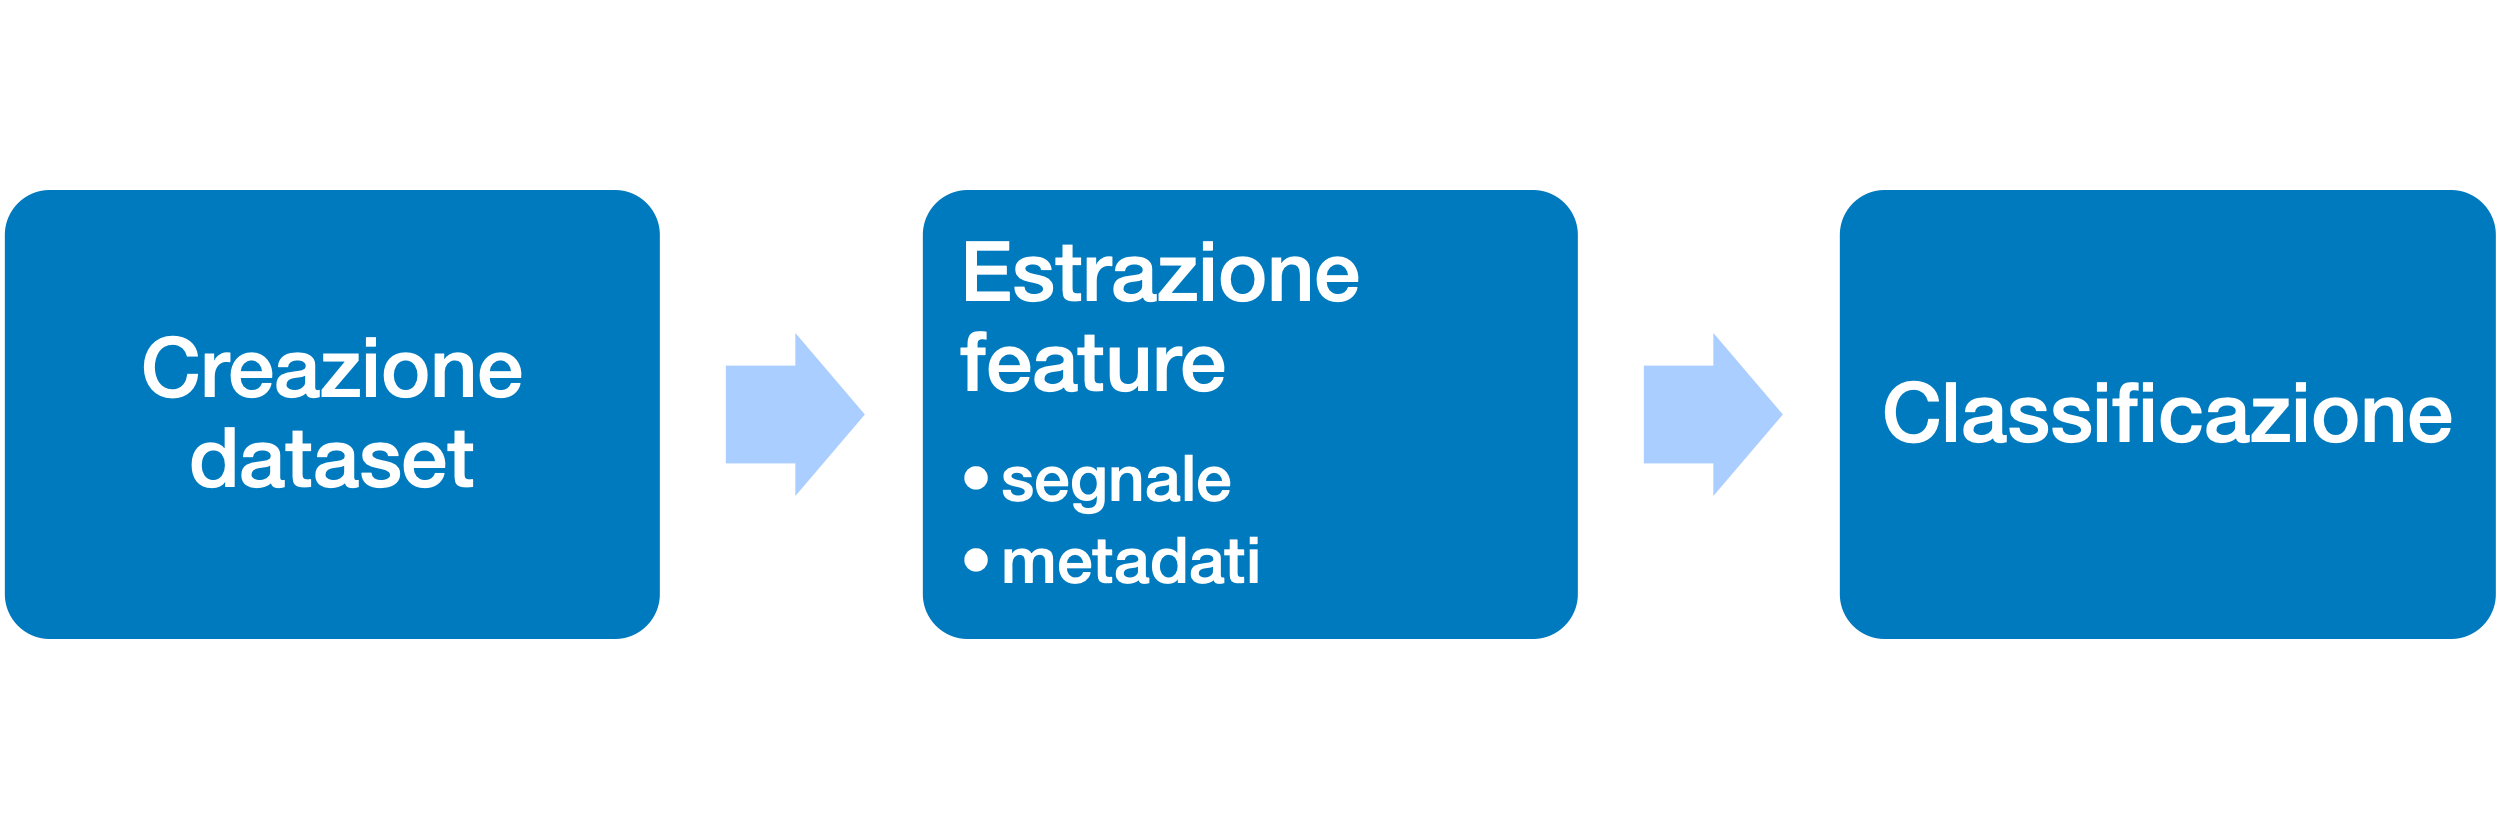
\includegraphics[width=12cm,height=9cm,keepaspectratio]{Immagini/platform_provenance_analysis.png}
    \caption{Processo seguito per la \textit{platform provenance analysis}.}
    \label{fig:plat_prov_analy}
\end{figure}

\subsection{Multimodal verification analysis}
\label{sub_sec:multimodal_verification_analysis}

La costante crescita di popolarità delle piattaforme digitali ha determinato un cambiamento del modo in cui le persone ricercano e ricevono informazioni. Se fino a non molto tempo fa telegiornali, riviste e notiziari erano la principale fonte di comunicazione, adesso lo scenario è cambiato: annunci e notizie dal mondo vengono raccolte e diffuse da blog, forum e applicazioni proprietarie. La velocità di diffusione delle informazioni ha eliminato ogni confine ma, al tempo stesso, la possibilità che vengano manipolate o addirittura create ad hoc rappresenta uno scenario preoccupante. Campagne politiche, fake news, attacchi terroristici, teorie cospirazioniste, come anche notizie vere ma decontestualizzate, necessitano di sistemi di regolazione.\\
Il ramo di ricerca della \textit{multimodal verification analysis} studia i metodi utilizzati per diffondere disinformazione con due principali scopi: scovare eventuali modifiche delle informazioni diffuse e identificare qualora una notizia vera sia stata volutamente associata all'interno di un contesto sbagliato. Così come avviene nella \textit{platform provenance analysis}, anche la \textit{multimodal verification analysis} dedica particolare attenzione all'analisi delle operazioni veicolate tramite i social network. Le condivisioni sulle diverse piattaforme (es., Twitter, Instagram, Facebook) hanno strutture differenti in base al tipo di post utilizzato: solo testo, immagini/video oppure una combinazione dei due.\\
L'analisi prende in considerazione tre tipologie di elementi:

\begin{itemize}
    \item Informazioni visive ricavate da immagini o video associati agli oggetti digitali condivisi;
    \item Informazioni testuali derivate dal testo associato ai post pubblicati;
    \item Metadati ricavati dalla combinazione di due fattori: quelli strettamente legati al contenuto digitale condiviso e quelli che prendono in considerazione l'utente che ha diffuso le informazioni (es., numero di commenti, numero di follower, frequenza di pubblicazione, etc.)
\end{itemize}
In conclusione, il dominio di applicazione della \textit{social media forensics} è rappresentato dalla \textit{forensics analysis}, dalla \textit{platform provenance analysis} e dalla \textit{multimodal verification analysis} (Fig.~\ref{fig:mappa}). I metodi e le soluzioni fornite da queste discipline non sono unicamente ristretti alla pura ricerca, ma possono offrire un contributo attivo nella fase di investigazione.

\section{Obiettivi}
\label{sec:obiettivi}

Il lavoro proposto in questa tesi rientra nell'ambito della \textit{platform provenance analysis}, ma propone un aspetto nuovo e fino ad ora inesplorato. La maggior parte dei lavori svolti in questo campo tende a considerare molteplici piattaforme di condivisione, cercando di ricostruire la catena di social in cui un contenuto digitale è stato diffuso. Nel nostro caso, invece, consideriamo un solo social network, WhatsApp, ma cerchiamo di risalire al tipo di device e al sistema operativo utilizzato per l'upload. Nei prossimi capitoli forniremo un'analisi dei lavori più rilevanti svolti nel campo della \textit{platform provenance analysis}, dopodiché mostreremo l'approccio da noi adottato e i risultati finali ottenuti.

\begin{figure}[h!]
    \centering
    \adjustbox{scale=0.45}{
    \begin{tikzpicture}[
        mindmap,
        grow cyclic, text width=4cm, align=flush center,
        every node/.style={concept, font=\fontsize{6mm}{6mm}\selectfont},
        concept color=orange!40,
        level 1/.style={level distance=9.2cm, sibling angle=120},
        level 2/.style={level distance=6.2cm, sibling angle=60}
    ]
    
    \node [root concept, scale=2] {\textbf{Social media forensics}}
        child [concept color=blue!30] {node {\textbf{Forensics analysis}}
            child {node {Identificazione sorgente}}
            child {node {Verifica integrità}}
        }
        child [concept color=teal!40] {node {\textbf{Platform provenance analysis}}
            child {node {Identificazione piattaforme di condivisione}}
            child {node {Ricostruzione storia oggetto digitale}}
            child {node {Estrazione informazioni dai sistemi di upload}}
        }
        child [concept color=yellow!30] {node {\textbf{Multimodal verification analysis}}
            child {node {Verifica credibilità dei contenuti}}
            child {node {Identificazione informazioni false}}
            child {node {Individuazione dati sintetici}}
        };
    \end{tikzpicture}
    }
    \caption{Le tre macro-categorie che compongono la \textit{social media forensics}.}
    \label{fig:mappa}
\end{figure}



      \chapter{Platform provenance: stato dell'arte}
\label{cha:ppa}
In questo capitolo viene presentata una descrizione dei metodi che rappresentano lo stato dell'arte della \textit{platform provenance analysis} (PPA), prendendo in considerazione i principali lavori proposti in letteratura. Si partirà dall'esaminare una serie di dataset creati dalla comunità scientifica (\ref{sec:dataset}), mettendo in evidenza le caratteristiche e differenze. A seguire verranno presentate le tecniche adottate per l'estrazione di \textit{feature} (\ref{sec:feature}), specificandone l'origine e le possibilità di utilizzo. Saranno poi elencati gli algoritmi di classificazione (\ref{sec:ml_model}), sia quelli già noti che quelli sviluppati ad hoc, e successivamente raggruppati in diverse categorie in base al loro funzionamento. Infine, come conclusione al capitolo, discuteremo i problemi aperti e i possibili sviluppi futuri di questo campo (\ref{sec:cosa_rimane_da_fare}).

\section{Dataset}
\label{sec:dataset}
La realizzazione di un dataset è particolarmente delicata e significativa poiché consente di raccogliere i dati necessari per studiare ed approcciare il problema. Nell'ambito della PPA, si tratta tipicamente di raccolte di immagini e/o video, condivisi tramite uno o più dispositivi e su uno o più social network. Ogni database presenta poi caratteristiche differenti in base al tipo di uso per cui sono stati pensati. Nel caso delle immagini vengono utilizzati differenti formati (es., JPEG, RAW), risoluzioni, livelli di compressione, oltre che un'ampia varietà di soggetti e scene raffigurate. Per quanto riguarda i video, invece, sono stati creati un numero inferiore di dataset a causa delle problematiche legate alla gestione di una mole di dati molto più grande.\\
Il processo di composizione di un dataset può essere riassunto in cinque punti fondamentali: selezione delle immagini di partenza; selezione dei dispositivi (es., smartphone, tablet, computer) da cui condividere le immagini; scelta delle piattaforme social su cui caricare i contenuti; download delle immagini condivise; organizzazione dei dati ottenuti. Di seguito vengono illustrati i principali dataset che possono essere impiegati per la PPA, con le relative caratteristiche.

\begin{itemize}
    \item \textit{VISION} \cite{shullani2017vision}: creato per \textit{l'image source identification} (ISI) e per la \textit{video source identification} (VSI), comprende oltre 34000 immagini e 1900 video provenienti da 35 modelli di smartphone e tablet di 11 diversi brand (es., Apple, Lenovo, Microsoft, Samsung, Sony, etc.). Le immagini sono state condivise in alta e bassa qualità su Facebook e WhatsApp; i video sono stati caricati con la massima risoluzione possibile su WhatsApp e YouTube. I sistemi operativi presi in considerazione sono iOS (dalla versione 7 alla 10), Android (dalla versione 6 alla 7) e Windows Phone OS 8.1.
    
    \item \textit{V-SMUD} \cite{phan2019tracking}: acronimo di \textit{VISION Social Multiple Up-Download}, è formato da 510 immagini JPEG provenienti dal dataset VISION e condivise fino a 3 volte utilizzando tre piattaforme differenti: Facebook, Flickr e Twitter. Le $510\times39 = 19890$ immagini ottenute vanno a comporre il dataset finale.
    
    \item \textit{RAISE} \cite{dang2015raise}: realizzato per l'\textit{image forensics}, questo dataset comprende 8156 immagini in formato originale RAW catturate tramite l'utilizzo di tre diverse macchine fotografiche (Nikon D40, Nikon D90 e Nikon D7000). Le immagini sono state salvate a tre diverse risoluzioni: $3008\times2000$, $4288\times2848$ e $4928\times3264$ pixel. Ognuna di esse è stata poi classificata in una o più delle seguenti categorie: \textit{“outdoor"}, \textit{“indoor"}, \textit{“landscape"}, \textit{“nature"}, \textit{“people"}, \textit{“objects"} e \textit{“buildings"}. RAISE è stato creato con due scopi principali: mettere a disposizione della comunità scientifica un ampio database di immagini per uso forense ed eliminare il problema della privacy legato all'utilizzo di contenuti scaricati dal web. Per facilitare l'utilizzo di RAISE, gli autori hanno anche reso pubblici sottoinsiemi di questo dataset contenenti un numero di elementi pari a 1000 (RAISE-1K), 2000 (RAISE-2K), 4000 (RAISE-4K) e 6000 (RAISE-6K).
    
    \item \textit{R-SMUD} \cite{phan2019tracking}: come V-SMUD, R-SMUD è stato creato a partire da immagini che fanno parte di un altro dataset, in questo caso RAISE. È costituito da 900 immagini con tre risoluzioni differenti ($337\times600$, $1012\times1800$, $1687\times3000$), con un aspect-ratio di $9:16$ e compresse nel formato JPEG in 6 \textit{quality factor} diversi ($QF = 50, 60, 70, 80, 90, 100$). Ogni elemento di R-SMUD è stato in seguito condiviso attraverso tre social network (Facebook, Flickr e Twitter) ottenendo in questo modo 35100 immagini.
    
    \item \textit{SDRG} \cite{rouhi2021no}: dataset costruito con gli obiettivi di identificare il dispositivo che ha effettuato la condivisione (\textit{smartphone identification}) e associare tramite le informazioni a disposizione il corrispondente profilo utente (\textit{user profile linking}). SDRG comprende 4500 immagini, con diverse risoluzioni ottenute da smartphone di 18 brand (es., Apple, LG, Motorola, Nokia, etc.) e successivamente caricate su 4 social network: Facebook, Google Currents, Telegram e WhatsApp.
    
    \item \textit{ISIMA} \cite{Phan2018}: raccoglie immagini condivise su applicazioni di messaggistica istantanea, prendendo in considerazione Facebook Messenger, Telegram e WhatsApp. Queste immagini (in formato JPEG) sono state caricate utilizzando due tipologie di smartphone, ovvero Android e Apple. Le immagini contenute in questo dataset possono essere raggruppate in due categorie: \textit{single-shared}, ovvero condivise una sola volta e \textit{double-shared}, condivise una seconda volta, per un totale di 8400 elementi.
    
    \item \textit{FODB} \cite{hadwiger2021forchheim}: rappresenta il dataset più recente tra quelli menzionati e si pone l'obiettivo di separare il contenuto di un'immagine dalle relative tracce forensi, e mettere a disposizione uno strumento per analizzare le operazioni di compressione effettuate dai social network. La sua realizzazione è avvenuta attraverso l'utilizzo di 25 diversi modelli di smartphone, appartenenti a 9 brand. I social media adottati per la condivisione sono: Facebook, Instagram, Telegram, Twitter e WhatsApp.
    
\end{itemize}
La tabella \ref{tab:lista_dataset} riporta una sintesi delle principali caratteristiche dei dataset presentati. 

\begin{center}
    \begin{adjustbox}{max width=\textwidth}
    \begin{tabular}{ccccccc}
        \hline
        \\[-1em]
        \textbf{Dataset} & \textbf{Immagini} & \textbf{Video} & \textbf{N. immagini} & \textbf{N. video} & \textbf{Brand} & \textbf{Social network}\\[-1em]\\
        \hline
        \\
        VISION & \ding{51} & \ding{51} & 34427 & 1914 & \parbox{5cm}{Apple, Asus, Huawei, Lenovo, LG, Microsoft, OnePlus, Samsung, Sony, Wiko, Xiaomi} & \parbox{5cm}{Facebook, WhatsApp, YouTube}\\\\
        \\
        V-SMUD & \ding{51} & \ding{55} & 19890 & - & \parbox{5cm}{Apple, Asus, Huawei, Lenovo, LG, Microsoft, OnePlus, Samsung, Sony, Wiko, Xiaomi} & \parbox{5cm}{Facebook, Flickr, Twitter}\\\\
        \\
        RAISE & \ding{51} & \ding{55} & 8156 & - & \parbox{5cm}{Nikon} & \parbox{5cm}{ \begin{center} - \end{center} }\\\\
        \\
        R-SMUD & \ding{51} & \ding{55} & 35100 & - & \parbox{5cm}{ \begin{center} - \end{center}} & \parbox{5cm}{Facebook, Flickr, Twitter}\\\\
        \\
        SDRG & \ding{51} & \ding{55} & 4500 & - & \parbox{5cm}{Apple, HTC, Huawei, LG, Motorola, Nokia, Samsung, Sony} & \parbox{5cm}{Facebook, Google Currents, Telegram, WhatsApp}\\\\
        \\
        ISIMA & \ding{51} & \ding{55} & 9100 & - & \parbox{5cm}{Apple, Asus, Huawei, Lenovo, LG, Microsoft, OnePlus, Samsung, Sony, Wiko, Xiaomi} & \parbox{5cm}{Facebook Messenger, Telegram, WhatsApp}\\\\
        \\
        FODB & \ding{51} & \ding{55} & 23106 & - & \parbox{5cm}{Apple, BQ, Google, Huawei, LG, Motorola, Samsung, Sony, Wiko} & \parbox{5cm}{Facebook, Instagram, Telegram, Twitter, WhatsApp}\\\\
        \bottomrule
    \end{tabular}
    \end{adjustbox}
\end{center}
\captionof{table}{\label{tab:lista_dataset}Da sinistra a destra sono riportati: il nome, la presenza di immagini e/o video tramite i simboli \ding{51} e \ding{55}; il numero di immagini/video presenti; i brand dei dispositivi considerati; le piattaforme social utilizzate~\cite{pasquini2021media}.}

\section{Estrazione feature}
\label{sec:feature}
Partendo dai dati raccolti nella fase precedente, si passa alla fase di estrazione di \textit{feature}. Queste sono ricavate in modo tale da analizzare le operazioni subite dai media digitali durante la condivisione e le fasi di upload/download. Infatti, i processi a cui vengono sottoposti i contenuti multimediali contribuiscono a modificarli lasciando tracce distintive. Queste modifiche, nella maggior parte dei casi, sono univoche e rappresentano indizi importanti per ricostruire la storia di un contenuto digitale.\\
Come menzionato nel capitolo introduttivo, le \textit{feature} possono essere ricavate in due modi: a partire dall'analisi del segnale oppure attraverso i metadati. Nel primo caso viene analizzato il cambiamento avvenuto nei pixel dell'immagine dopo la condivisione; nel secondo, si cercano eventuali modifiche apportate dalle piattaforme sulle strutture dati degli oggetti digitali. Queste \textit{feature} vengono infine raggruppate sotto forma di vettori numerici. Gli studi condotti nel campo della PPA hanno anche sviluppato tecniche che fondono assieme segnale e metadati, per creare metodi ibridi.\\
Verranno ora presentate alcune tecniche che utilizzano \textit{feature} basate sull'analisi del segnale. In letteratura scientifica sono stati proposti nel tempo molteplici approcci. Per esempio, in~\cite{moltisanti2015image} vengono esaminate le modifiche apportate sulle immagini dall'algoritmo utilizzato da Facebook al fine di identificarne le operazioni svolte. Gli aspetti su cui è stata posta particolare attenzione sono due: come le immagini vengono ridimensionate a seguito del caricamento e in che modo queste sono compresse. Dai risultati ottenuti è emerso che un'immagine pubblicata tramite Facebook viene ridimensionata solo in alcune circostanze, in particolare sulla base del numero di pixel nel lato più lungo dell'immagine e dell'attivazione o meno dell'opzione di caricamento in alta qualità.\\
Sempre nell'ambito dell'analisi del segnale un aiuto significativo è rappresentato da \textit{feature} di tipo statistico, come per esempio gli istogrammi dei coefficienti DCT (\textit{Discrete Cosine Transform}). La costruzione di tali elementi avviene suddividendo l'immagine di partenza in un determinato numero di blocchi, di dimensione fissata, per ognuno dei quali si calcolano i relativi coefficienti DCT. Infine, gli istogrammi dei coefficienti vanno a costituire il vettore di \textit{feature}. Molteplici studi seguono questa strada~\cite{caldelli2017image, amerini2017tracing, amerini2019social} perché le tracce lasciate nelle immagini non possono essere eliminate, a differenza dei metadati facilmente rimovibili. In~\cite{amerini2019social}, oltre a considerare \textit{feature} basate sui coefficienti DCT, ne vengono estratte anche di relative al rumore introdotto nelle immagini dai social network.\\
Esistono poi una serie di lavori che utilizzano i metadati come principale fonte di informazioni. Un esempio è dato da~\cite{mullan2019forensic} che, attraverso un'analisi dei metadati, ha permesso di risalire ai dispositivi (smartphone Apple) utilizzati per la condivisione delle immagini. Obiettivo principale di questo studio era dimostrare che i soli metadati sono sufficienti a identificare con elevata precisione le diverse versioni software impiegate da questi dispositivi. Sono stati utilizzati i dati EXIF (\textit{Exchangeable Image File Format}, uno standard che codifica specifiche informazioni associate ad un'immagine, quali i valori di scatto, la data e l'ora di acquisizione \cite{nasim}) e i parametri dell'algoritmo di codifica JPEG. In~\cite{mullan2019forensic}, è stato mostrato come sia possibile suddividere tali informazioni in due categorie: \textit{“camera data"} e \textit{“other data"}. Nonostante i metadati rappresentino un'importante fonte di informazioni, in alcuni casi vengono rimossi dai social media nel momento in cui si effettua l'upload. Di conseguenza il loro utilizzo non rappresenta sempre una via percorribile.\\
Infine, sono stati sviluppati una serie di metodi che sfruttano in combinazione \textit{feature} derivate dal segnale e dai metadati. Se da un lato per questi approcci si riscontrano difficoltà nel modo di unire i due tipi di \textit{feature}, la loro fusione permette di sfruttare i punti di forza di entrambe. A tal proposito,~\cite{phan2018identifying} adotta un approccio basato sulla fusione di \textit{feature} per applicazioni di messaggistica istantanea, mentre \cite{verde2021multi} si concentra sui social network. Le \textit{feature} utilizzate nel primo caso sono il risultato della composizione di istogrammi DCT (369) e metadati (152) estratte dalle immagini, per un totale di 521 elementi. In~\cite{verde2021multi} ne viene presentato anche un terzo insieme chiamato HEADER che contiene informazioni ricavate dall'header JPEG delle immagini.

\section{Modelli di machine learning}
\label{sec:ml_model}
Il passo successivo della PPA è rappresentato dalla classificazione automatica, tramite la quale i dati a disposizione vengono suddivisi in cluster, ad ognuno dei quali è associata un'etichetta, o \textit{label}. Per effettuare questa operazione vengono tipicamente utilizzati algoritmi di \textit{machine learning}, che apprendono automaticamente il criterio ottimo di separazione delle \textit{feature} estratte. Ad oggi possiamo suddividere i lavori proposti in due principali categorie: quelli che adottato classici metodi di classificazione supervisionata e quelli che utilizzano metodi basati sul \textit{deep learning}. Nel primo caso, gli algoritmi più utilizzati sono \textit{random forest}~\cite{phan2018identifying, mullan2019forensic, caldelli2017image, verde2021multi}, \textit{decision tree}~\cite{giudice2017classification} e \textit{support vector machine}~\cite{phan2018identifying}. Per quanto riguarda il \textit{deep learning}, i metodi più utilizzati si basano sulle \textit{convolutional neural network} (CNN)~\cite{amerini2019social, amerini2017tracing, phan2019tracking}. Queste ultime stanno assumendo sempre più importanza data la possibilità di apprendere automaticamente le \textit{feature} più rappresentative direttamente dai dati e le elevate performance ottenibili.

\section{Problemi aperti}
\label{sec:cosa_rimane_da_fare}
Nonostante i progressi effettuati nel campo della PPA, vi sono ancora una serie di domande aperte. Innanzitutto, la maggior parte delle tecniche presentate si concentra sulle immagini. Esse costituiscono un dominio di studio più semplice rispetto ai video, per le ragioni già citate. Come riportato in~\cite{pasquini2021media}, tutti i metodi sviluppati sino a questo momento utilizzano approcci induttivi piuttosto che deduttivi a causa dell'assenza di procedimenti standard per eseguire le operazioni. Per esempio, l'affidabilità delle tecniche adottate (in termini di performance) è fortemente dipendente dalla qualità dei dati prodotti, e dunque lo sviluppo di nuovi metodi può risultare difficile nel momento in cui le informazioni a disposizione non sono sufficienti o adeguate. I lavori effettuati nell'ambito della PPA tendono a considerare più social network per ricostruire la catena di condivisioni, non ponendo particolare attenzione al riconoscimento del dispositivo o sistema adottato per il caricamento dei media digitali. Questo ultimo elemento è oggetto di discussione del prossimo capitolo.



      \chapter{Metodo proposto}
\label{cha:metodo_proposto}

Nel terzo capitolo viene presentata la metodologia seguita per l'analisi di immagini condivise tramite la piattaforma WhatsApp con l'obiettivo di risalire al dispositivo e al sistema software impiegato (Fig.~\ref{fig:metodo}). Come prima cosa sarà descritto il modo in cui è stato creato SHADE, dataset appositamente realizzato per questo scopo (\ref{sec:SHADE}). In seguito esamineremo due metriche, \textit{Mean Square Error} (MSE) e \textit{Peak Signal-to-Noise Ratio} (PSNR), utilizzate per un'analisi di tipo qualitativo delle immagini (\ref{sec:mse_psnr}). Si passerà poi a descrivere la fase di estrazione di \textit{feature} (\ref{sec:estr_feat}) e la loro visualizzazione grazie alla creazione di mappe Isomap (\ref{sub:isomap}). Come ultimo passaggio, illustreremo i due metodi utilizzati per la classificazione (\ref{sec:classificazione}). Tutte le fasi qui riportate sono state accompagnate dalla scrittura di codice Python per l'analisi, la visualizzazione e la classificazione delle immagini.

\begin{figure}[h!]
    \centering
    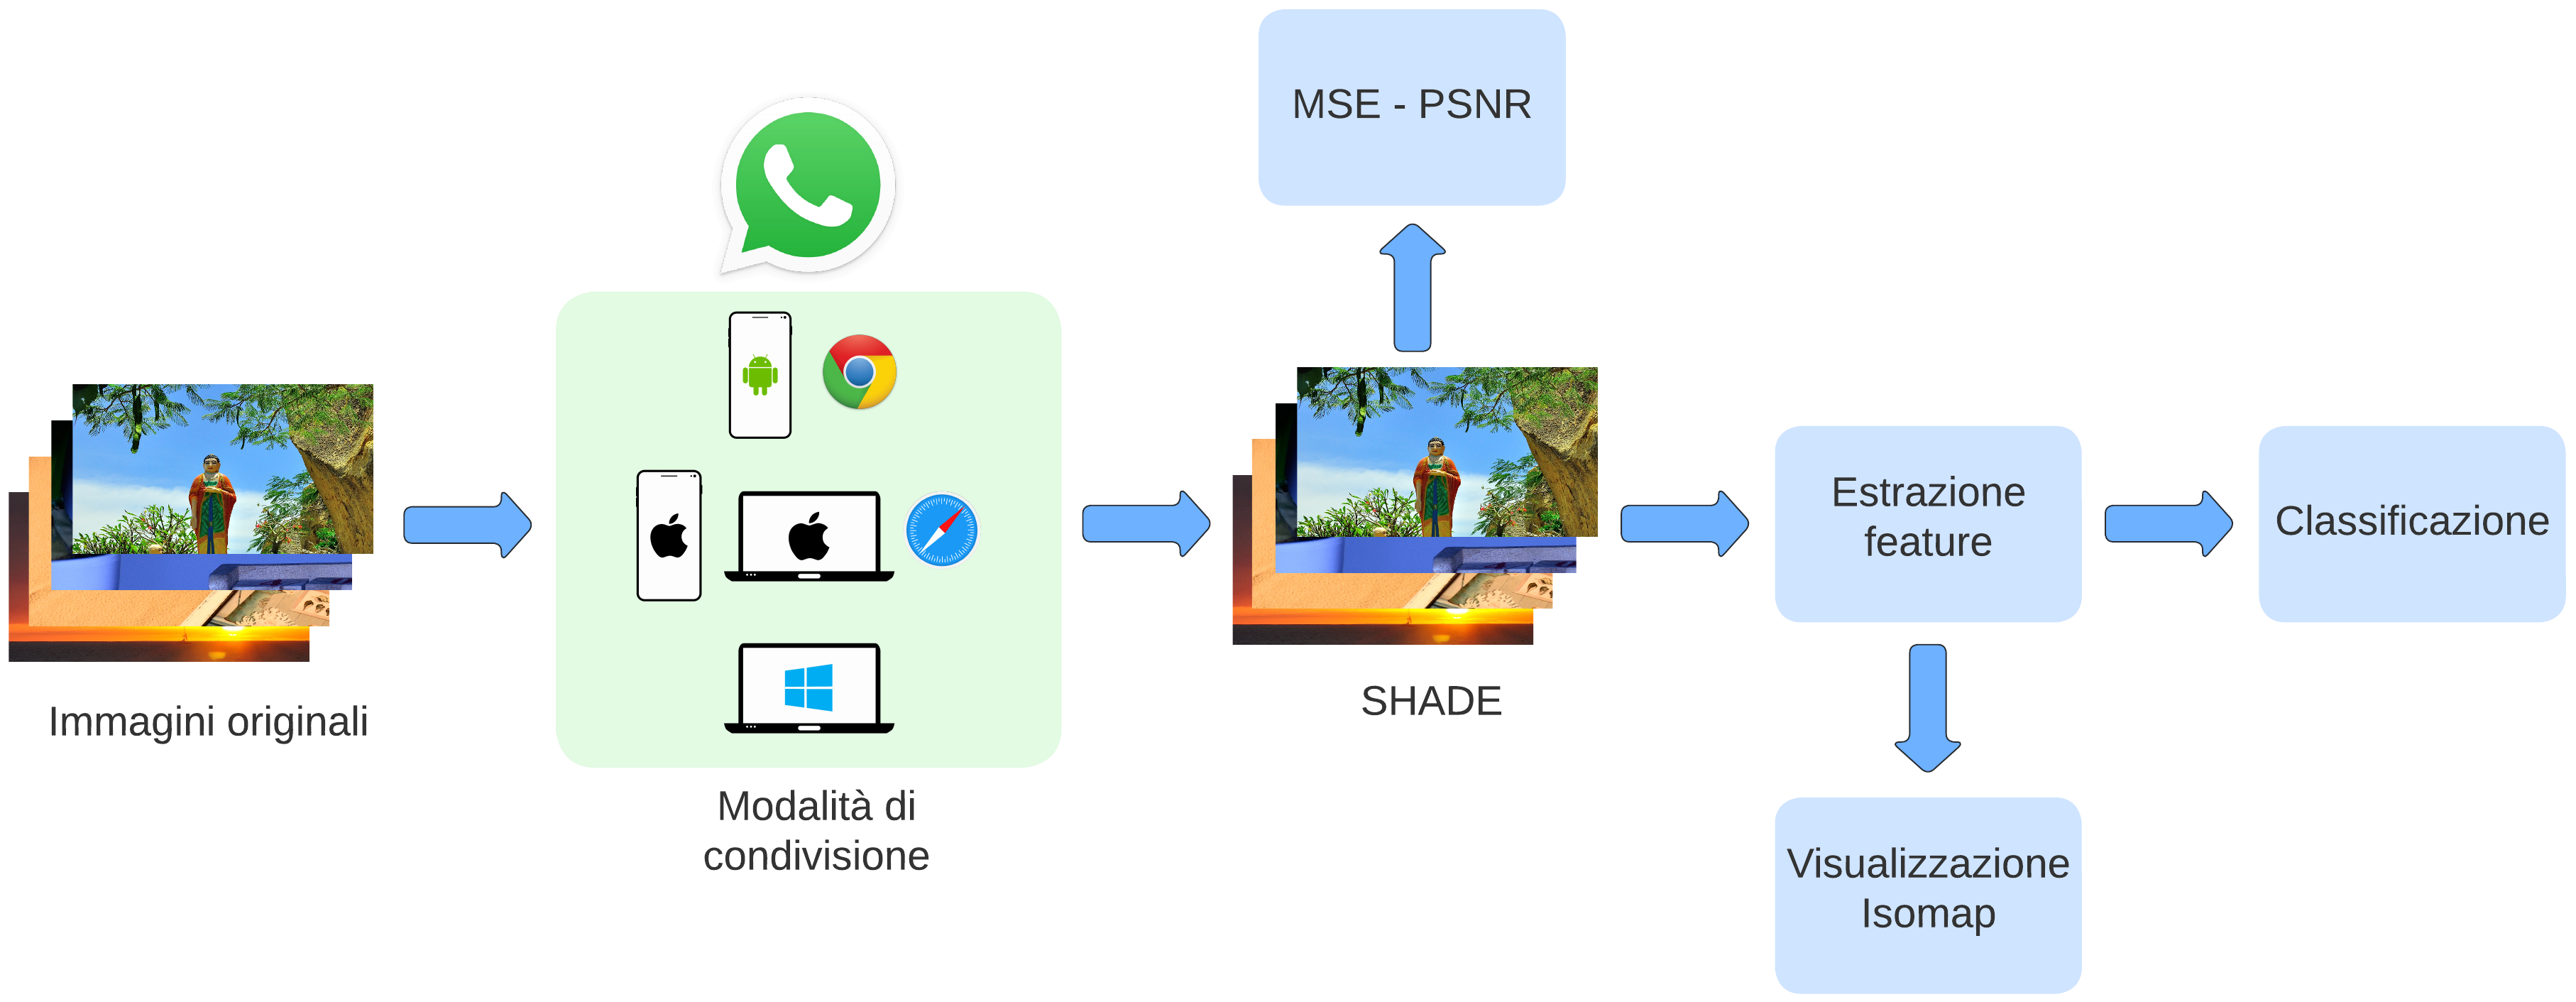
\includegraphics[width=\columnwidth]{Immagini/metodo_proposto.png}
    \caption{\textit{Pipeline} seguita per le analisi su SHADE}
    \label{fig:metodo}
\end{figure}

\section{SHADE}
\label{sec:SHADE}

Il processo di creazione di SHADE (acronimo di \textit{SHAring DEvice}) è partito da 50 immagini in formato RAW prese dal dataset RAISE. In maniera simile a quanto avvenuto per R-SMUD le immagini sono state ritagliate dall'angolo sinistro superiore per ottenere tre copie con le seguenti risoluzioni: $337\times600$, $1012\times1800$ e $1687\times3000$ con un \textit{aspect ratio} di $9:16$. Tutte le immagini ritagliate hanno poi subito una compressione JPEG utilizzando sei \textit{quality factor} differenti (QF = 50, 60, 70, 80, 90, 100) per un totale di 900 elementi ($50\times3\times6$).
La piattaforma social che abbiamo selezionato per la condivisione è WhatsApp ed è stata scelta per una serie di motivazioni: rappresenta uno dei più famosi social network per lo scambio di informazioni e mette a disposizione molteplici interfacce software (desktop, browser, mobile) per diversi sistemi operativi (Windows, Android, iOS) permettendo di studiarne i numerosi aspetti del suo funzionamento. Le modalità di condivisione prese in esame sono:\newpage

\begin{table}[h!]
    \normalsize
    \centering
    \begin{tabular}{ll}
        \textbf{Tag} & \textbf{Descrizione}\\
        \midrule
        \textit{ANDROID} & Applicazione mobile per Android\\
        \textit{APP-MAC} & Applicazione desktop per MacOS\\
        \textit{APP-WIN} & Applicazione desktop per Windows 10\\
        \textit{IPHONE} & Applicazione mobile per iOS\\
        \textit{WEB-IPAD} & Browser (Safari) per iPadOS\\
        \textit{WEB-MAC} & Browser (Safari) per MacOS\\
        \textit{WEB-WIN} & Browser (Chrome) per Windows 10\\
    \end{tabular}
\end{table}

Ognuna delle 150 immagini di partenza è stata condivisa sette volte attraverso i metodi sopra elencati e, per ogni \textit{quality factor}, altre sei volte. In questo modo il dataset finale è costituito da $150\times6\times7 = 6300$ elementi a cui si aggiungono le 900 immagini originali non condivise. 
Come nella fase di upload anche il download dei contenuti da WhatsApp è stato eseguito manualmente a causa della mancanza di API (\textit{Application Programming Interface}) gratuite che avrebbero permesso di gestire con maggiore facilità le immagini.  Durante il salvataggio queste vengono rinominate da WhatsApp con un pattern distintivo. Nel nome del file è possibile identificare quattro elementi riportati di seguito con un esempio:

\begin{equation}
    \underbrace{\vphantom{.jpeg} WhatsApp \ \ Image}_{nome} \ \ \underbrace{\vphantom{.jpeg}2021-12-09}_{data} \ \ at \ \ \underbrace{\vphantom{.jpeg}17.38.02}_{ora} \ \ \underbrace{.jpeg}_{formato}
\end{equation}

Per mantenere coerenza con i nomi dei file non condivisi, tutte le immagini scaricate sono state rinominate come \texttt{original-[id]-[h]x[w].jpeg}, dove \texttt{id} corrisponde all'identificatore della relativa immagine originale mentre \texttt{h} e \texttt{w} indicano la risoluzione espressa come prodotto tra altezza e larghezza. Come ultima operazione tutti gli elementi di SHADE sono stati organizzati nel modo seguente: abbiamo dapprima suddiviso le immagini discriminando per la modalità di condivisione creando sette sotto-cartelle più una contenente i file originali. All'interno di ogni directory le immagini sono state ulteriormente suddivise in base al \textit{quality factor} utilizzato per la compressione JPEG. Il seguente albero schematizza la struttura finale del dataset.

\begin{center}
    \begin{adjustbox}{max width=\textwidth, totalheight={11cm}, keepaspectratio}
    \begin{forest}
      pic dir tree,
      where level=0{}{
        directory,
      },
      [/
        [ANDROID
          [QF-50
            [immagine.jpeg, file
            ]
          ]
          [QF-60
          ]
          [QF-70
          ]
          [QF-80
          ]
          [QF-90
          ]
          [QF-100
          ]
        ]
        [APP-MAC
        ]
        [APP-WIN
        ]
        [IPHONE
        ]
        [original
        ]
        [WEB-IPAD
        ]
        [WEB-MAC
        ]
        [WEB-WIN
        ]
      ]
    \end{forest}
    \end{adjustbox}
\end{center}

SHADE è stato presentato in~\cite{tomasoni2022device} ed è pubblicamente accessibile e scaricabile al seguente link: \url{https://mmlab.disi.unitn.it/resources/published-datasets}.

\section{Calcolo MSE e PSNR}
\label{sec:mse_psnr}

Prima di procedere con l'estrazione delle \textit{feature} è stato effettuato un passo intermedio attraverso il calcolo del \textit{Mean Square Error} e del \textit{Peak Signal-to-Noise Ratio}. Queste due metriche analizzano i valori dei pixel dell'immagine e possono essere utilizzate per confrontare la qualità della compressione a cui due oggetti sono stati sottoposti. L'MSE, in particolare, rappresenta l'errore quadratico cumulativo e tanto più è alto questo valore maggiore è la differenza che esiste tra le due immagini considerate. Il PSNR, invece, può essere calcolato a partire dall'MSE e misura l'indice di qualità della compressione che è stata applicata. Più il valore è elevato maggiore è la qualità della prima immagine rispetto alla seconda. Nel nostro caso li abbiamo utilizzati entrambi per verificare se i diversi metodi di condivisione applicano procedure diverse, non solo tra i vari sistemi operativi ma anche nel caso delle singole modalità. Quello che abbiamo fatto è stato calcolare il MSE e il PSNR per ogni coppia di immagini. I valori ottenuti sono stati poi rappresentati utilizzando dei \textit{boxplot} e i dettagli relativi ai risultati si trovano nella sezione~\ref{sec:mse_psnr_results}. I due frammenti di codice Python che seguono mostrano come sono state calcolate queste metriche.

\begin{center}
\rule{9cm}{0.5pt}
\end{center}
\lstinputlisting[language=Python, firstline=1, lastline=19]{File/file_supporto.py}
\begin{center}
\rule{9cm}{0.5pt}
\end{center}
La funzione \textit{MSE()} prende in input \textit{image\textunderscore 1} e \textit{image\textunderscore 2} di cui si vuole trovare il \textit{Mean Square Error}. Possiamo identificare al suo interno tre sezioni distinte. Nella prima vengono create quattro variabili (\textit{height\textunderscore 1}, \textit{width\textunderscore 1}, \textit{height\textunderscore 2}, \textit{width\textunderscore 2}) che contengono rispettivamente altezza e larghezza delle due immagini. Nella seconda troviamo una condizione che effettua il seguente controllo: se la risoluzione delle due immagini non corrisponde allora non è possibile ricavare il MSE e l'esecuzione viene interrotta. Nel caso in cui siano uguali il valore viene calcolato sfruttando la funzione \textit{mean()} del modulo Numpy~\cite{numpy}.\newpage

\begin{center}
\rule{9cm}{0.5pt}
\end{center}
\lstinputlisting[language=Python, firstline=21, lastline=35]{File/file_supporto.py}
\begin{center}
\rule{9cm}{0.5pt}
\end{center}

Il calcolo del PSNR parte dal valore del MSE ricavato in precedenza. Il costrutto \textit{if-else} della funzione \textit{PSNR()} determina le azioni da svolgere: se il valore della variabile \textit{mse} è diverso da \textit{0} allora è possibile calcolare il \textit{Peak Signal-to-Noise Ratio} mentre se la condizione non è soddisfatta viene restituito \textit{NaN} poiché non sarebbe possibile eseguire la divisione. La variabile \textit{max\textunderscore pixel}, necessaria per il calcolo, contiene il valore massimo assumibile dai pixel delle immagini. Per ricavare questo valore sono state utilizzate le funzioni \textit{log10()} e \textit{sqrt()} importate dalla libreria \textit{math} di Python.

\section{Feature}
\label{sec:estr_feat}

Per poter classificare le immagini contenute in SHADE abbiamo necessità di estrarre informazioni rilevanti dal punto di vista forense attraverso l'utilizzo dei cosiddetti \textit{feature descriptors}. Alcuni lavori svolti nell'ambito della \textit{platform provenance analysis} hanno dimostrato l'utilità di descrittori eterogenei al fine di identificare le tracce lasciate dalle piattaforme di condivisione. Abbiamo deciso di seguire la stessa strada di~\cite{verde2021multi} sfruttando un insieme di \textit{feature} relativo ai coefficienti DCT, ai metadati e alle informazioni codificate nell'header JPEG delle immagini.

\begin{itemize}
    \item \textit{DCT}: queste \textit{feature} codificano informazioni legate ai metodi utilizzati per la compressione JPEG. La loro estrazione parte dal calcolo dei coefficienti DCT attraverso la suddivisione dell'immagine in blocchi $8\times8$ da cui ricavare i relativi valori. In seguito, gli istogrammi normalizzati dei coefficienti DCT dequantizzati sono estratti dalle prime 9 frequenze AC, mantenendo in totale 41 \textit{bin}. La concatenazione di questi istogrammi va a comporre il primo vettore di \textit{feature} di dimensione $369$.
    
    \item \textit{Metadati}: contrariamente agli istogrammi DCT, che fanno parte di quella categoria di \textit{feature} denominate \textit{content-based}, i metadati rientrano nella tipologia definita \textit{container-based} permettendo di estrapolare informazioni secondarie. L'insieme di dati preso in considerazione nel nostro caso contiene i seguenti elementi:
    
        \begin{itemize}
            \item tabelle di quantizzazione JPEG (128);
            \item numero di tabelle per la codifica di Huffman utilizzate per le componenti AC/DC (2);
            \item informazioni sulle componenti di ciascun canale YCbCr che descrivono l'id del componente, i fattori di campionamento orizzontale/verticale, l'indice della tabella di quantizzazione e gli indici della tabella di codifica AC/DC (18);
            \item flag che indicano l'utilizzo della codifica ottimizzata e della modalità progressiva (2);
            \item dimensione dell'immagine (2).
        \end{itemize}
        
    Tutti questi elementi sono stati concatenati tra di loro per formare un secondo vettore di dimensione 152.
    
    \item \textit{Header}: come i metadati, le \textit{feature} ricavate dall'header JPEG delle immagini appartengono all'insieme di informazioni classificate \textit{container-based} e proposte per la prima volta in~\cite{verde2021multi}. Attraverso l'identificazione di specifici marker che indicano l'inizio di un particolare segmento nell'header e della frequenza con cui essi sono distribuiti al suo interno, è possibile identificare informazioni peculiari riguardo alla plausibile piattaforma che ha effettuato l'upload. Per le analisi che abbiamo svolto è stato selezionato un insieme di 8 marker (\textit{DHT}, \textit{unused}, \textit{APP13}, \textit{APP2}, \textit{SOF0}, \textit{SOF2}, \textit{cmp3} e \textit{JPEG DRI}) che insieme formano il terzo e ultimo vettore di \textit{feature}.
\end{itemize}

Dopo aver estratto singolarmente i tre insiemi di \textit{feature}  esse vengono unite per formare un vettore finale di dimensione $369 + 152 + 8 = 529$, operazione ripetuta per ogni immagine contenuta in SHADE. Da ultimo, ogni vettore è stato salvato in un file con la stessa struttura e nomenclatura del dataset tramite l'utilizzo del modulo Pickle~\cite{pickle} di Python.

\subsection{Analisi}
\label{sub:isomap}

Dopo aver completato la fase di estrazione abbiamo effettuato un'analisi qualitativa delle \textit{feature} tramite la tecnica della \textit{dimensionality reduction}. Questa operazione consiste nel mappare i dati appartenenti ad uno spazio ad alta dimensionalità in uno a bassa dimensionalità per ridurre la complessità dei dati senza una significativa perdita delle loro proprietà originali~\cite{dimreduction}. Abbiamo eseguito la \textit{dimensionality reduction} in modo da rappresentare le \textit{feature} e verificare il loro grado di separabilità, permettendoci di poter fare previsioni sulle performance che avremmo ottenuto durante la classificazione. Per fare ciò è stato utilizzato un metodo non lineare (Isomap)~\cite{isomap} per ridurre ogni vettore di \textit{feature} di dimensione 529 (rappresentativo dell'immagine) in uno bidimensionale. I punti così ottenuti sono stati visualizzati in un piano cartesiano 2D e colorati a seconda della loro classe di appartenenza. Abbiamo inoltre ripetuto questo procedimento per i singoli \textit{quality factor} utilizzati. I moduli Scikit-learn~\cite{scikitlearn} e Matplotlib~\cite{matplotlib} sono stati rispettivamente usati per la riduzione e visualizzazione e i risultati ottenuti sono presentati nella sezione~\ref{sec:feaure_results}.

\begin{center}
\rule{9cm}{0.5pt}
\end{center}
\lstinputlisting[language=Python, firstline=38, lastline=49]{File/file_supporto.py}
\begin{center}
\rule{9cm}{0.5pt}
\end{center}

La funzione \textit{DimensionalityReduction()} permette di ridurre il vettore di \textit{feature} preso in input. Possiamo identificare due parti distinte: la prima inizializza la variabile \textit{isomap} specificando il numero di componenti che andranno a costituire il vettore finale (attributo \textit{n\textunderscore components}) e il vettore da utilizzare. La seconda, invece, si occupa della vera e propria trasformazione attraverso la funzione \textit{transform()}. Al termine, il vettore di \textit{feature} trasformato viene restituito.\newpage

\begin{center}
\rule{9cm}{0.5pt}
\end{center}
\lstinputlisting[language=Python, firstline=51, lastline=84]{File/file_supporto.py}
\begin{center}
\rule{9cm}{0.5pt}
\end{center}

Questa porzione di codice prende in ingresso il vettore di \textit{feature} ridotto e provvede a visualizzarlo. La \textit{business logic} della funzione \textit{FeatureVisualization()} comprende diversi elementi ognuno dei quali svolge operazioni ben precise. Inizialmente l'array di \textit{feature} viene diviso in 6 parti (\textit{web\textunderscore mac}, \textit{app\textunderscore win}, \textit{web\textunderscore ipad}, \textit{app\textunderscore mac}, \textit{iphone} e \textit{web\textunderscore win}) corrispondenti ai metodi di condivisione adottati. Successivamente viene inizializzato il grafico specificando il nome degli assi e inserendo i dati da visualizzare. Si procede infine a rappresentare il grafico con accanto la relativa legenda e a salvarlo in un file pdf.

\section{Classificazione}
\label{sec:classificazione}

La classificazione delle immagini è stata effettuata adottando un approccio supervisionato basato su \textit{support vector machine} e \textit{random forest}. Per SVM abbiamo usato una RBF (\textit{Radial Basis Function}) con $\gamma = 0.1$ e $C = 1$ come parametri di regolarizzazione. Nel caso di RF, invece, sono stati utilizzati un numero di stimatori pari a 100. Per effettuare la classificazione è stato necessario suddividere il vettore di \textit{feature} relativo alle immagini del dataset in due sottoinsiemi: il 50\% dedicato alla fase di \textit{training} mentre il rimanente 50\% alla fase di \textit{test}. I risultati che abbiamo ottenuto sono stati rappresentati utilizzando delle \textit{confusion matrix} (sezione~\ref{sec:classification_results}), particolari tabelle che consentono di confrontare le performance di ogni metodo di condivisione. Anche in questo caso abbiamo eseguito la classificazione per i singoli \textit{quality factor} impiegati e tutte le operazioni sono state svolte grazie ai metodi implementati nei moduli Scikit-learn e Matplotlib.\newpage

\begin{center}
\rule{9cm}{0.5pt}
\end{center}
\lstinputlisting[language=Python, firstline=85, lastline=111]{File/file_supporto.py}
\begin{center}
\rule{9cm}{0.5pt}
\end{center}

Il frammento di codice presentato mostra i passi svolti per la classificazione delle immagini e per la visualizzazione dei risultati. La funzione \textit{Classification()} prende in input 5 elementi: \textit{train\textunderscore set\textunderscore x}, \textit{train\textunderscore set\textunderscore y}, \textit{test\textunderscore set\textunderscore x}, \textit{test\textunderscore set\textunderscore y} e \textit{mod}. \textit{train\textunderscore set\textunderscore x} e \textit{train\textunderscore set\textunderscore y} vengono utilizzati durante la fase di \textit{training}. Contengono rispettivamente i valori numerici corrispondenti alle \textit{feature} e le etichette (\textit{label}) relative alle classi che rappresentano i metodi di condivisione. \textit{test\textunderscore set\textunderscore x} è utilizzato nella fase di \textit{test} mentre \textit{test\textunderscore set\textunderscore y} serve come verifica delle performance ottenute. La variabile \textit{mod} discrimina quale algoritmo di classificazione bisogna utilizzare. Infine, le \textit{label} predette dagli algoritmi di \textit{machine learning} sono comparate con quelle originali e i valori delle performance inseriti nelle \textit{confusion\textunderscore matrix}.



      \chapter{Risultati}
\label{cha:risultati}

Questa sezione conclude il lavoro della tesi attraverso la presentazione dei risultati ottenuti e una discussione sul loro possibile significato. Inizieremo con una serie di osservazioni che abbiamo effettuato subito dopo il salvataggio delle immagini, passando poi all'analisi dei dati ricavati dal calcolo del \textit{Mean Square Error} e del \textit{Peak Signal-to-Noise Ratio} (\ref{sec:mse_psnr_results}). Successivamente commenteremo i risultati della visualizzazione Isomap (\ref{sec:feaure_results}) e in chiusura, grazie alle \textit{confusion matrix}, trarremo le conclusioni sulla fase di classificazione (\ref{sec:classification_results}).\\

Le immagini ottenute dalla condivisione riportano significative differenze per quanto riguarda la risoluzione e le dimensioni dei file. I metodi utilizzati per l'upload modificano questi parametri per ridurre lo spazio occupato, ma solo in alcune circostanze. Le immagini con risoluzione $1012\times1800$ e $1687\times3000$ sono state ridimensionate a $899\times1600$ mentre quelle con risoluzione $337\times600$ non sono state alterate. Nell'insieme dei dati ottenuti abbiamo osservato due casi particolari: \textit{IPHONE} e \textit{ANDROID}. Nel primo le immagini “medie" e “grandi" sono state ridotte a $576\times1024$, nel secondo solo quelle $1687\times3000$ hanno subito variazioni con una risoluzione finale di $1151\times2048$ pixel. Per tutte le immagini l'\textit{aspect ratio} è rimasto invariato a $9:16$. Questi risultati ci hanno fatto capire che WhatsApp comprime i file solamente se la loro risoluzione supera una determinata soglia. Per quanto riguarda invece la dimensione, essendo direttamente proporzionale alla risoluzione delle immagini essa è cambiata di conseguenza.

\section{MSE - PSNR}
\label{sec:mse_psnr_results}
I \textit{boxplot} in Fig.~\ref{fig:mse_results} mostrano i valori del \textit{Mean Square Error} ottenuti confrontando le immagini di SHADE per ogni coppia di metodi di condivisione. Dai dati a nostra disposizione possiamo formulare le seguenti considerazioni:

\begin{enumerate}
    \item Le immagini condivise tramite l'applicazione desktop per MacOS e Windows 10 (rispettivamente \textit{APP-MAC} e \textit{APP-WIN}) risultano simili tra di loro dato il limitato intervallo di numeri. Analizzando le coppie (\textit{APP-MAC, WEB-WIN}) e (\textit{APP-WIN, WEB-WIN}) confermiamo quanto appena detto poiché le immagini caricate tramite le applicazioni desktop e Chrome presentano valori molto simili. Tale elemento suggerisce che \textit{APP-MAC} e \textit{APP-WIN} hanno somiglianze dal punto di vista implementativo.
    
    \item Anche le immagini condivise tramite Safari (\textit{WEB-MAC, WEB-IPAD}) sono similari, con il \textit{Mean Square Error} che non va oltre $1.2$. Confrontando questi risultati con quelli delle coppie (\textit{WEB-MAC}, \textit{APP-WIN}) e (\textit{WEB-IPAD}, \textit{APP-WIN}) possiamo supporre che le operazioni svolte dallo stesso browser ma su dispositivi differenti siano le medesime.
    
    \item Sia per le coppie (\textit{APP-MAC}, \textit{WEB-MAC}) e (\textit{APP-MAC}, \textit{WEB-IPAD}) si evidenziano differenze tra le immagini nonostante siano state condivise tramite dispositivi appartenenti allo stesso brand (Apple). Ciò dimostra le diverse scelte per le regole di upload anche se i sistemi operativi su cui vengono svolte le operazioni sono simili.
    
    \item Non tutte le coppie di immagini sono presenti in questi risultati a causa della diversa risoluzione degli elementi analizzati. Infatti, le classi \textit{ANDROID} e \textit{IPHONE} sono state escluse perché non potevano essere confrontate con le altre.
    
    \item Tutte le immagini aventi risoluzione $337\times600$ hanno ottenuto valori del MSE pari a 0 dimostrando come, qualitativamente, le piattaforme di condivisione non abbiano modificato in alcun modo questi file.
\end{enumerate}

\begingroup
    \centering
    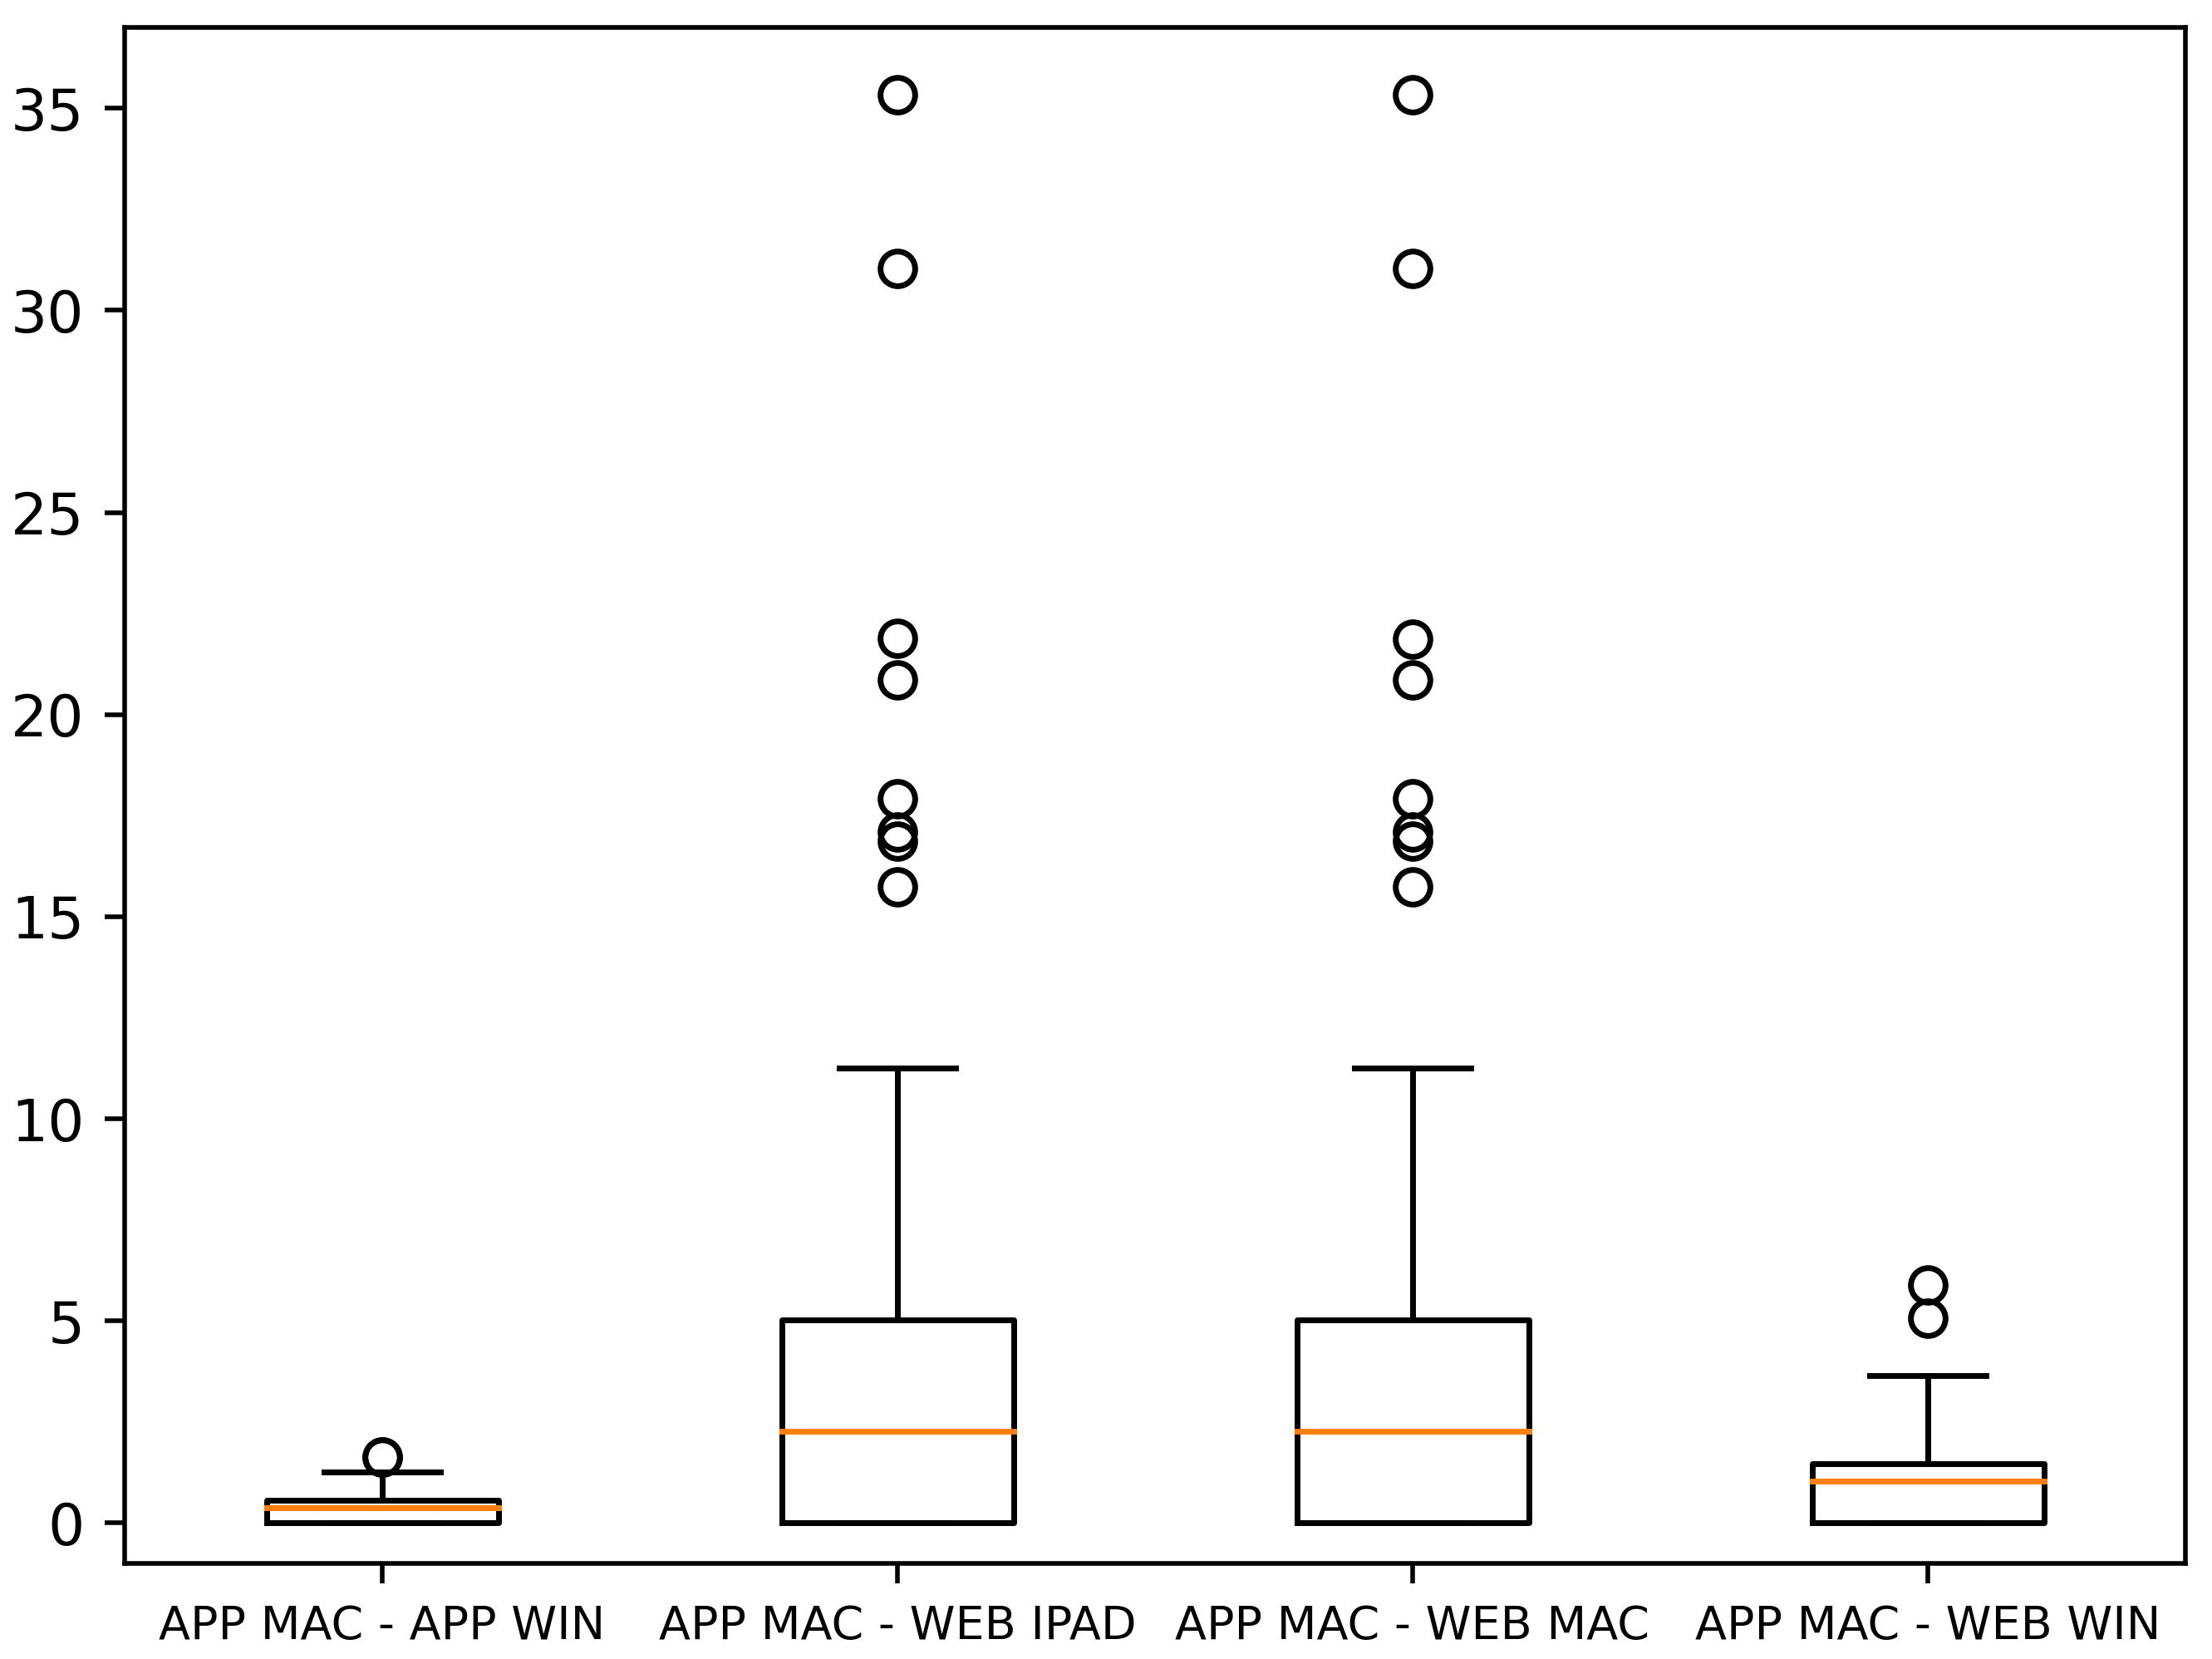
\includegraphics[width=8cm, height=8cm, keepaspectratio]{Immagini/MSE/Immagine1.png}\hspace{1em}
    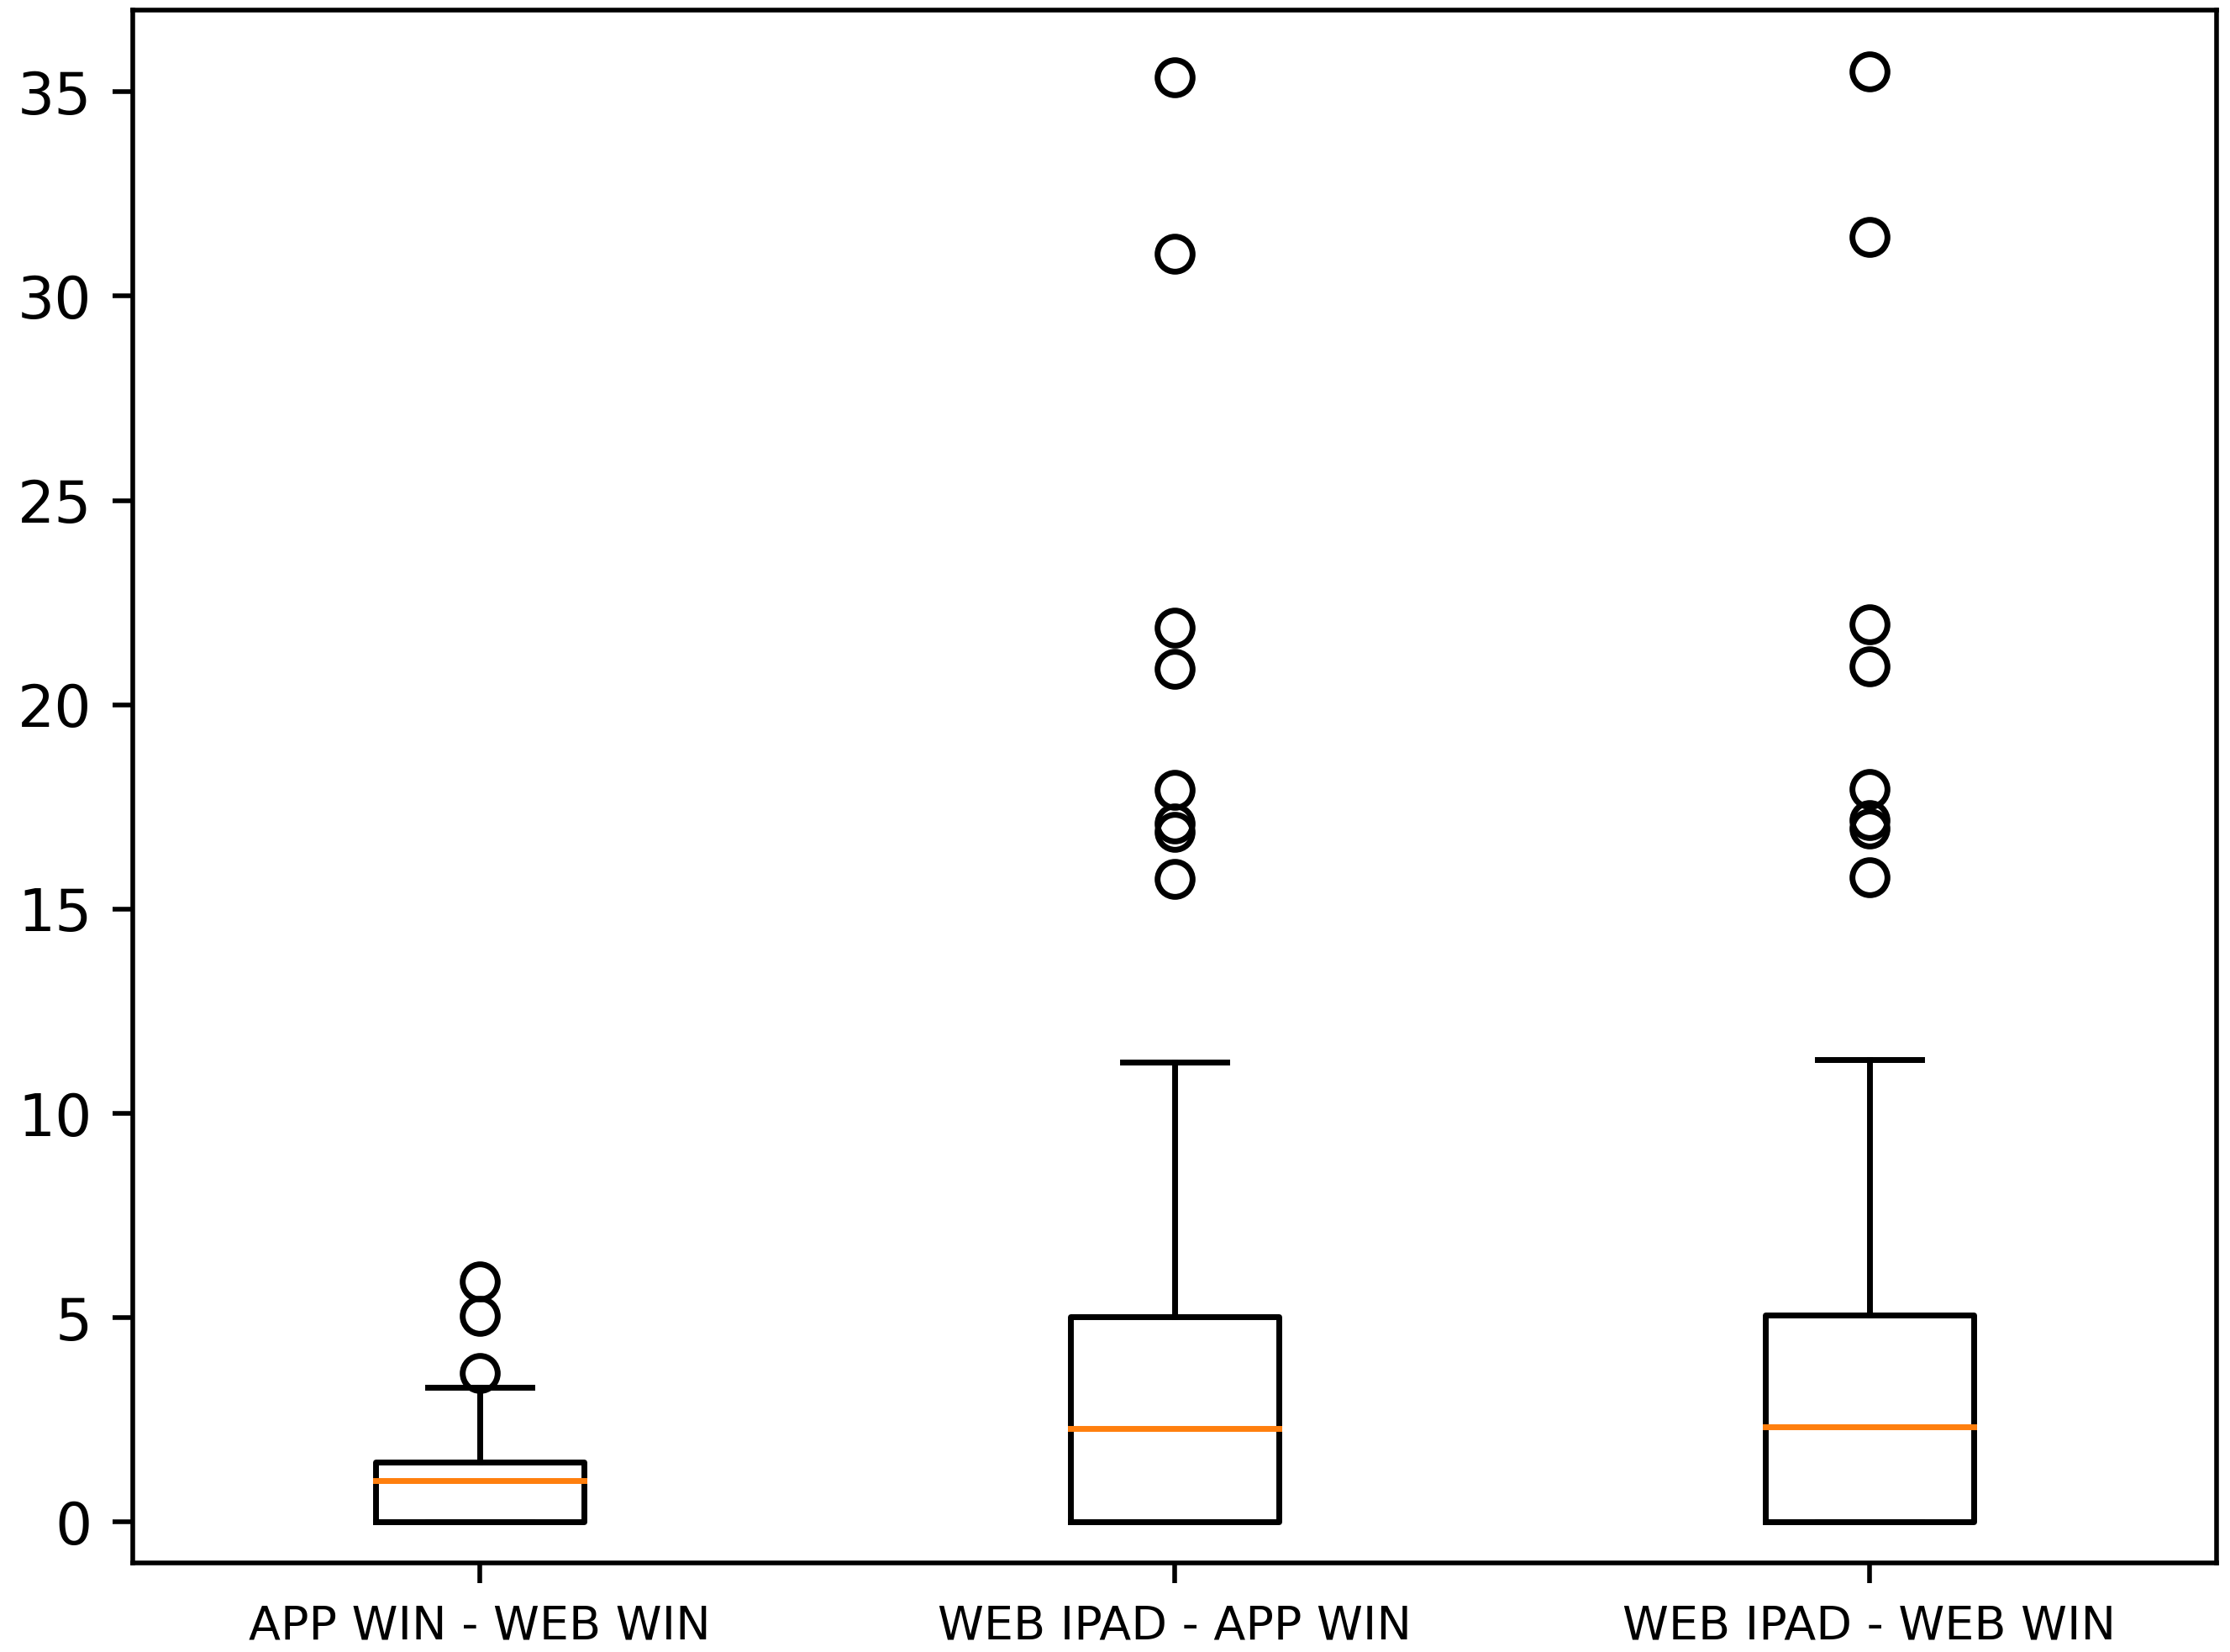
\includegraphics[width=8cm, height=8cm, keepaspectratio]{Immagini/MSE/Immagine2.png}\\\vspace{1em}
    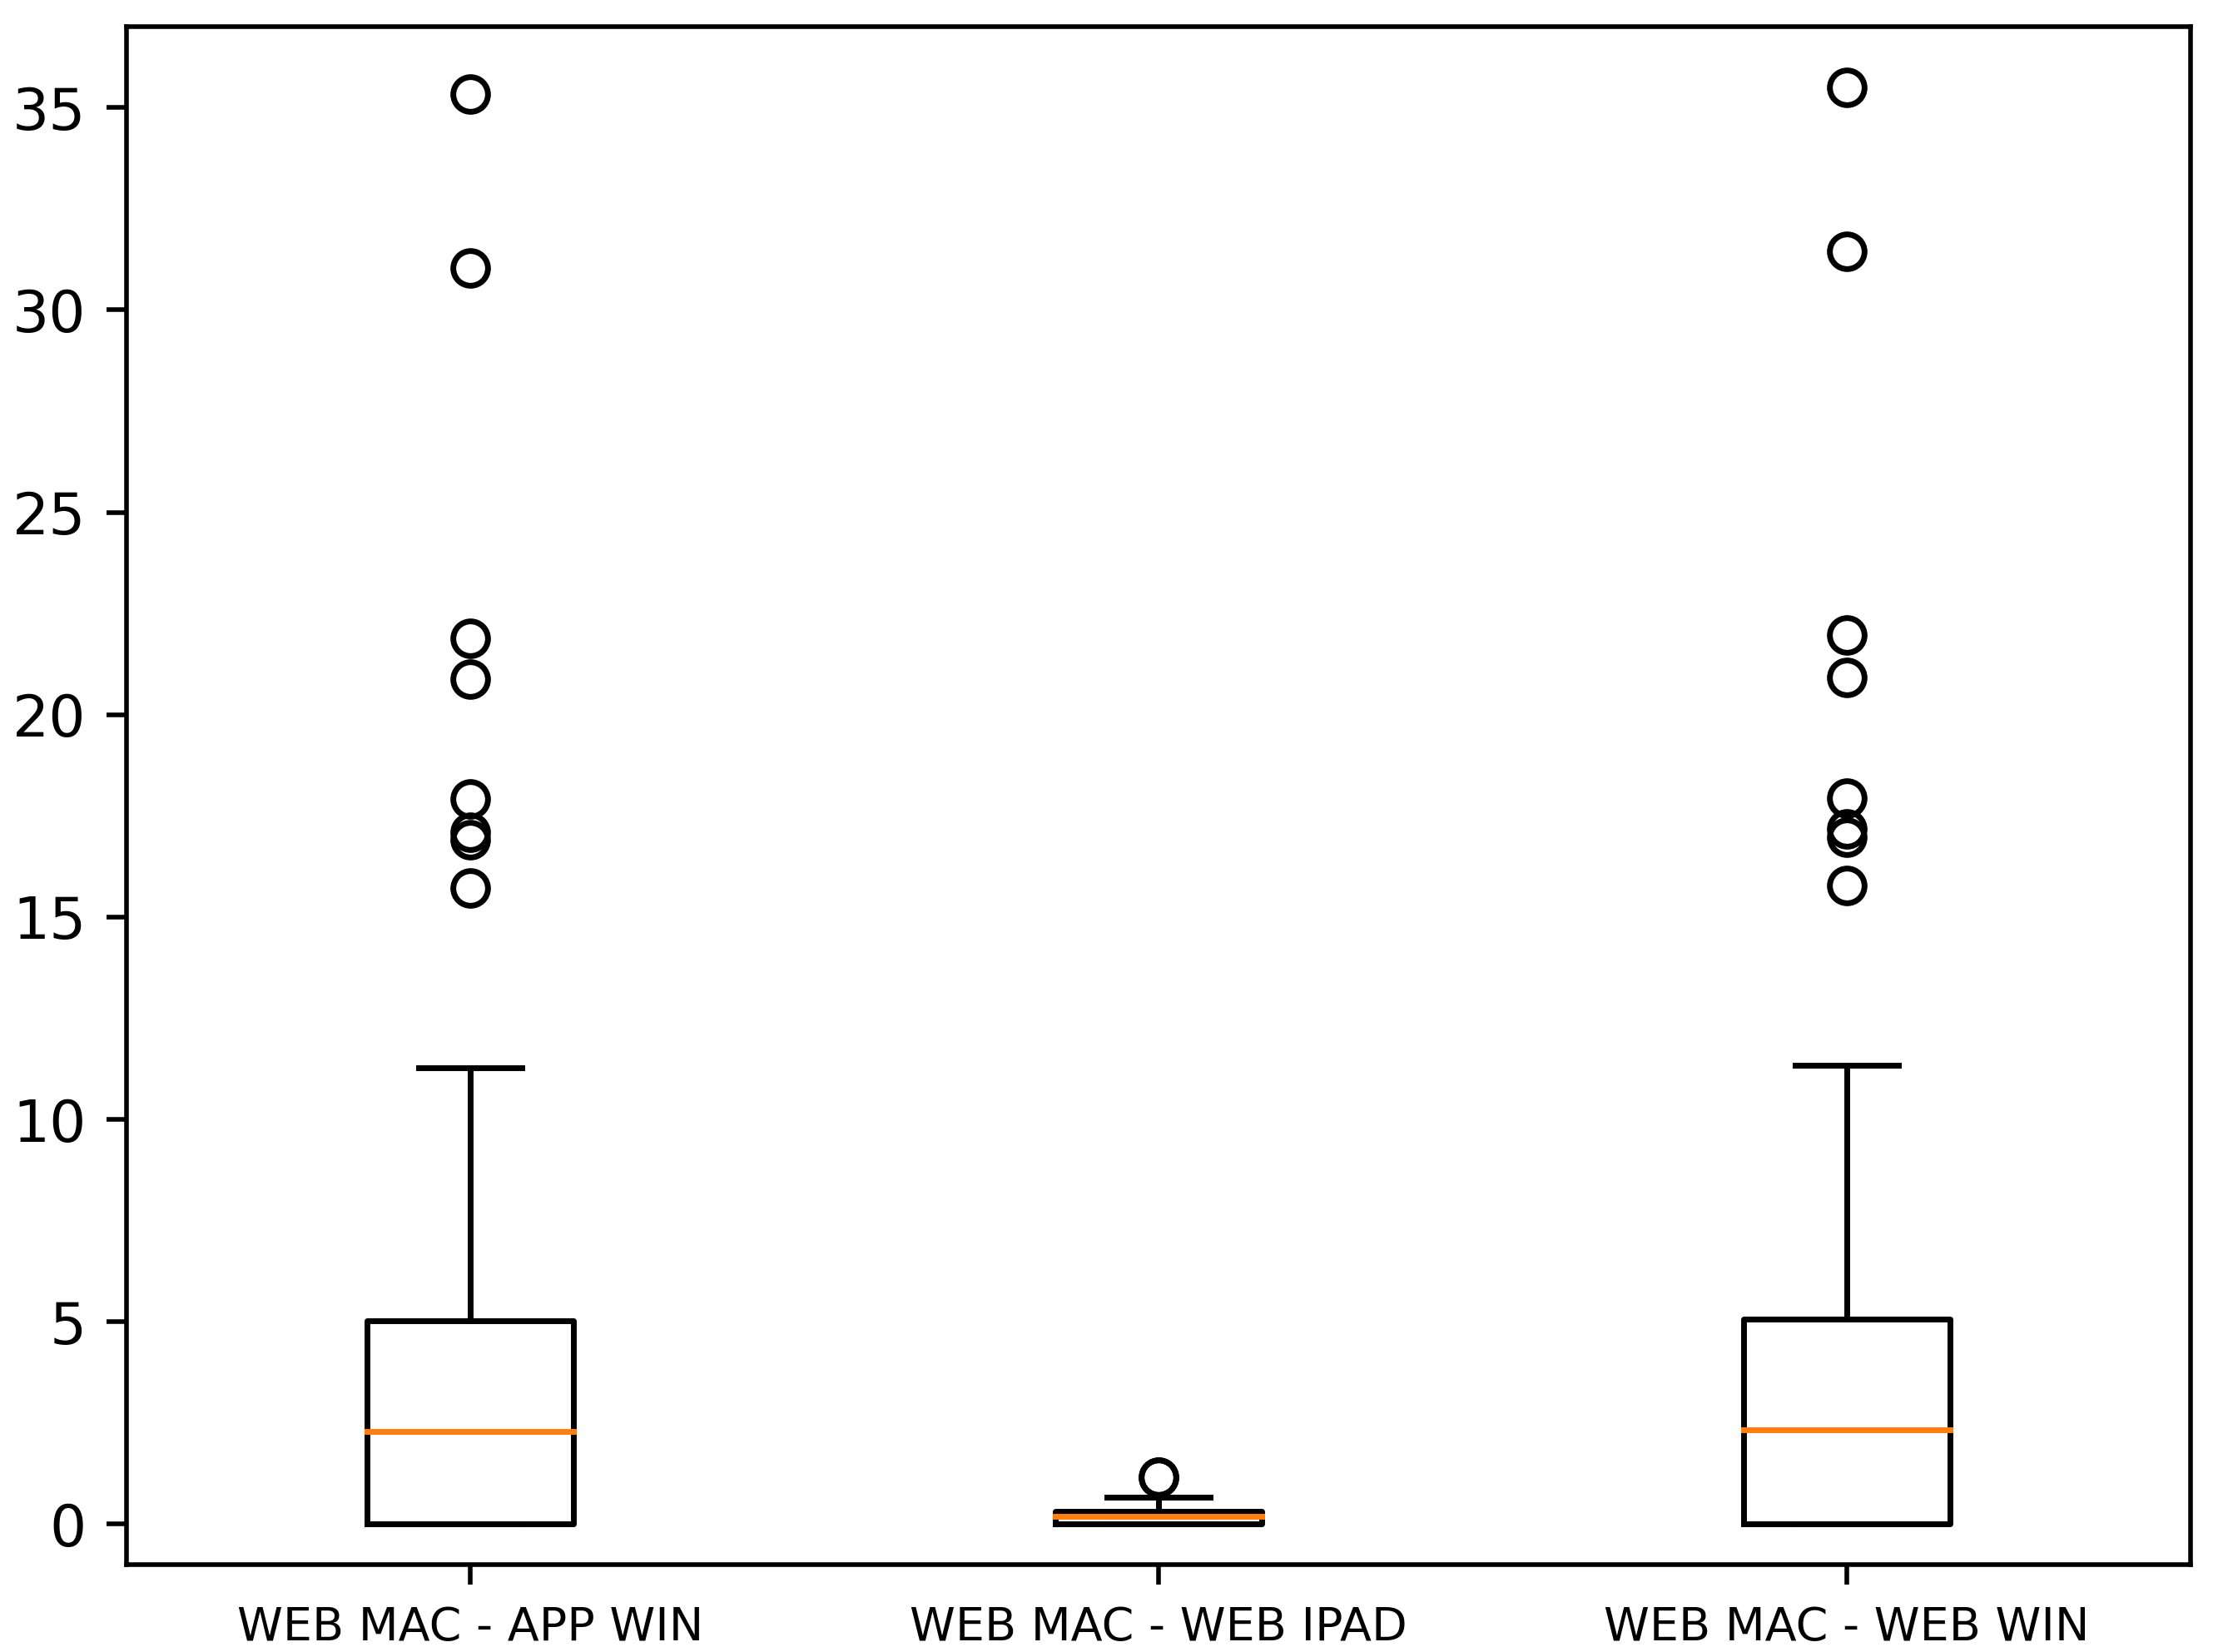
\includegraphics[width=8cm, height=8cm, keepaspectratio]{Immagini/MSE/Immagine3.png}
    \captionof{figure}{Valori del \textit{Mean Square Error} per coppie di metodi di condivisione. I \textit{boxplot} ottenuti sono così formati: la linea arancione corrisponde alla mediana dei valori; il rettangolo costituisce l'intervallo interquartile; la linea sopra indica il terzo quartile mentre i cerchi corrispondono agli \textit{outliers}.}
    \label{fig:mse_results}
\endgroup

% \begin{figure}[h!]
%     \centering
%     \subfloat[][]{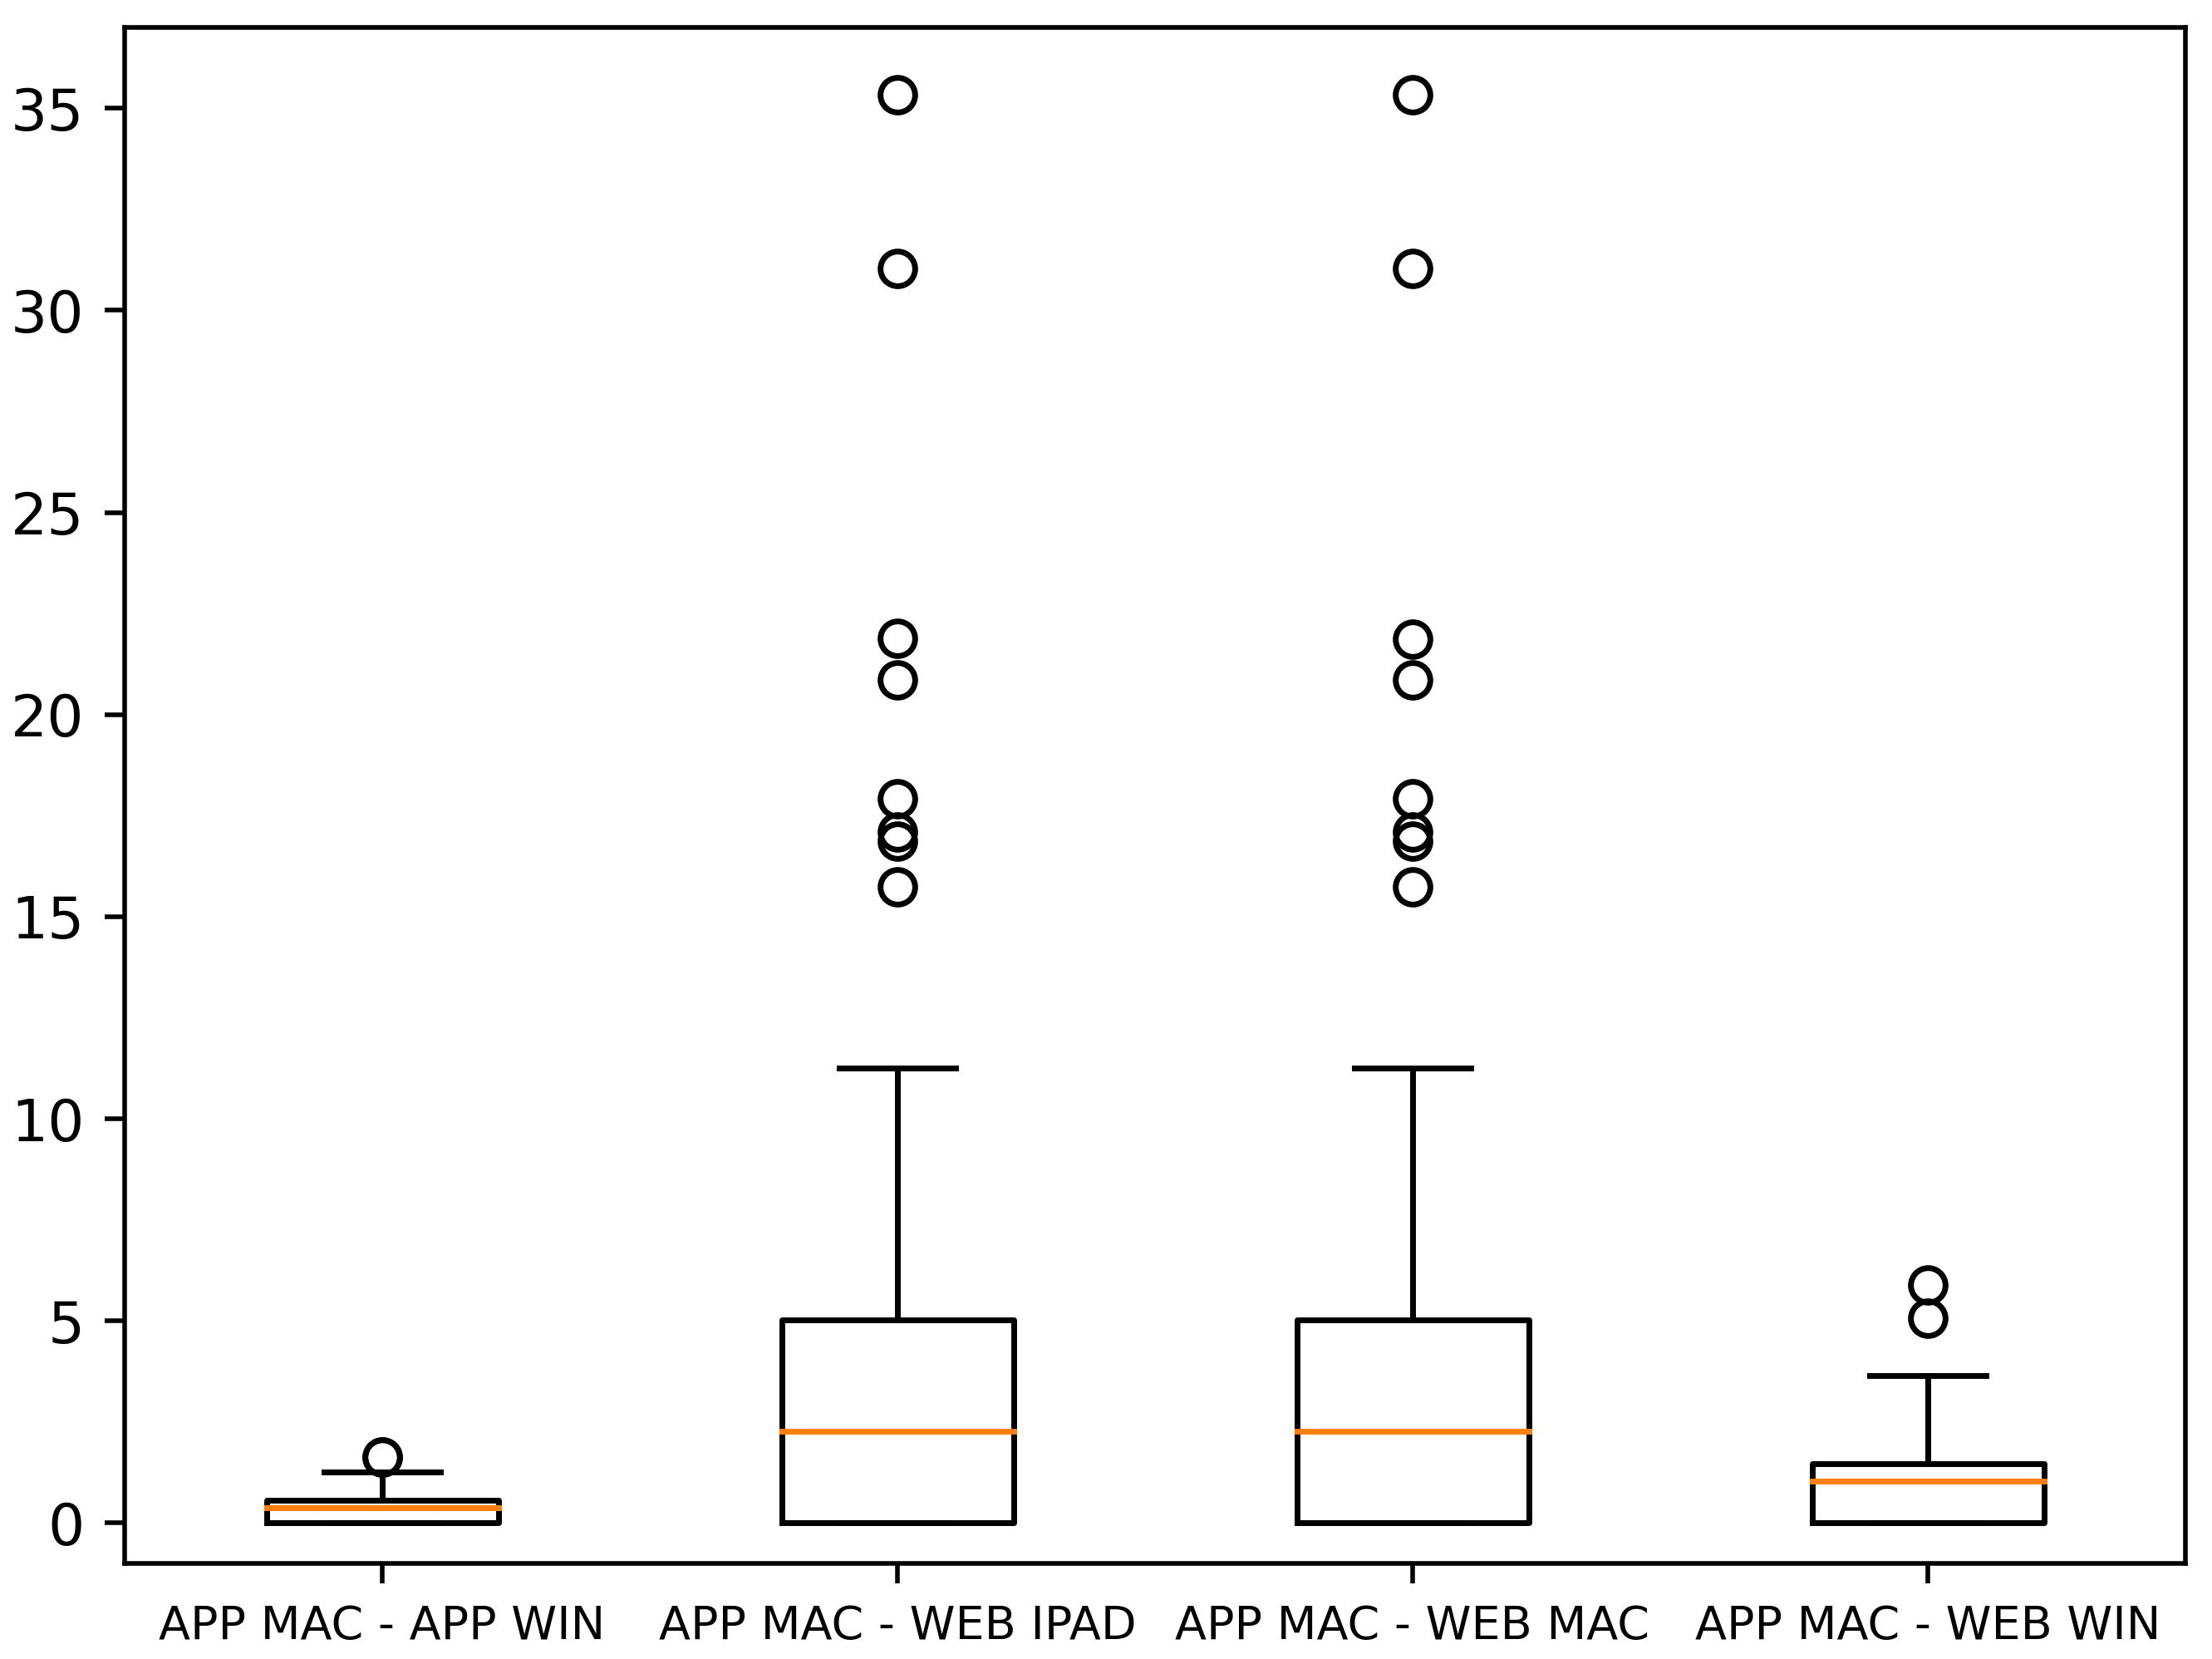
\includegraphics[width=8cm, height=8cm, keepaspectratio]{Immagini/MSE/Immagine1.png}}\hspace{1em}
%     \subfloat[][]{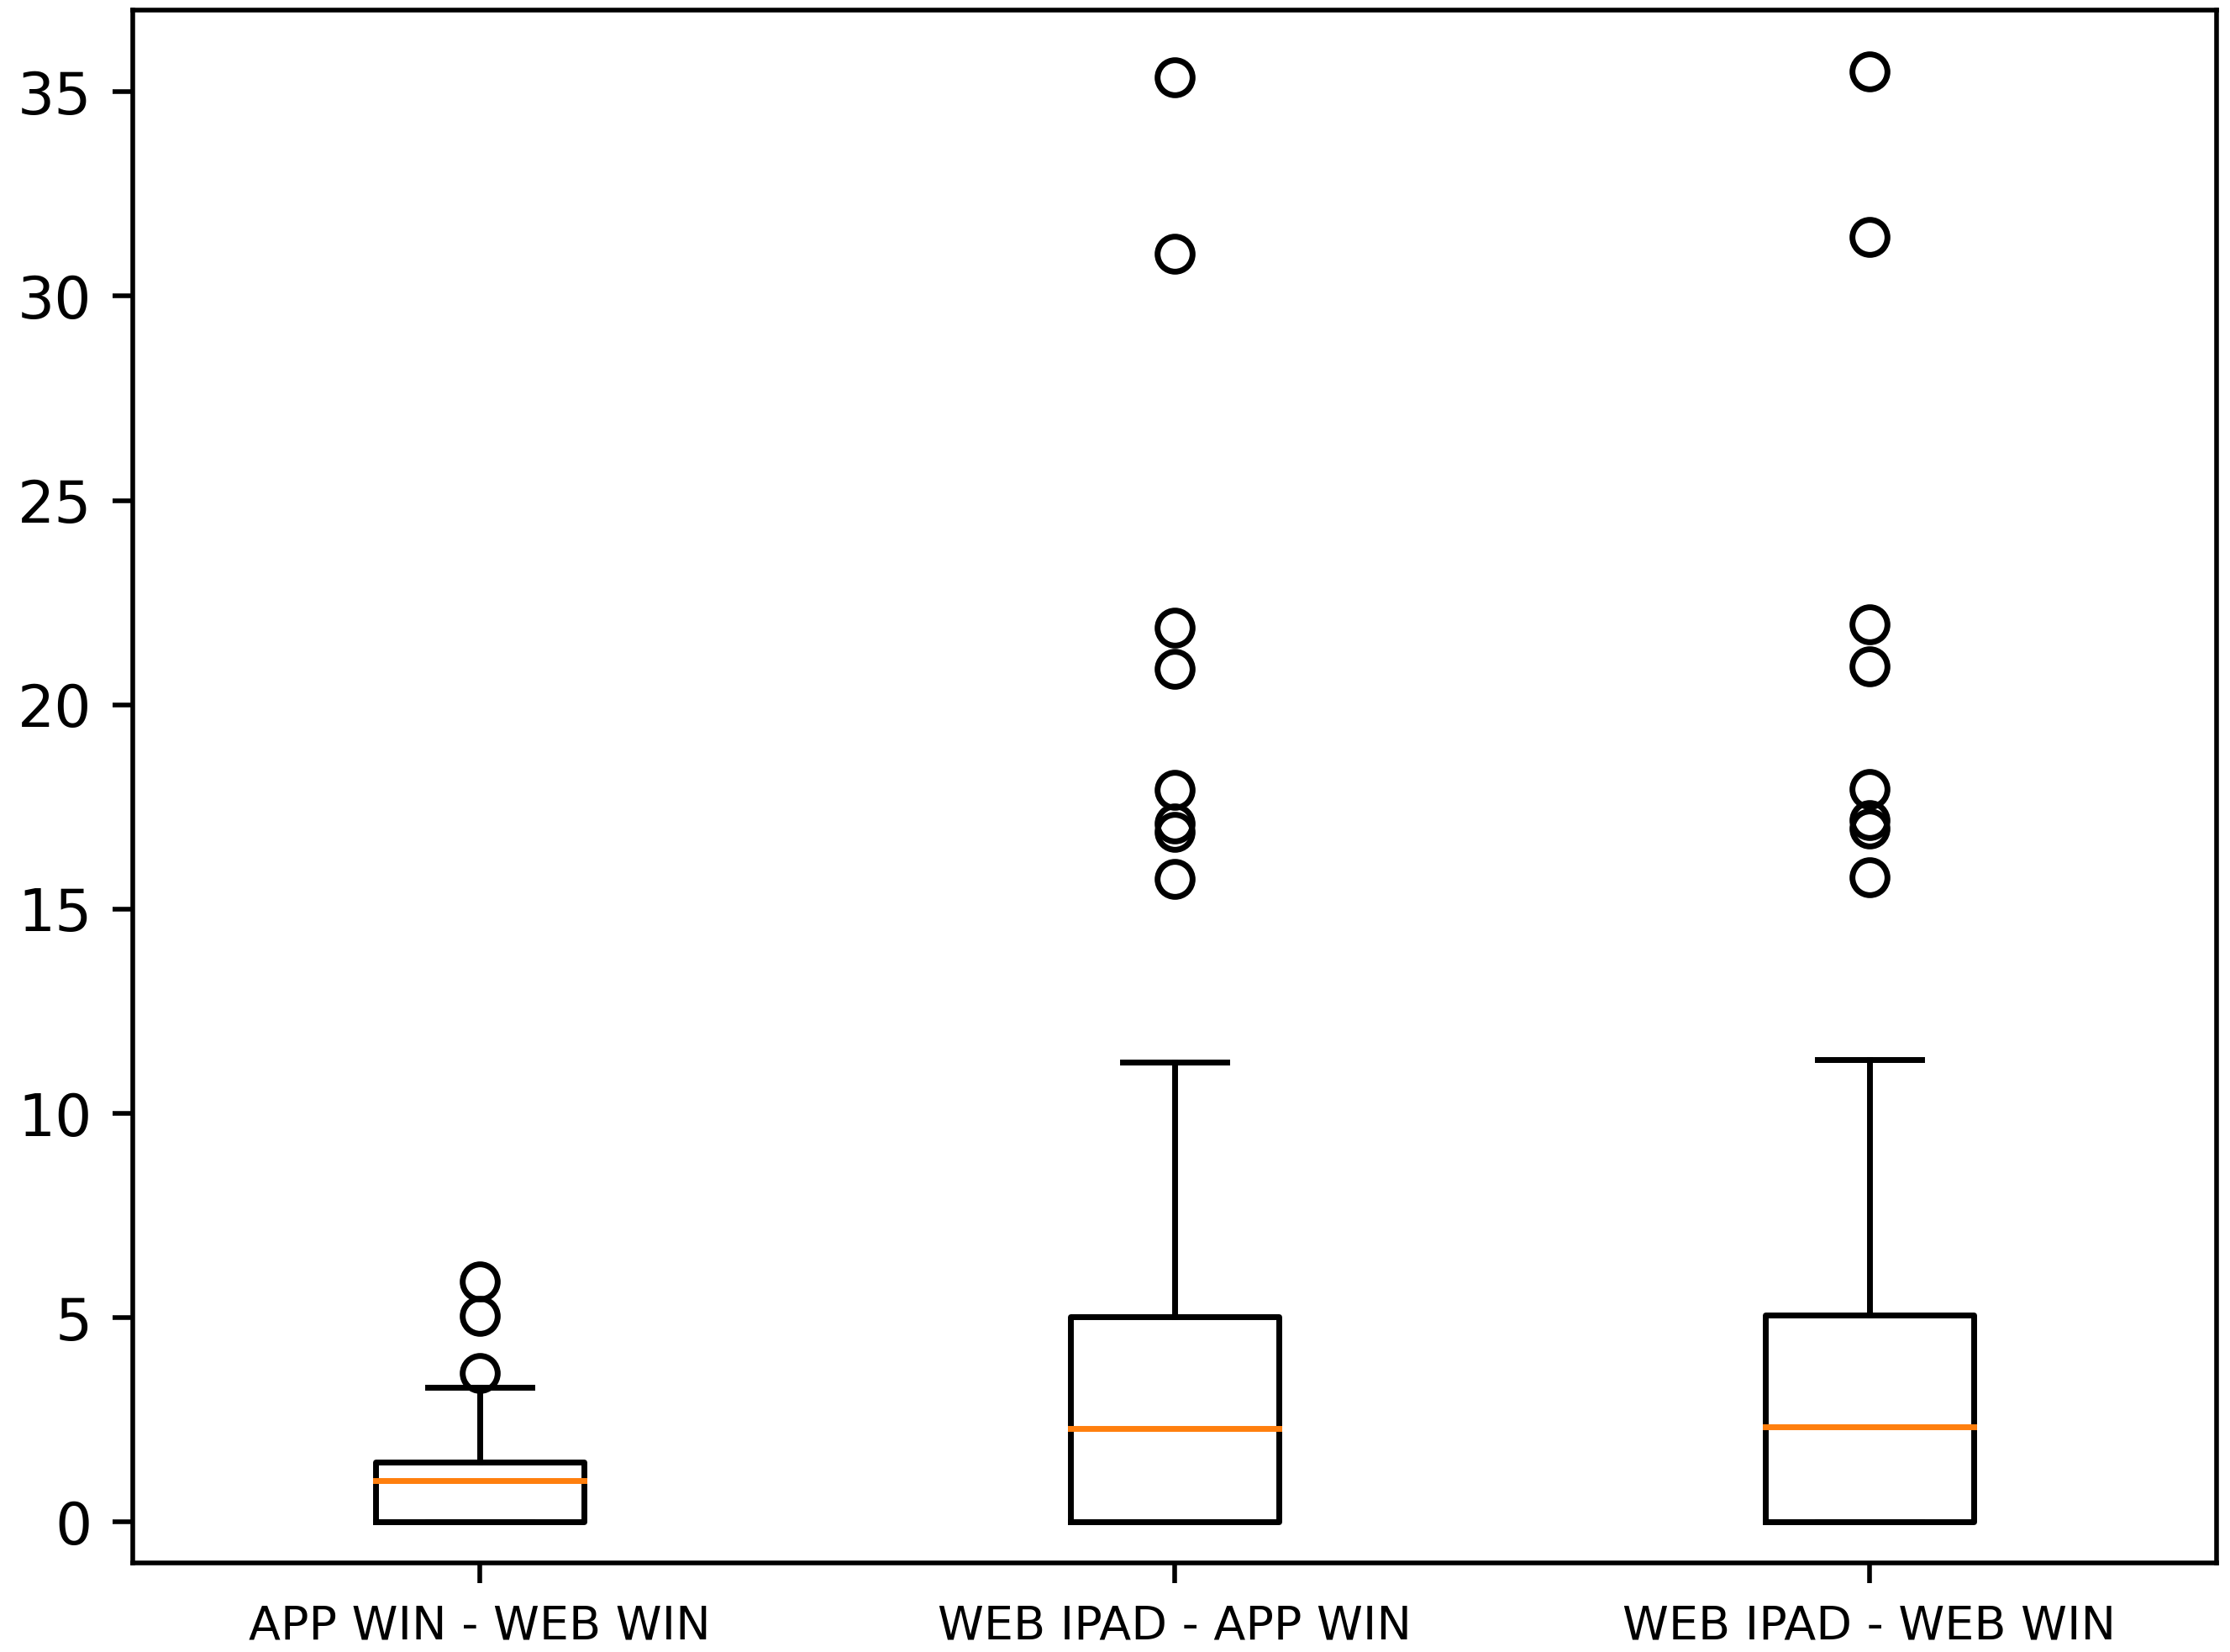
\includegraphics[width=8cm, height=8cm, keepaspectratio]{Immagini/MSE/Immagine2.png}}\\\vspace{1em}
%     \subfloat[][]{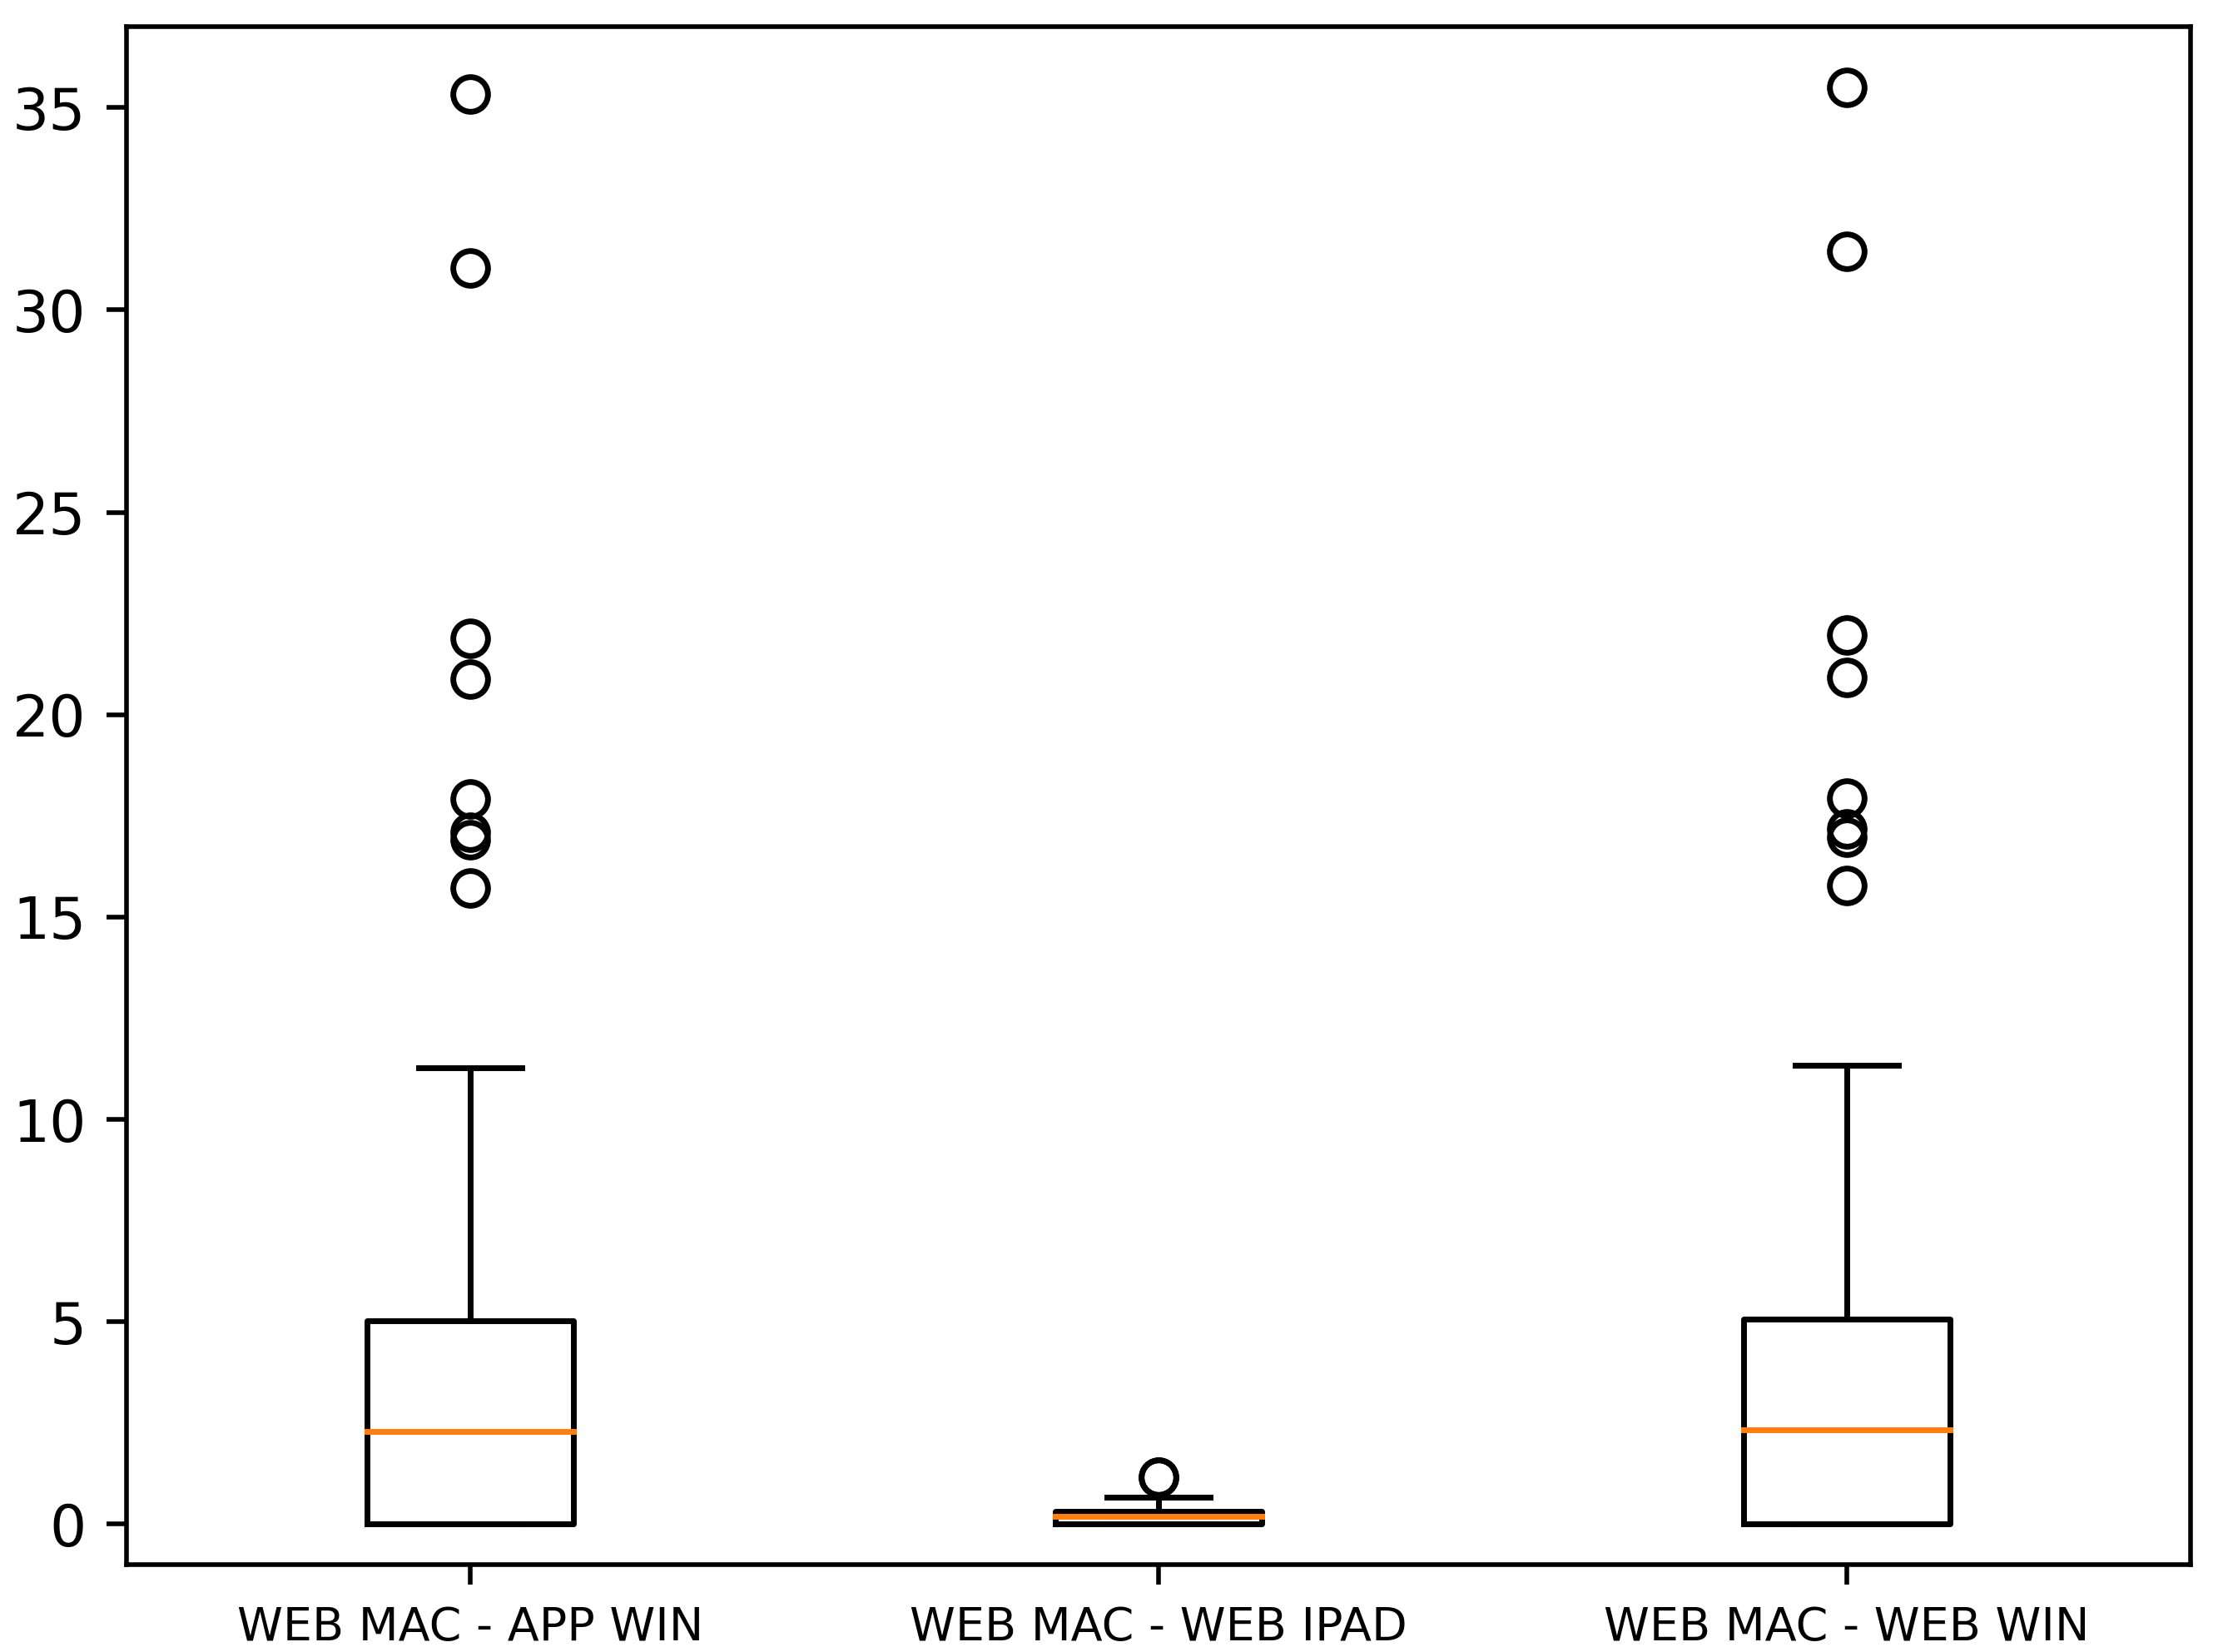
\includegraphics[width=8cm, height=8cm, keepaspectratio]{Immagini/MSE/Immagine3.png}}
%     \caption{Valori del \textit{Mean Square Error} per coppie di metodi di condivisione. I \textit{boxplot} ottenuti sono così formati: la linea arancione corrisponde alla mediana dei valori; il rettangolo costituisce l'intervallo interquartile; le linee sopra indicano il primo quartile mentre i cerchi corrispondono agli \textit{outliers}.}
%     \label{fig:mse_results}
% \end{figure}

\vspace{2em}

Guardando ai grafici ottenuti per il \textit{Peak Signal-to-Noise Ratio} in Fig.~\ref{fig:psnr_results} e in particolare all'elevato range di valori, si evidenzia come il livello di compressione applicato sulle immagini da WhatsApp non abbia particolarmente impattato sulla loro qualità. Notare come le coppie di immagini per cui il calcolo del MSE ha dato risultato 0 non siano presenti per le ragioni citate nel capitolo precedente. I pattern riscontrati per i risultati del MSE sono identificabili anche nel caso del PSNR.\\

% \begin{figure}[h!]
%     \centering
%     \subfloat[][]{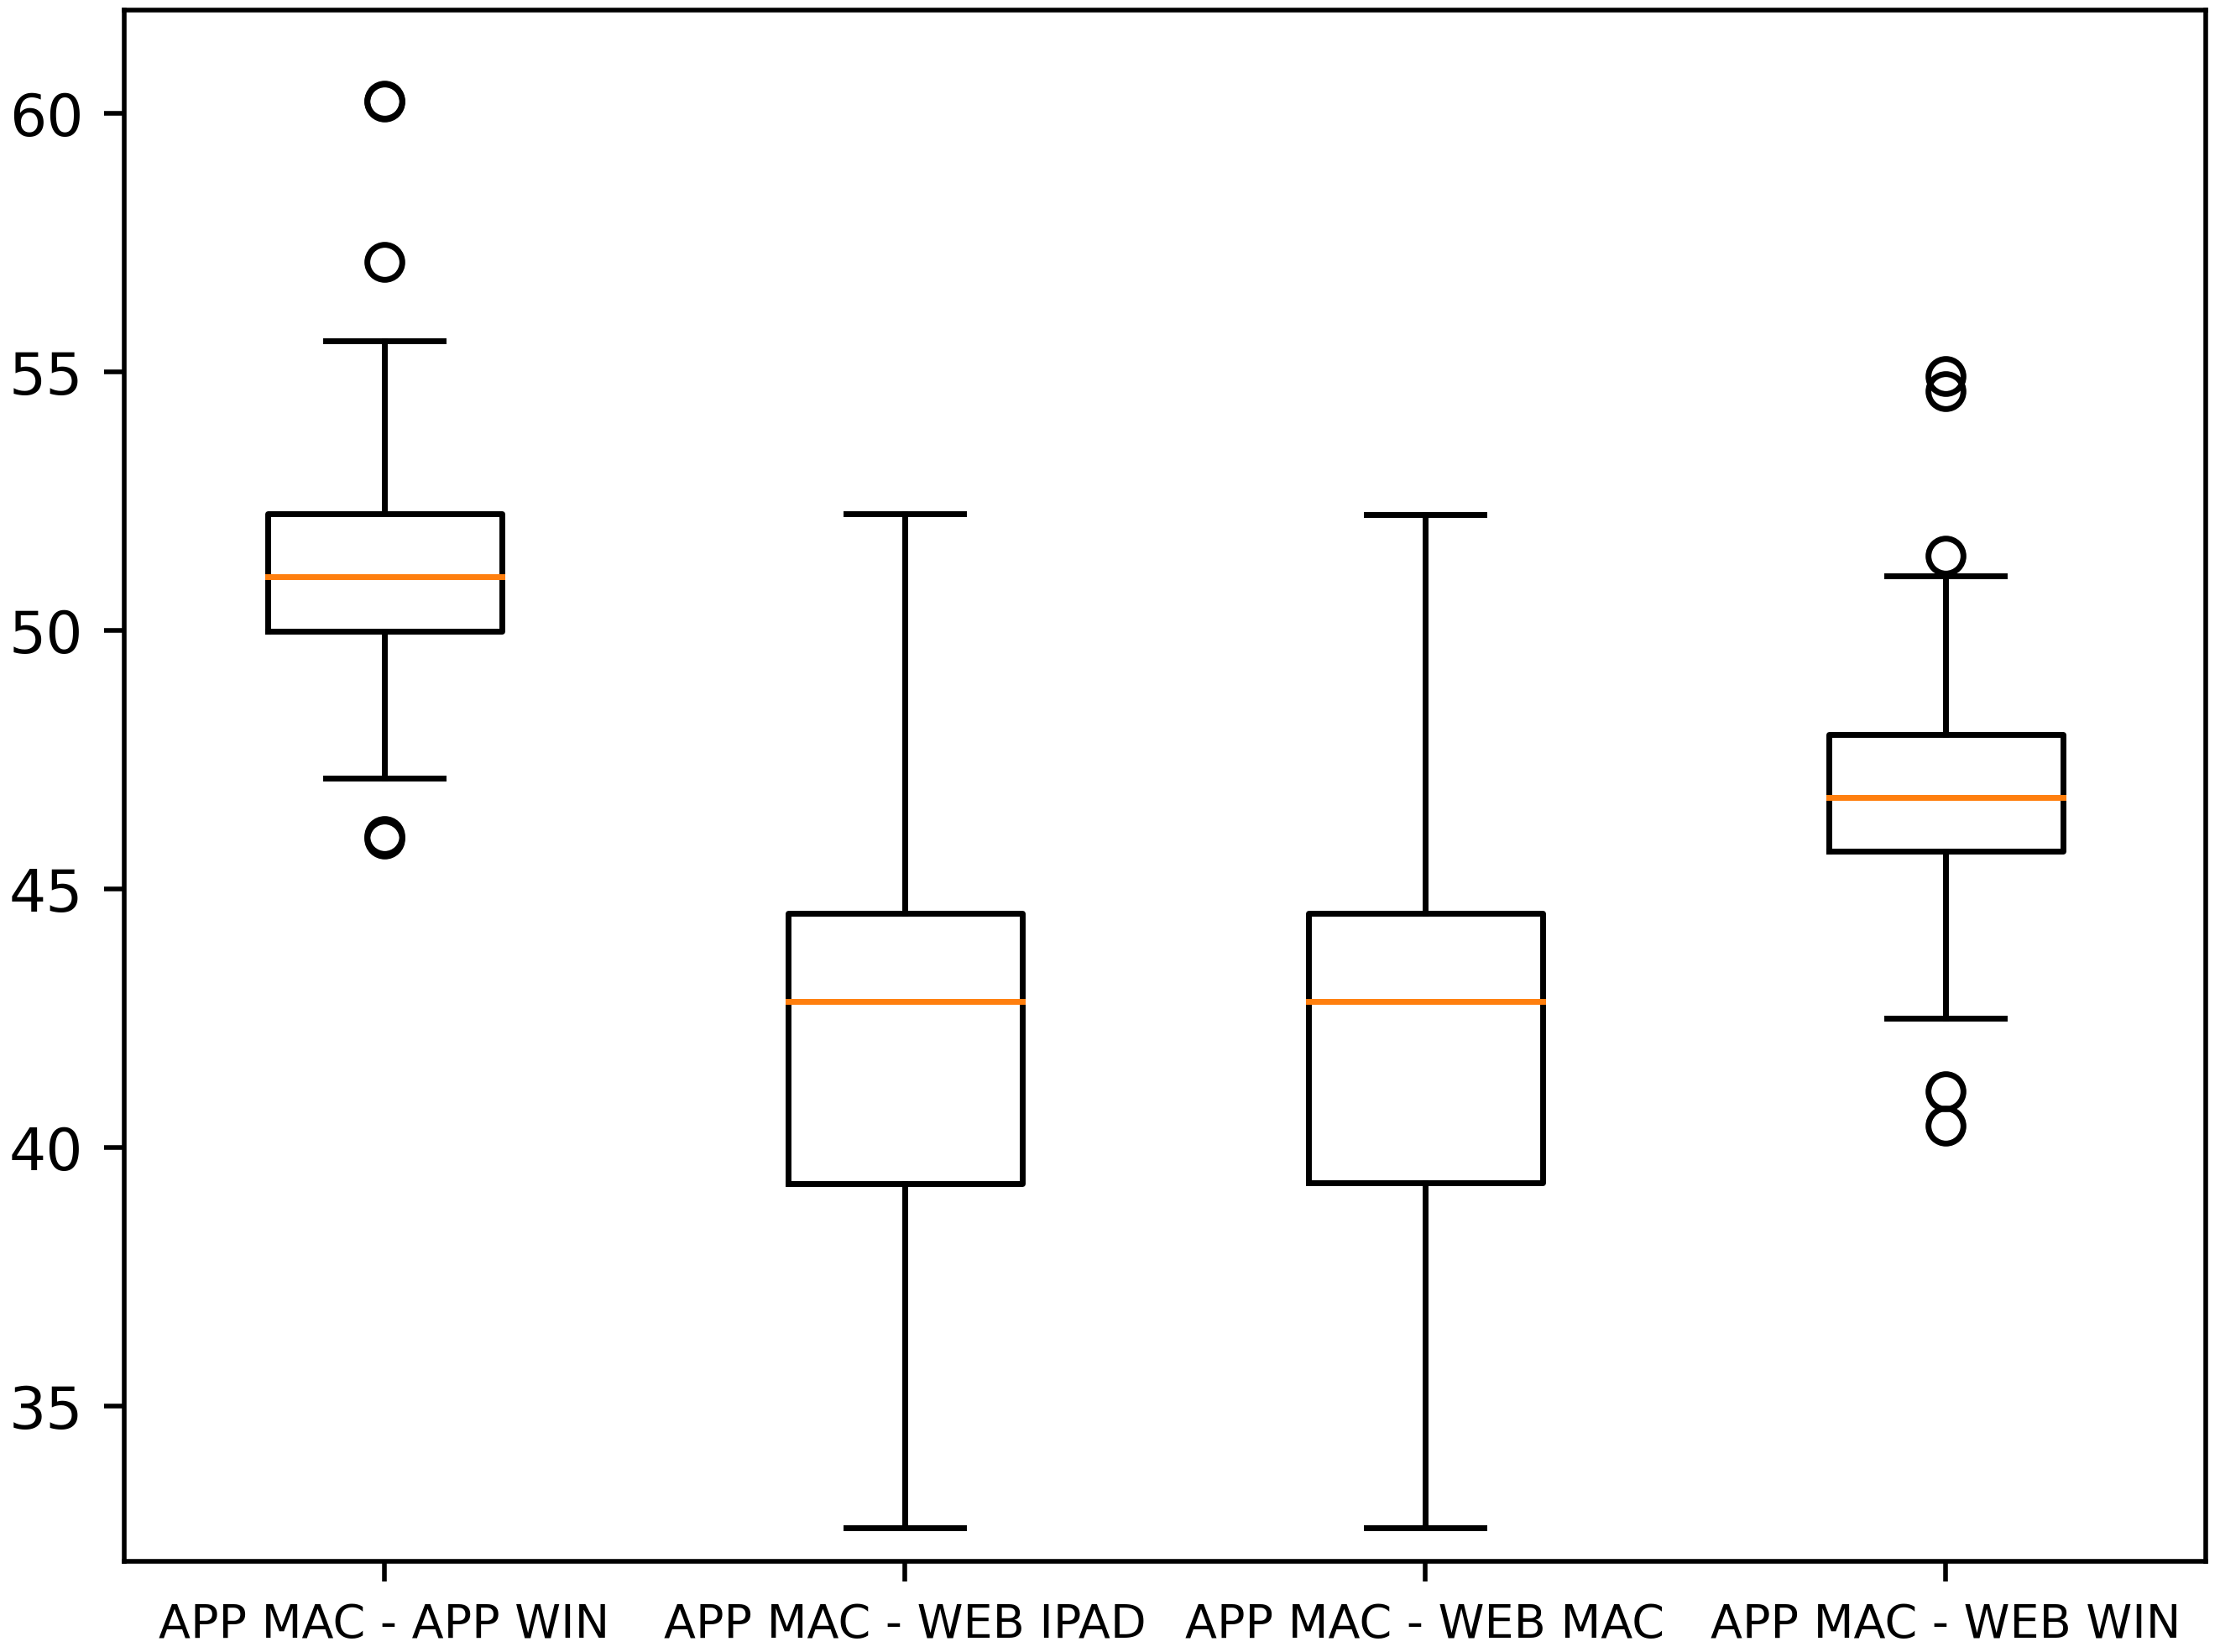
\includegraphics[width=8cm, height=8cm, keepaspectratio]{Immagini/PSNR/Immagine1.png}}\hspace{1em}
%     \subfloat[][]{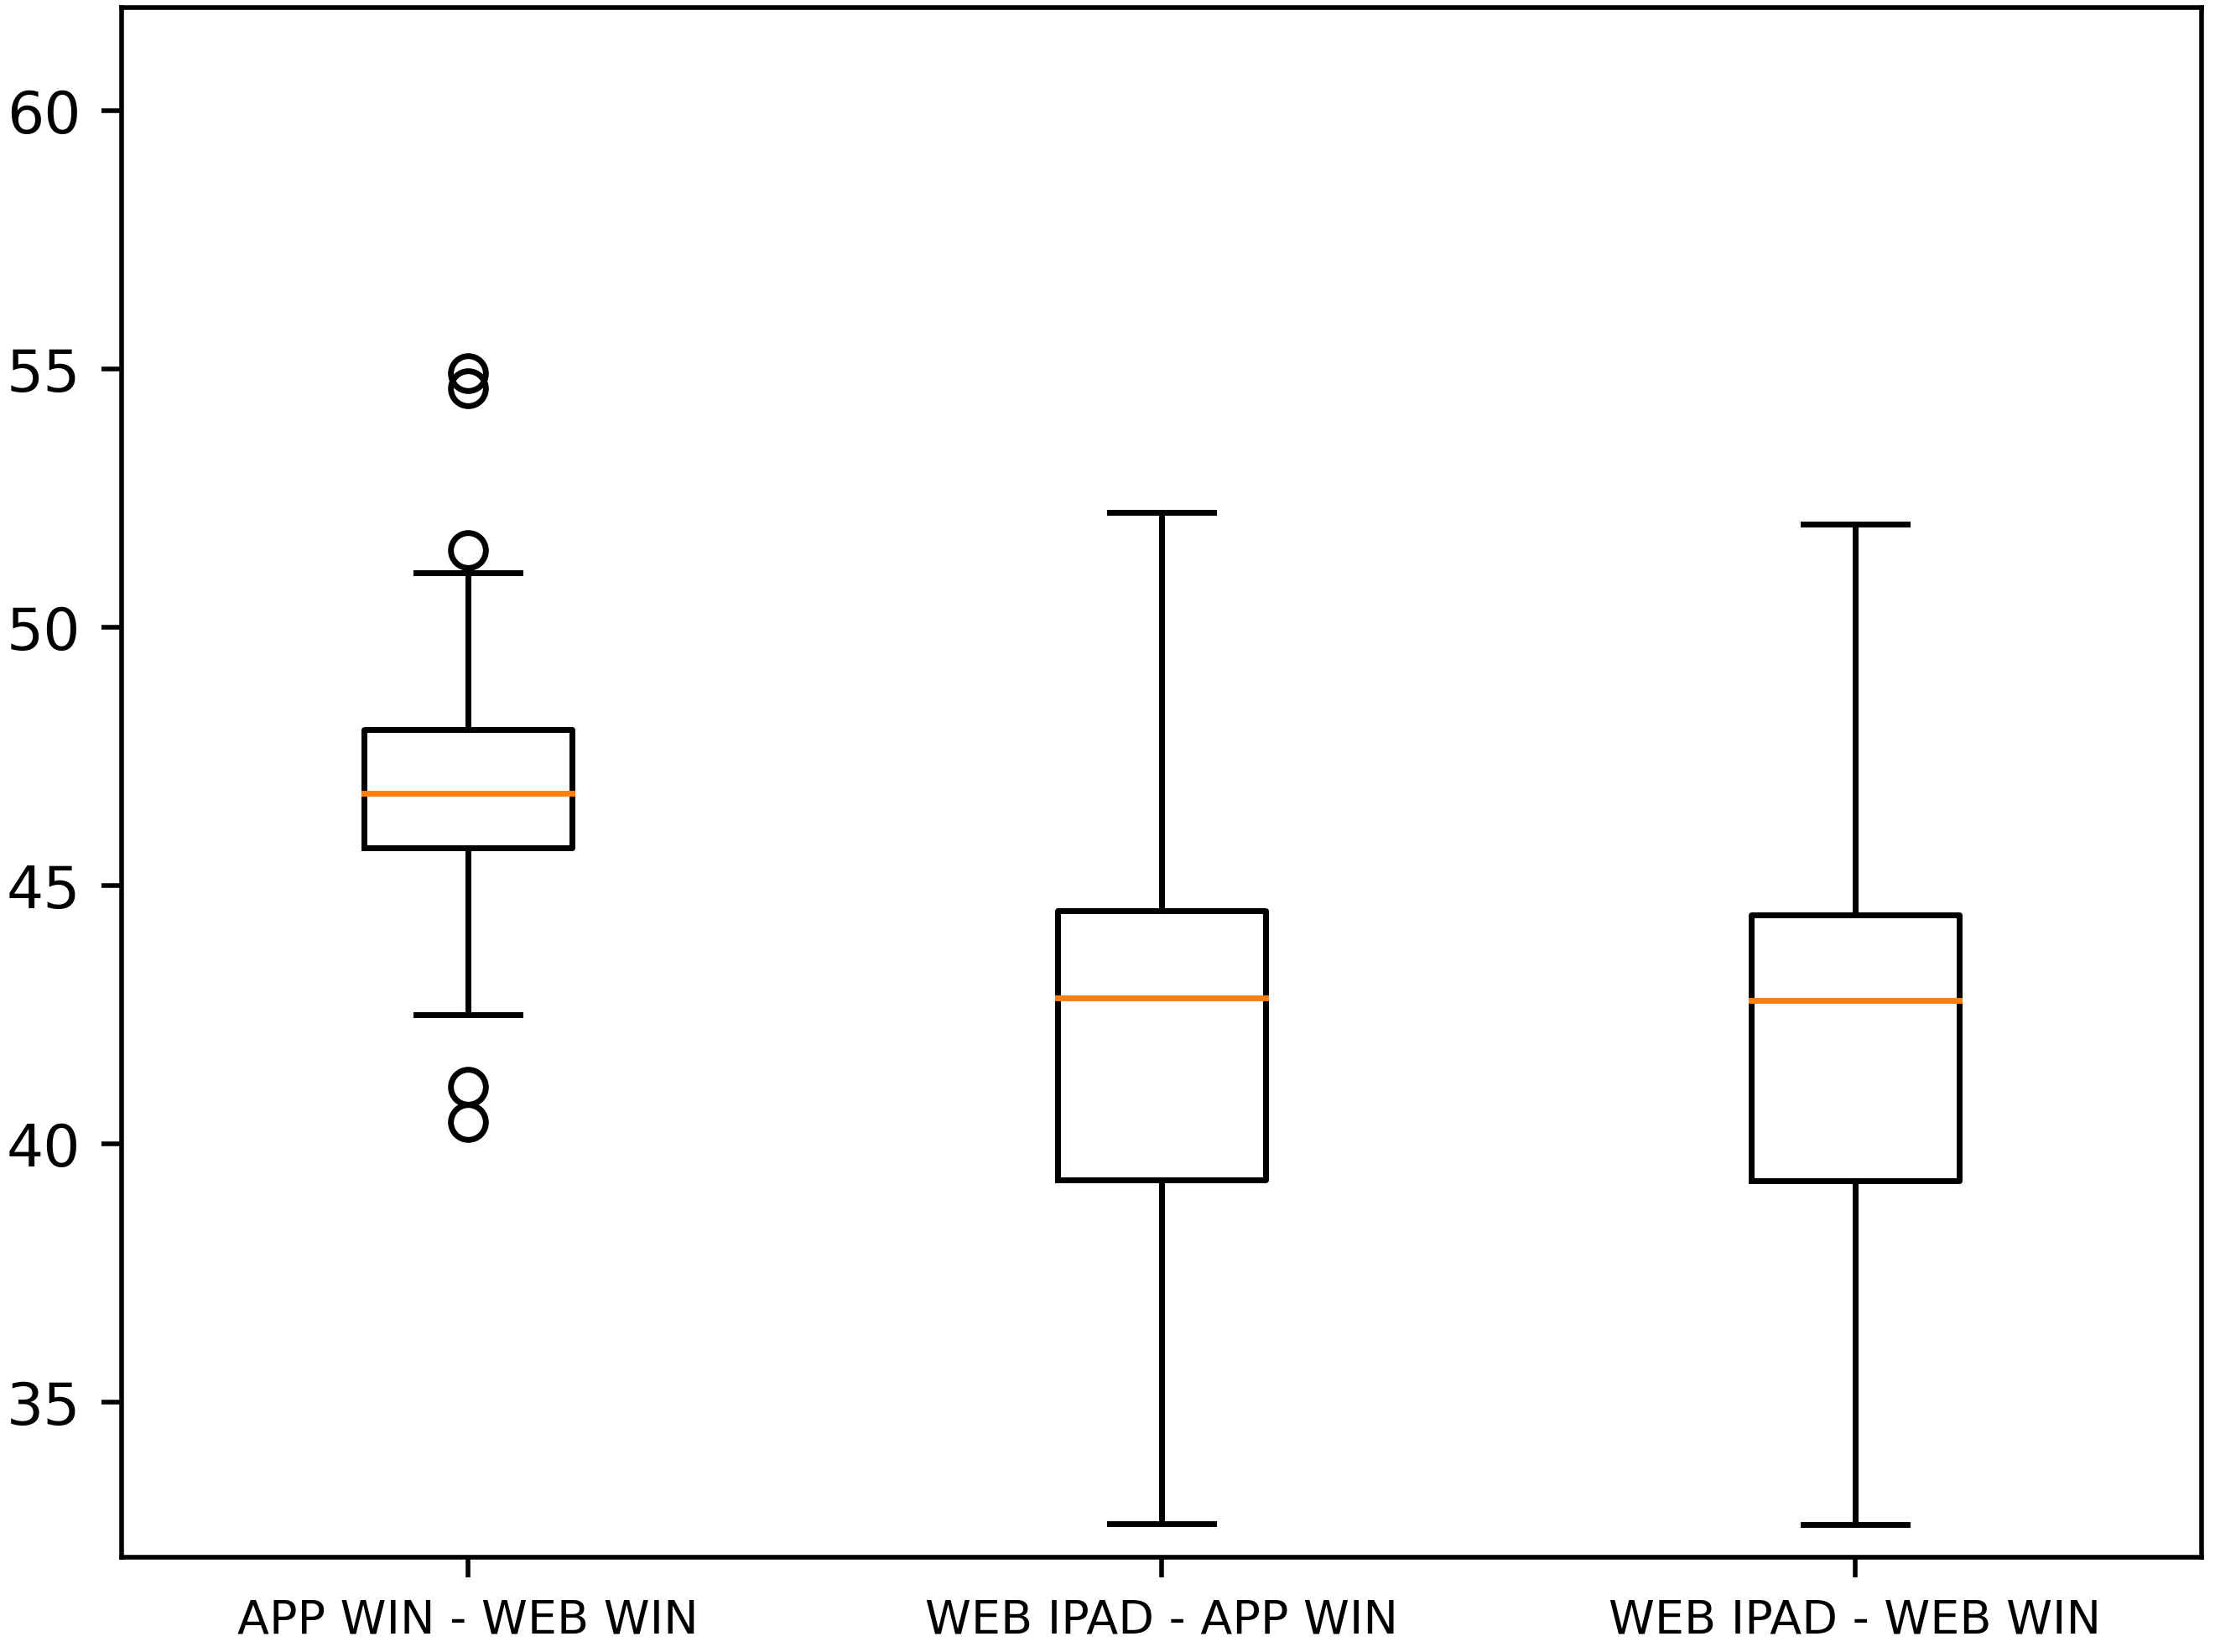
\includegraphics[width=8cm, height=8cm, keepaspectratio]{Immagini/PSNR/Immagine2.png}}\\\vspace{1em}
%     \subfloat[][]{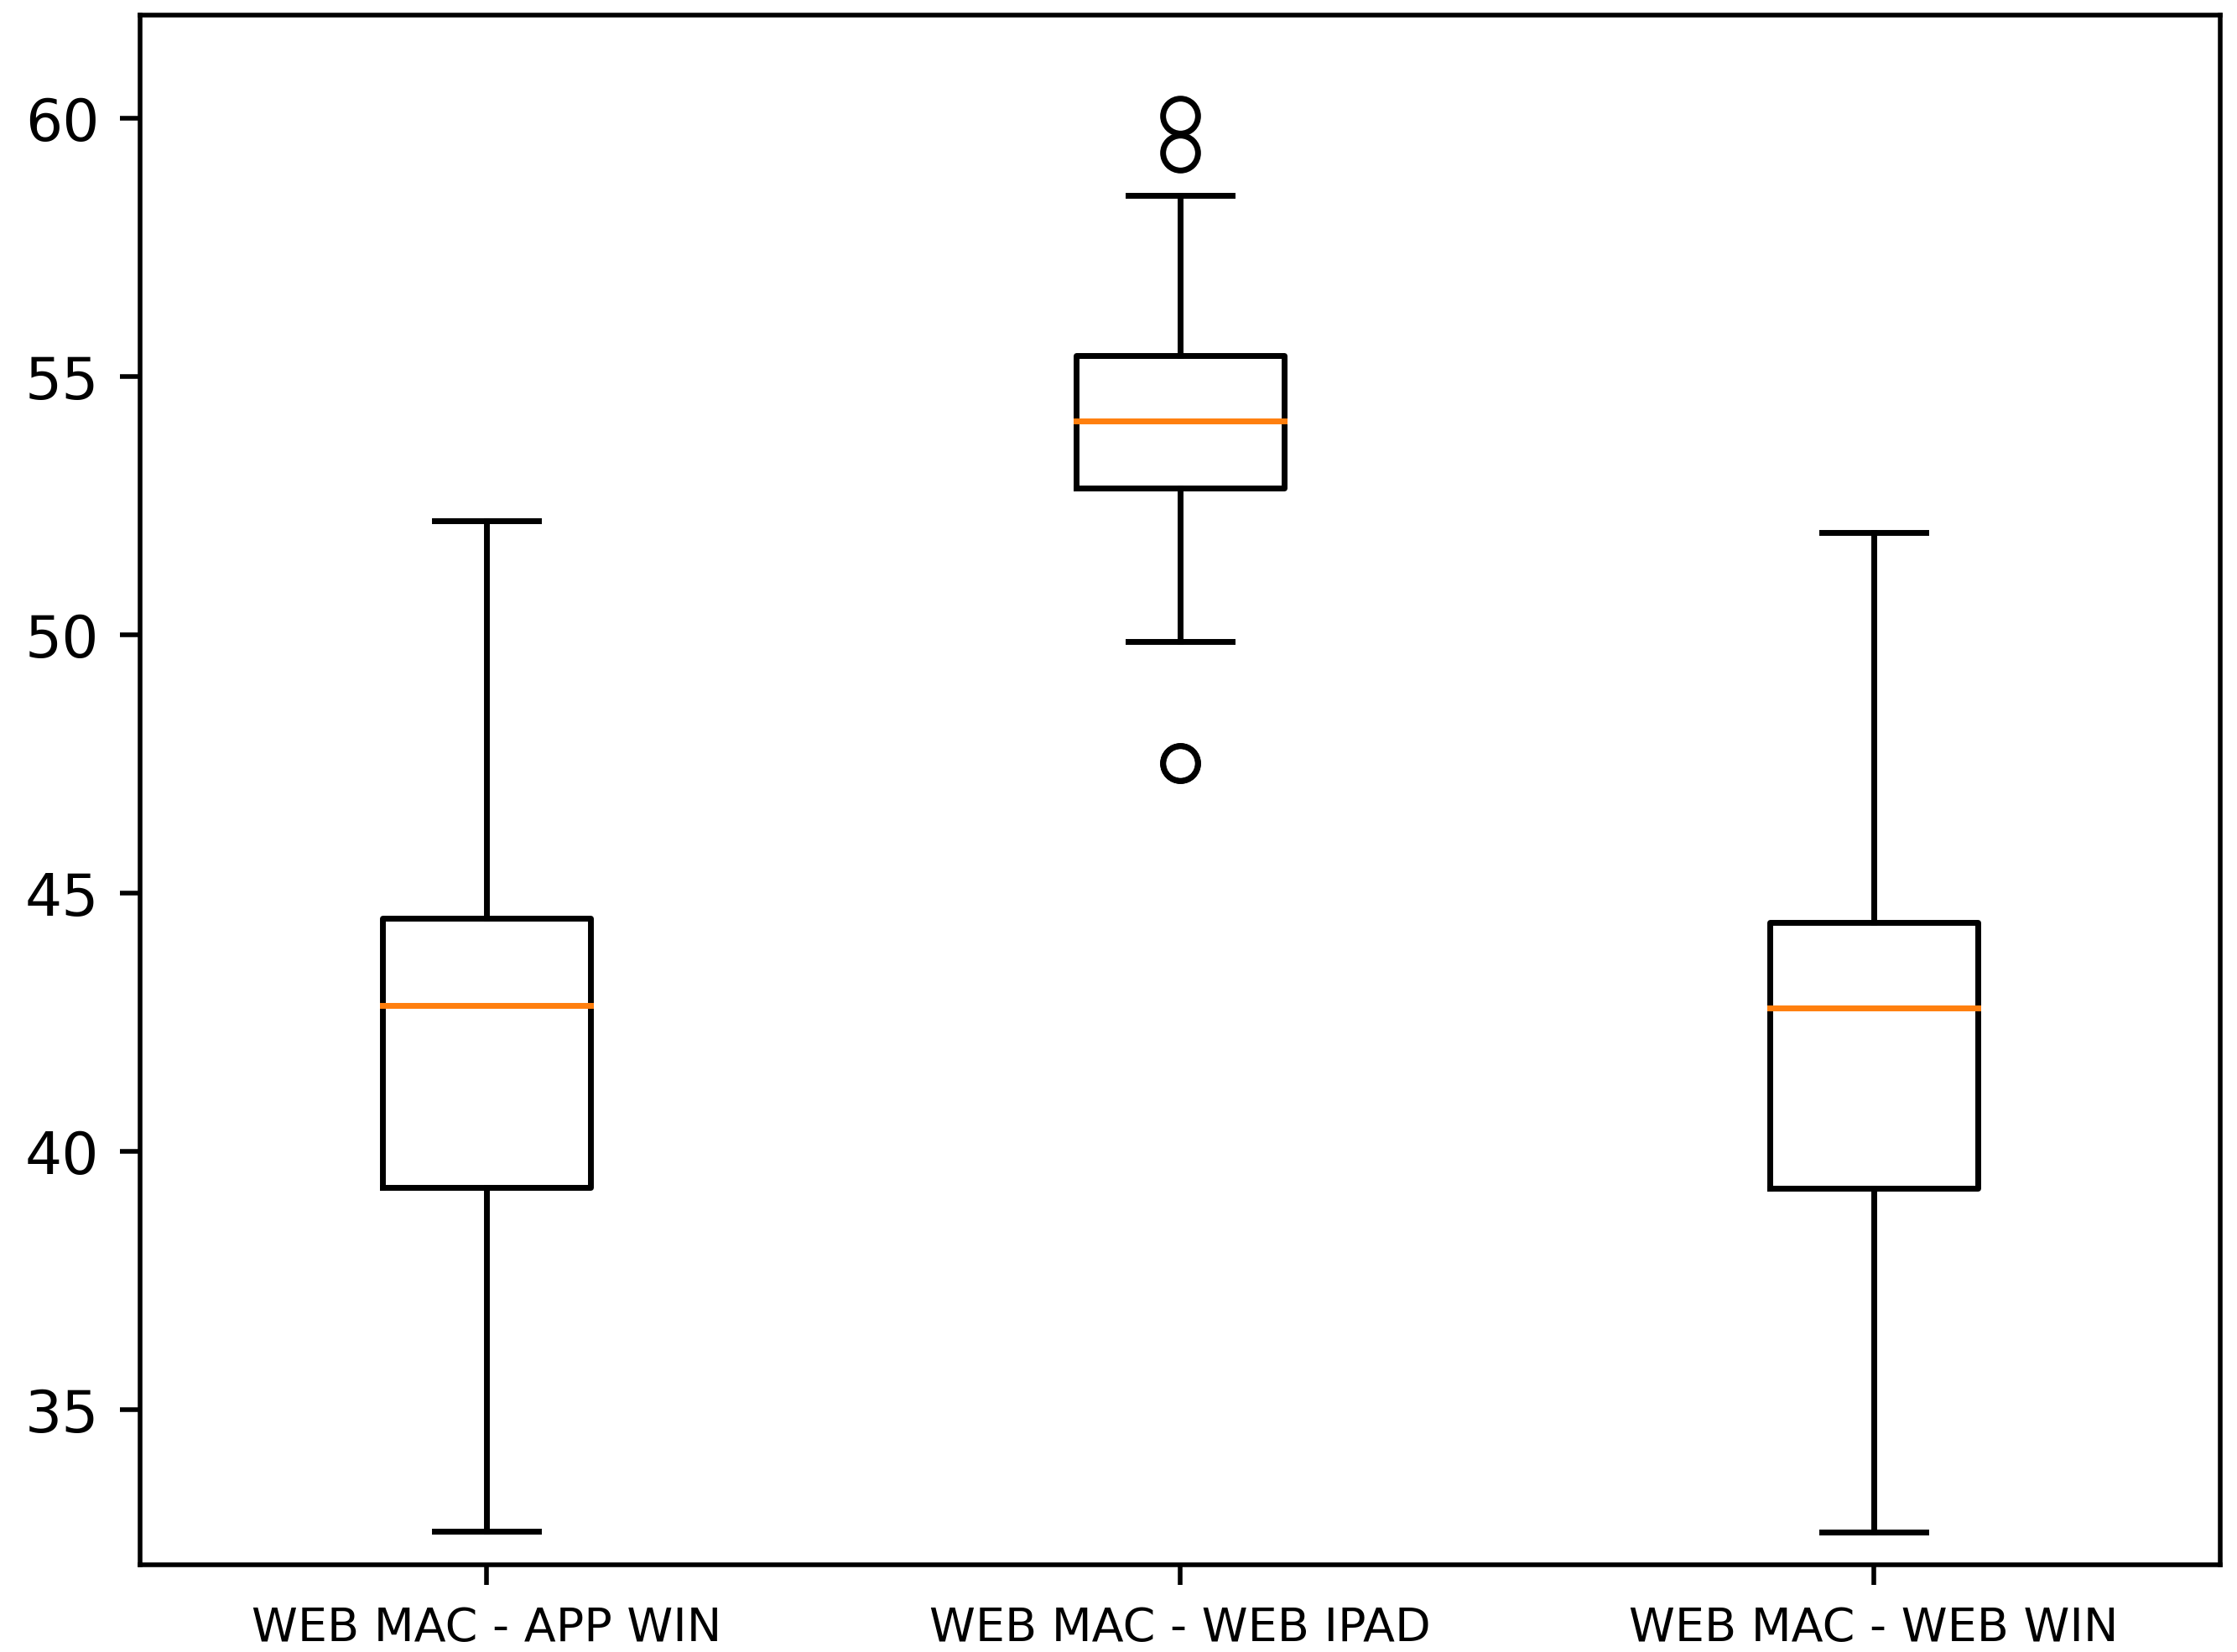
\includegraphics[width=8cm, height=8cm, keepaspectratio]{Immagini/PSNR/Immagine3.png}}\\
%     \caption{\textit{Boxplot} ricavati dal calcolo del PSNR}
%     \label{fig:psnr_results}
% \end{figure}

\begingroup
    \centering
    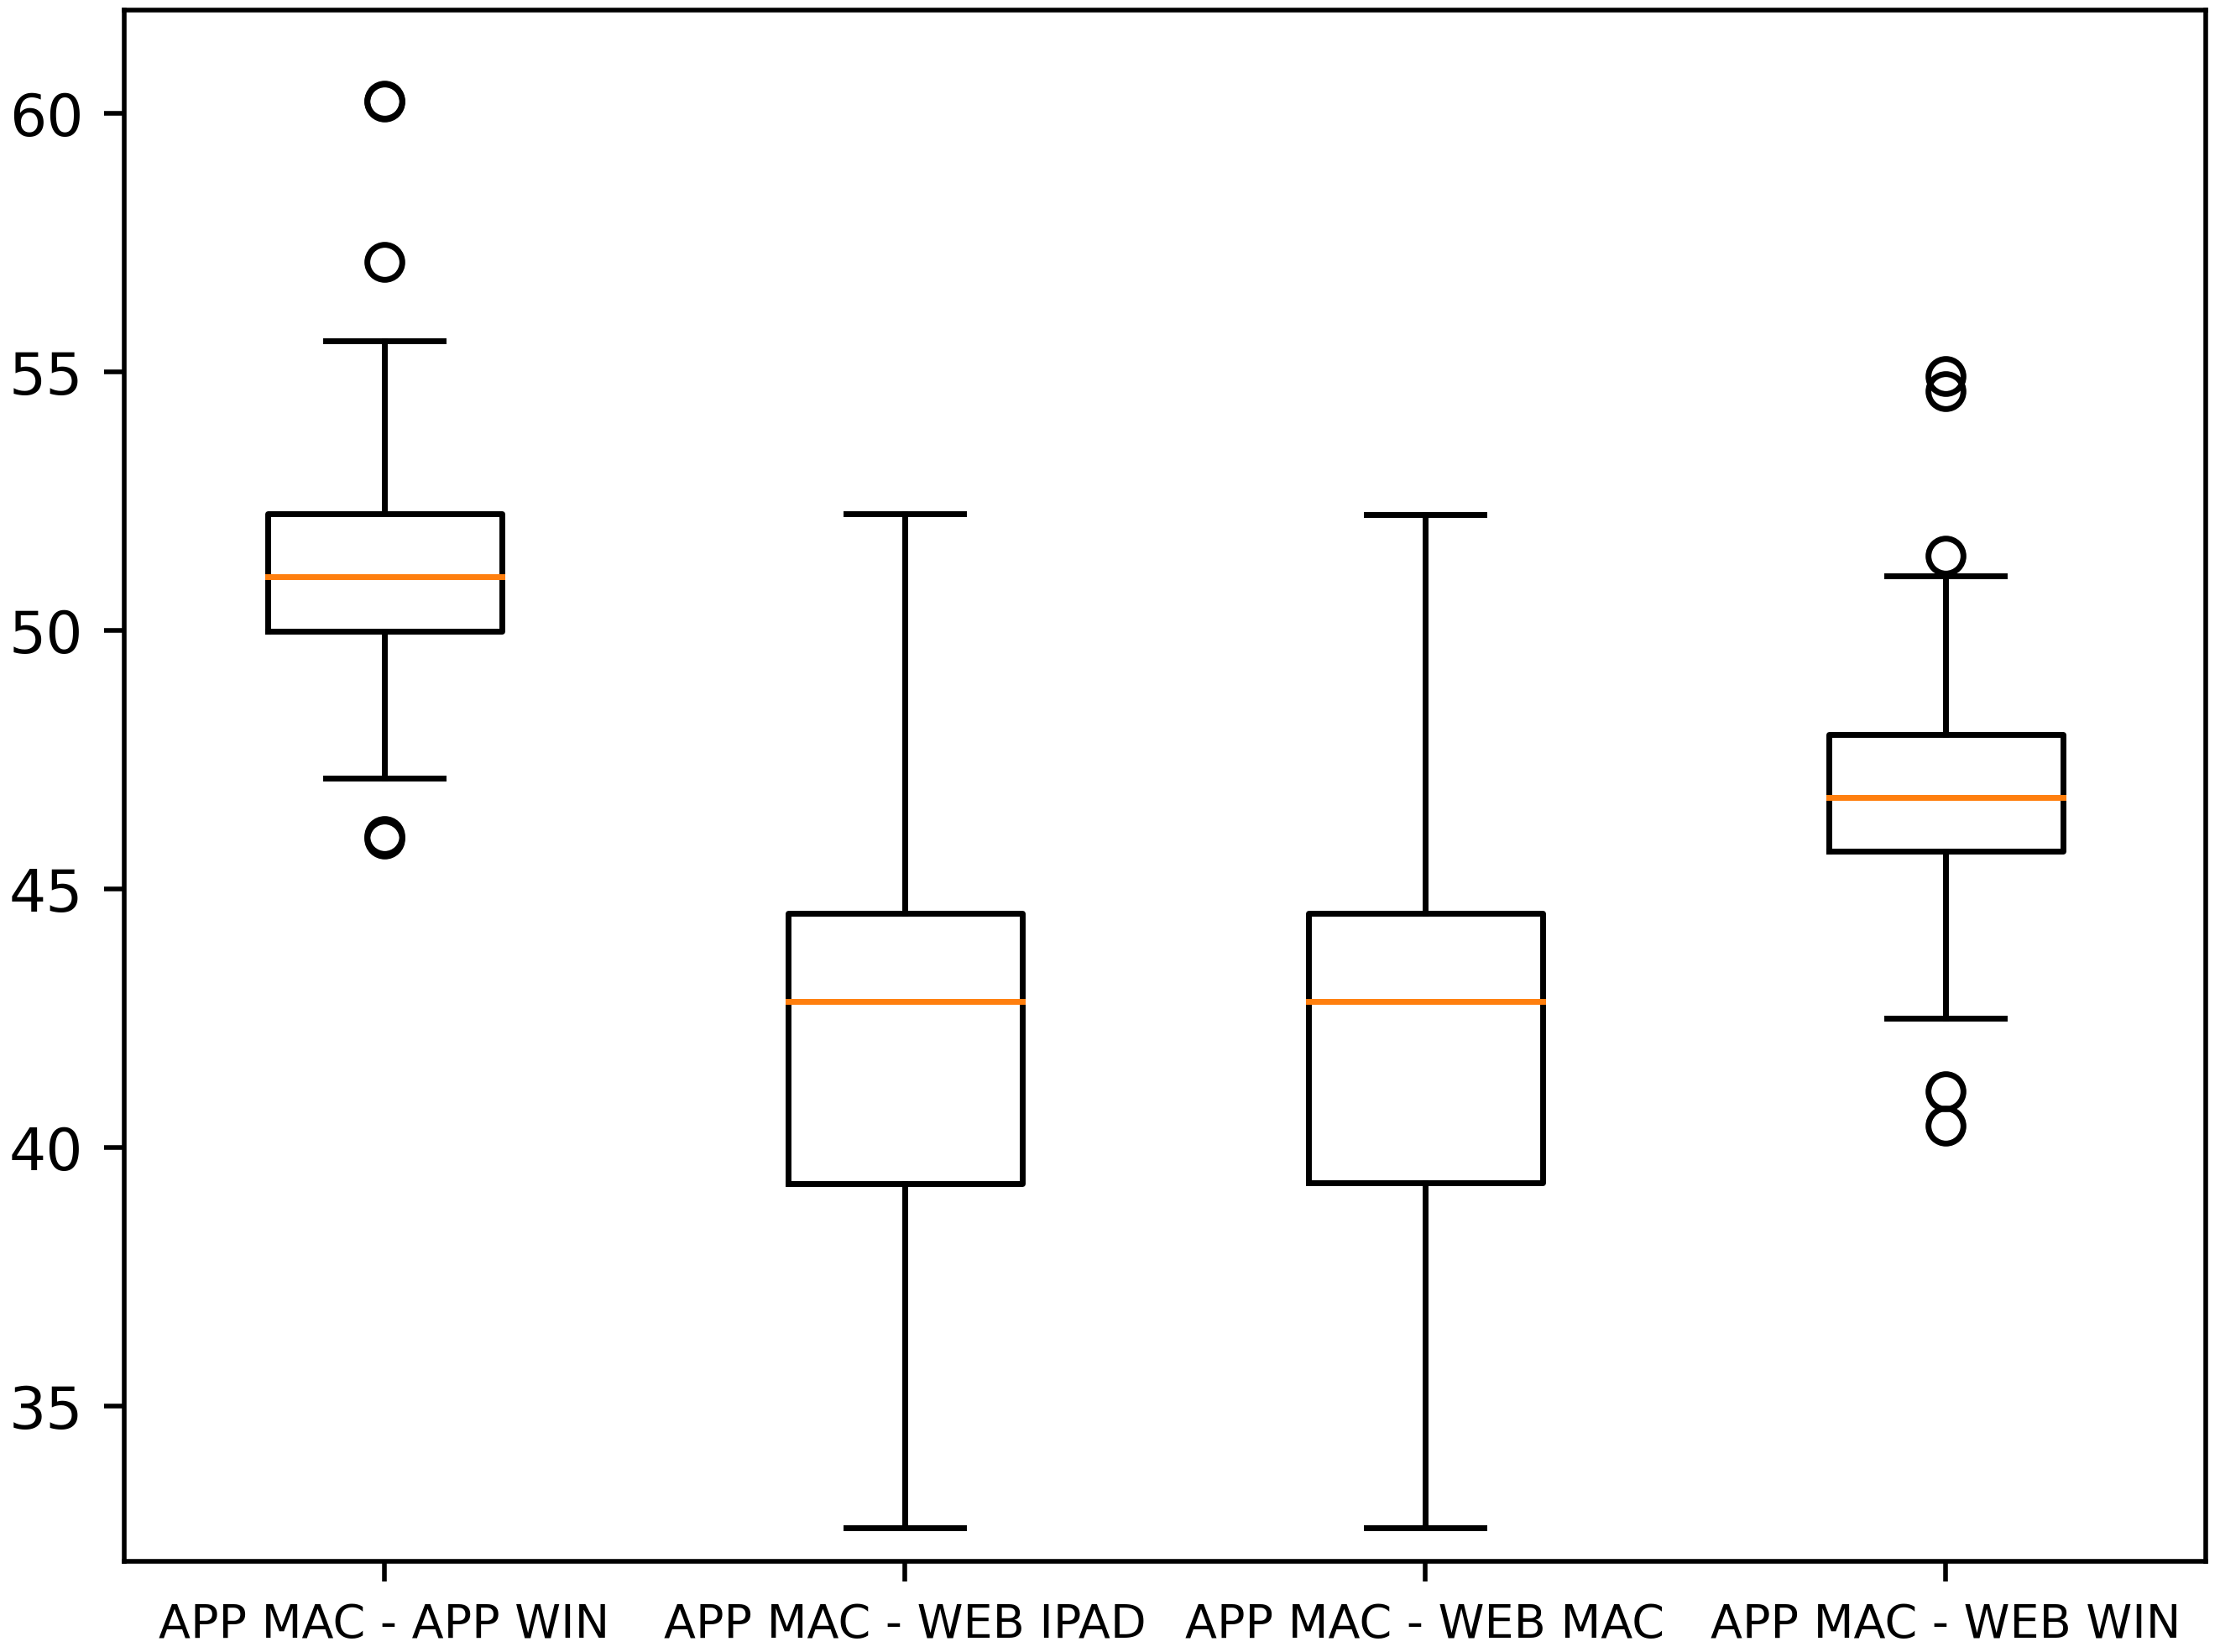
\includegraphics[width=8cm, height=8cm, keepaspectratio]{Immagini/PSNR/Immagine1.png}\hspace{1em}
    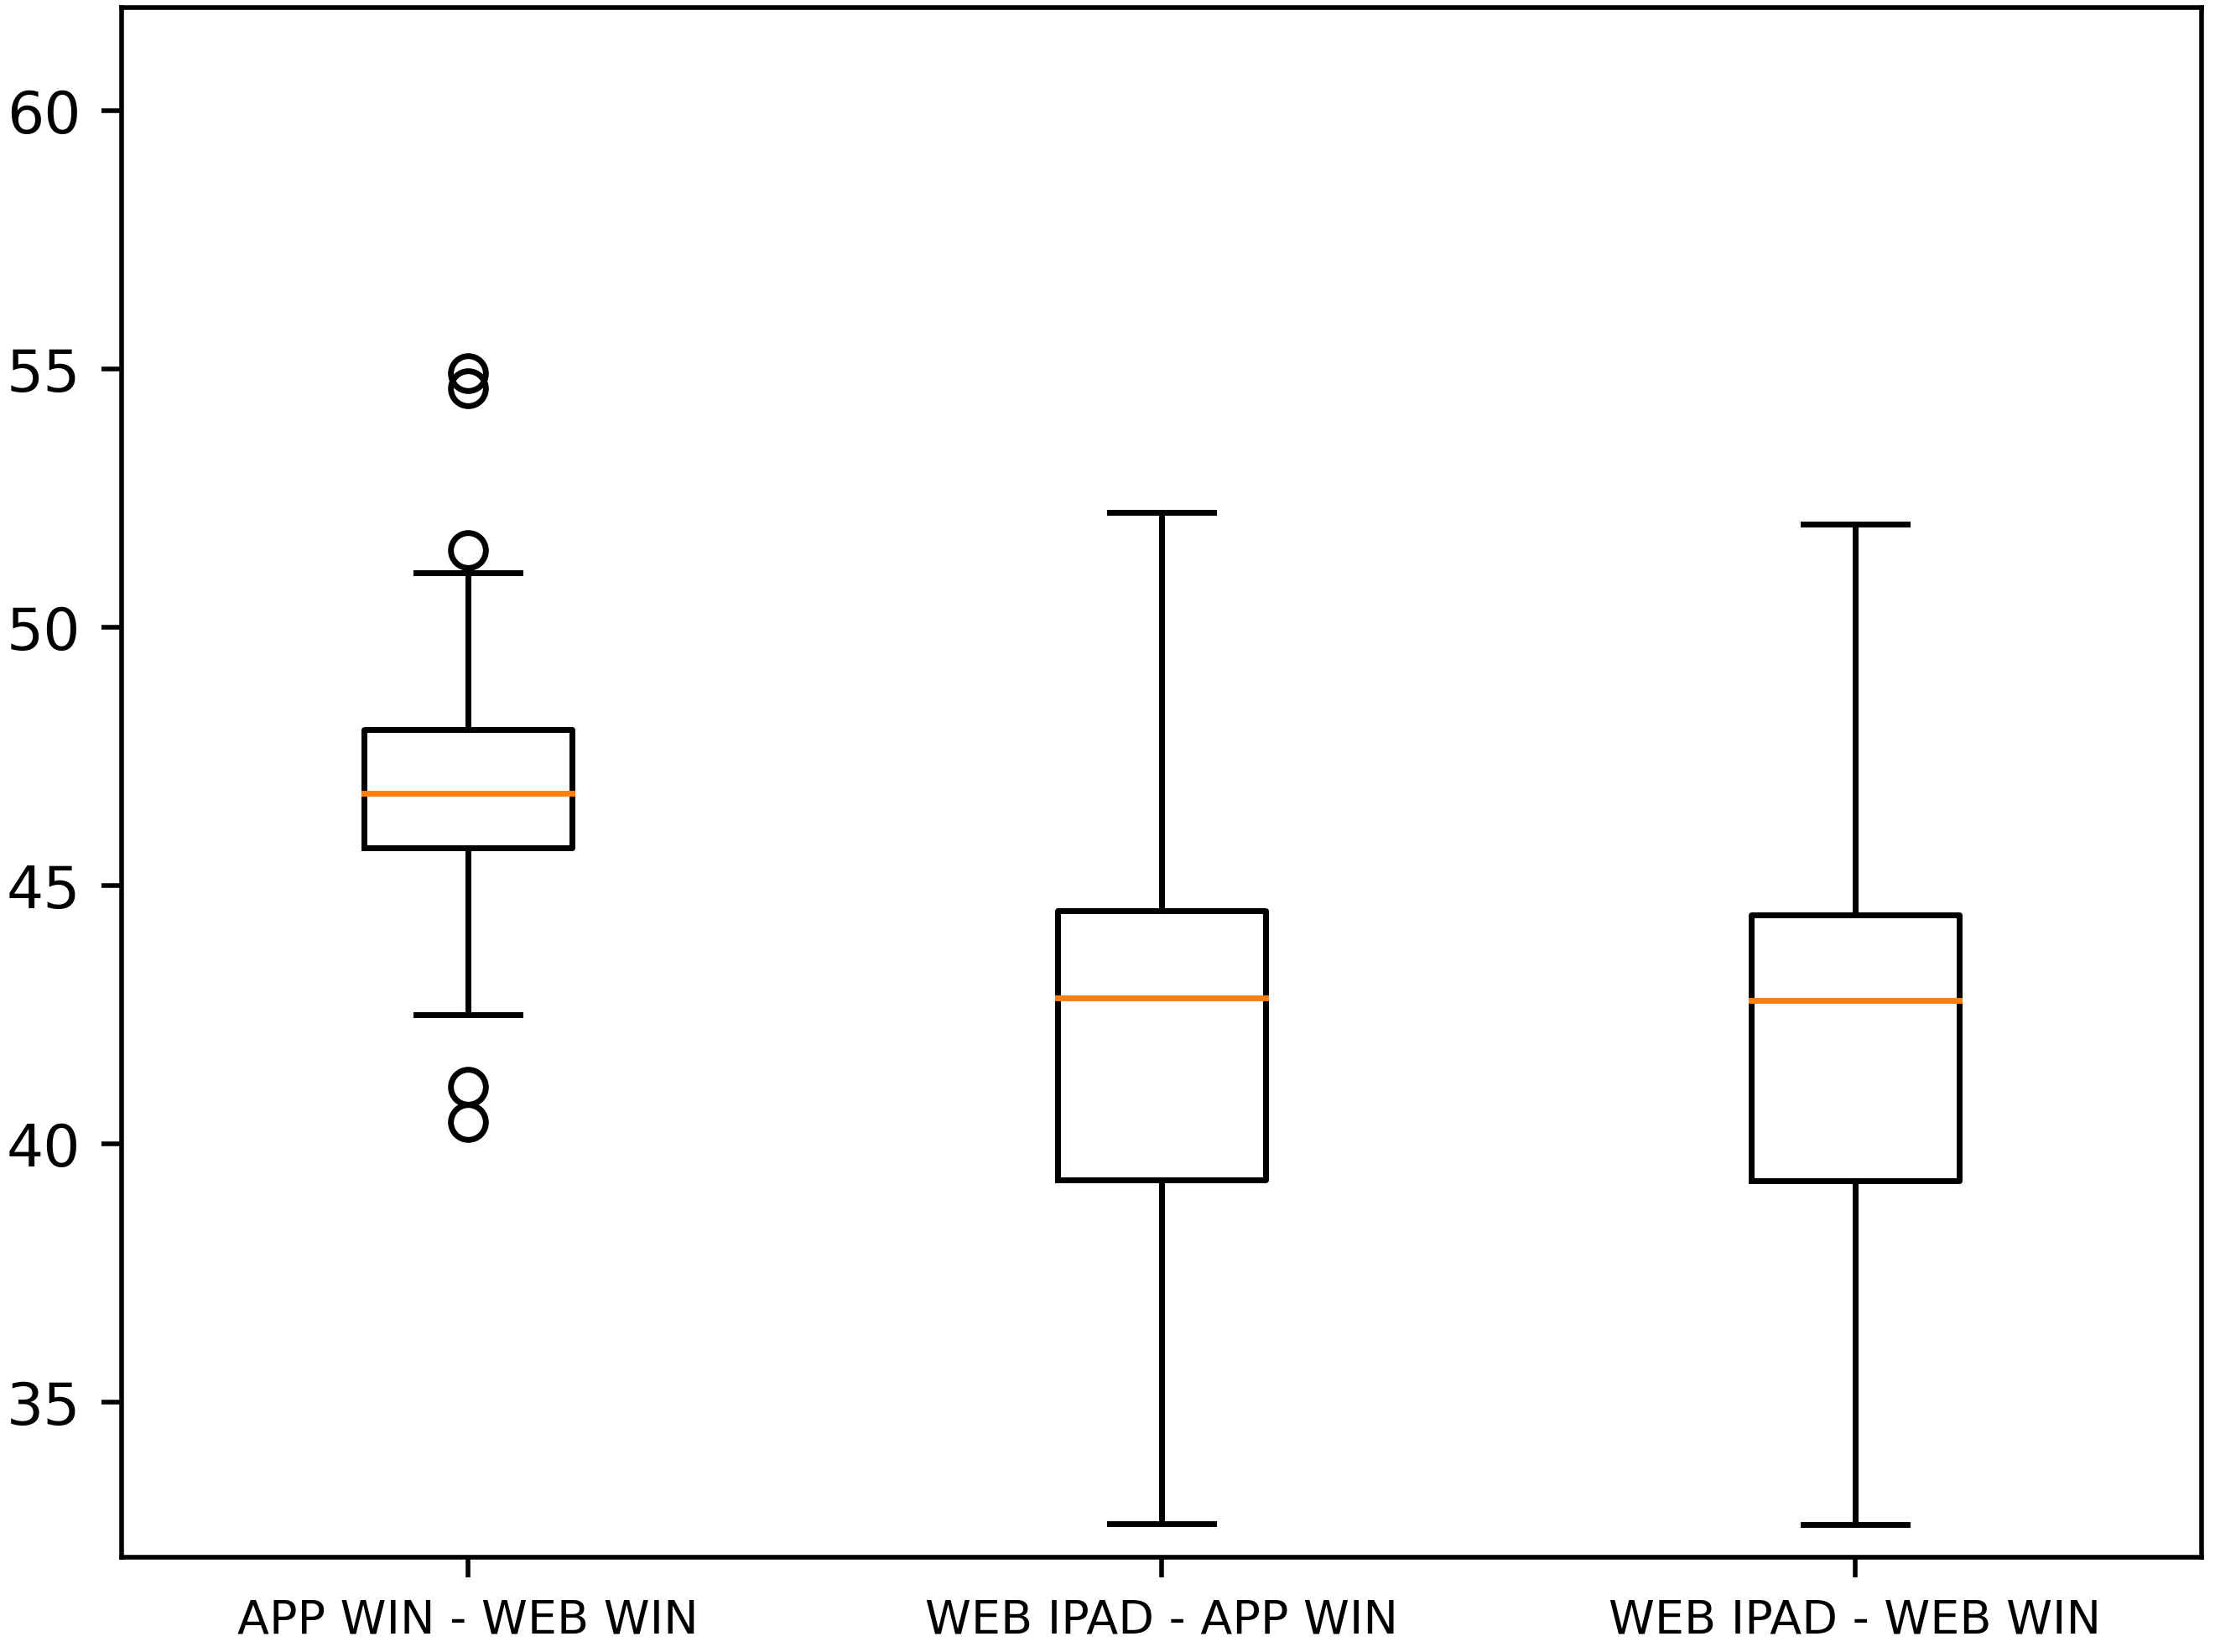
\includegraphics[width=8cm, height=8cm, keepaspectratio]{Immagini/PSNR/Immagine2.png}\\\vspace{1em}
    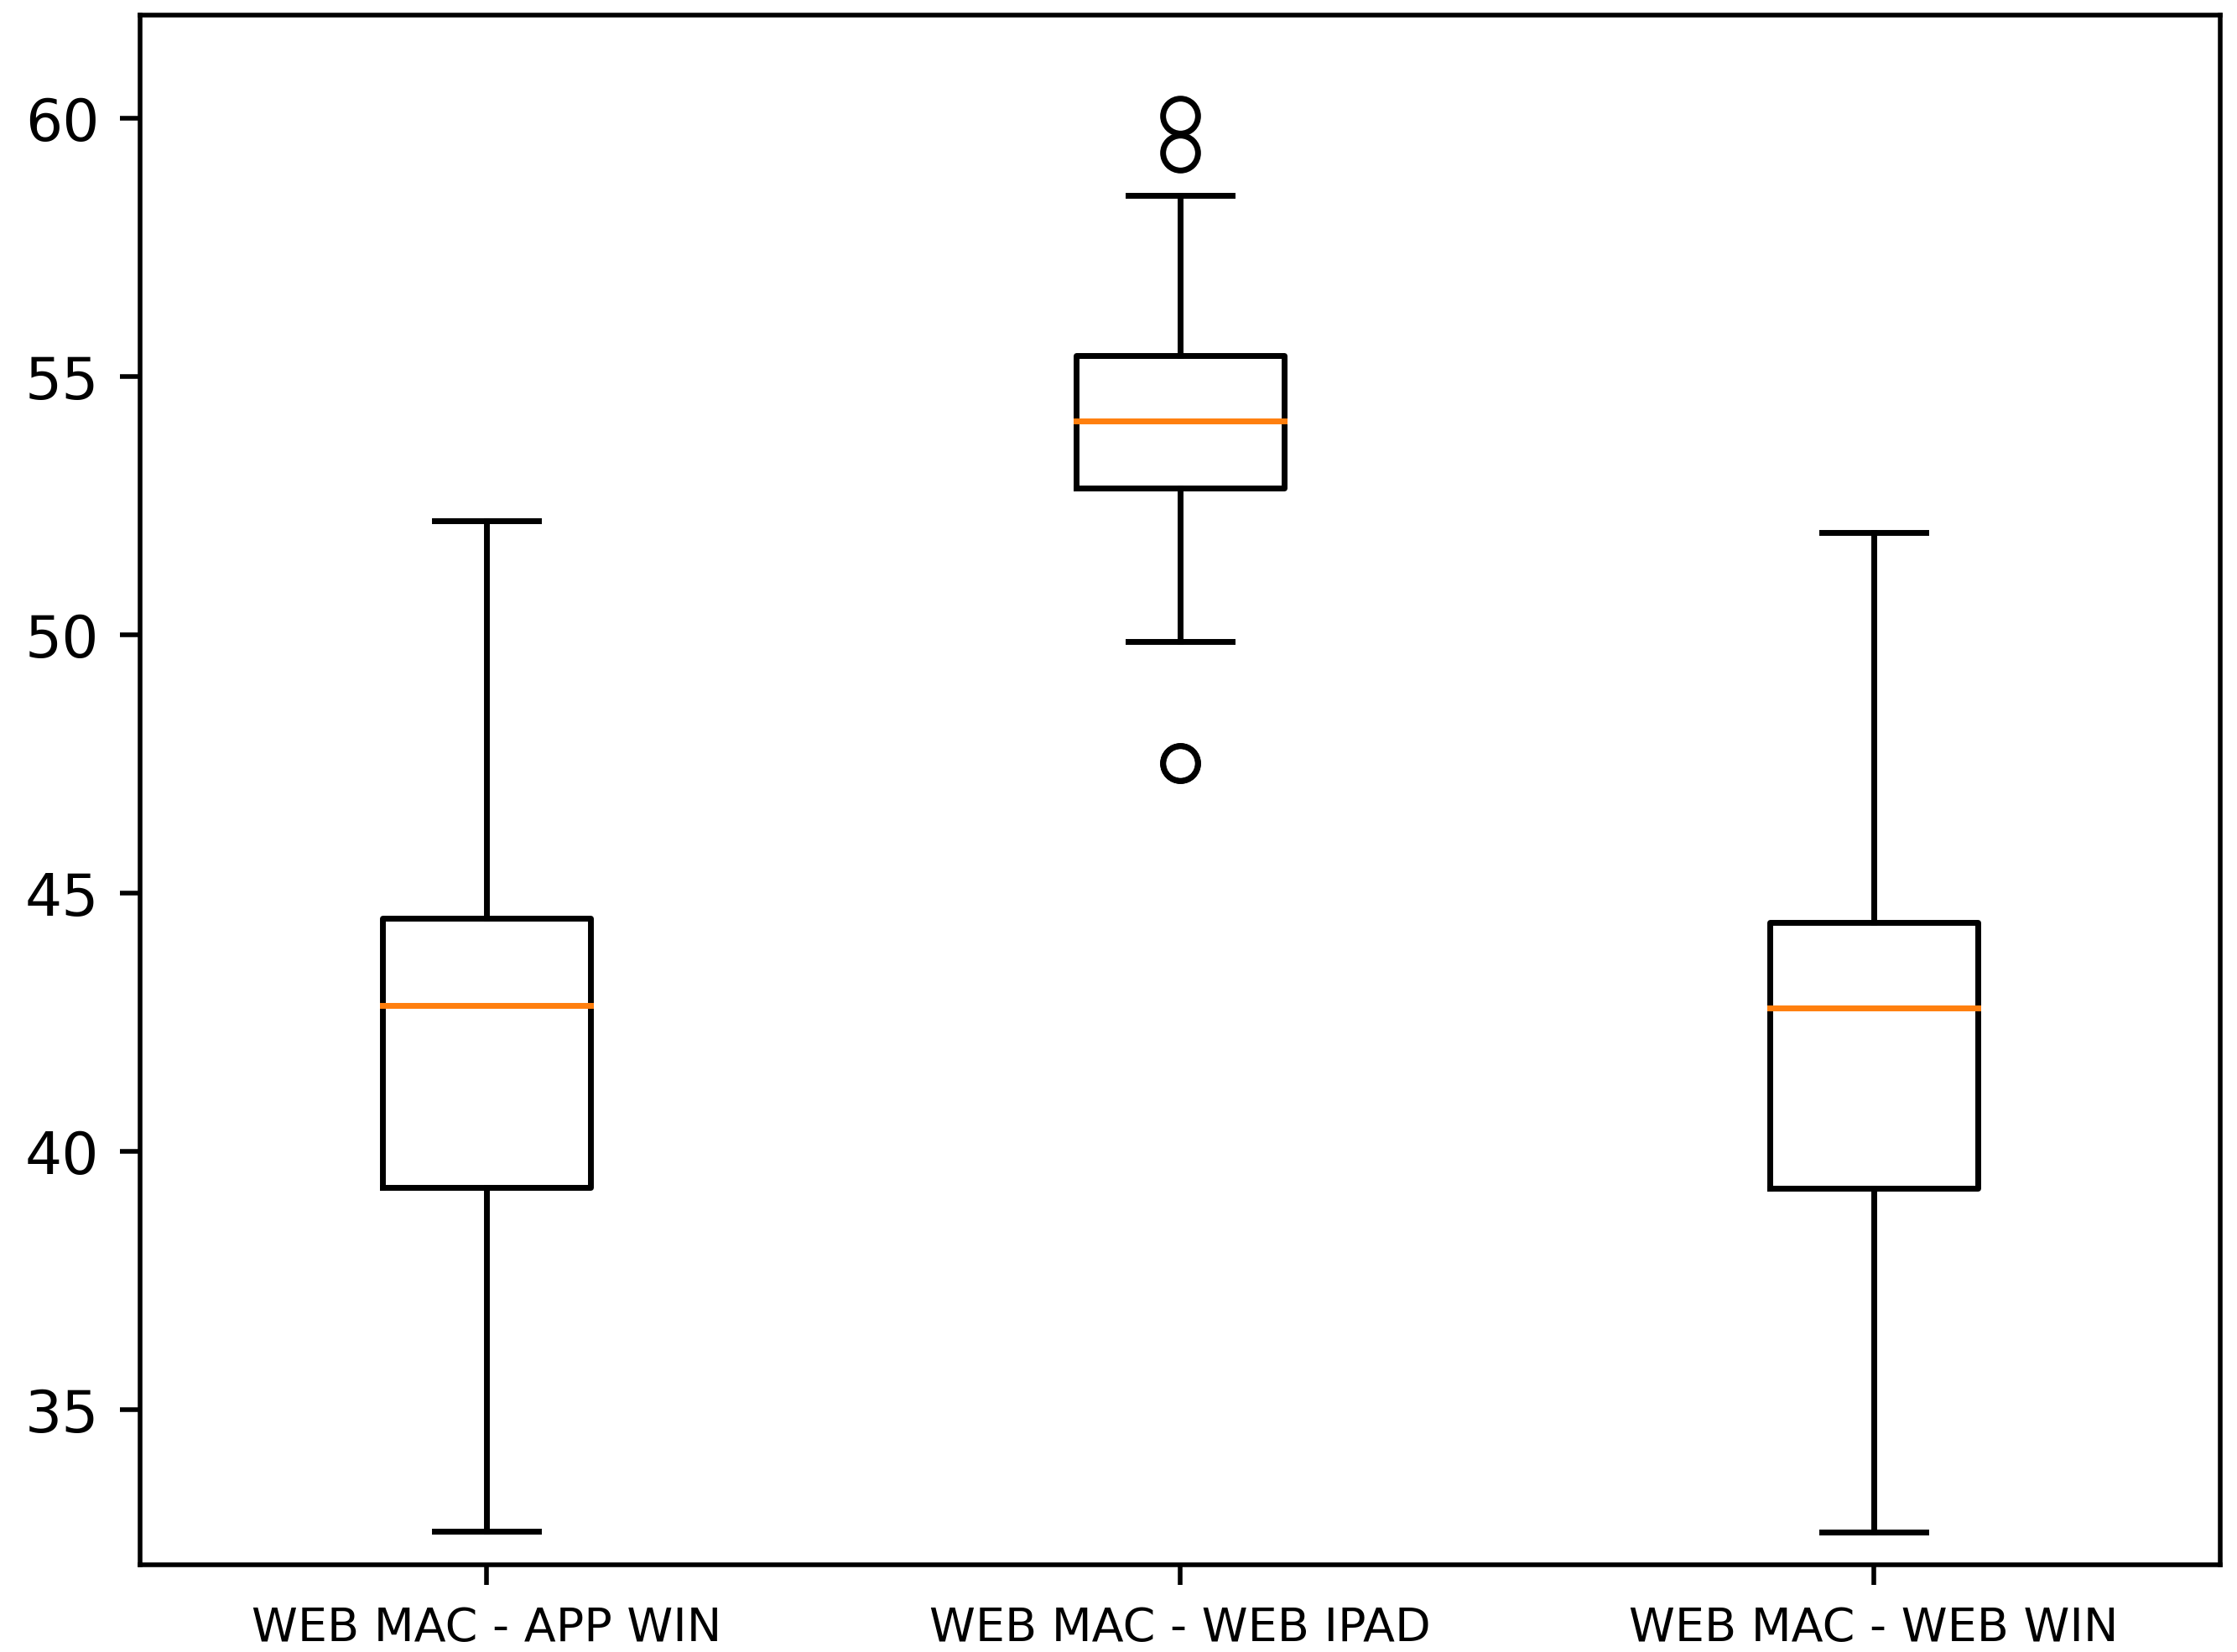
\includegraphics[width=8cm, height=8cm, keepaspectratio]{Immagini/PSNR/Immagine3.png}
    \captionof{figure}{\textit{Boxplot} ricavati dal calcolo del PSNR.}
    \label{fig:psnr_results}
\endgroup

\section{Analisi feature}
\label{sec:feaure_results}
I primi due diagrammi in Fig.~\ref{fig:all_isomap} mostrano la visualizzazione delle \textit{feature} con uno zoom sul cluster centrale in posizione $(0,0)$. A livello macroscopico, i punti che appartengono alla classe \textit{IPHONE} sono ben separati e vanno a formare un insieme di punti distinto dimostrando un'eterogeneità delle \textit{feature} ottenute durante la fase di estrazione. Osservando in dettaglio grazie allo zoom, notiamo che la maggior parte delle classi presenta cluster che sono abbastanza definiti (es., \textit{WEB-WIN}), con due eccezioni: i punti appartenenti alla classe \textit{APP-MAC} sono perfettamente sovrapposti a \textit{APP-WIN} mentre quelli etichettati come \textit{WEB-IPAD} si trovano nella stessa posizione di \textit{WEB-MAC}. Ciò significa che i vettori di \textit{feature} rappresentativi delle immagini hanno gli stessi valori e non possono essere separati. Per questo motivo sono state create due nuove classi:

\begin{itemize}
    \item \textit{APP-DESKTOP}: ottenuta dalla fusione di \textit{APP-MAC} con \textit{APP-WIN}, contiene le immagini condivise tramite l'applicazione desktop di WhatsApp per MacOS e Windows 10;
    
    \item \textit{WEB-SAFARI}: ottenuta dall'unione di \textit{WEB-MAC} con \textit{WEB-IPAD}, include tutte le immagini condivise con il browser Safari tramite tablet e computer.
\end{itemize}

La lista finale delle classi che verranno utilizzate d'ora in poi è quindi composta da: \textit{ANDROID}, \textit{APP-DESKTOP}, \textit{IPHONE}, \textit{WEB-SAFARI} e \textit{WEB-WIN}. A seguito di questa operazione abbiamo eseguito nuovamente la visualizzazione Isomap e i risultati ottenuti sono rappresentati negli ultimi due grafici in Fig.~\ref{fig:all_isomap}. Rispetto a prima, il grado di separazione dei cluster di punti è elevato, fattore che indica una diversità più marcata dei valori delle \textit{feature}. Da ultimo, è stata effettuata la visualizzazione anche per i singoli \textit{quality factor} e, anche se non riportati, i dati ottenuti sono conformi a quanto mostrato finora.\\\\

% \begin{figure}[h!]
%     \centering
%     \subfloat[][]{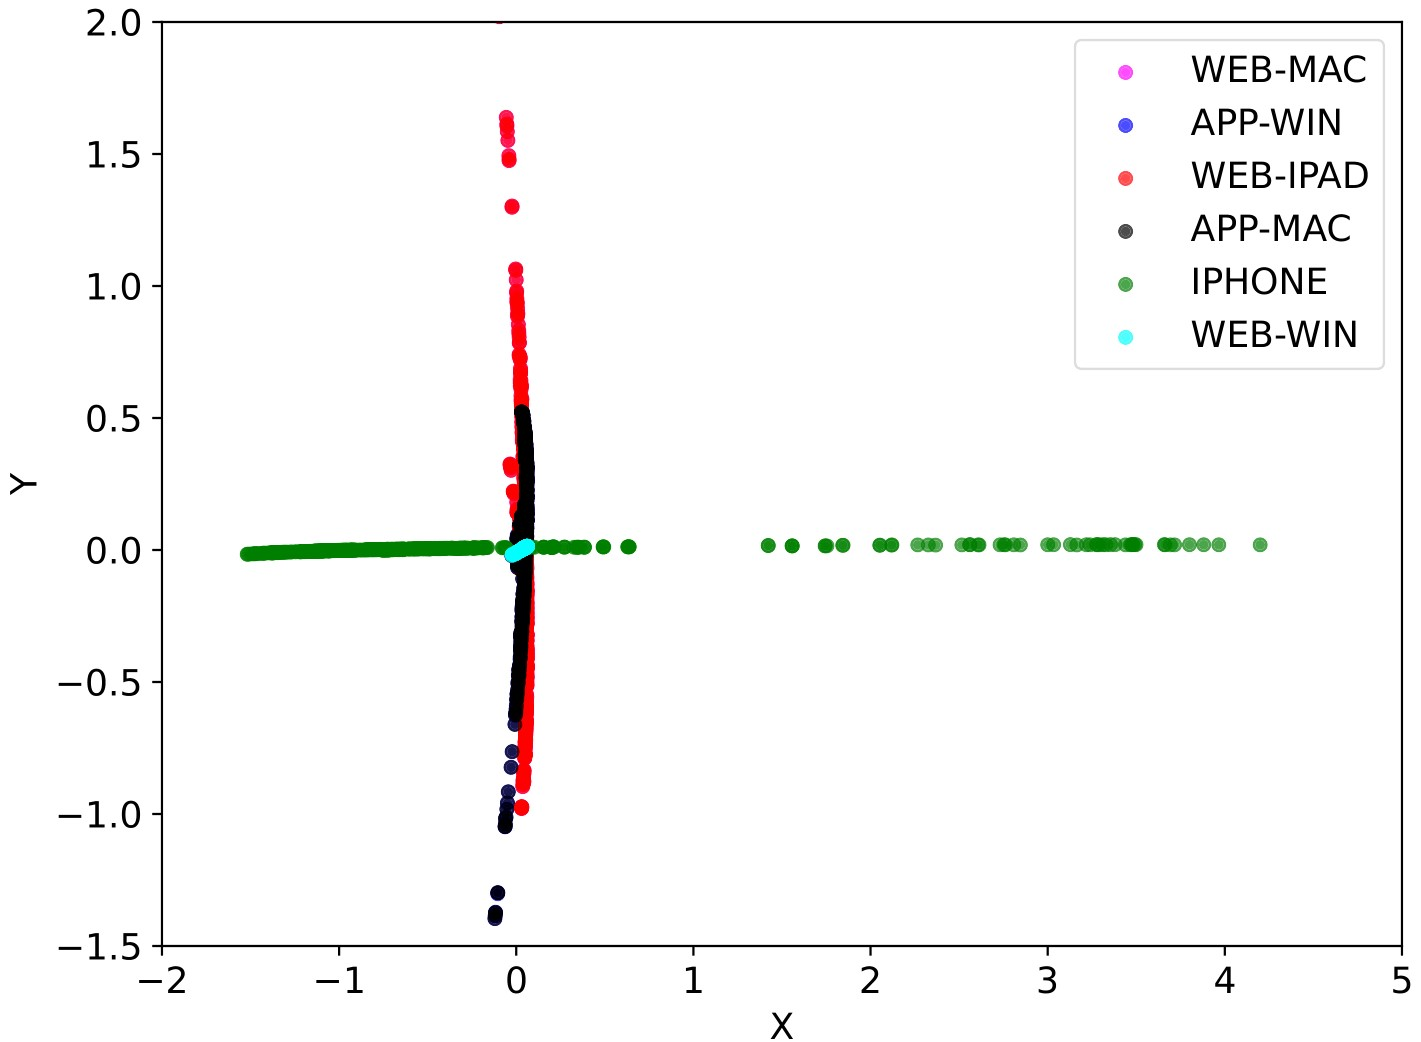
\includegraphics[width=8.5cm, height=8.5cm, keepaspectratio]{Immagini/Isomap/isomap_sep_class.jpg}\label{fig:isomap_sep_class}}
%     \subfloat[][]{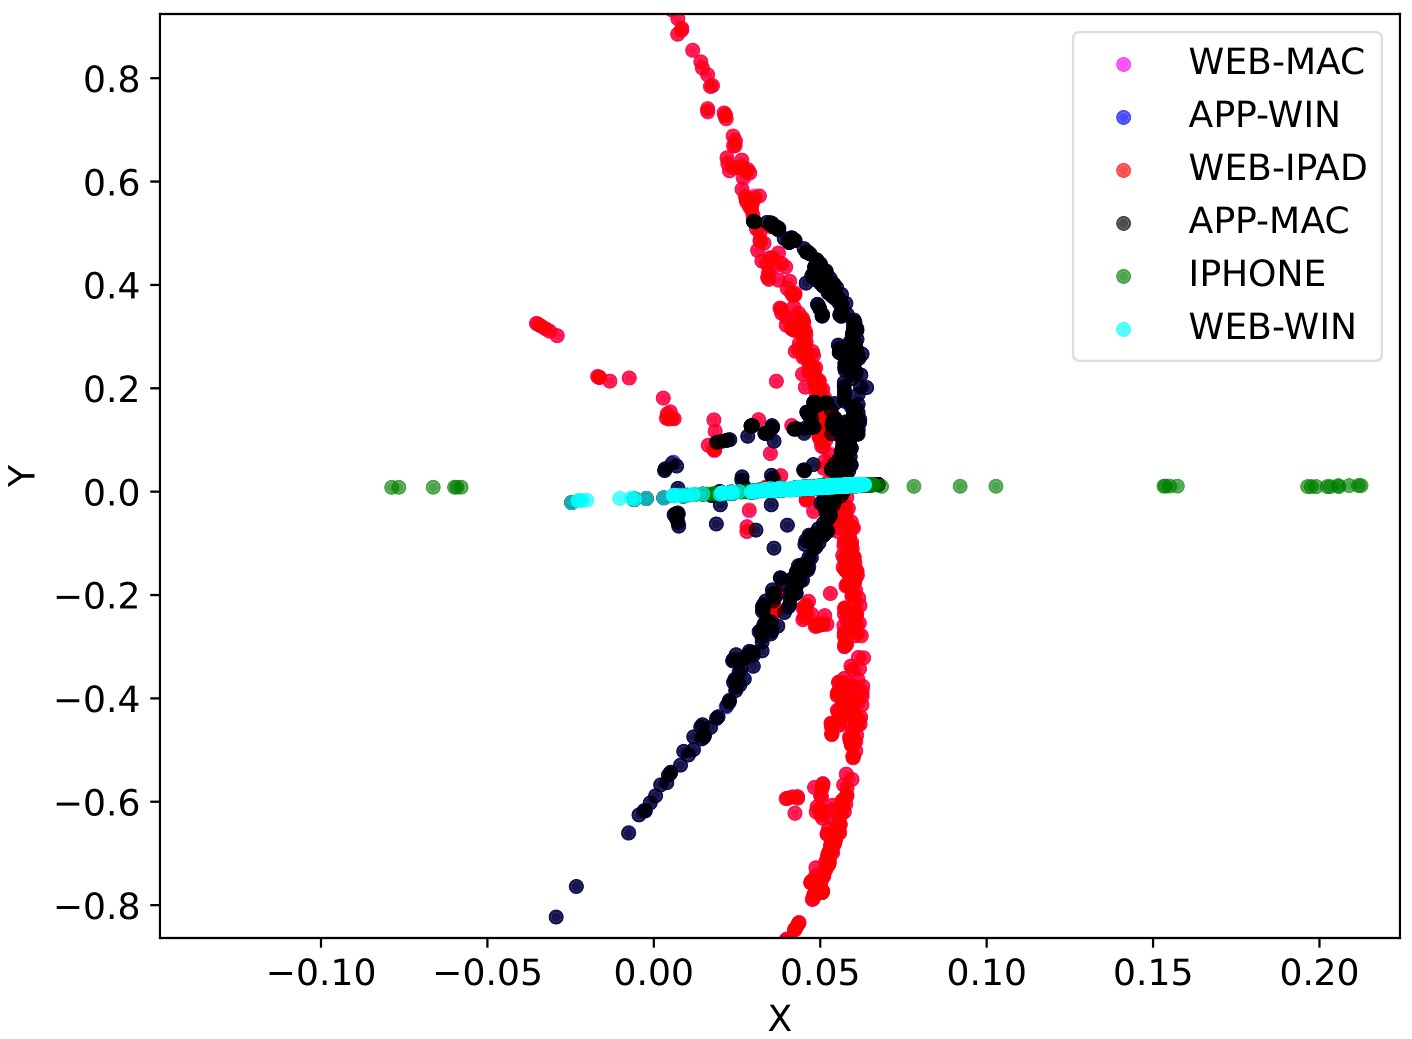
\includegraphics[width=8.5cm, height=8.5cm, keepaspectratio]{Immagini/Isomap/zoom_isomap_sep_class.jpg}\label{fig:isomap_sep_class_zoom}}\\\vspace{1em}
%     \subfloat[][]{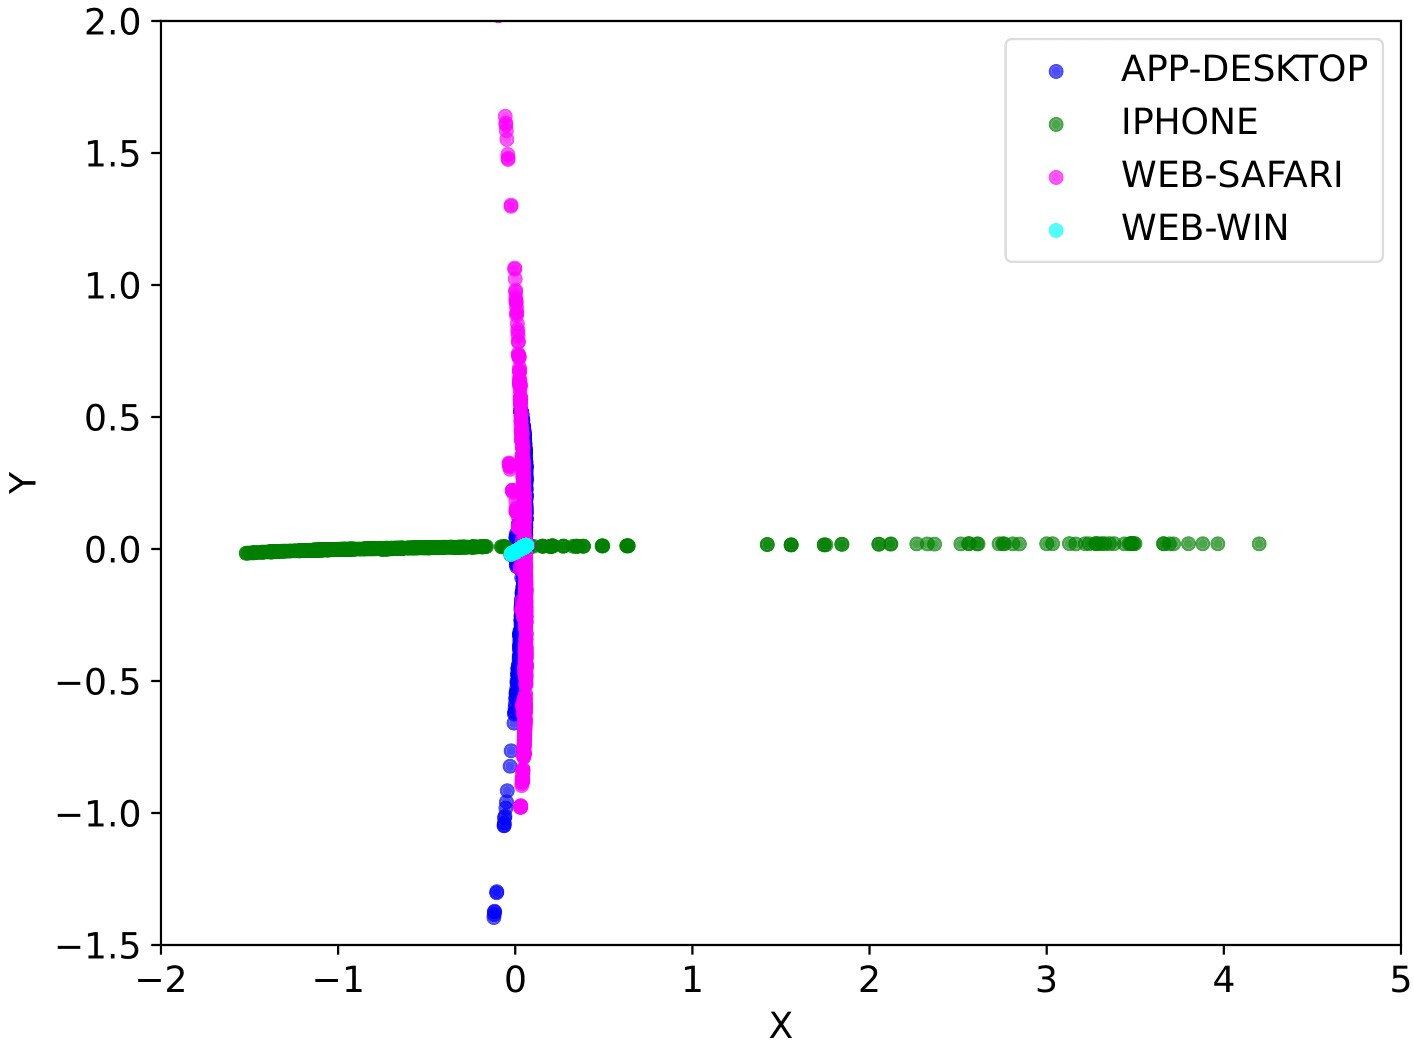
\includegraphics[width=8.5cm, height=8.5cm, keepaspectratio]{Immagini/Isomap/isomap.jpg}\label{fig:isomap}}
%     \subfloat[][]{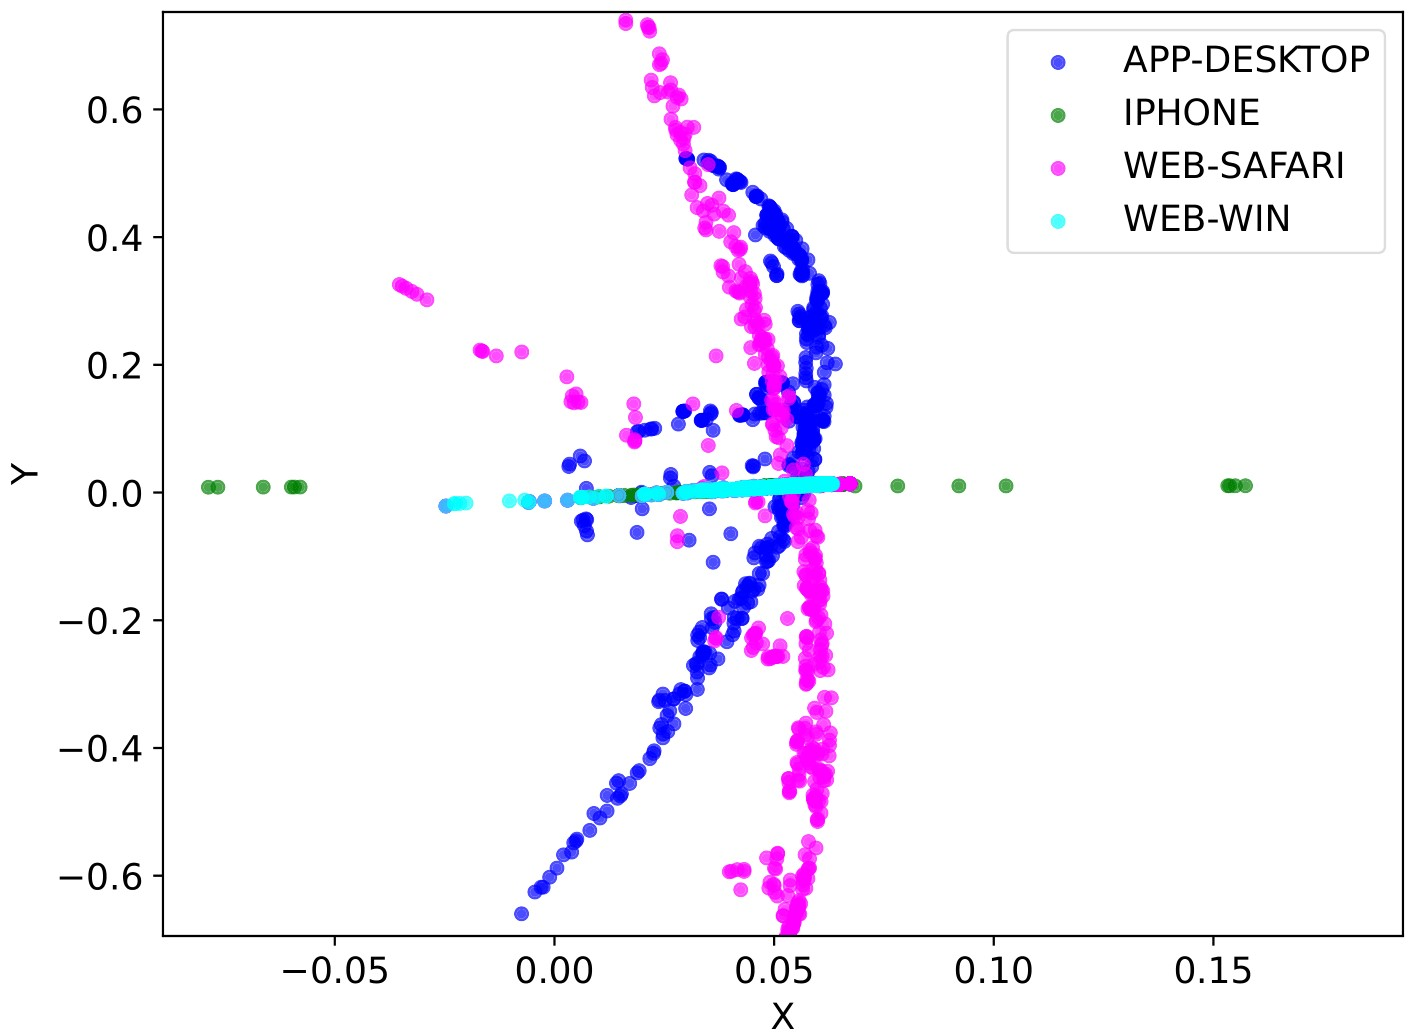
\includegraphics[width=8.5cm, height=8.5cm, keepaspectratio]{Immagini/Isomap/zoom_isomap.jpg}\label{fig:isomap_zoom}}
%     \caption{Rappresentazione Isomap dei vettori di \textit{feature} estratti dalle immagini di SHADE, con una vista complessiva (a, c) e un ingrandimento del cluster vicino all'origine (b, d), sia per le classi separate che dopo la fusione.}
% \end{figure}

\begingroup
    \centering
    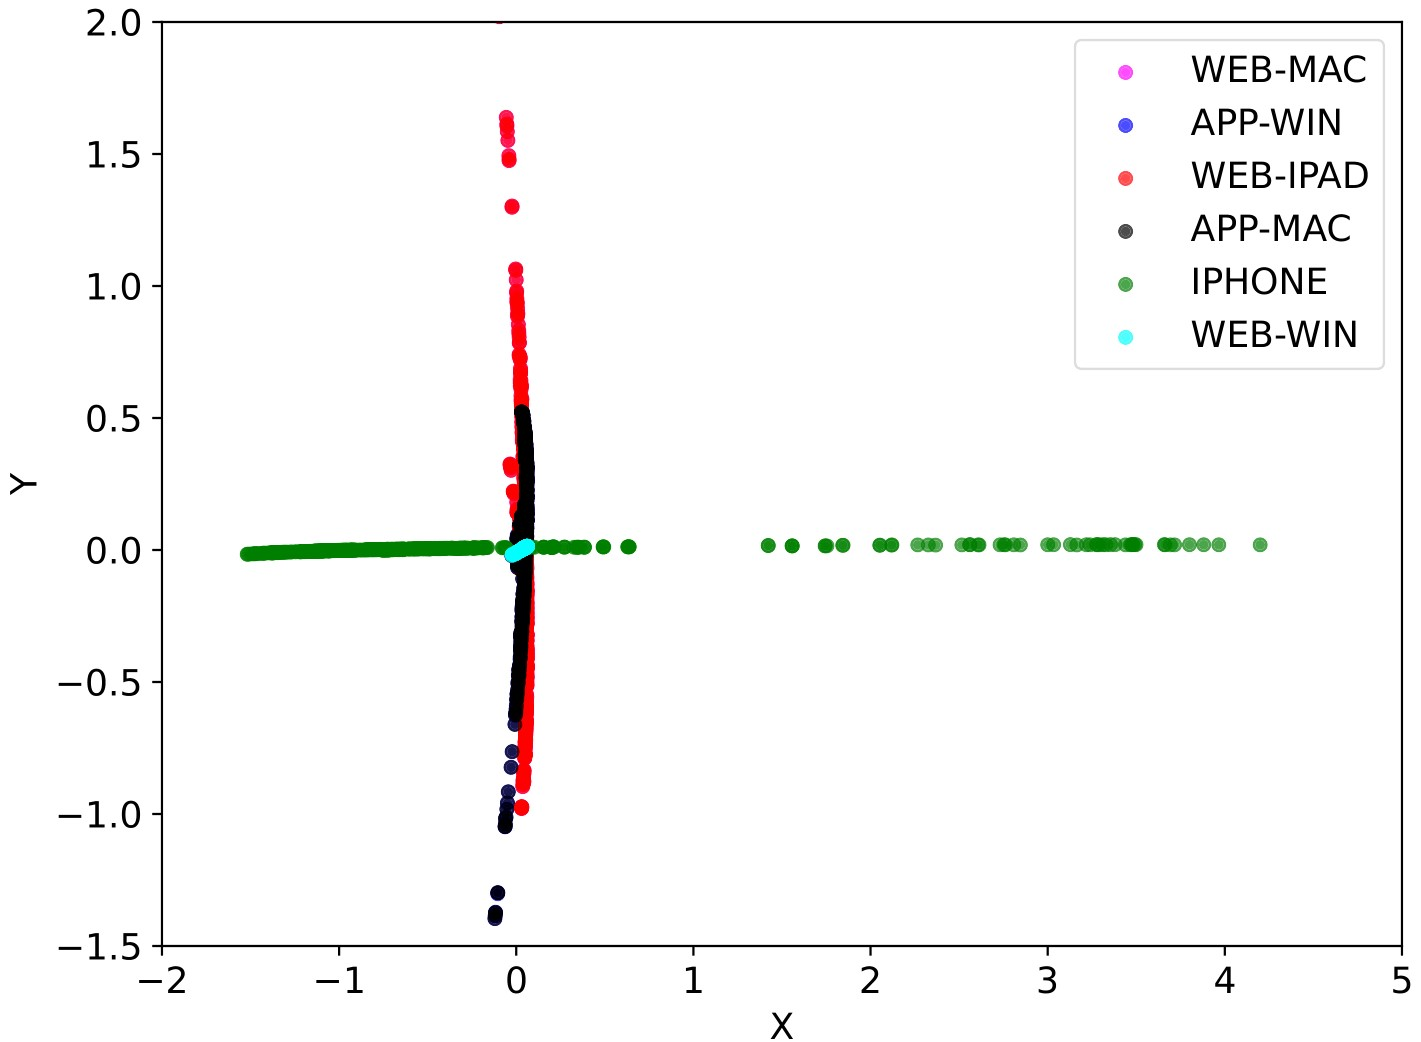
\includegraphics[width=8.5cm, height=8.5cm, keepaspectratio]{Immagini/Isomap/isomap_sep_class.jpg}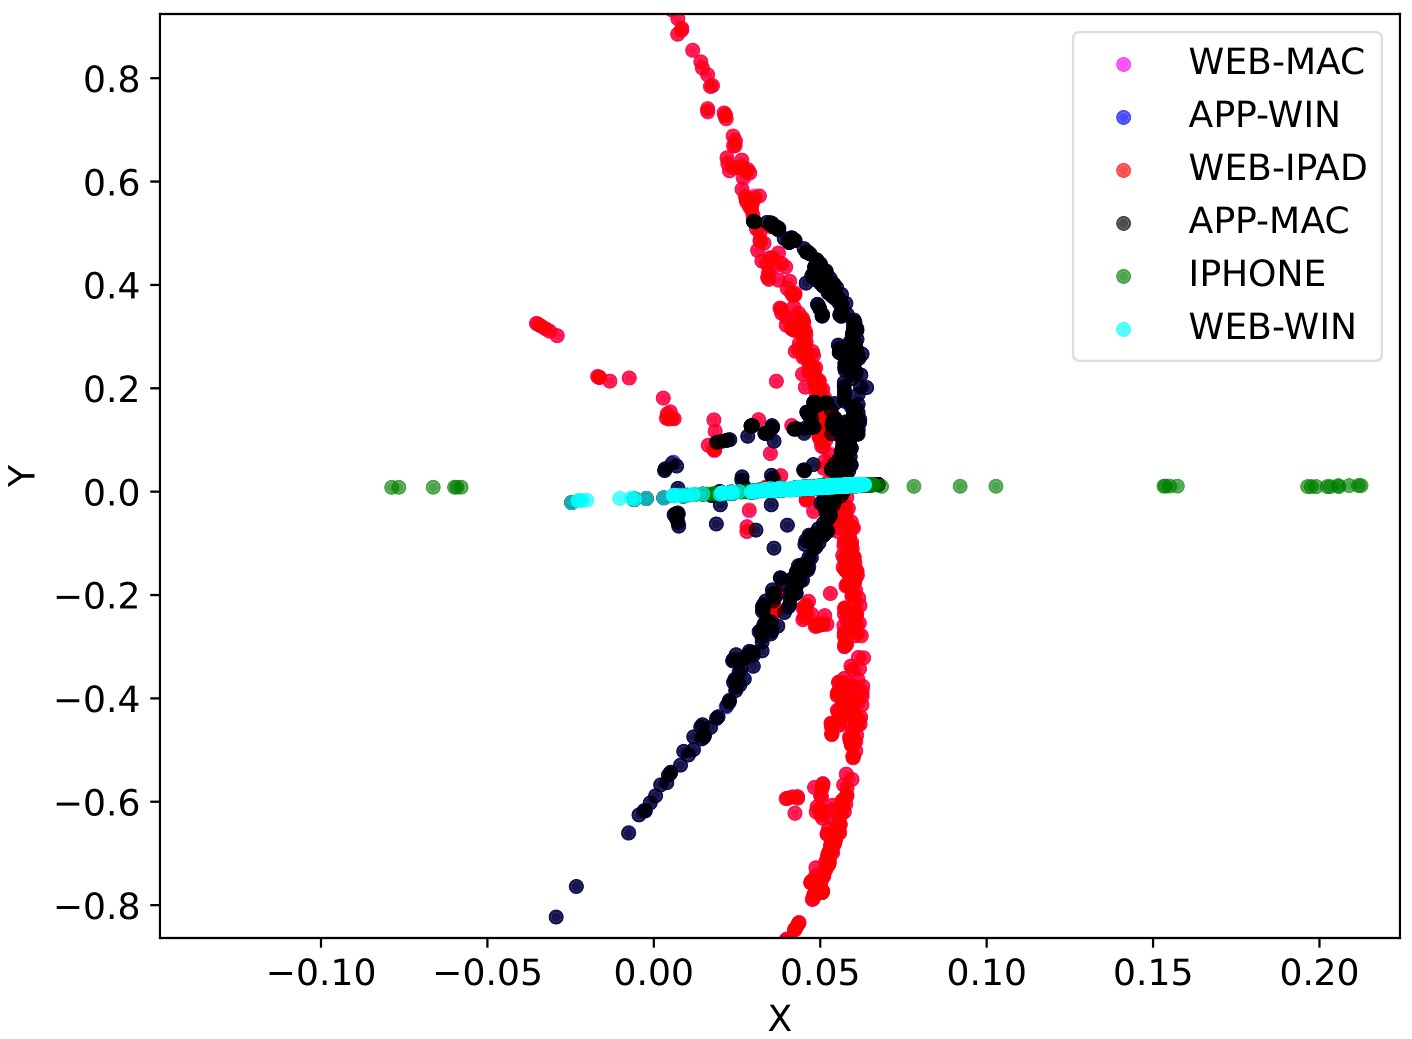
\includegraphics[width=8.5cm, height=8.5cm, keepaspectratio]{Immagini/Isomap/zoom_isomap_sep_class.jpg}\\\vspace{1em}
    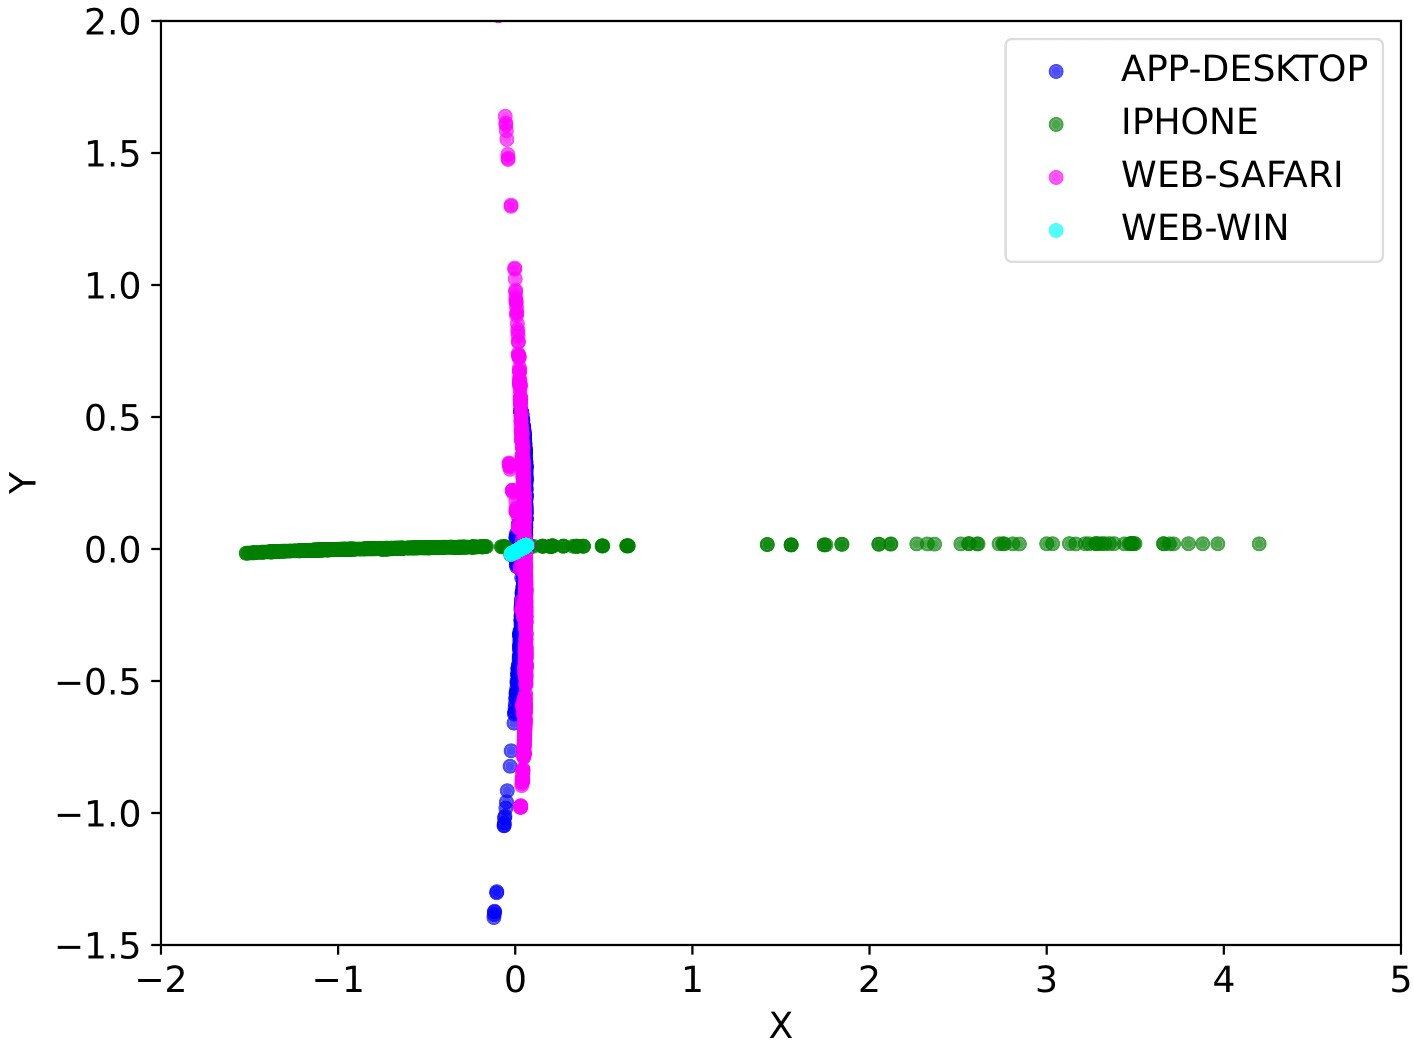
\includegraphics[width=8.5cm, height=8.5cm, keepaspectratio]{Immagini/Isomap/isomap.jpg}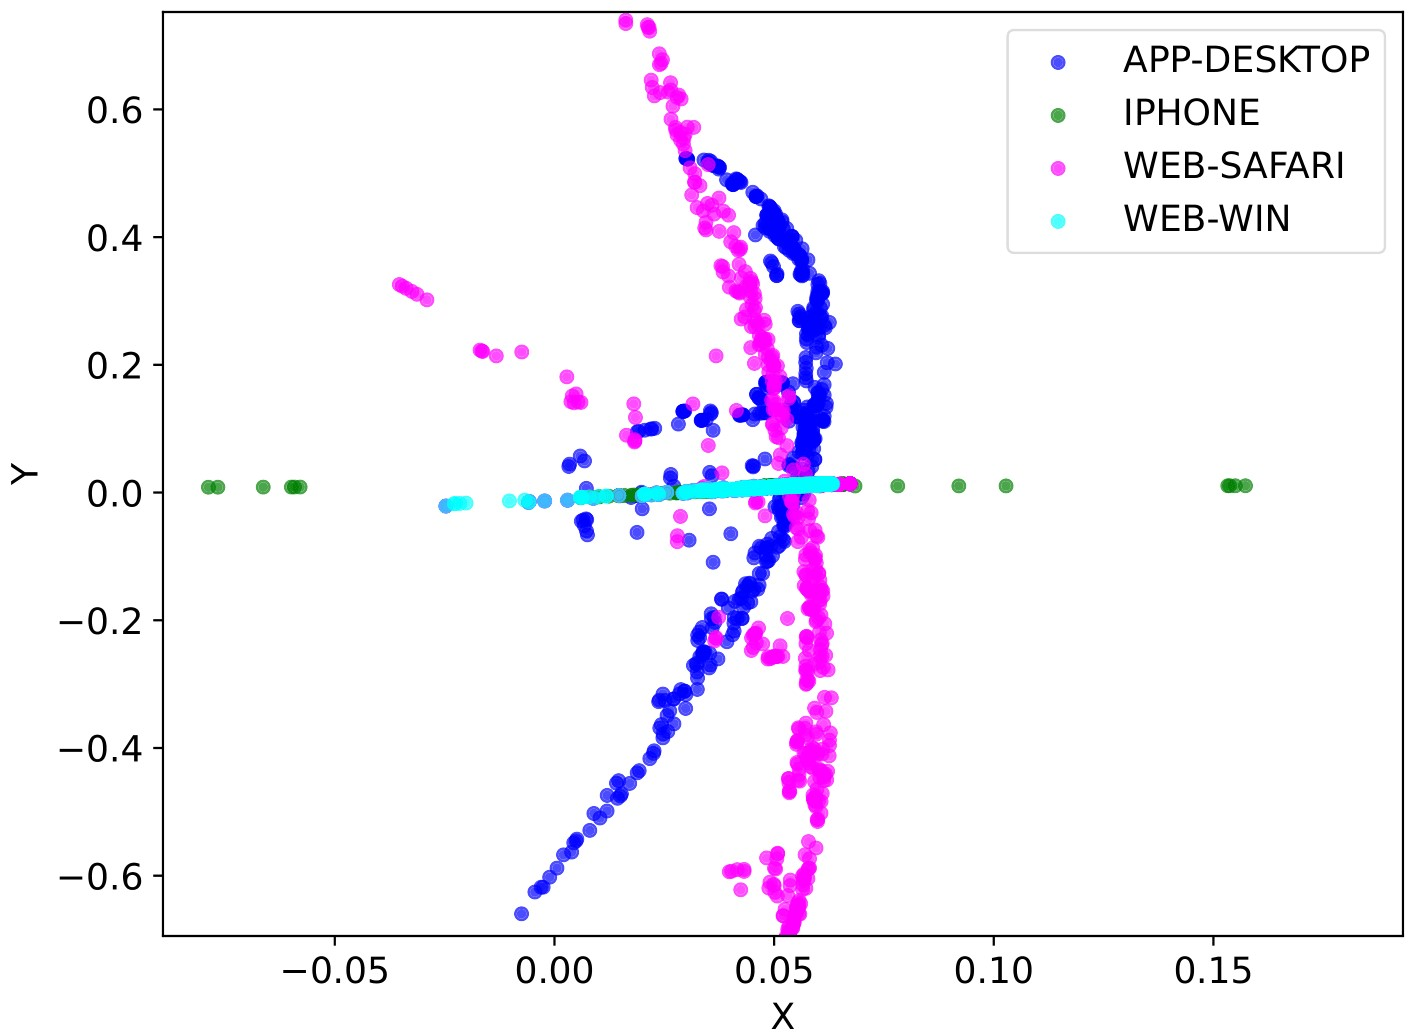
\includegraphics[width=8.5cm, height=8.5cm, keepaspectratio]{Immagini/Isomap/zoom_isomap.jpg}
    \captionof{figure}{Rappresentazione Isomap dei vettori di \textit{feature} estratti dalle immagini di SHADE, con una vista complessiva e un ingrandimento del cluster vicino all'origine, sia per le classi separate che dopo la fusione.}
    \label{fig:all_isomap}
\endgroup

\section{Classificazione}
\label{sec:classification_results}
Terminiamo la presentazione dei risultati mostrando le \textit{confusion matrix} (Fig.~\ref{fig:class}) ottenute dalla classificazione. Ogni cella $(i,j)$ di queste tabelle, con $i$ come riga e $j$ come colonna, contiene il numero di immagini predette con classe $j$ rispetto al metodo di condivisione $i$. Il numero ottenuto è stato poi normalizzato in modo da essere compreso tra 0 e 1. Il dato più rilevante riscontrato è che la classe \textit{IPHONE} viene identificata correttamente nel 100\% dei casi, confermando quanto era emerso dalla visualizzazione Isomap. Per quanto riguarda le rimanenti classi, le performance ottenute sono soddisfacenti con valori di accuratezza che variano tra il 69\% e il 73\% nel caso di \textit{random forest} e tra il 72\% e il 78\% nel caso di \textit{support vector machine}. La seguente tabella mostra per ogni classe considerata quella con più falsi positivi.

\begin{center}
    \begin{tabular}{llll}
    \hline
    \\[-1em]
    \textbf{metodo} & \textbf{classe} & \textbf{classe con più falsi positivi} & \textbf{N. occorrenze} \\[-1em]\\
    \hline
    \\[-1em]
    \multirow{5}{4em}{\textbf{RF}} & \textit{APP-DESKTOP} & \textit{ANDROID} & 234 \\[-1em]\\
    & \textit{IPHONE} & - & - \\[-1em]\\
    & \textit{WEB-SAFARI} & \textit{ANDROID} & 252 \\[-1em]\\
    & \textit{WEB-WIN} & \textit{ANDROID} & 108 \\[-1em]\\
    & \textit{ANDROID} & \textit{APP-DESKTOP} & 117 \\[-1em]\\
    \hline
    \\[-1em]
    \multirow{5}{4em}{\textbf{SVM}} & \textit{APP-DESKTOP} & \textit{WEB-SAFARI} & 234 \\[-1em]\\
    & \textit{IPHONE} & - & - \\[-1em]\\
    & \textit{WEB-SAFARI} & \textit{APP-DESKTOP } & 180 \\[-1em]\\
    & \textit{WEB-WIN} & \textit{WEB-SAFARI} & 99 \\[-1em]\\
    & \textit{ANDROID} & \textit{WEB-SAFARI} & 108 \\[-1em]\\
    \hline
    \end{tabular}
\end{center}

Nonostante le performance non raggiungano il livello di \textit{IPHONE}, le classi analizzate sono comunque ben separabili e possono essere identificate abbastanza facilmente. La classificazione delle immagini in base al \textit{quality factor} (Fig.~\ref{fig:class_QF_RF},~\ref{fig:class_QF_SVM}) ha dato risultati simili sia per RF che per SVM. Abbiamo notato però che in quest'ultimo caso il livello di accuratezza è minore per alcune classi ma più elevato per altre.\\

\begingroup
    \centering
    \subfloat[][]{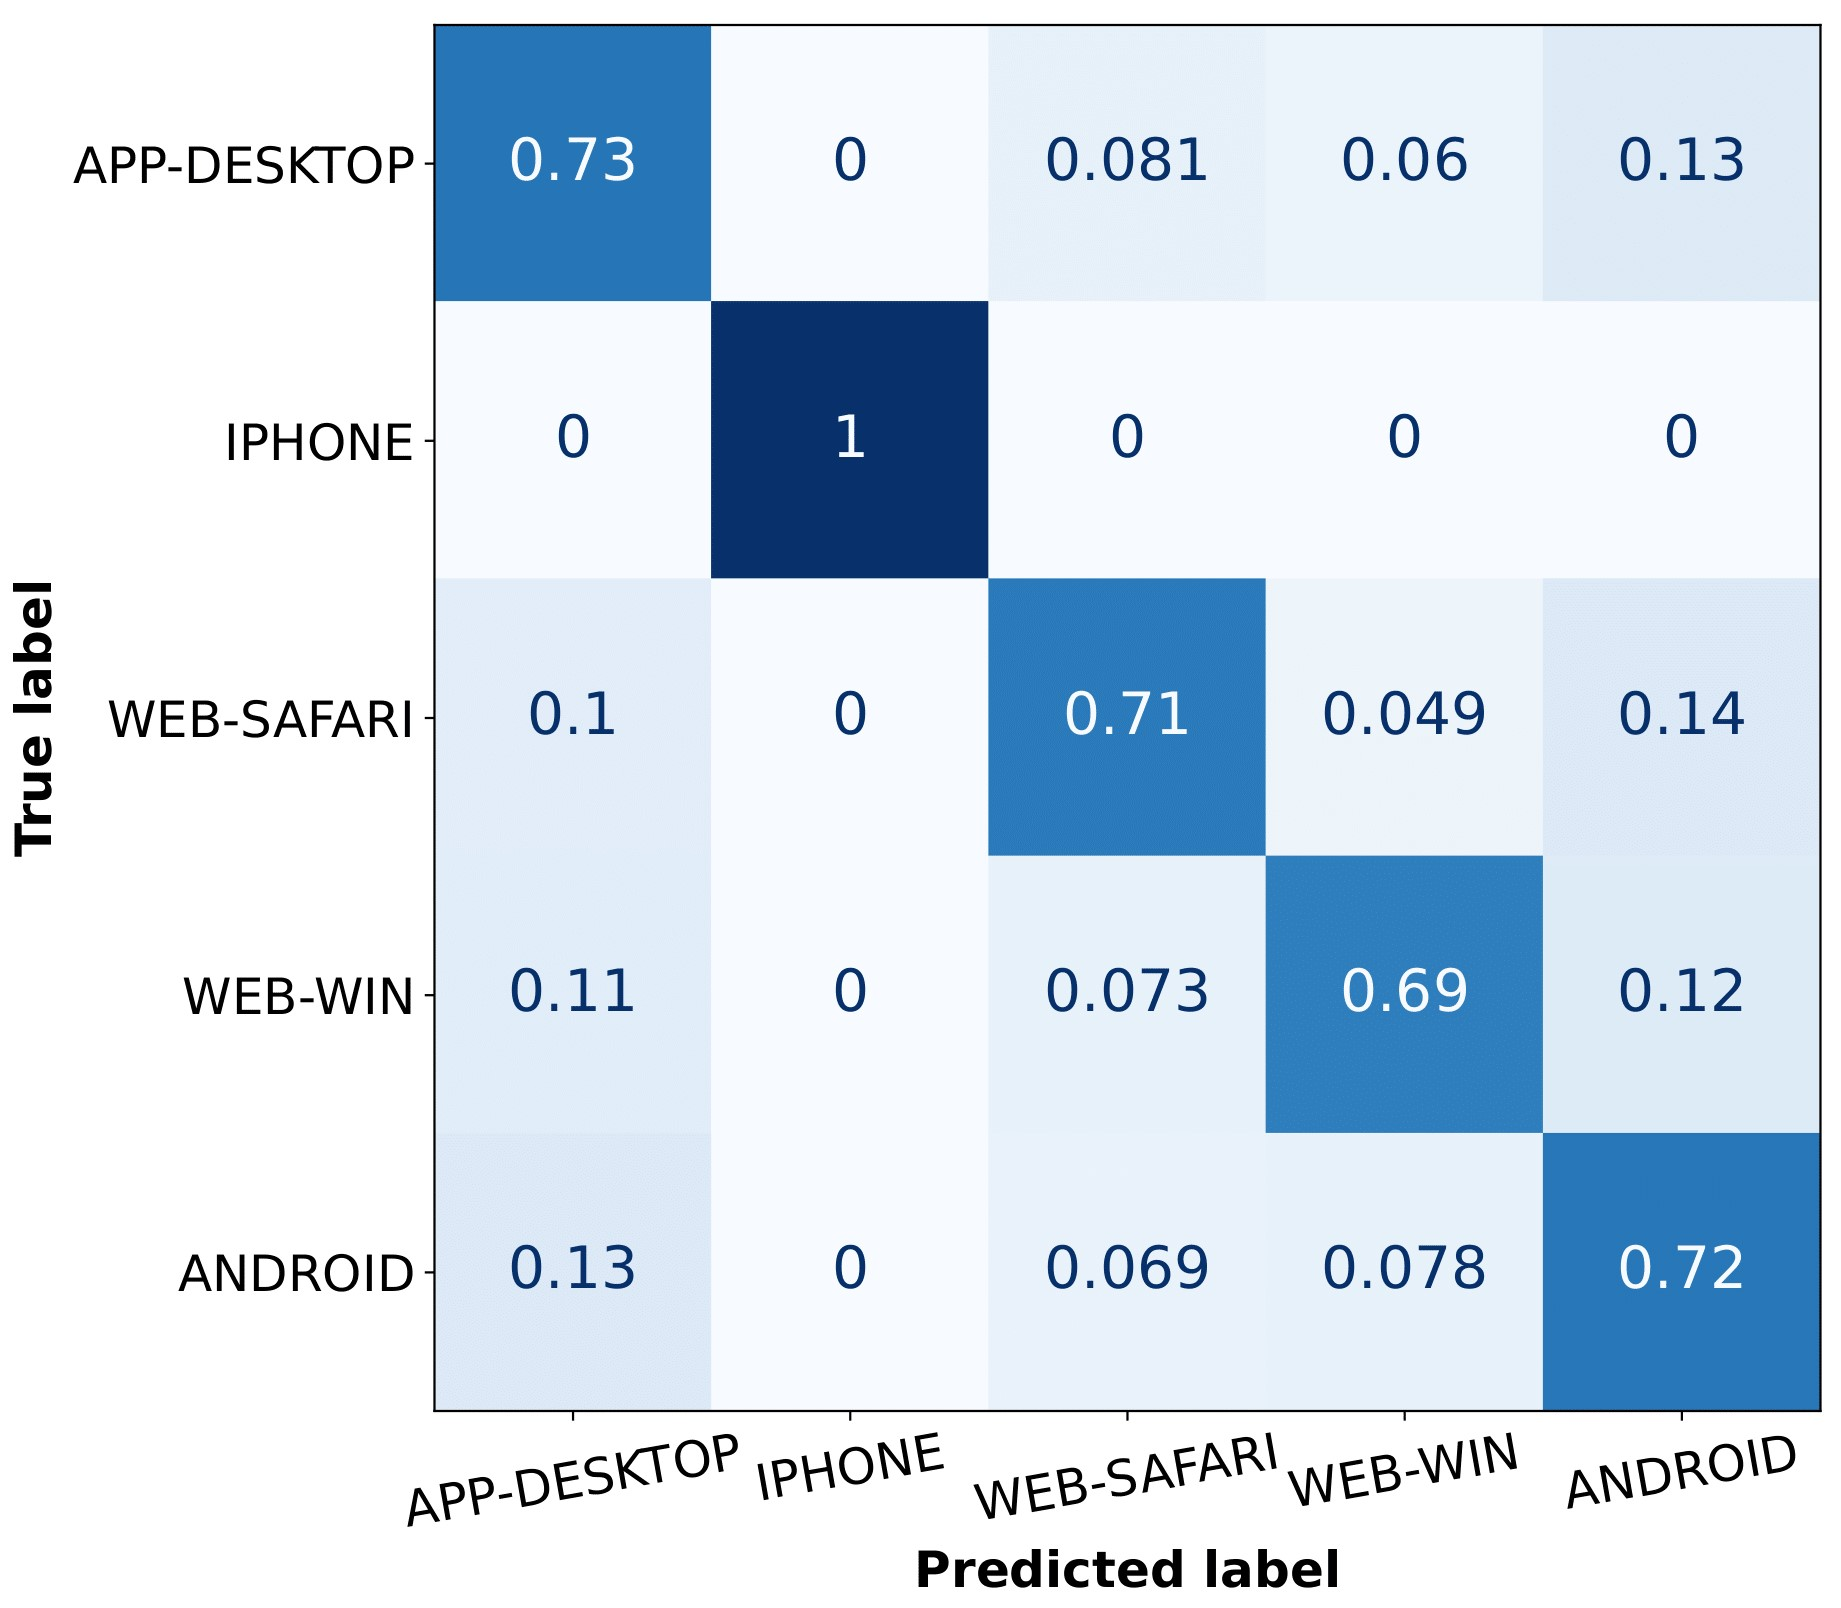
\includegraphics[width=8cm, height=8cm, keepaspectratio]{Immagini/Classificazione/confusion_matrix_RF.jpg}}\ \ \ \ \
    \subfloat[][]{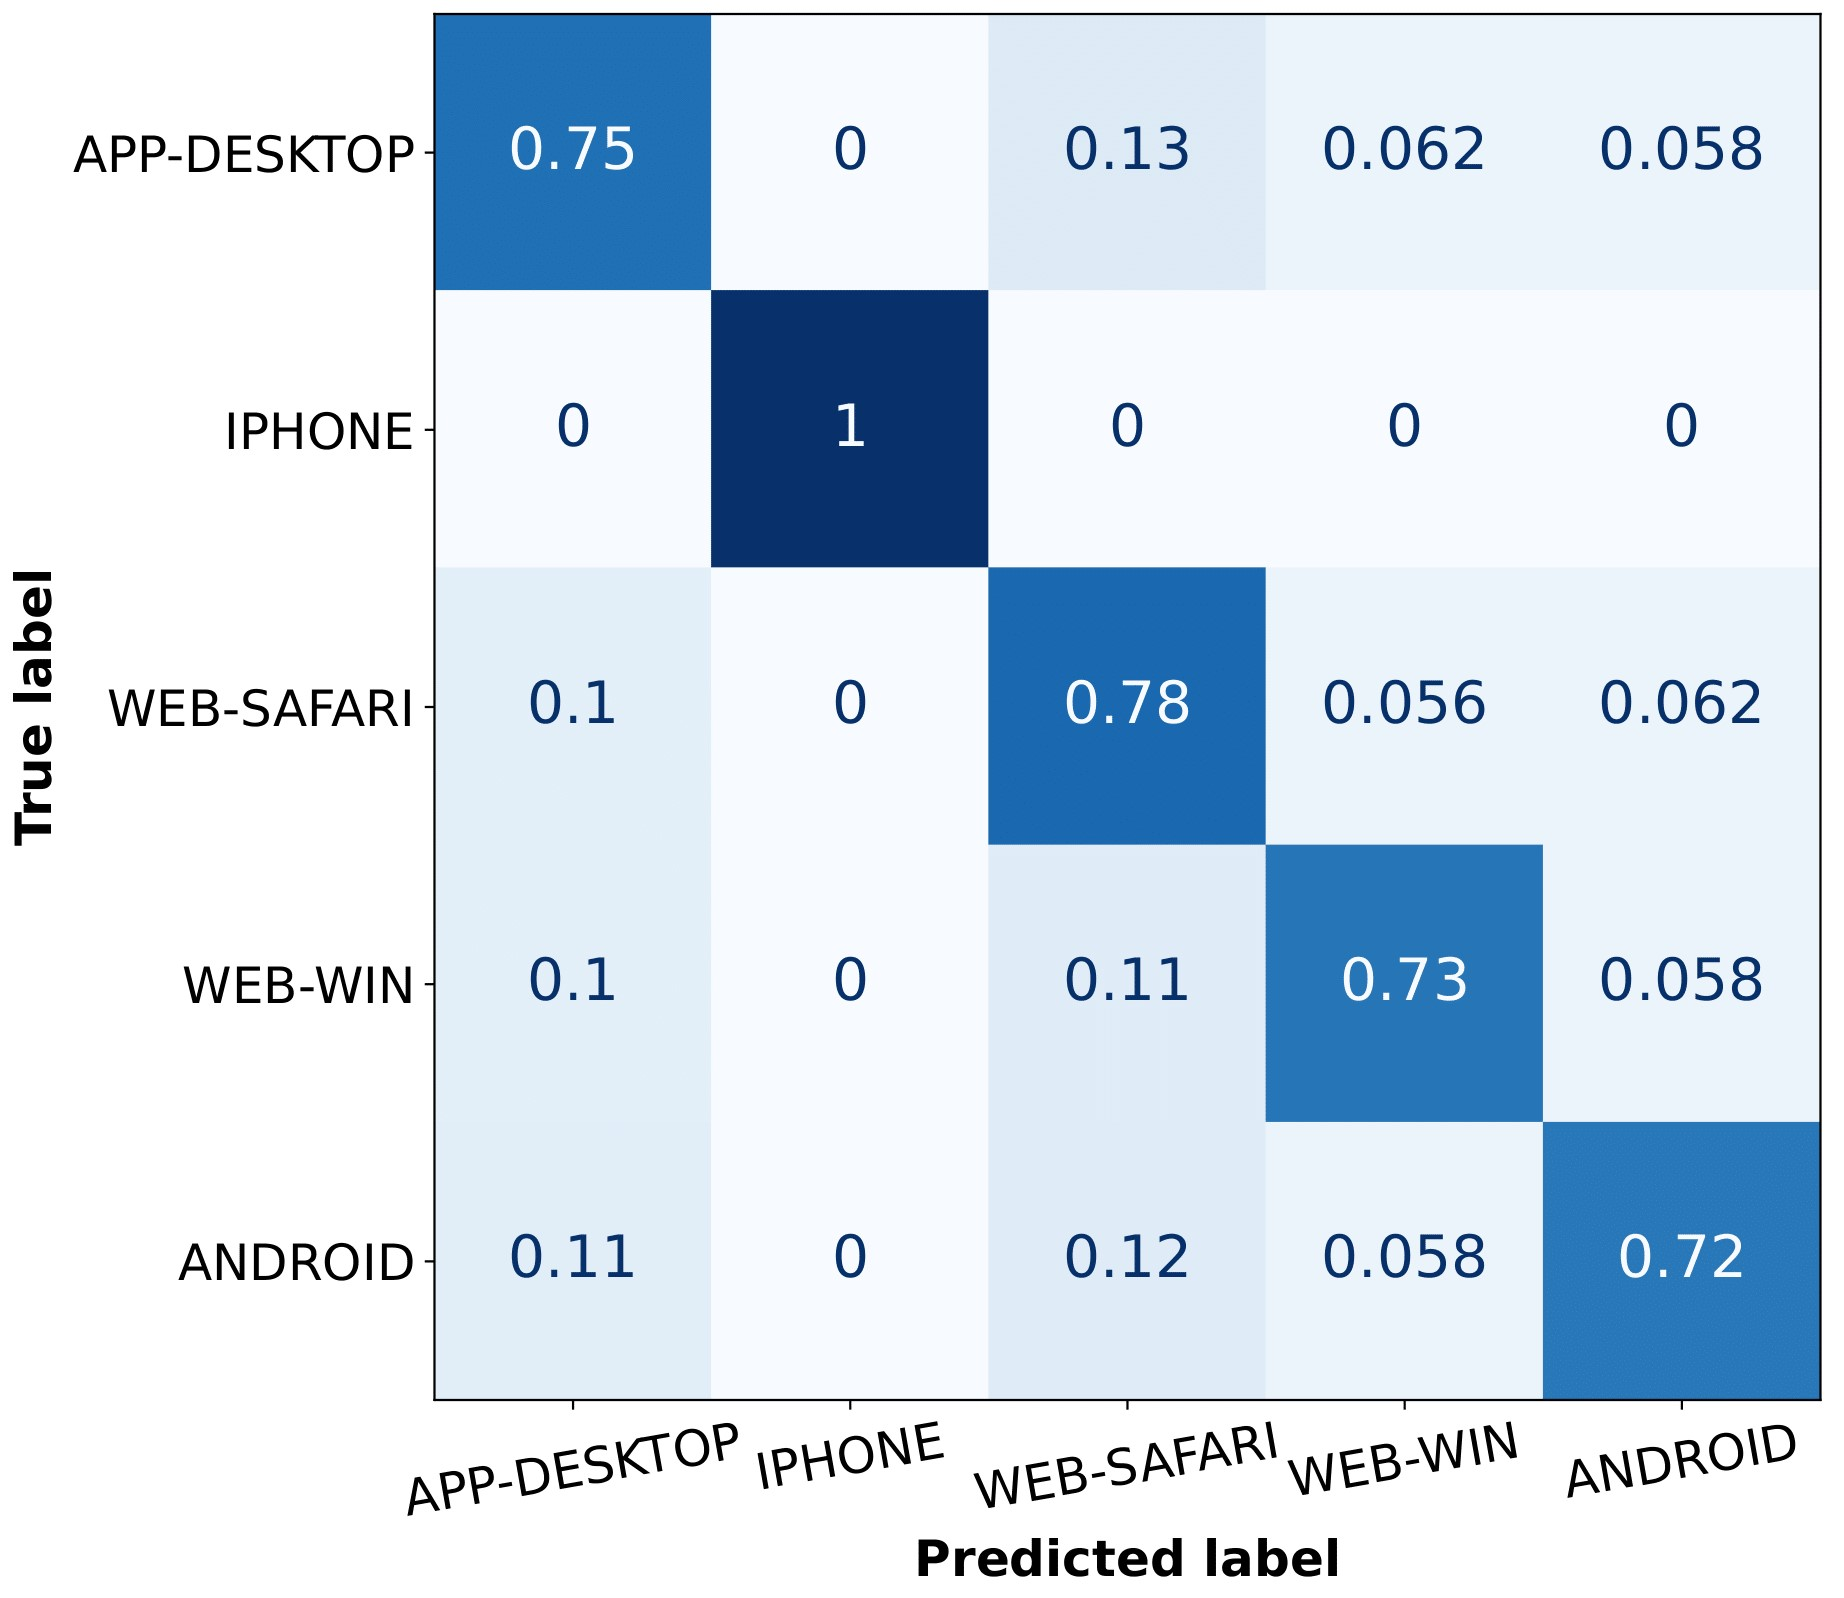
\includegraphics[width=8cm, height=8cm, keepaspectratio]{Immagini/Classificazione/confusion_matrix_SVM.jpg}}\\  
    \captionof{figure}{\textit{Confusion matrix} per la classificazione delle immagini di SHADE con (a) \textit{random forest} e (b) \textit{support vector machine}.}
    \label{fig:class}
\endgroup

\vspace{1em}

\begingroup
    \centering
    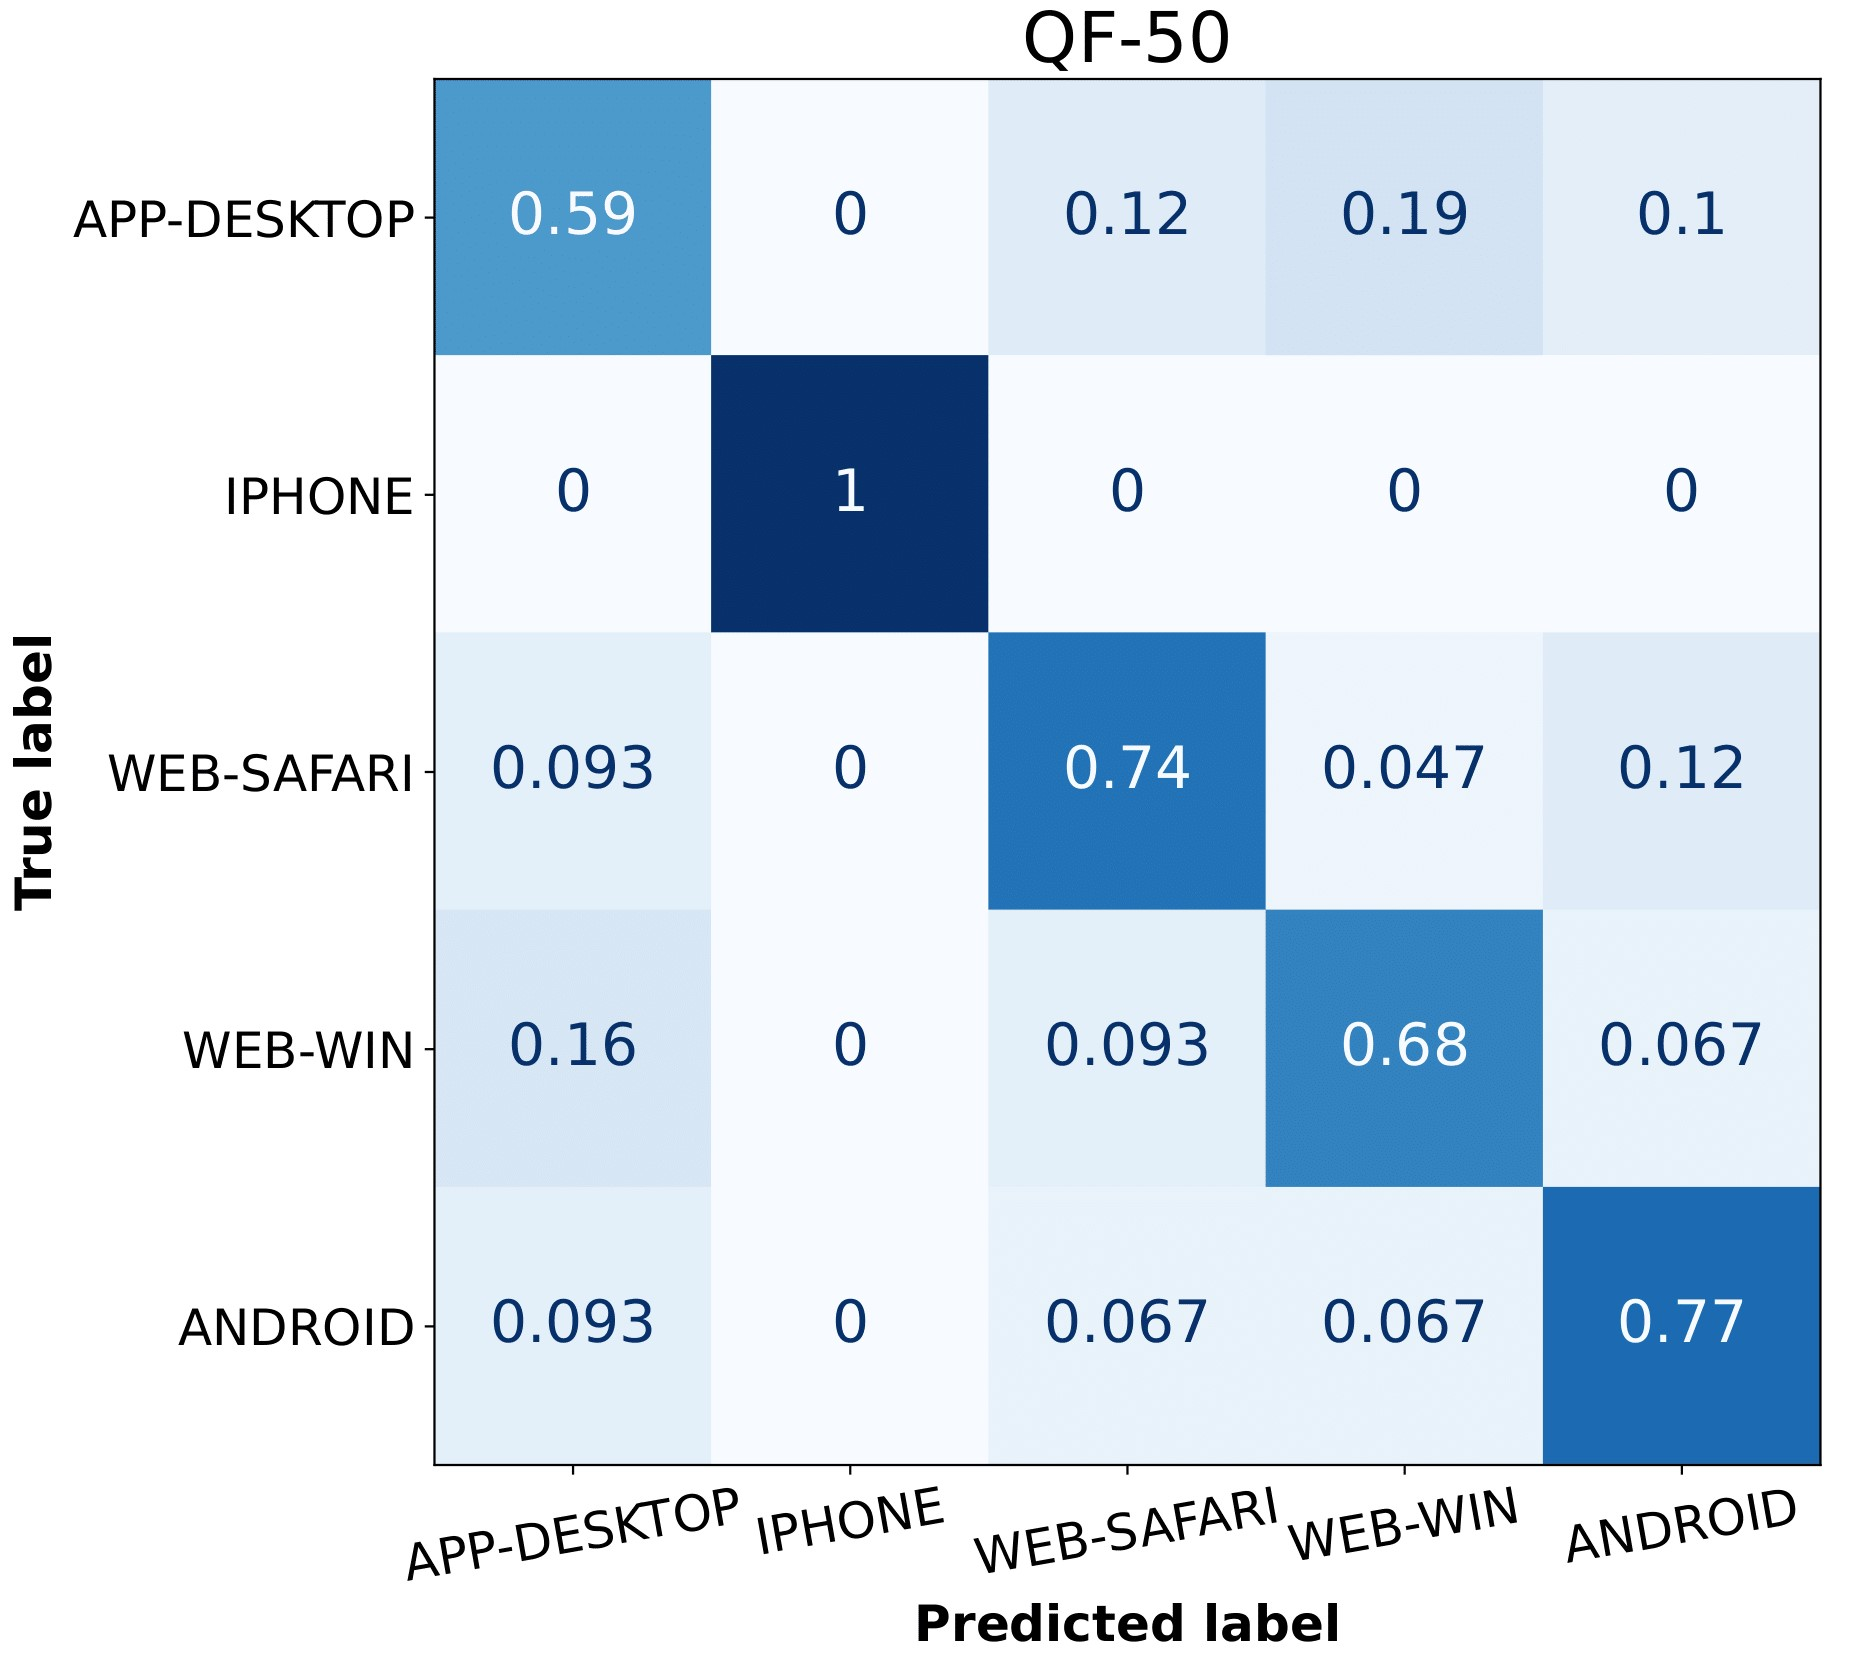
\includegraphics[width=8cm, height=8cm, keepaspectratio]{Immagini/Classificazione/confusion_matrix_RF_QF-50.jpg}\ \ \ \ \
    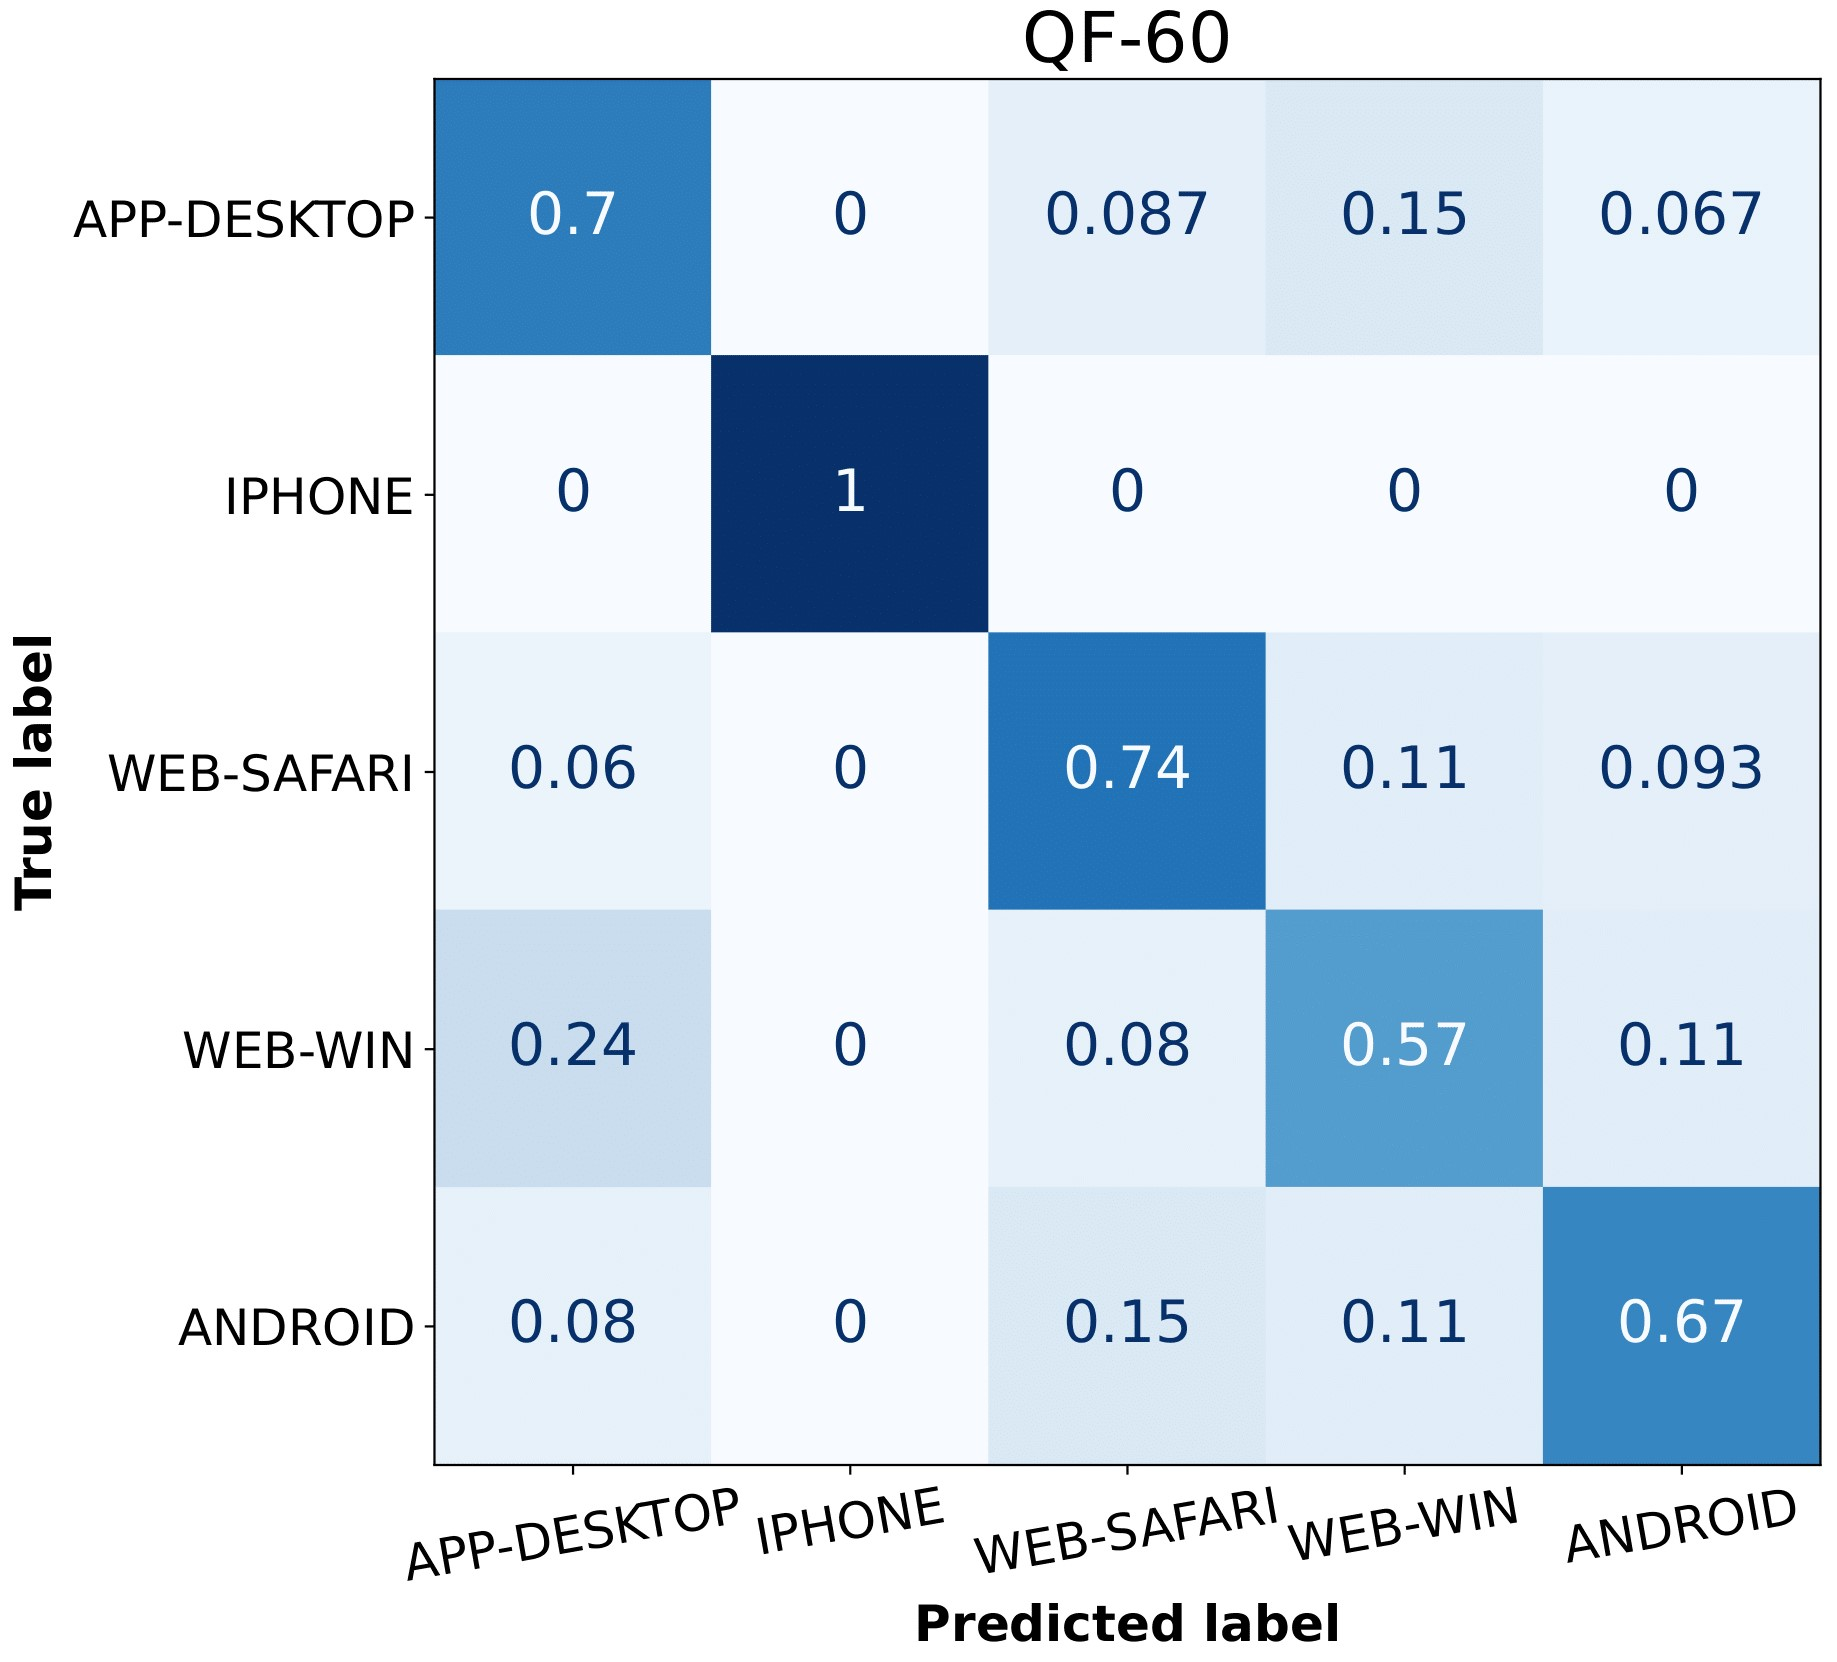
\includegraphics[width=8cm, height=8cm, keepaspectratio]{Immagini/Classificazione/confusion_matrix_RF_QF-60.jpg}\\\vspace{1em}
    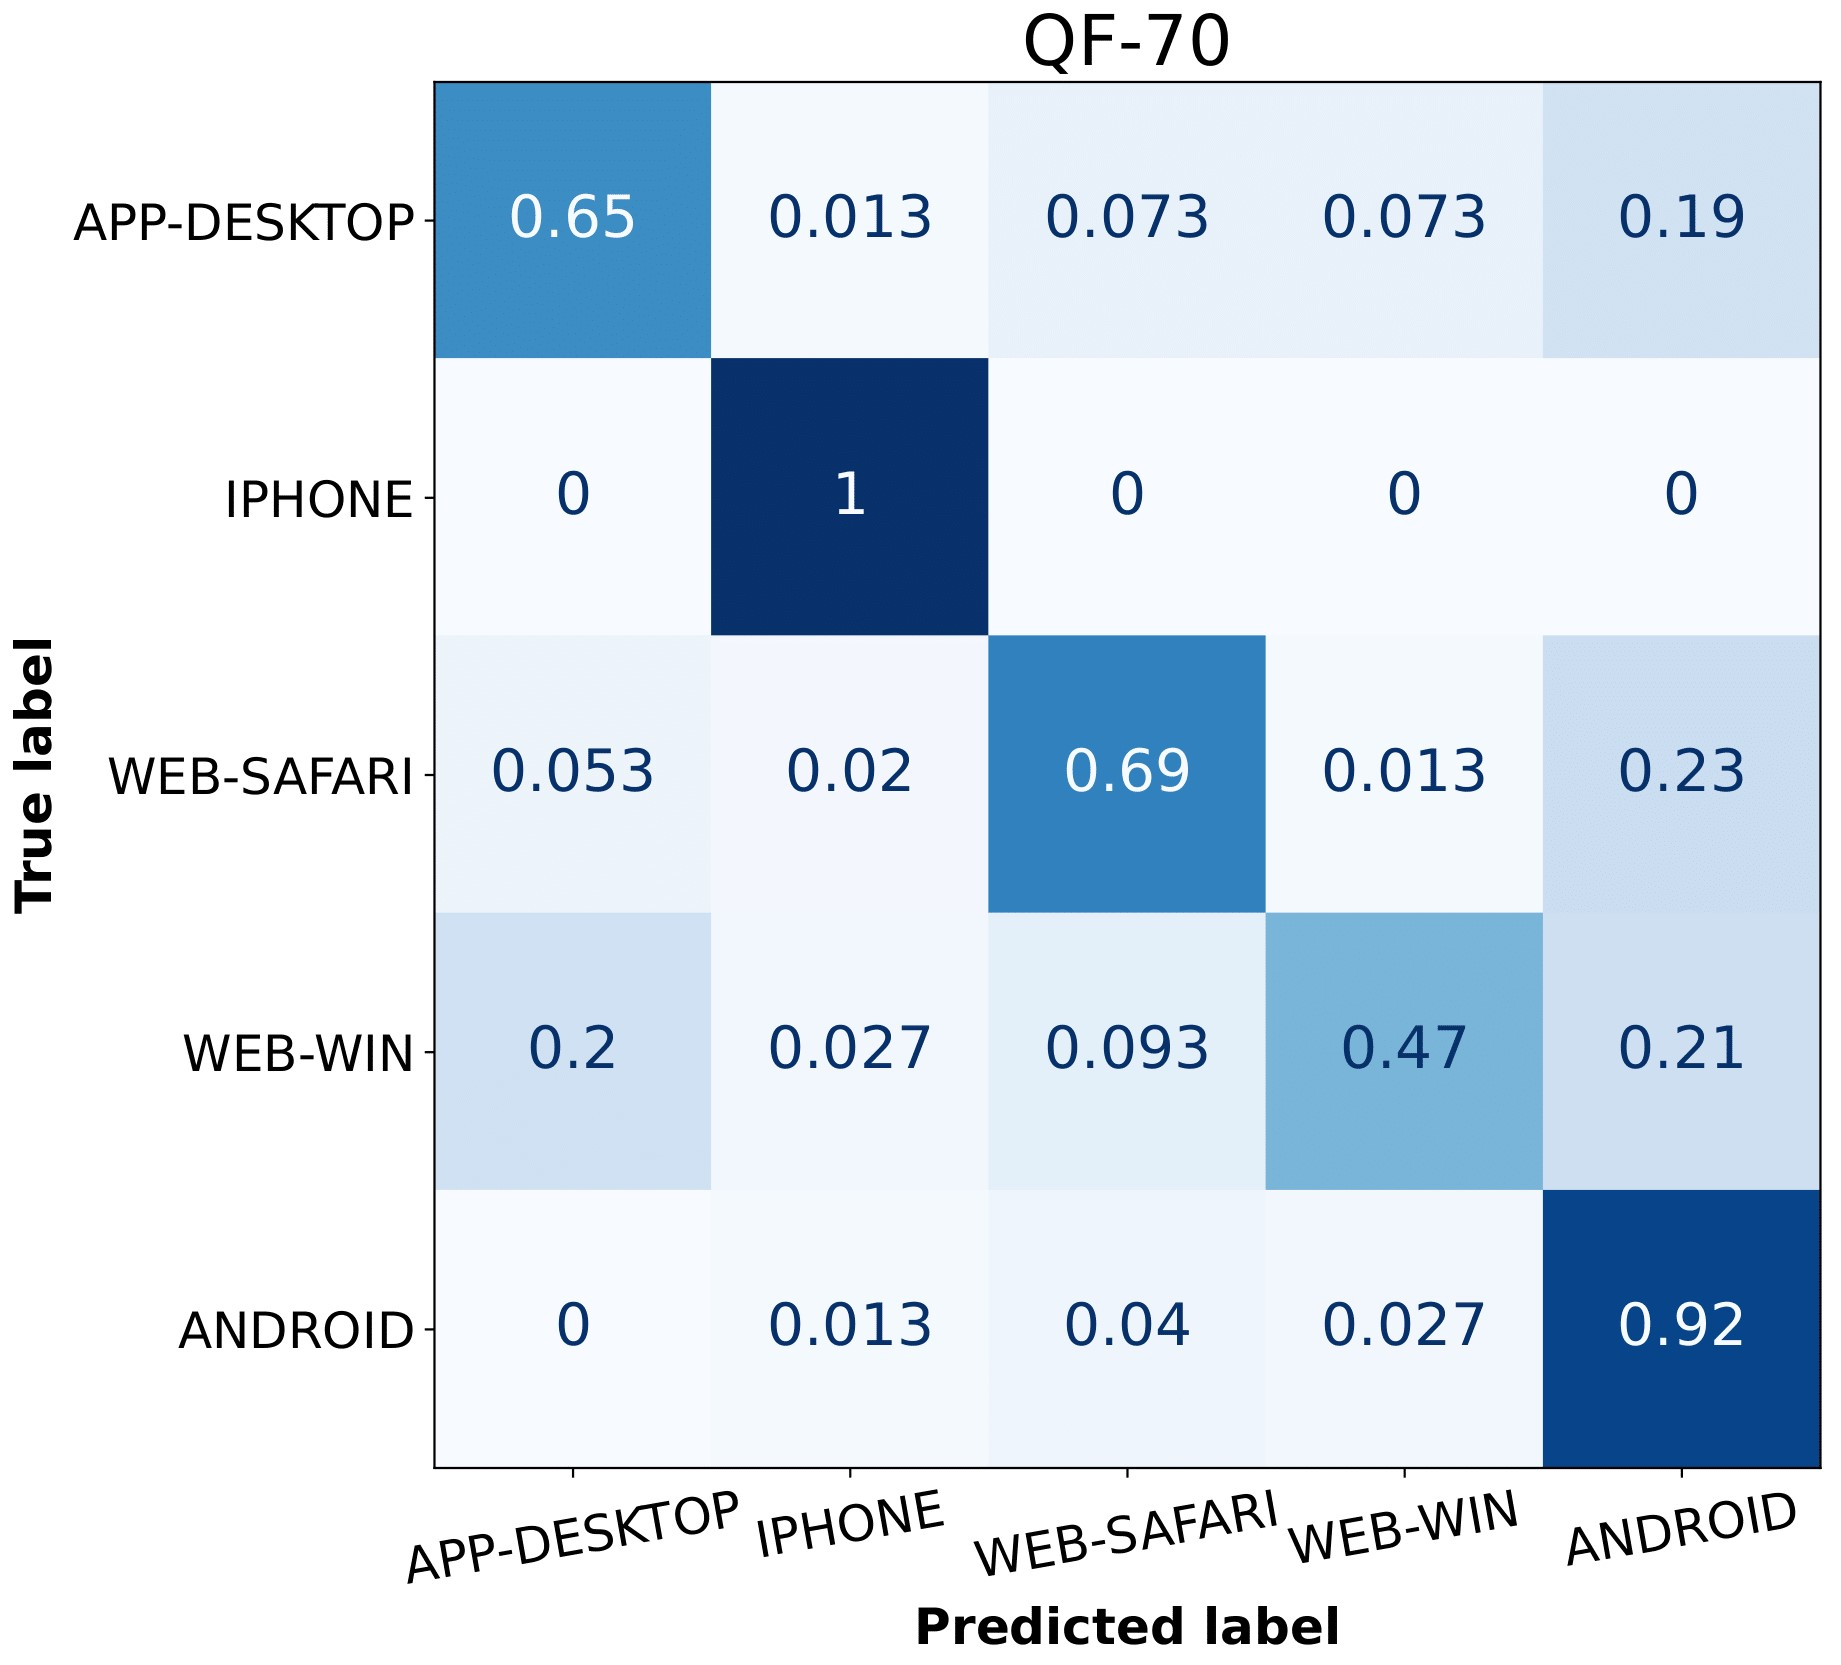
\includegraphics[width=8cm, height=8cm, keepaspectratio]{Immagini/Classificazione/confusion_matrix_RF_QF-70.jpg}\ \ \ \ \
    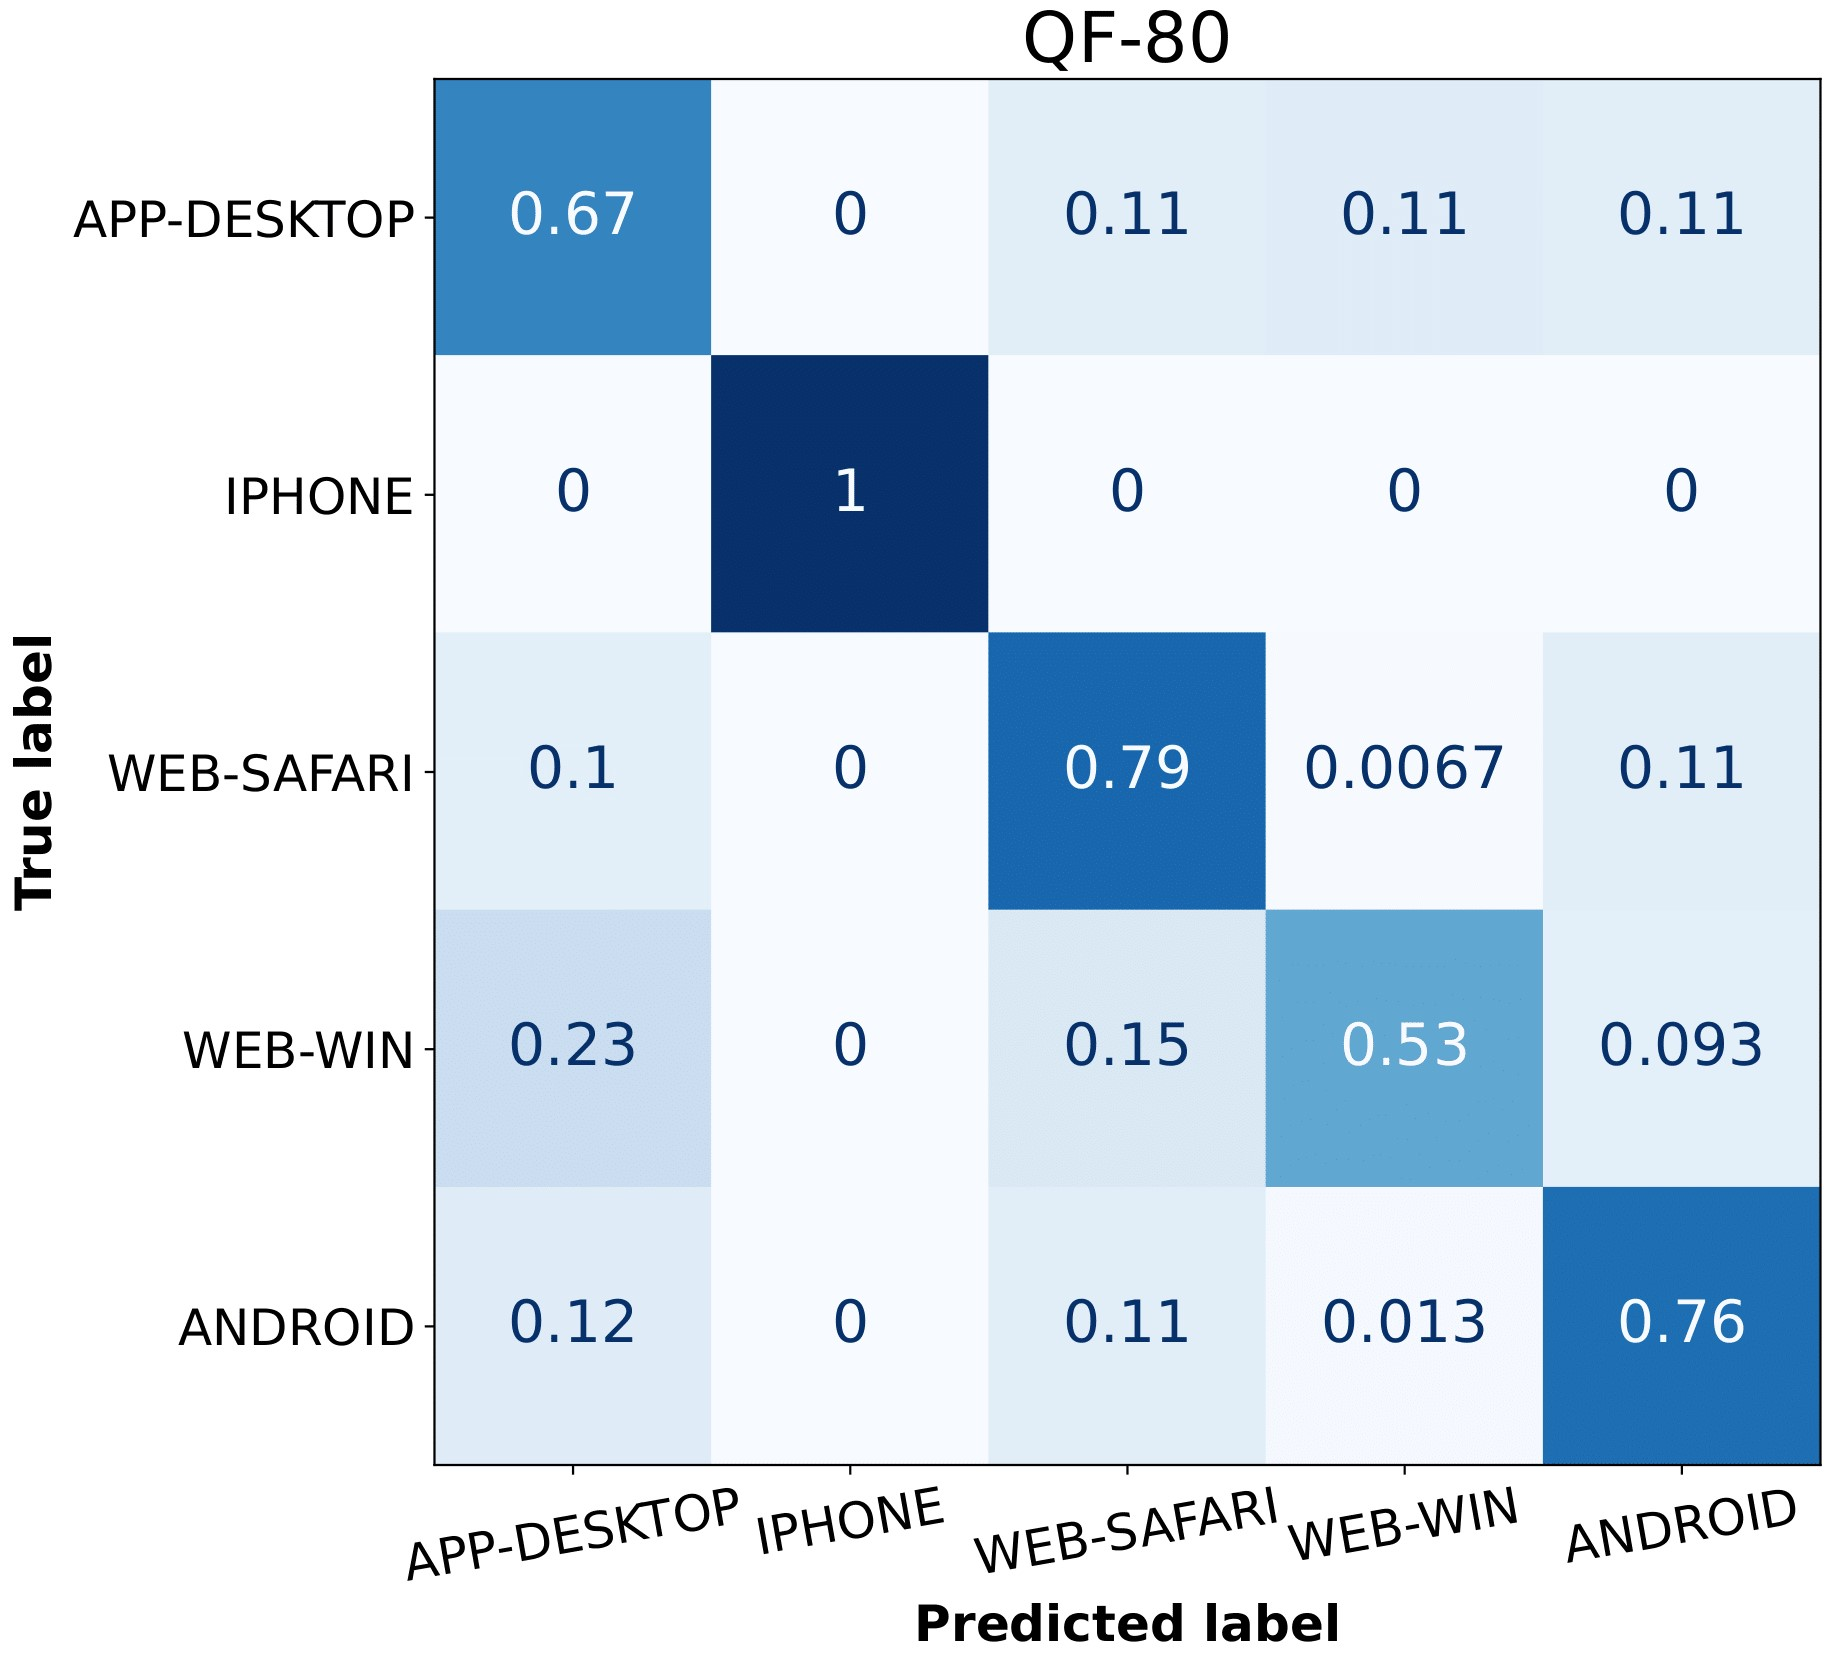
\includegraphics[width=8cm, height=8cm, keepaspectratio]{Immagini/Classificazione/confusion_matrix_RF_QF-80.jpg}\\\vspace{1em}
    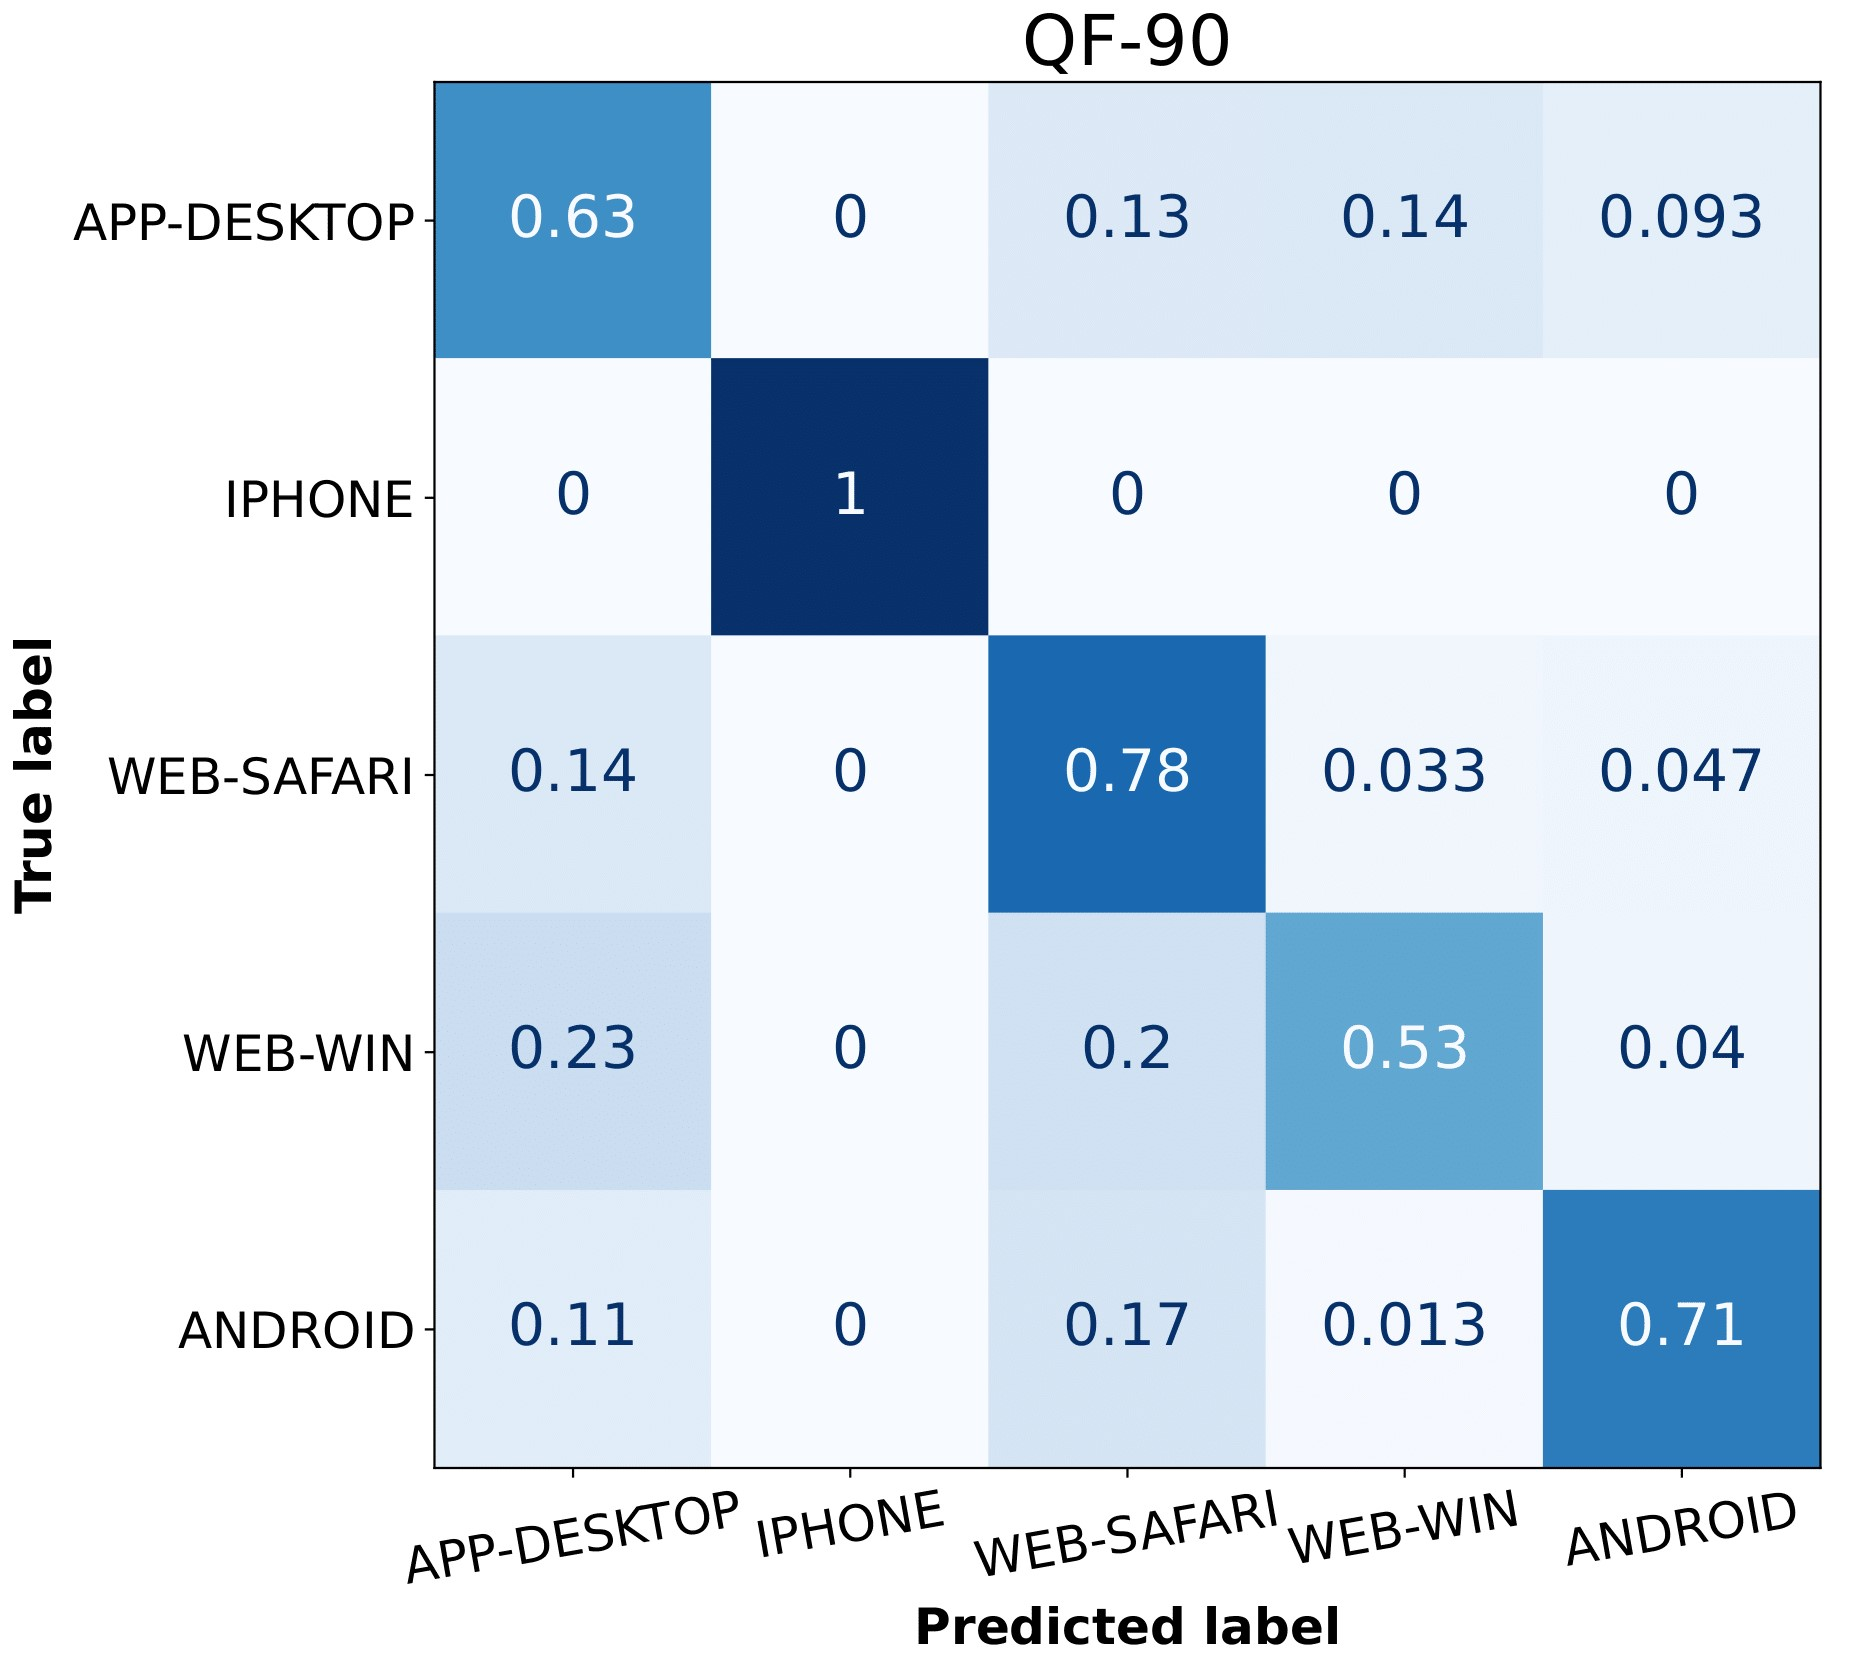
\includegraphics[width=8cm, height=8cm, keepaspectratio]{Immagini/Classificazione/confusion_matrix_RF_QF-90.jpg}\ \ \ \ \
    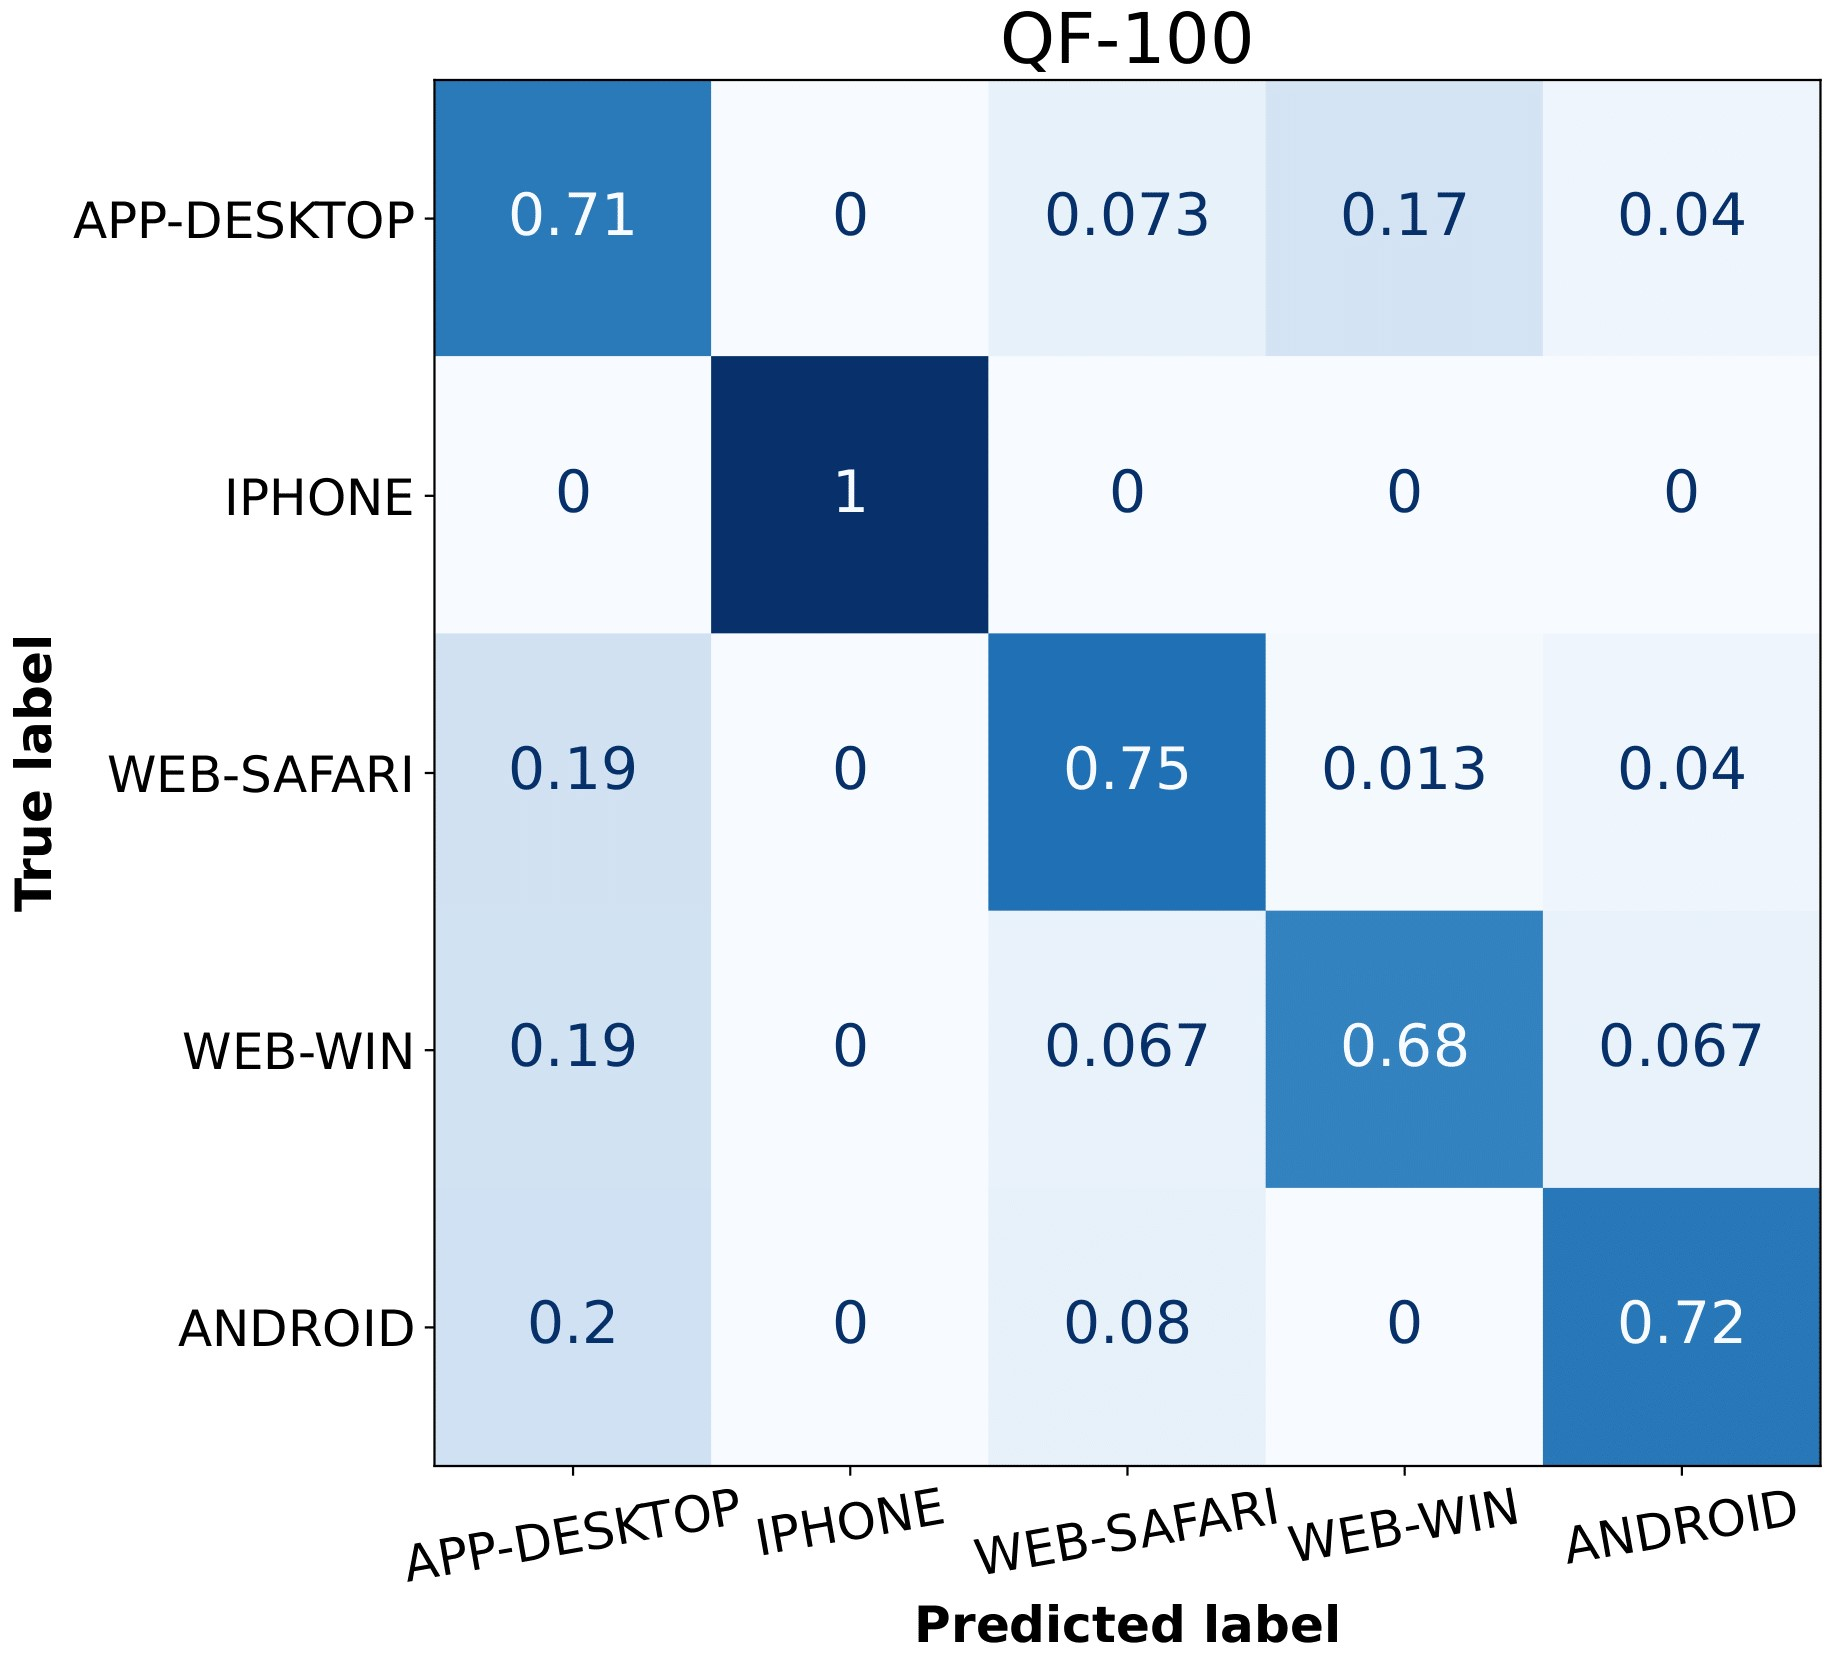
\includegraphics[width=8cm, height=8cm, keepaspectratio]{Immagini/Classificazione/confusion_matrix_RF_QF-100.jpg}
    \captionof{figure}{\textit{Confusion matrix} per \textit{random forest} divise per \textit{quality factor}.}
    \label{fig:class_QF_RF}
\endgroup

\vspace{3em}

\begingroup
    \centering
    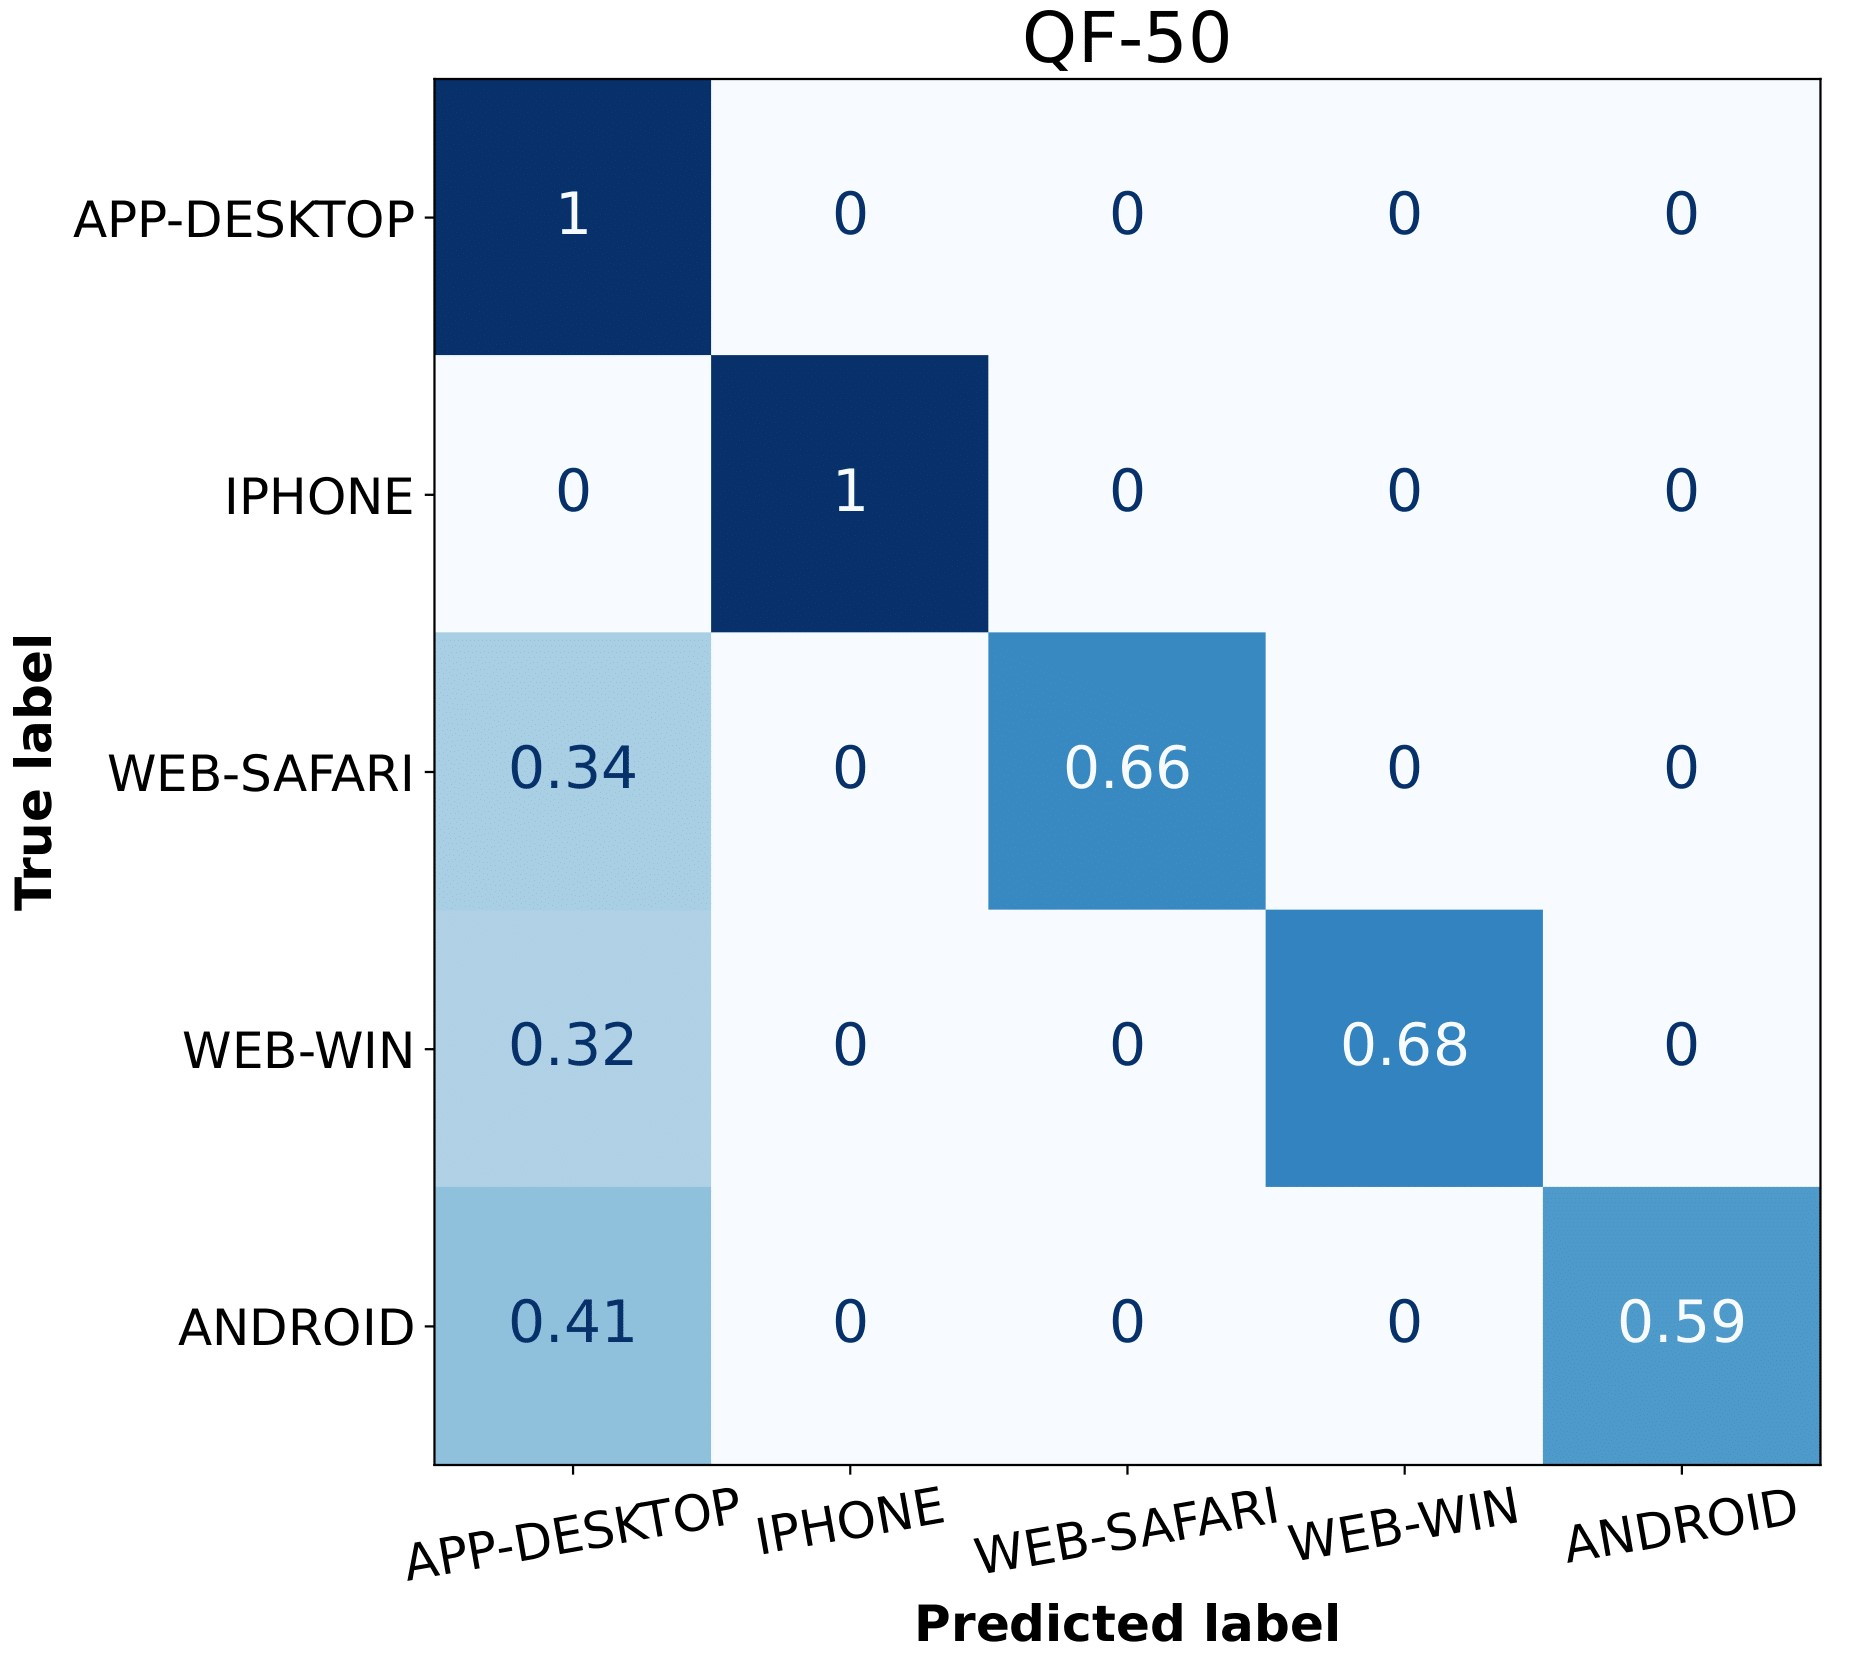
\includegraphics[width=8cm, height=8cm, keepaspectratio]{Immagini/Classificazione/confusion_matrix_SVM_QF-50.jpg}\ \ \ \ \
    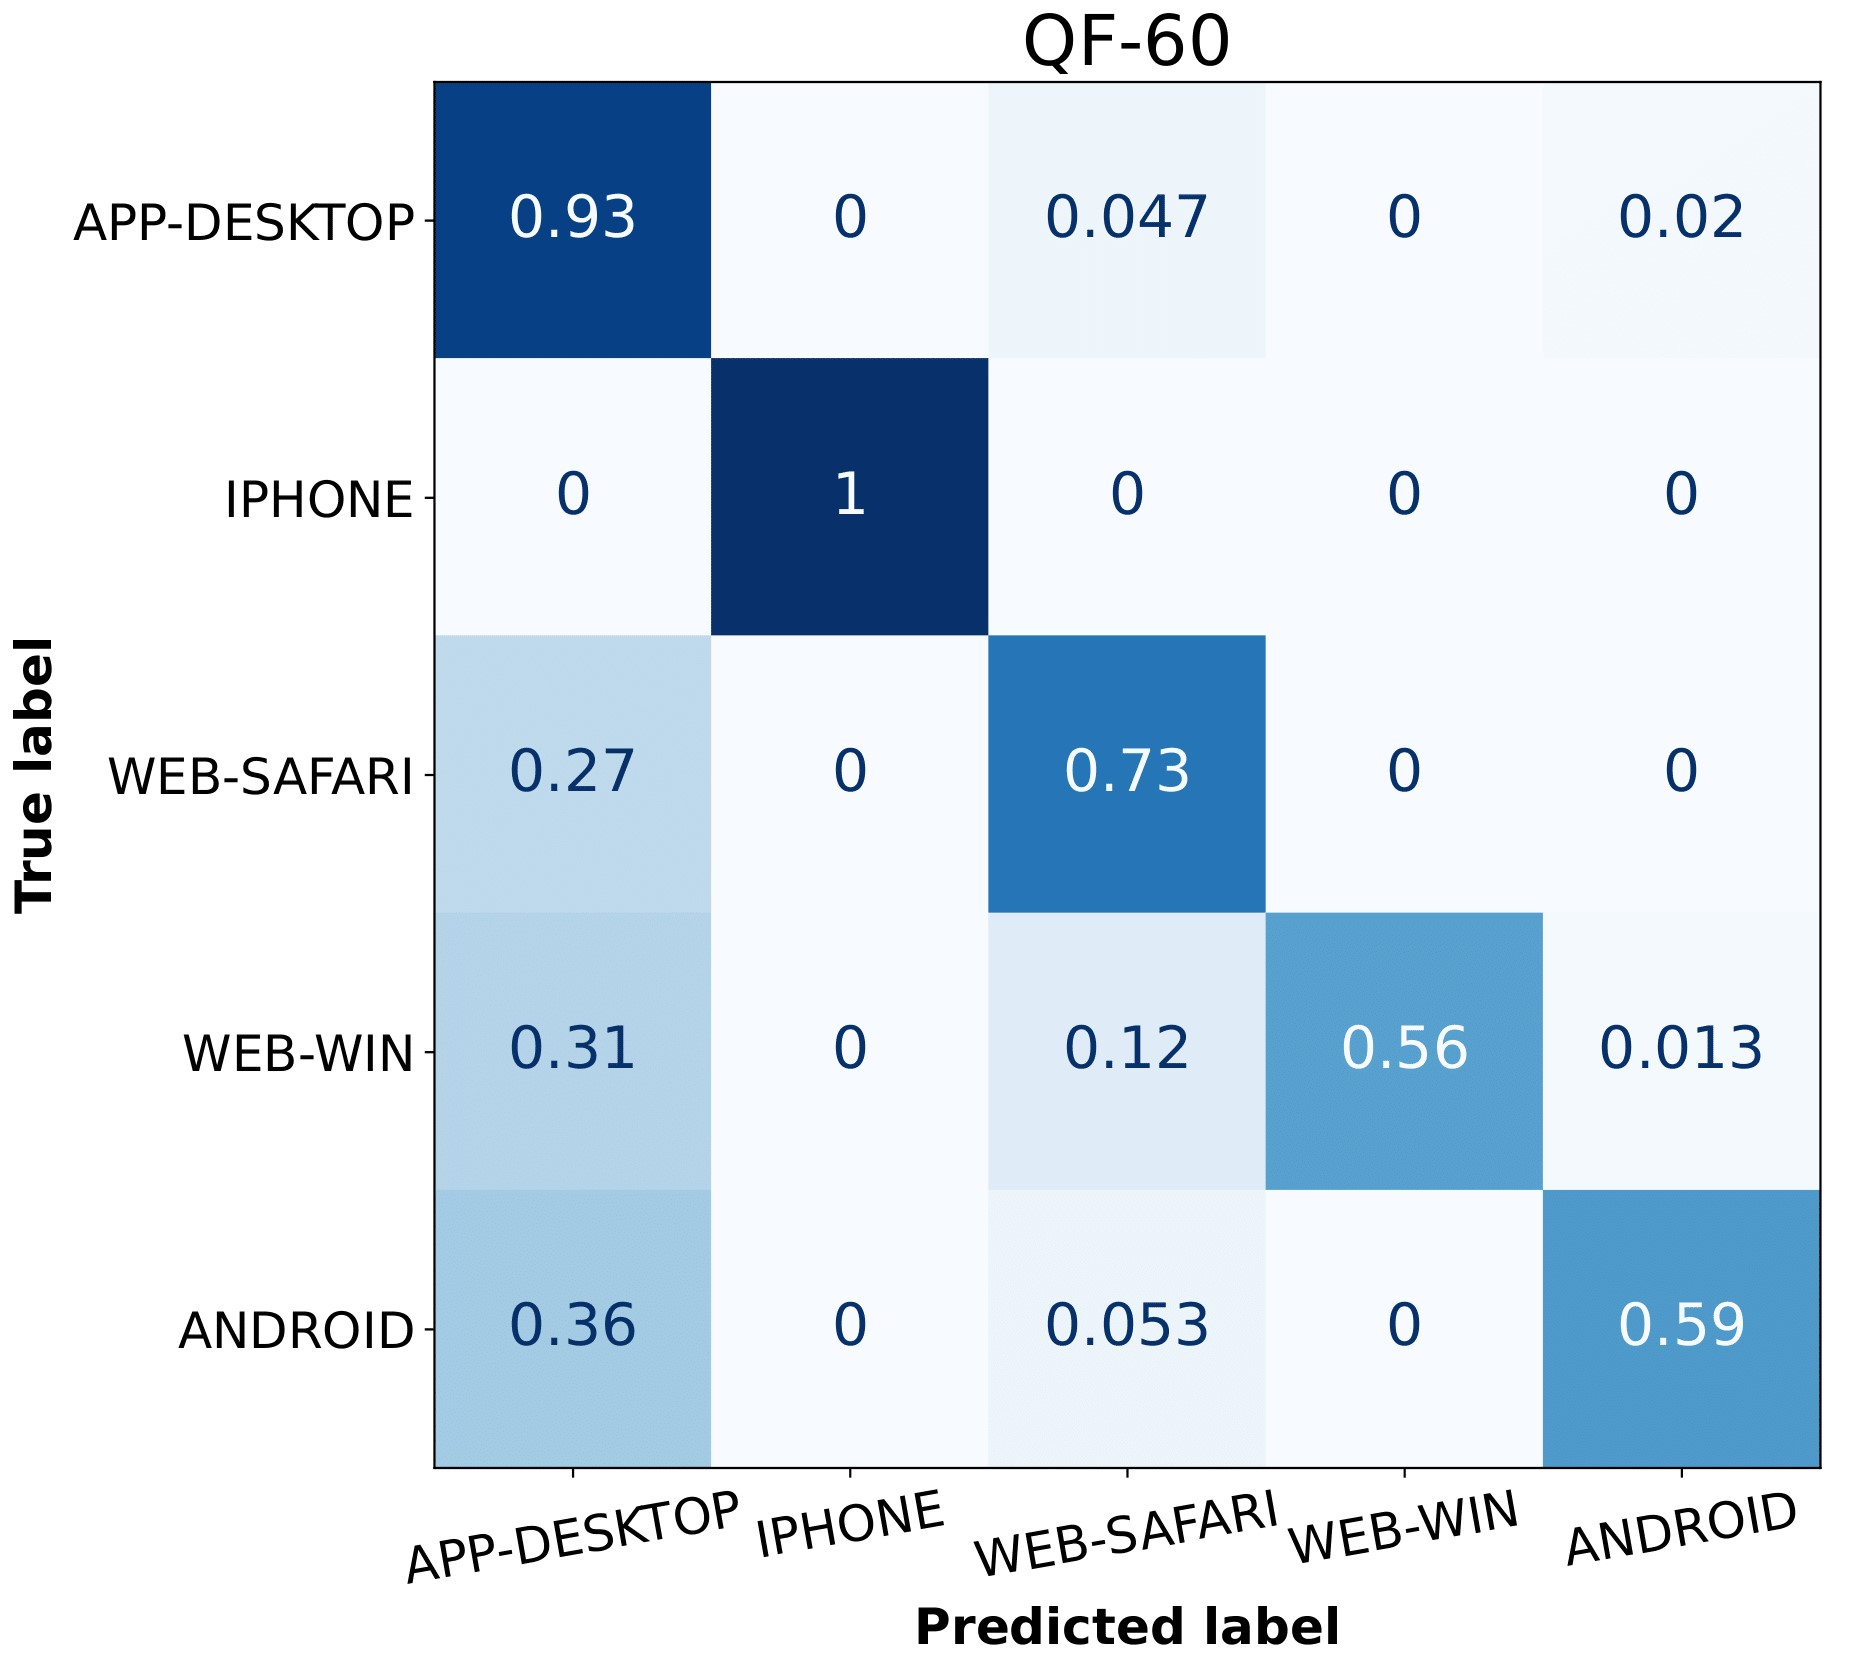
\includegraphics[width=8cm, height=8cm, keepaspectratio]{Immagini/Classificazione/confusion_matrix_SVM_QF-60.jpg}\\\vspace{1em}
    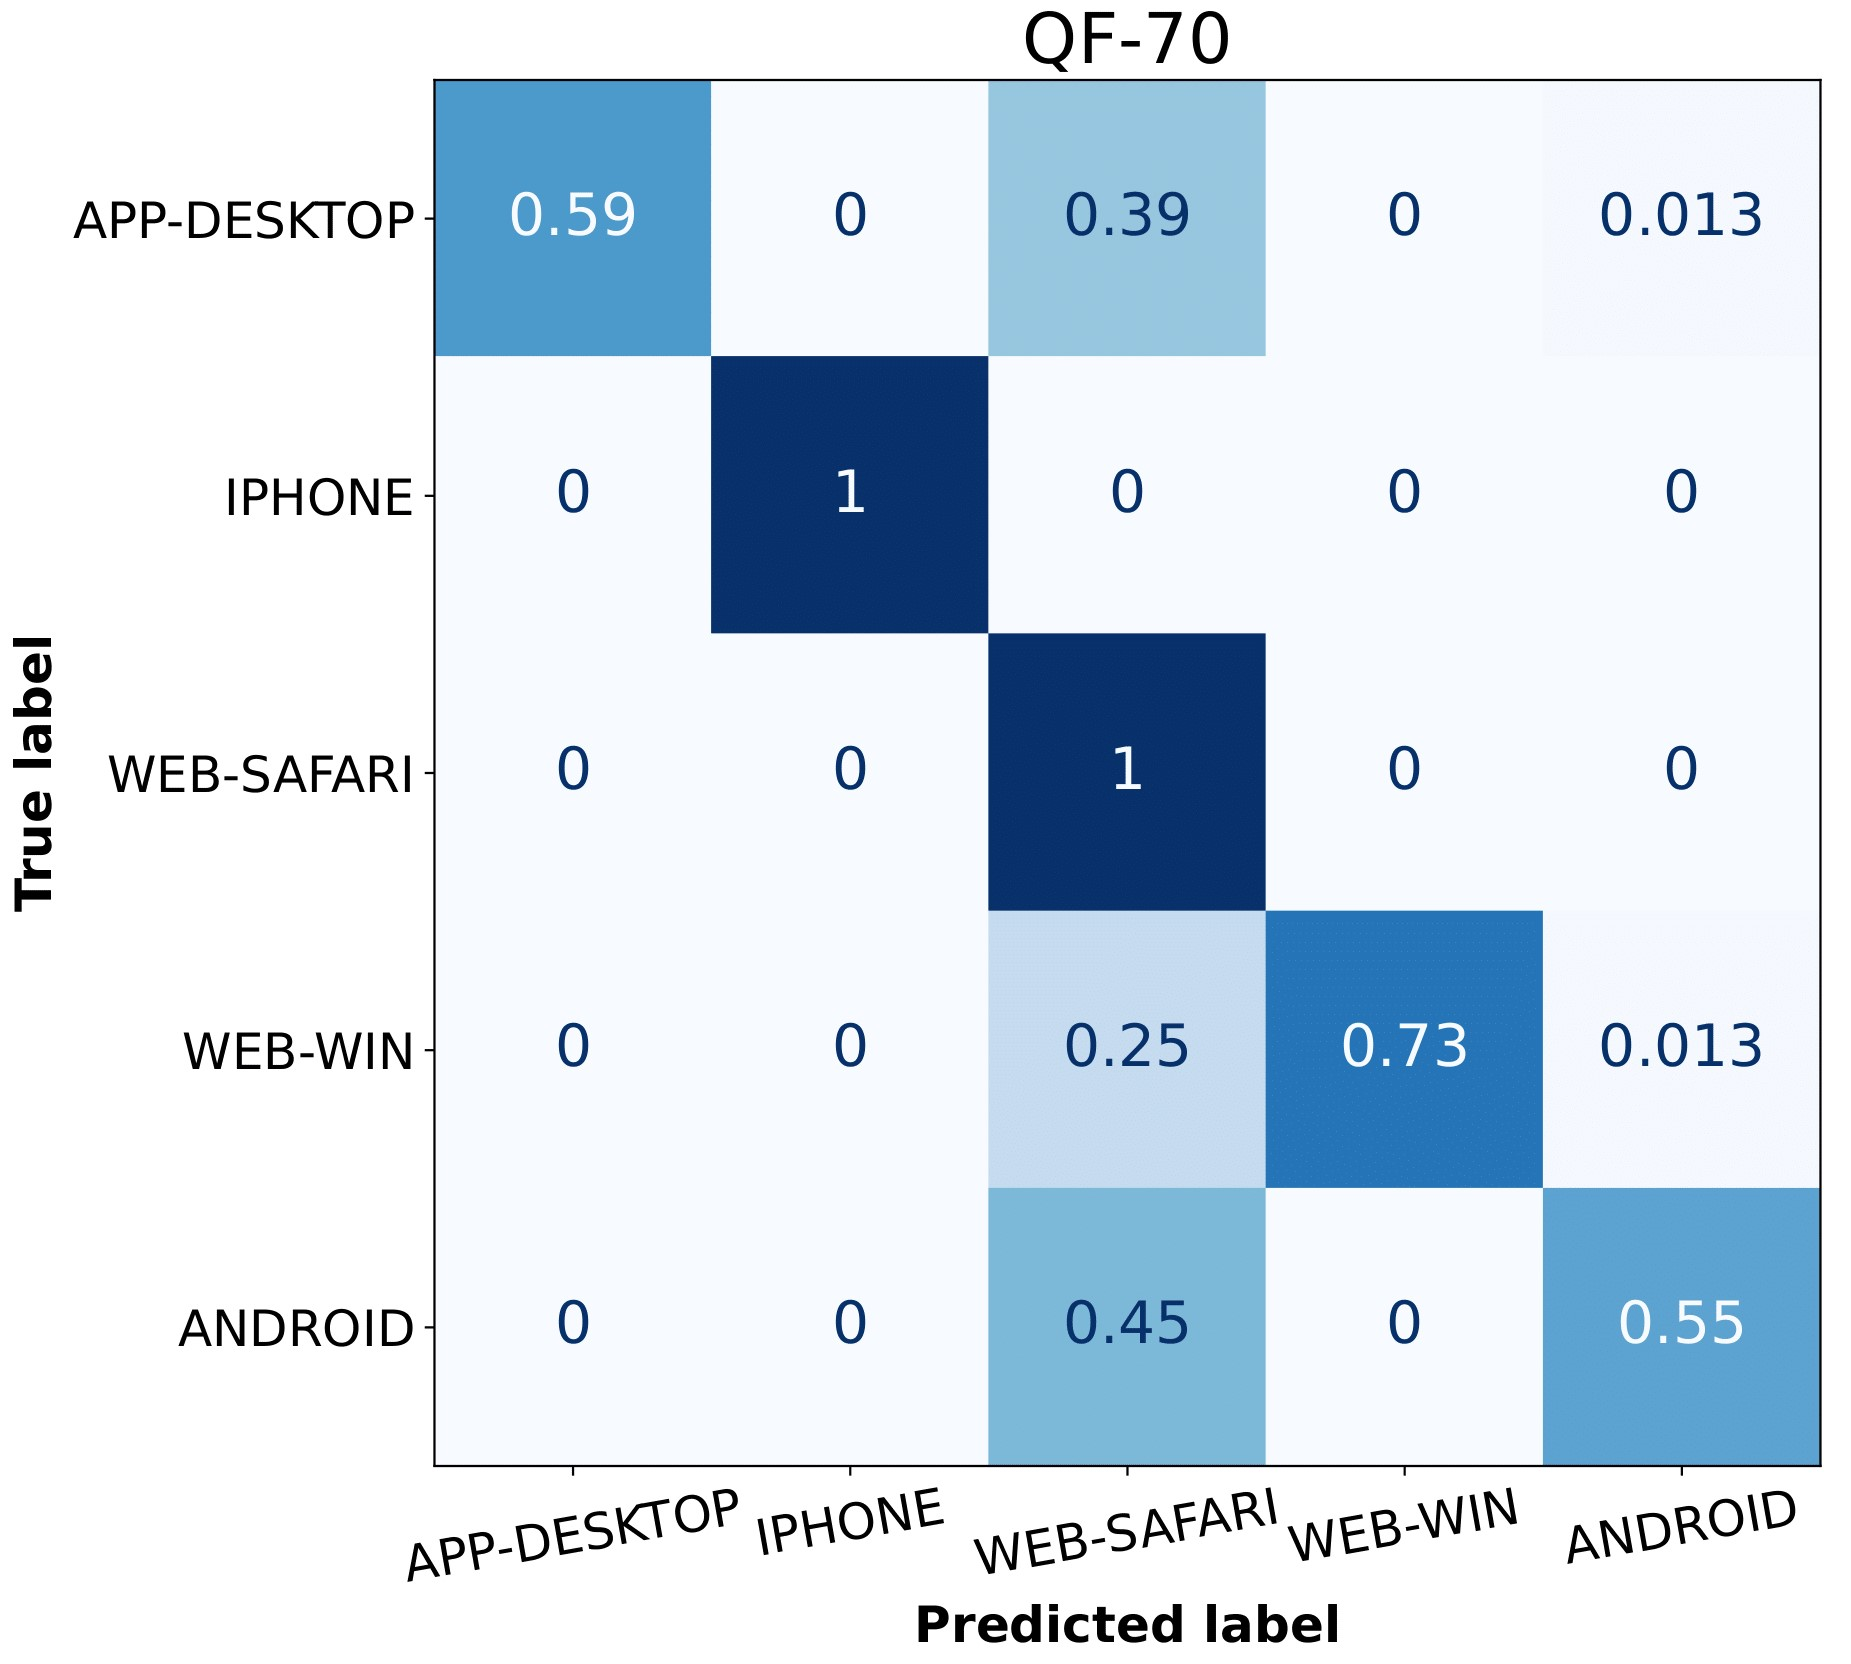
\includegraphics[width=8cm, height=8cm, keepaspectratio]{Immagini/Classificazione/confusion_matrix_SVM_QF-70.jpg}\ \ \ \ \
    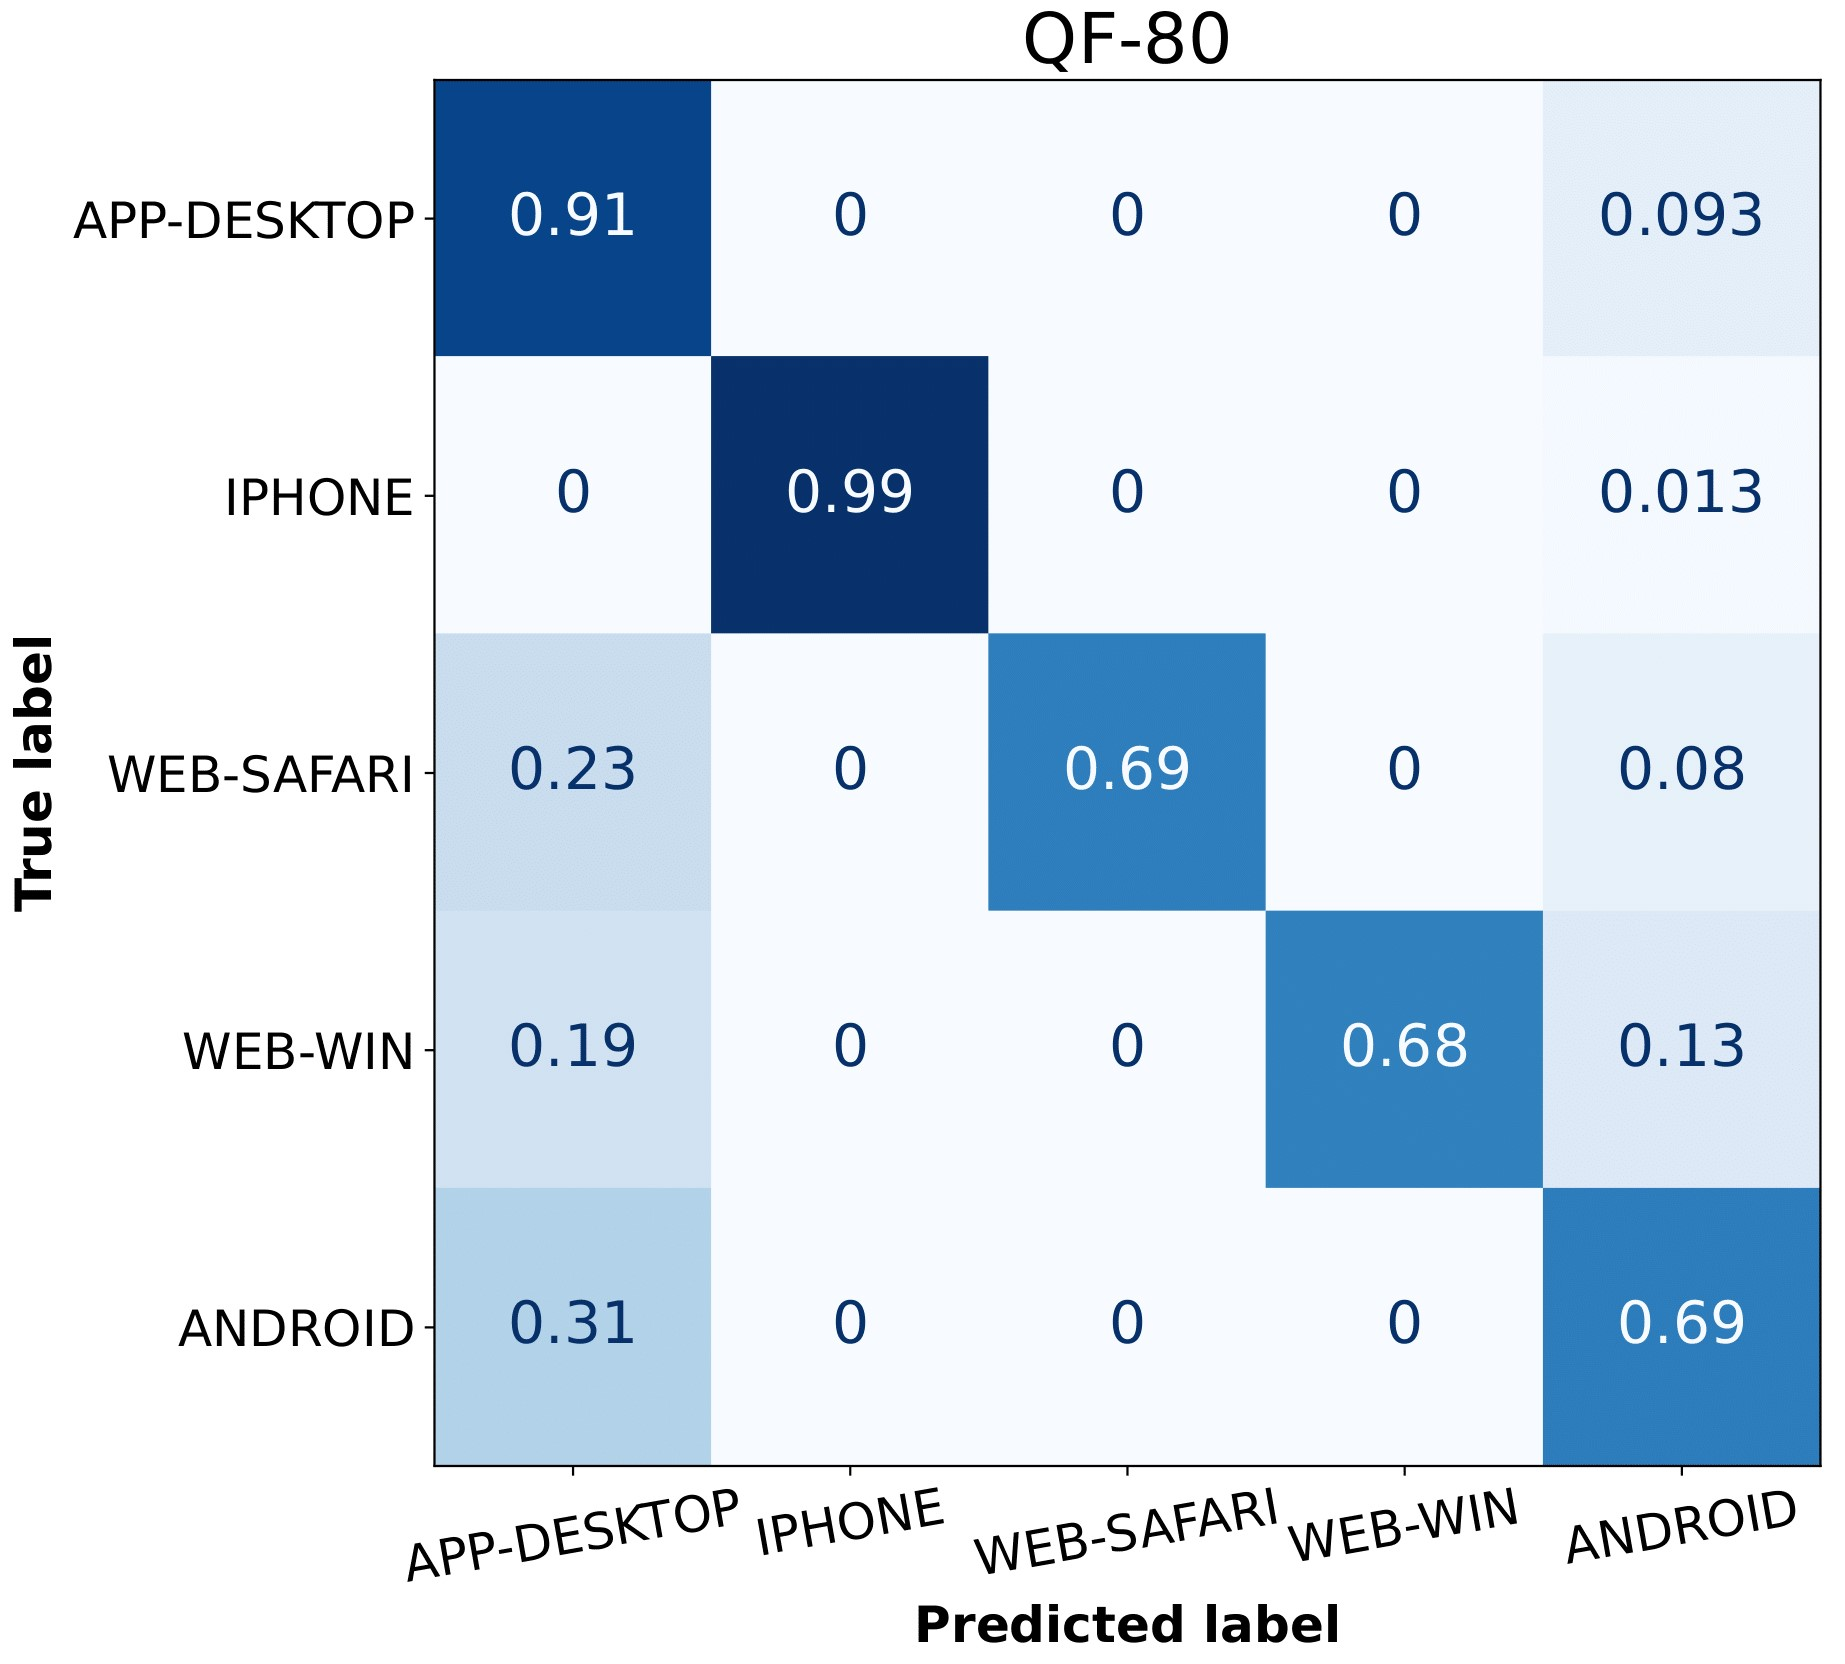
\includegraphics[width=8cm, height=8cm, keepaspectratio]{Immagini/Classificazione/confusion_matrix_SVM_QF-80.jpg}\\\vspace{1em}
    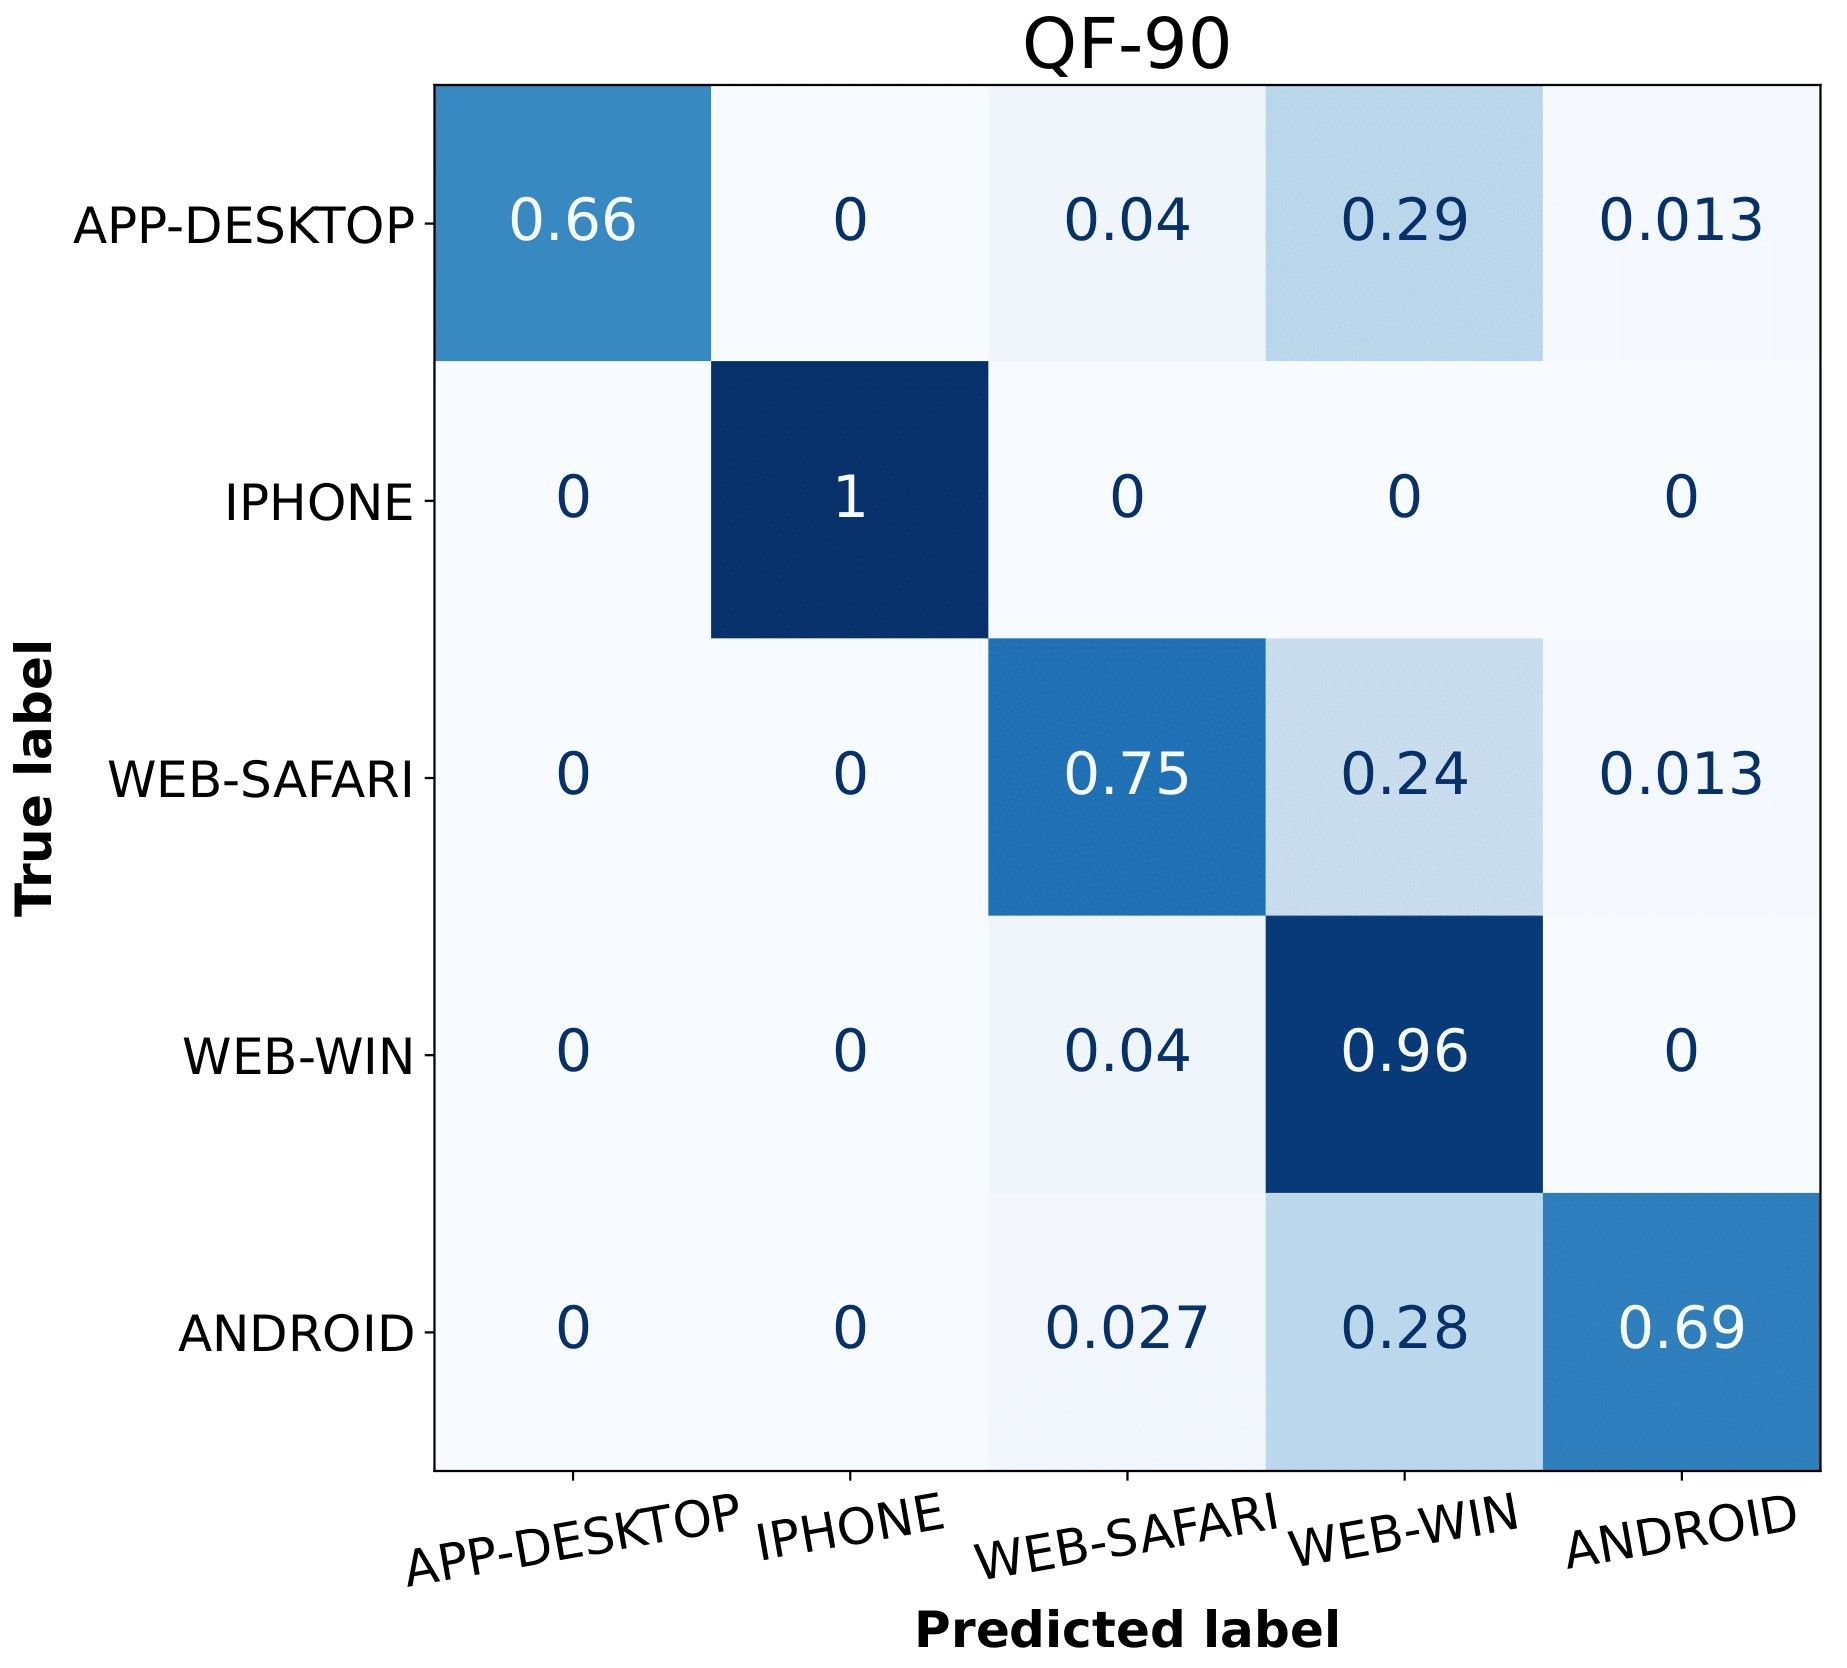
\includegraphics[width=8cm, height=8cm, keepaspectratio]{Immagini/Classificazione/confusion_matrix_SVM_QF-90.jpg}\ \ \ \ \
    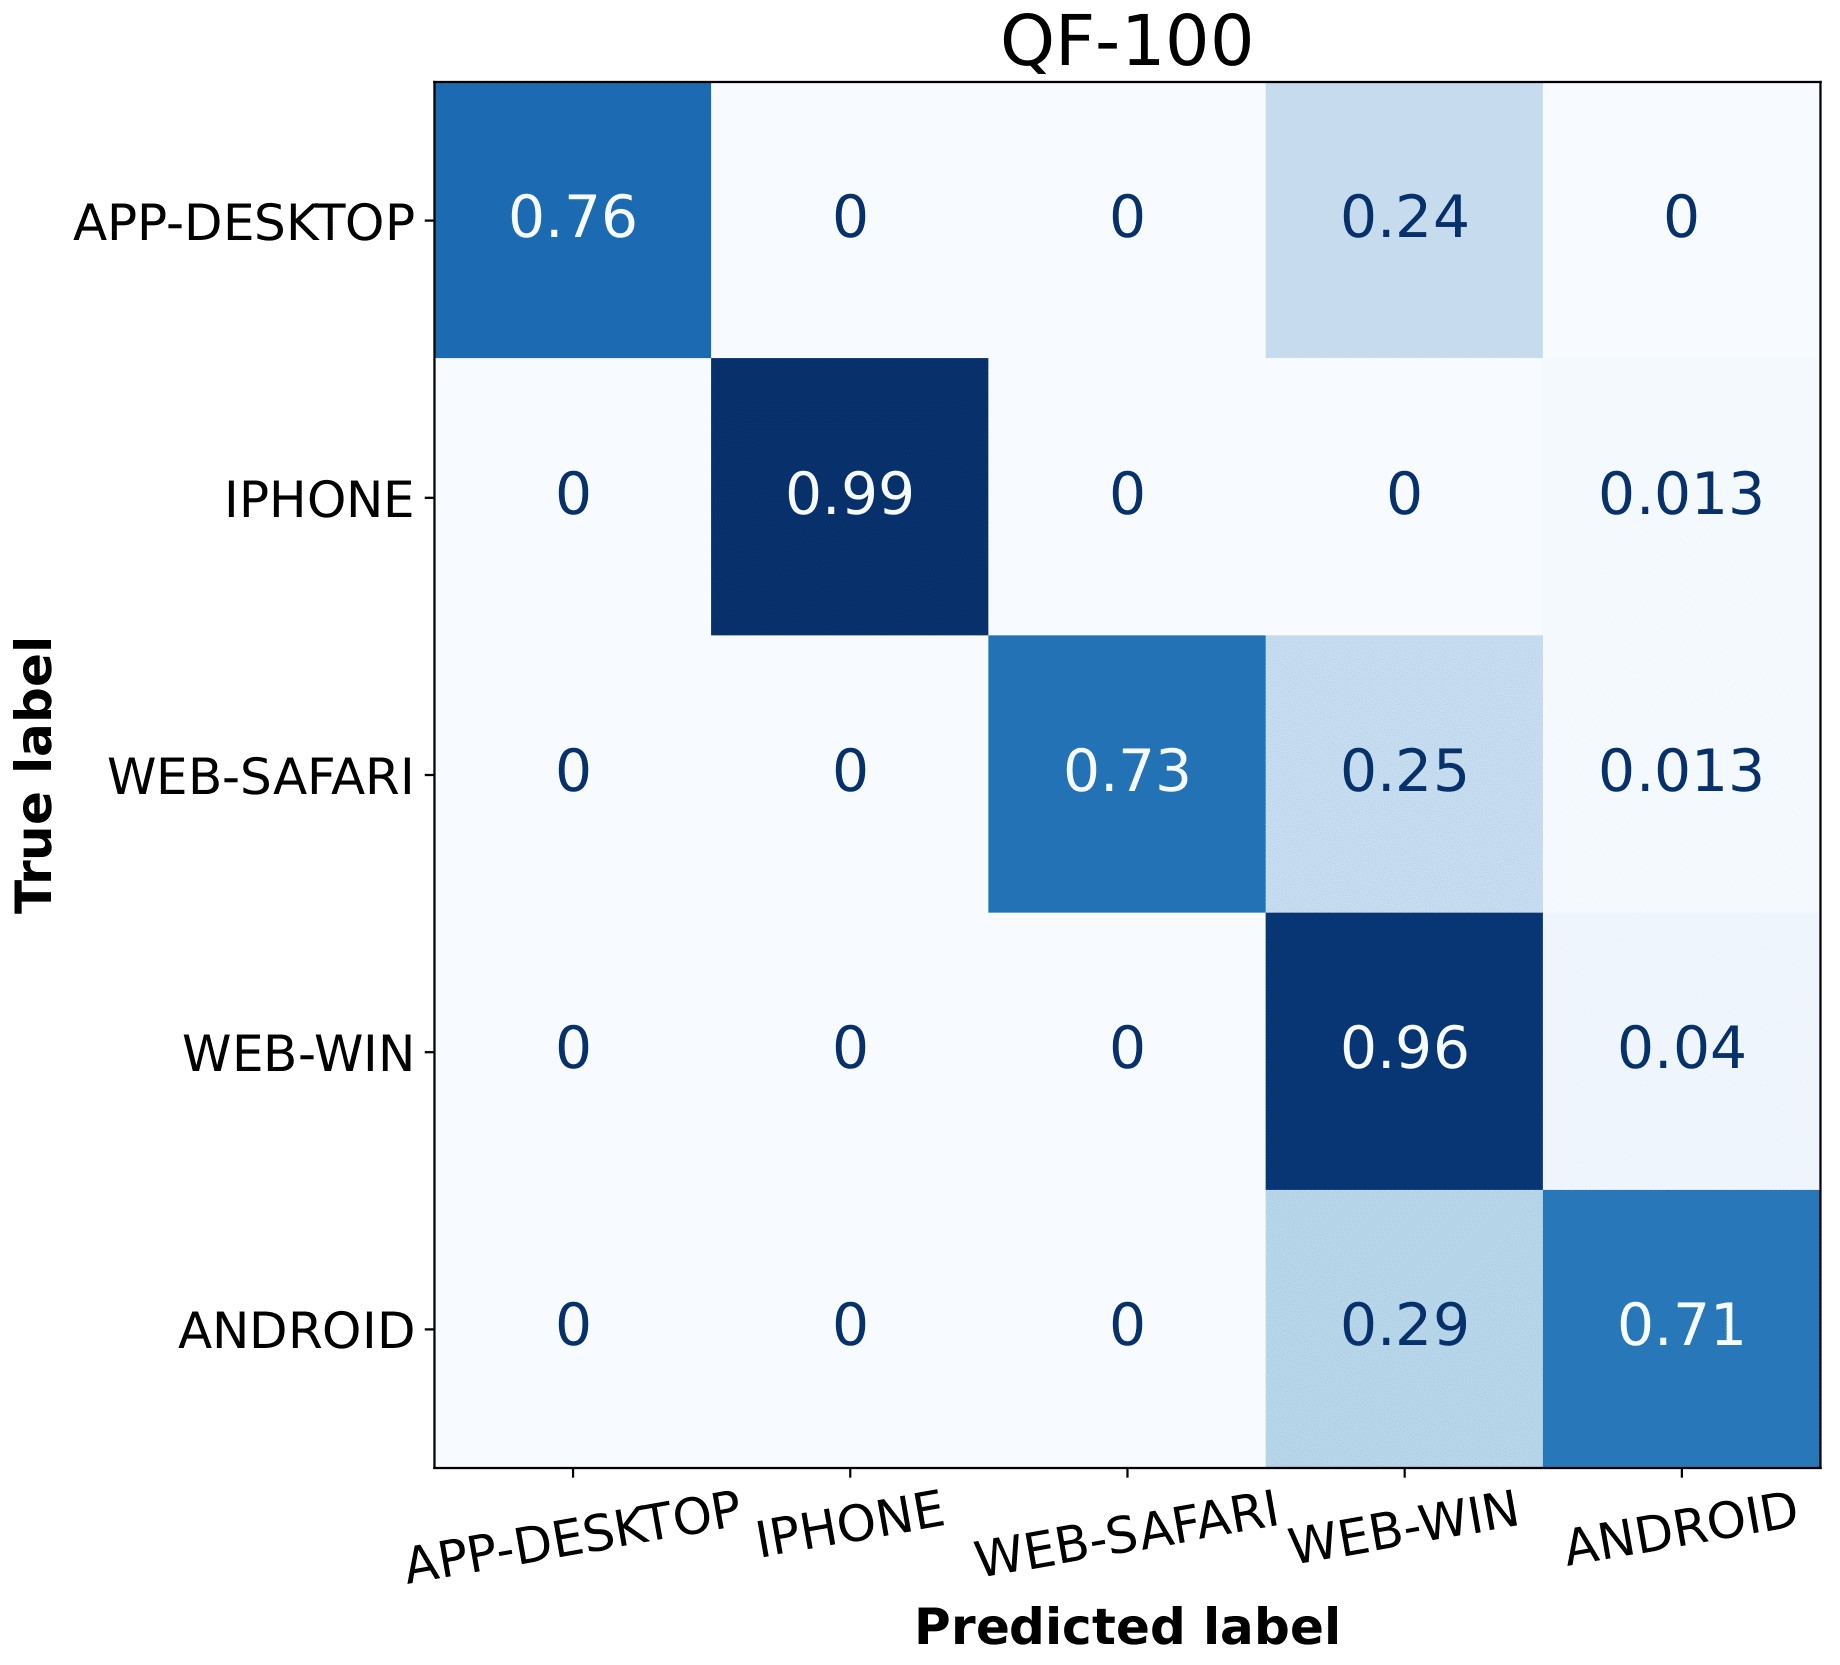
\includegraphics[width=8cm, height=8cm, keepaspectratio]{Immagini/Classificazione/confusion_matrix_SVM_QF-100.jpg}
    \captionof{figure}{\textit{Confusion matrix} per \textit{support vector machine} divise per \textit{quality factor}.}
    \label{fig:class_QF_SVM}
\endgroup

% \begin{figure}[h!]
%     \centering
%     \subfloat[][]{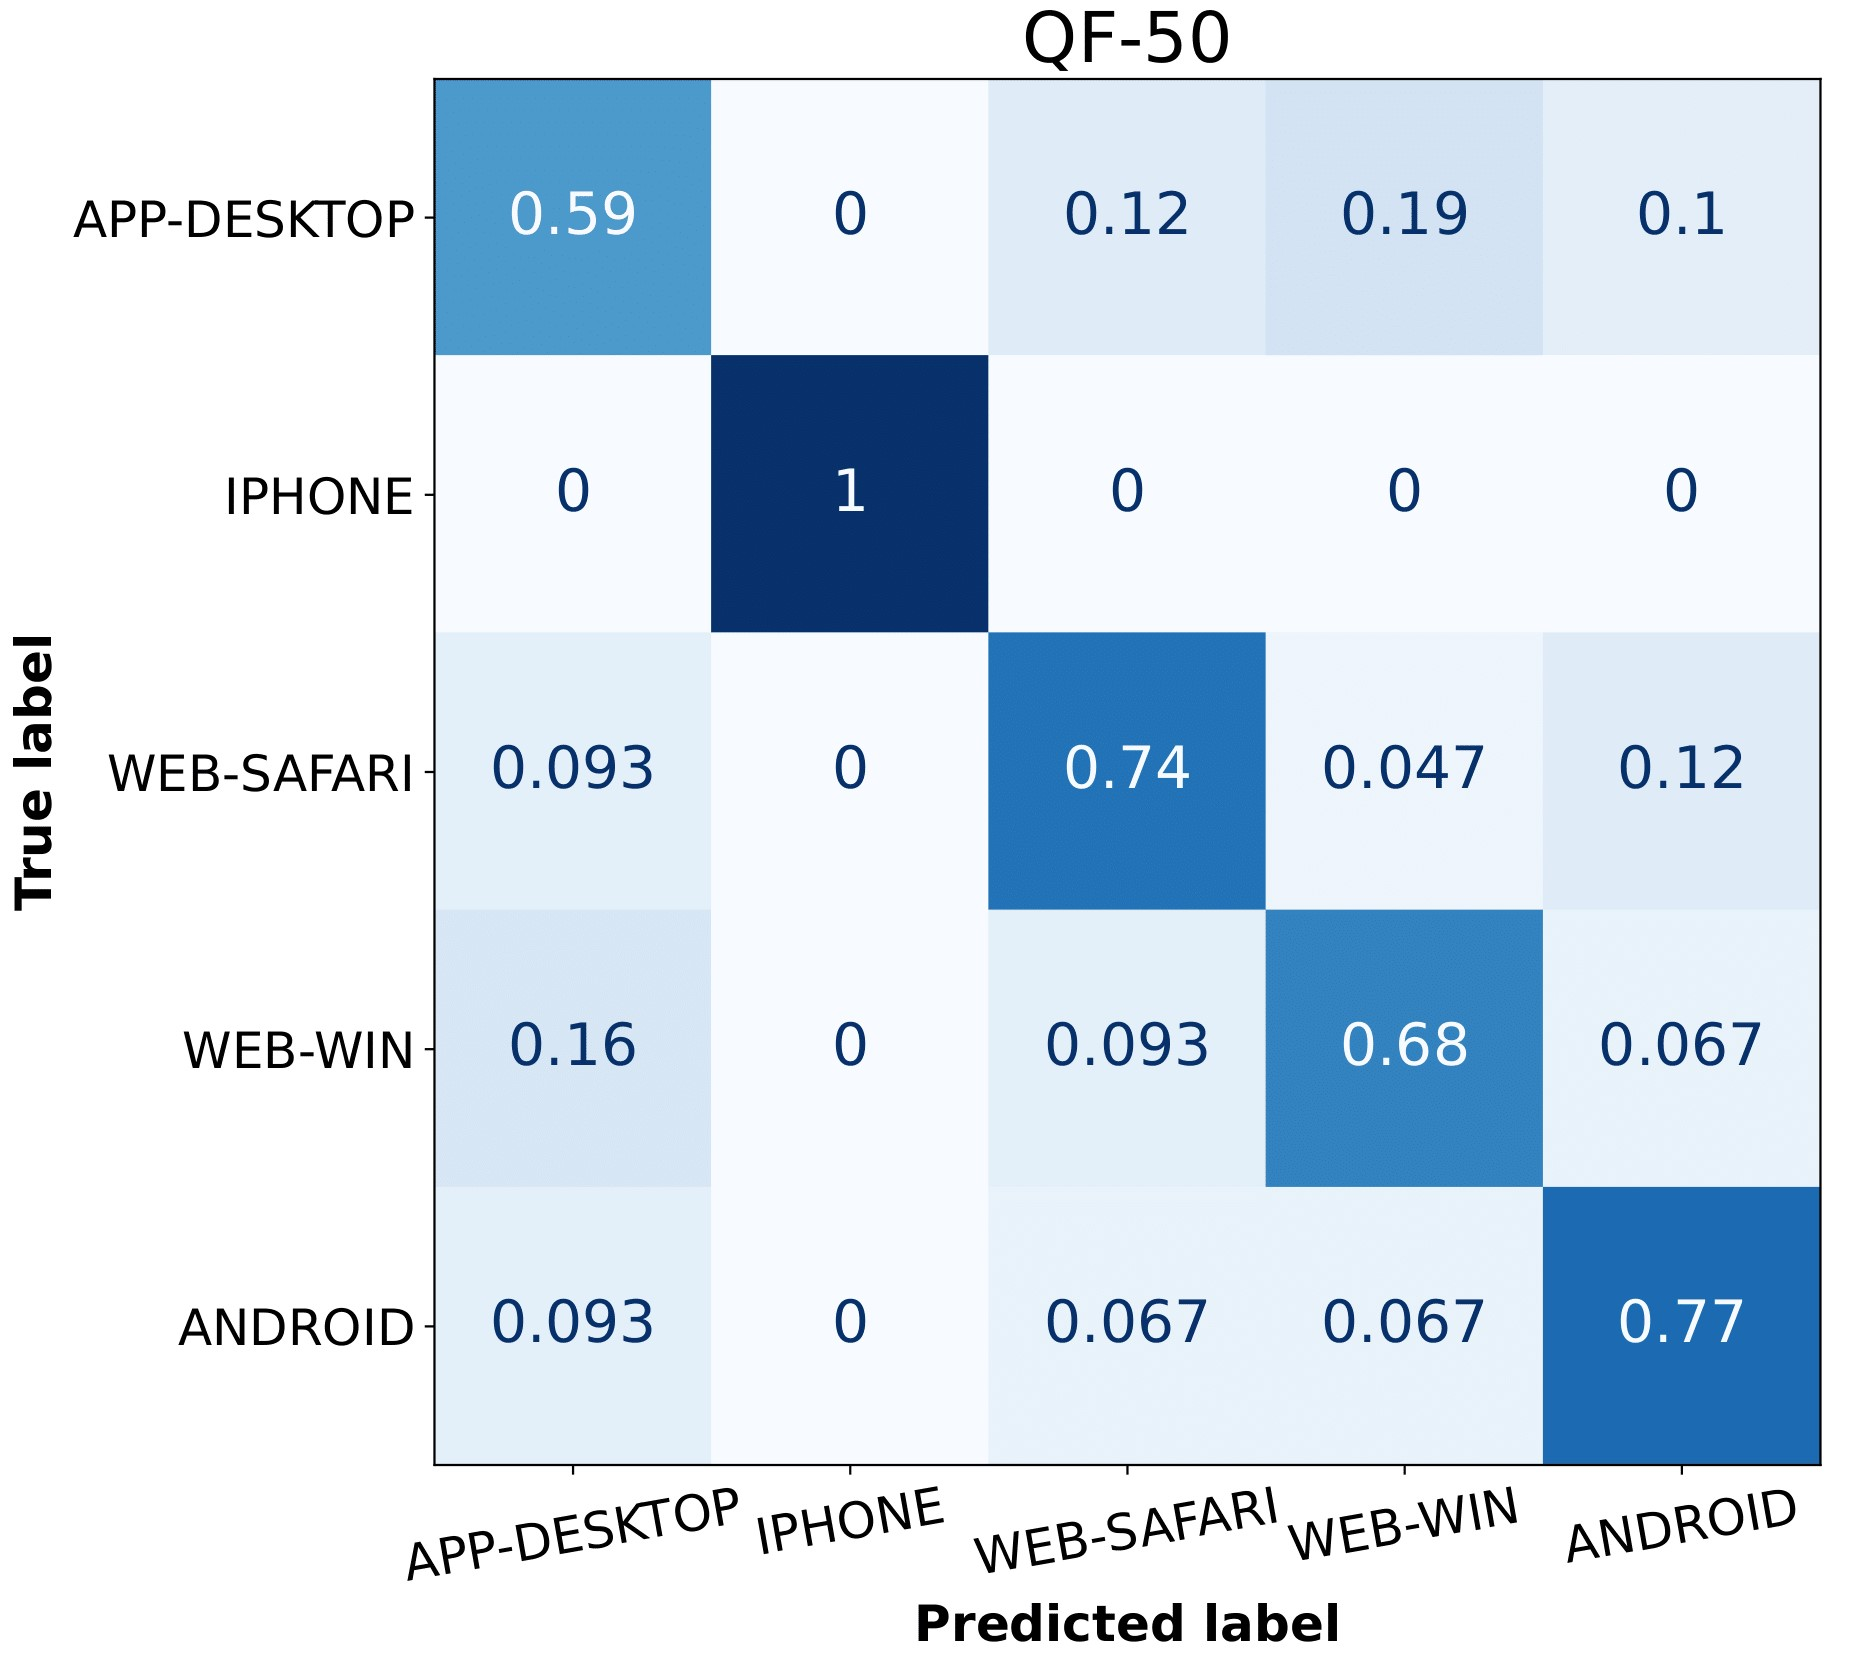
\includegraphics[width=8cm, height=8cm, keepaspectratio]{Immagini/Classificazione/confusion_matrix_RF_QF-50.jpg}}\ \ \ \ \
%     \subfloat[][]{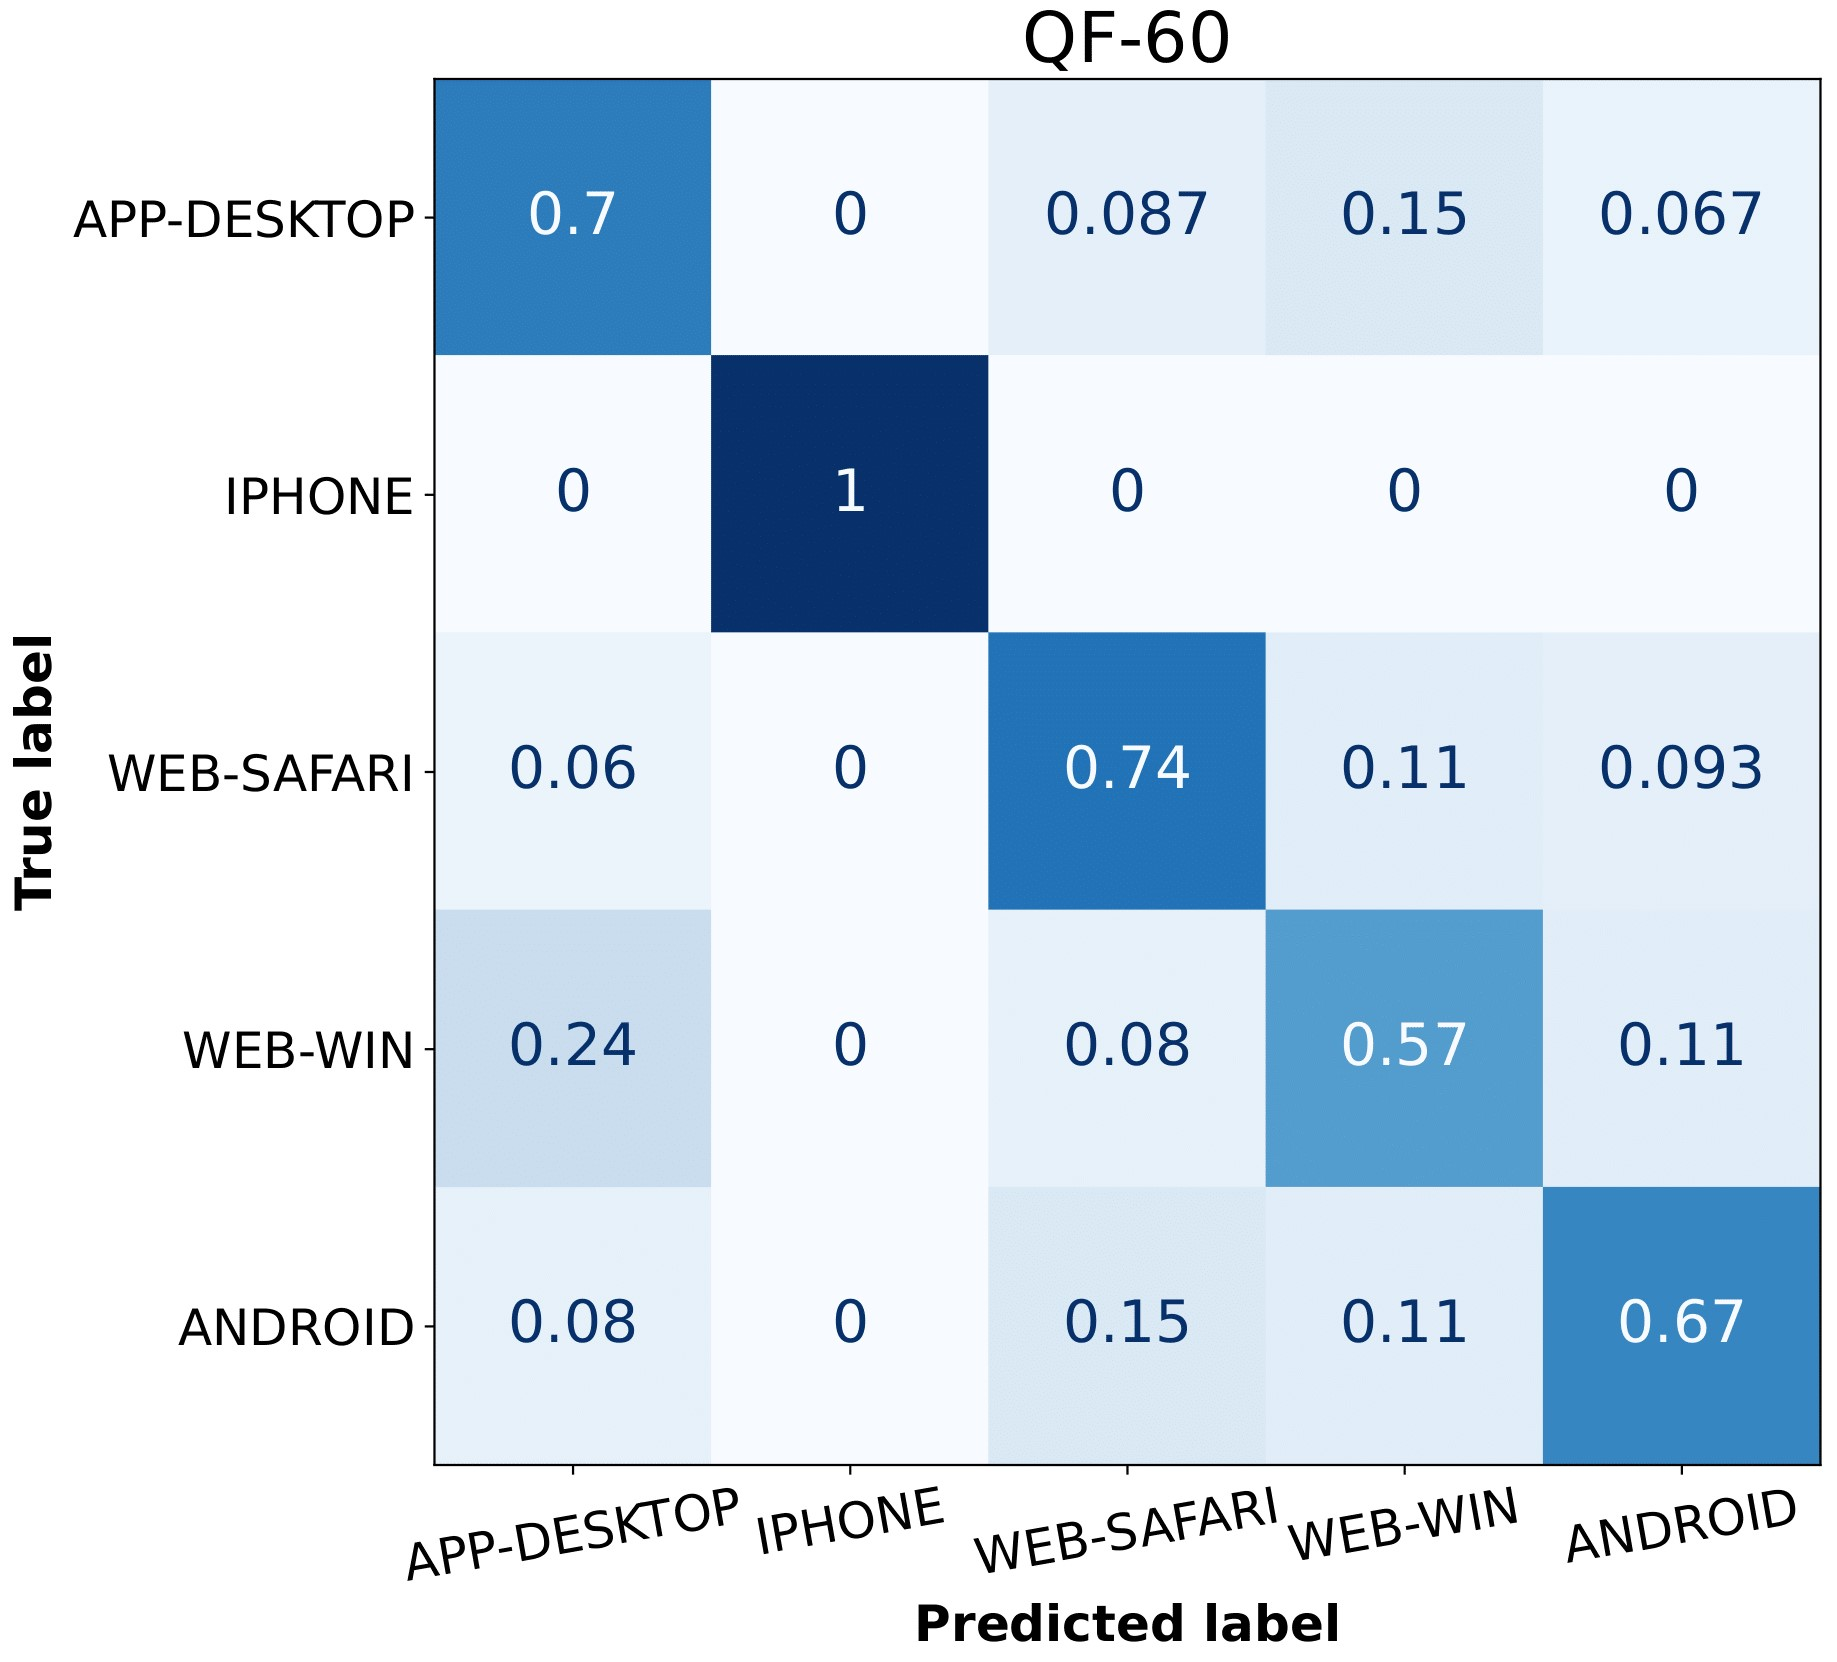
\includegraphics[width=8cm, height=8cm, keepaspectratio]{Immagini/Classificazione/confusion_matrix_RF_QF-60.jpg}}\\
%     \subfloat[][]{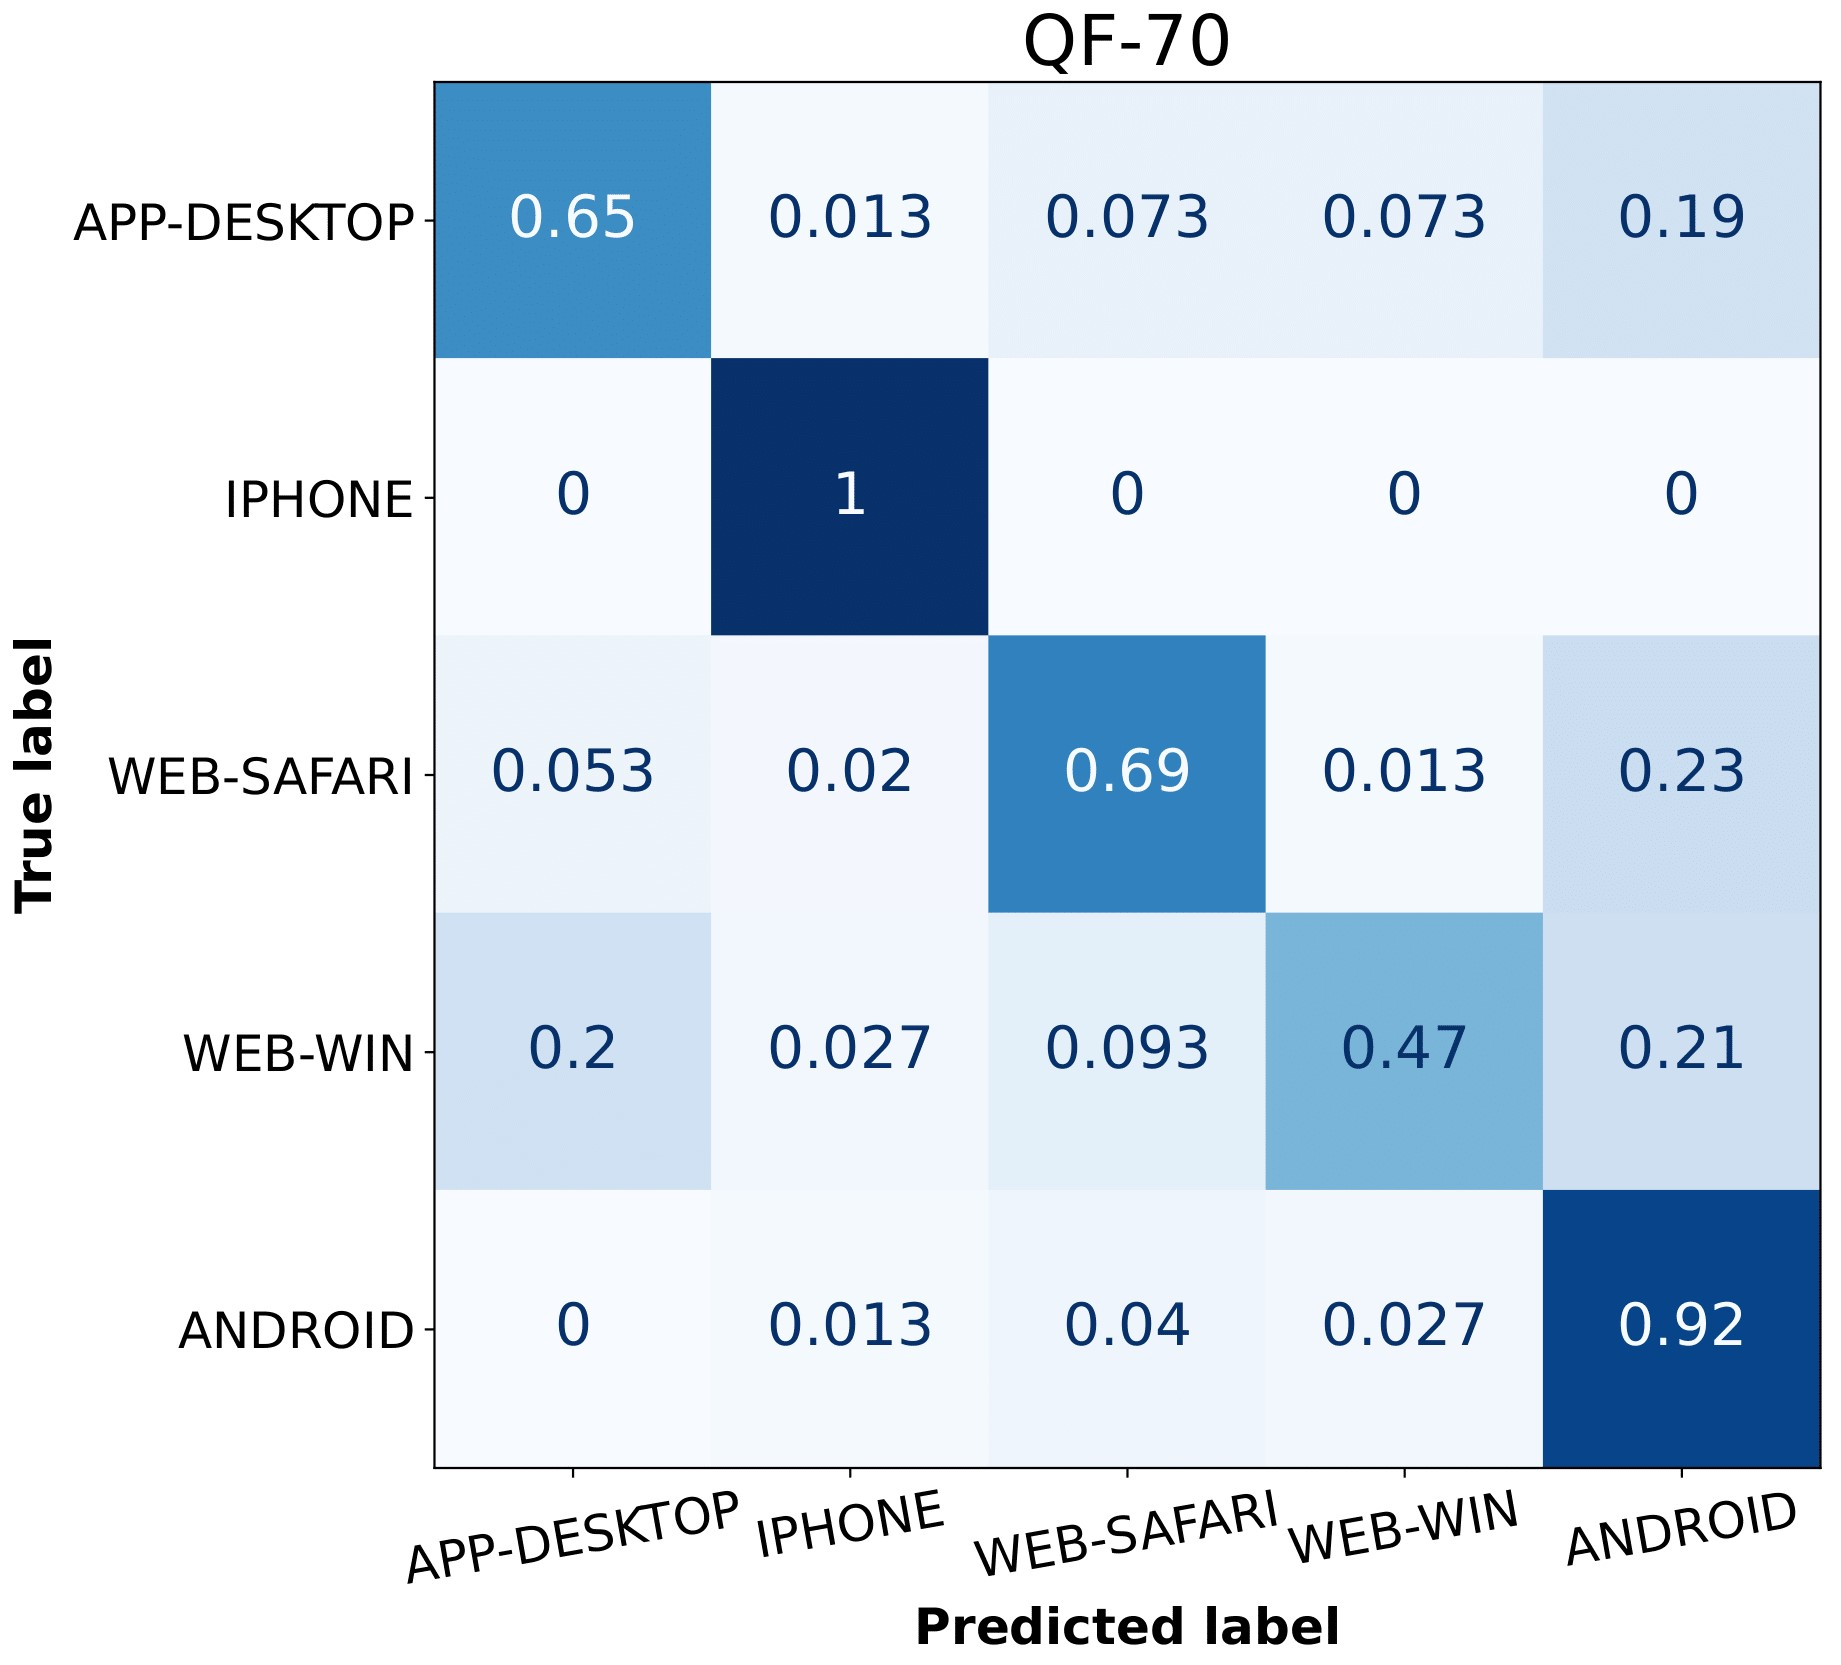
\includegraphics[width=8cm, height=8cm, keepaspectratio]{Immagini/Classificazione/confusion_matrix_RF_QF-70.jpg}}\ \ \ \ \
%     \subfloat[][]{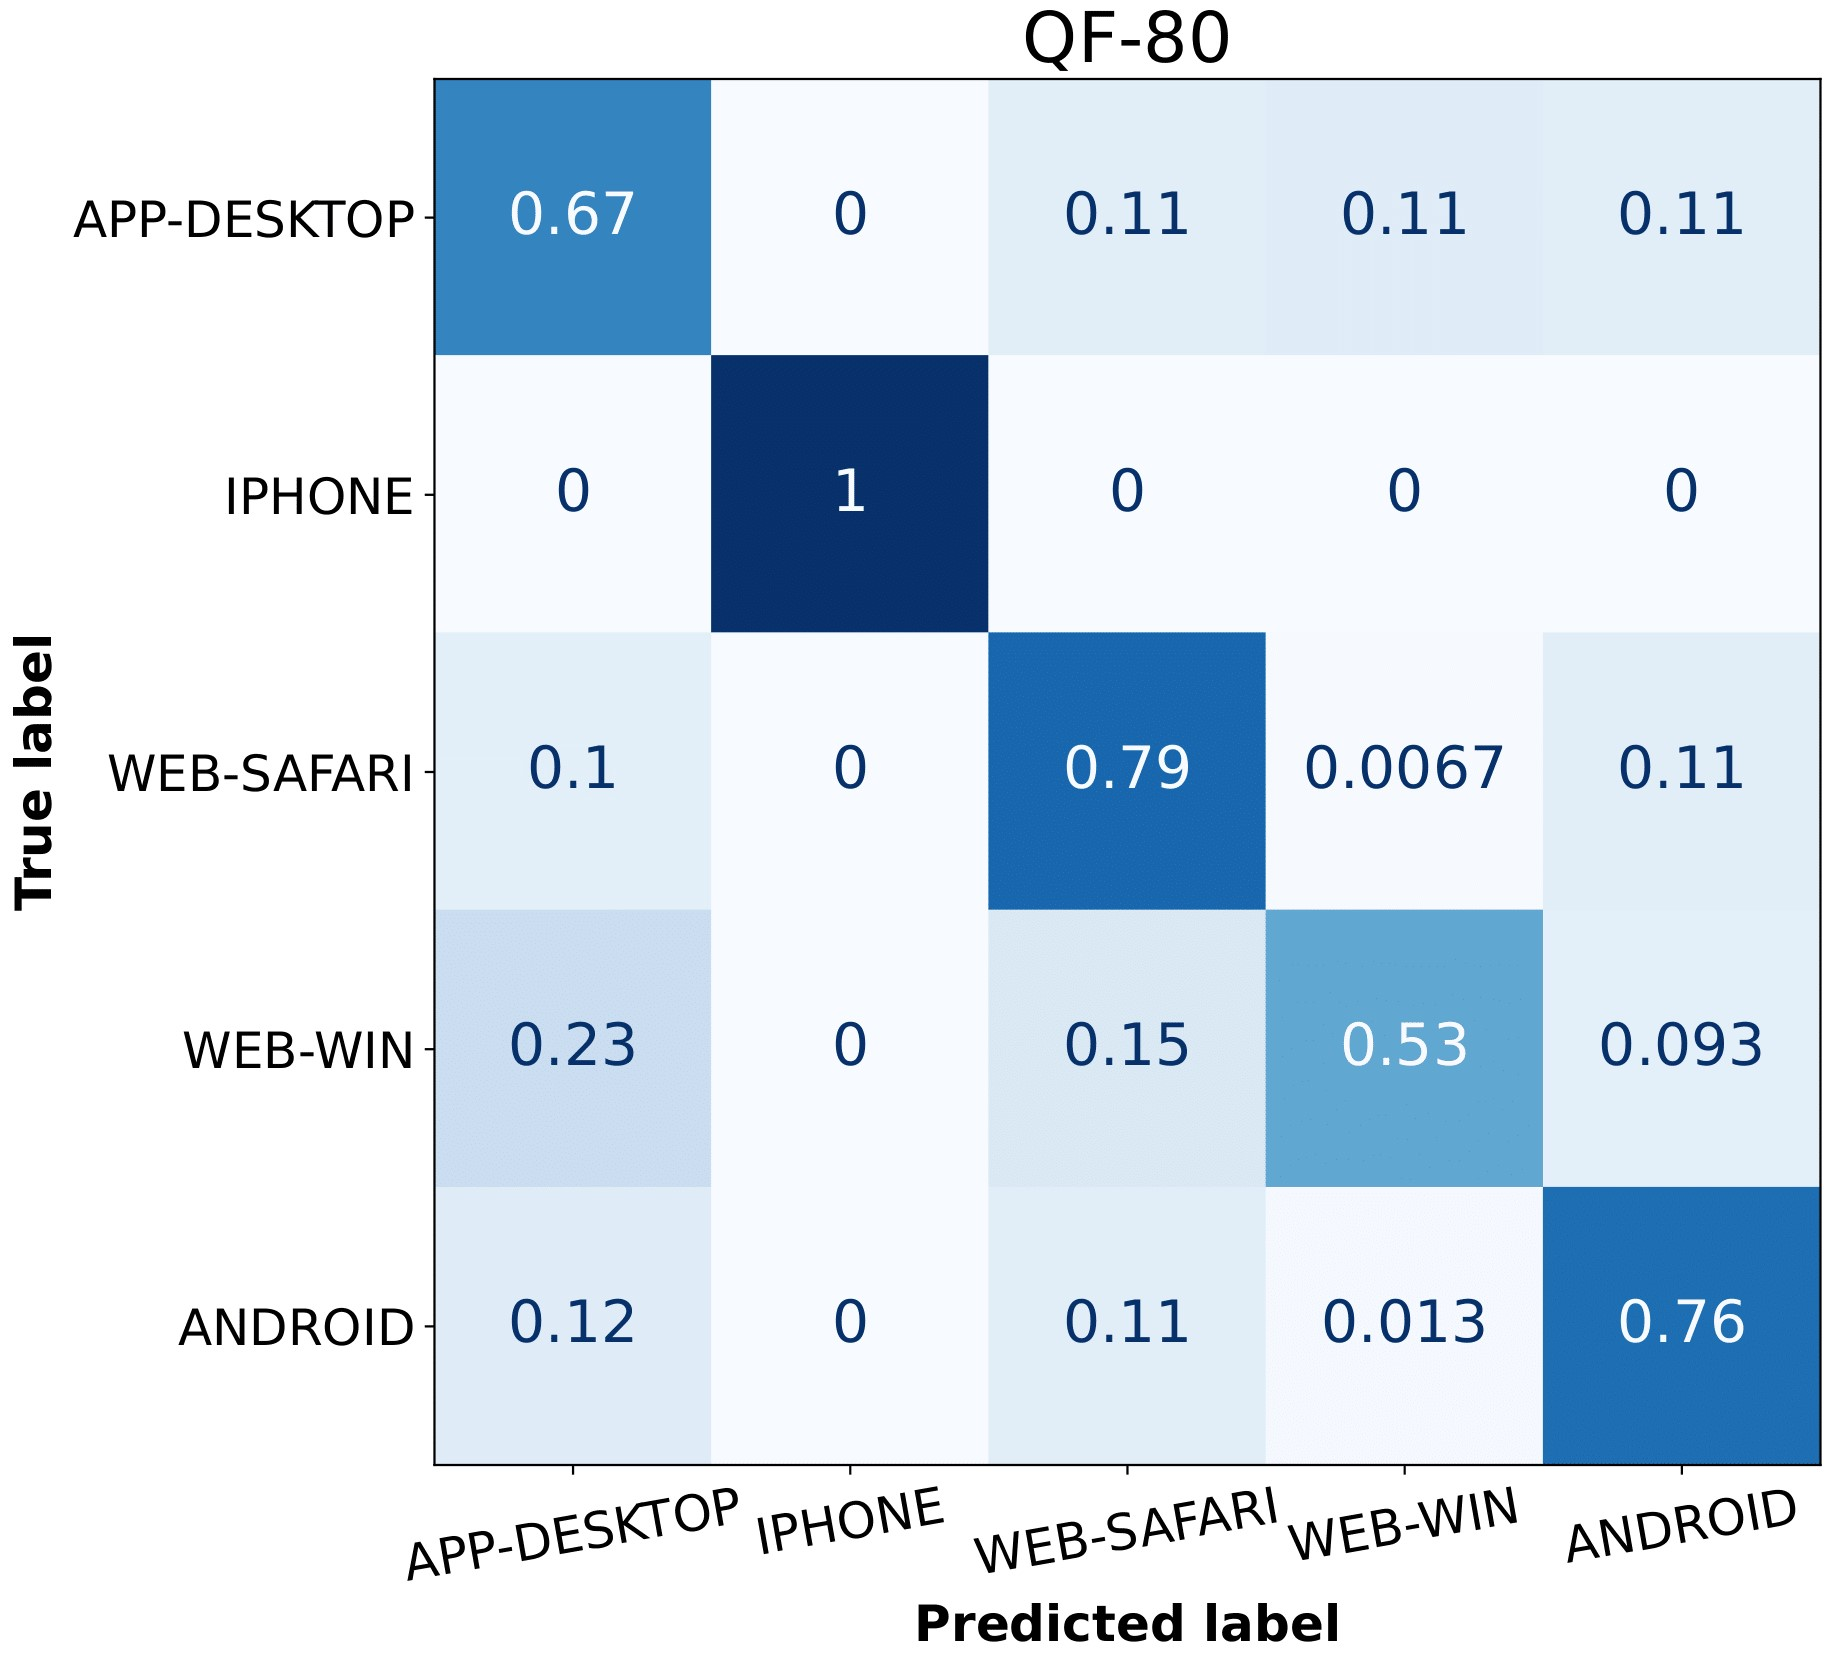
\includegraphics[width=8cm, height=8cm, keepaspectratio]{Immagini/Classificazione/confusion_matrix_RF_QF-80.jpg}}\\
%     \subfloat[][]{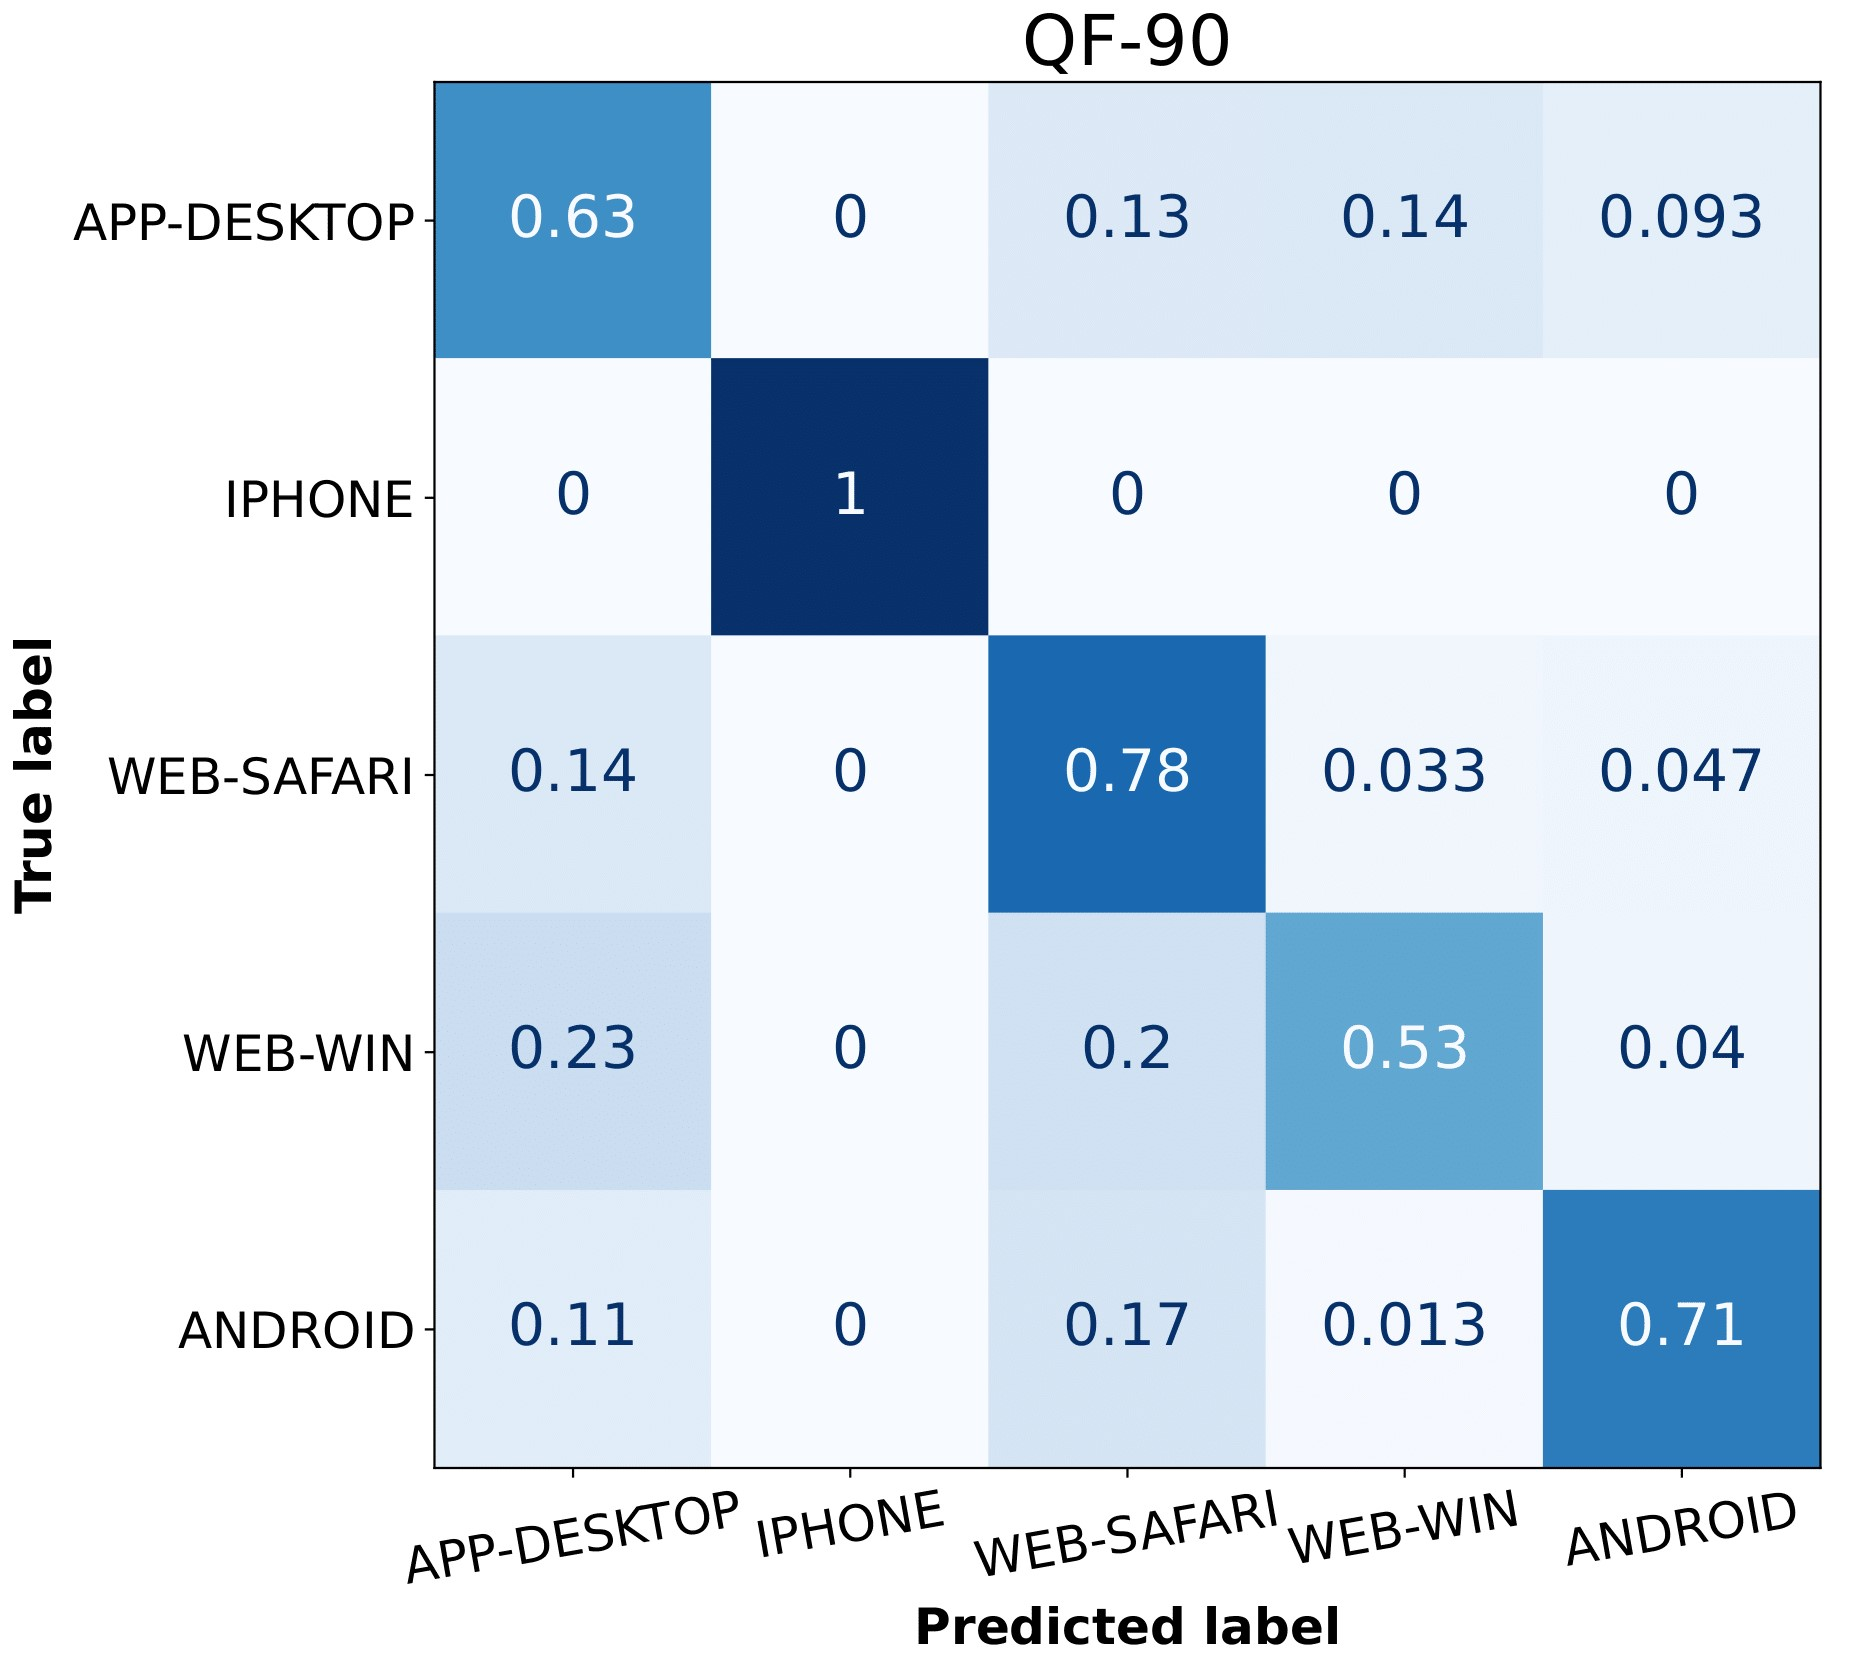
\includegraphics[width=8cm, height=8cm, keepaspectratio]{Immagini/Classificazione/confusion_matrix_RF_QF-90.jpg}}\ \ \ \ \
%     \subfloat[][]{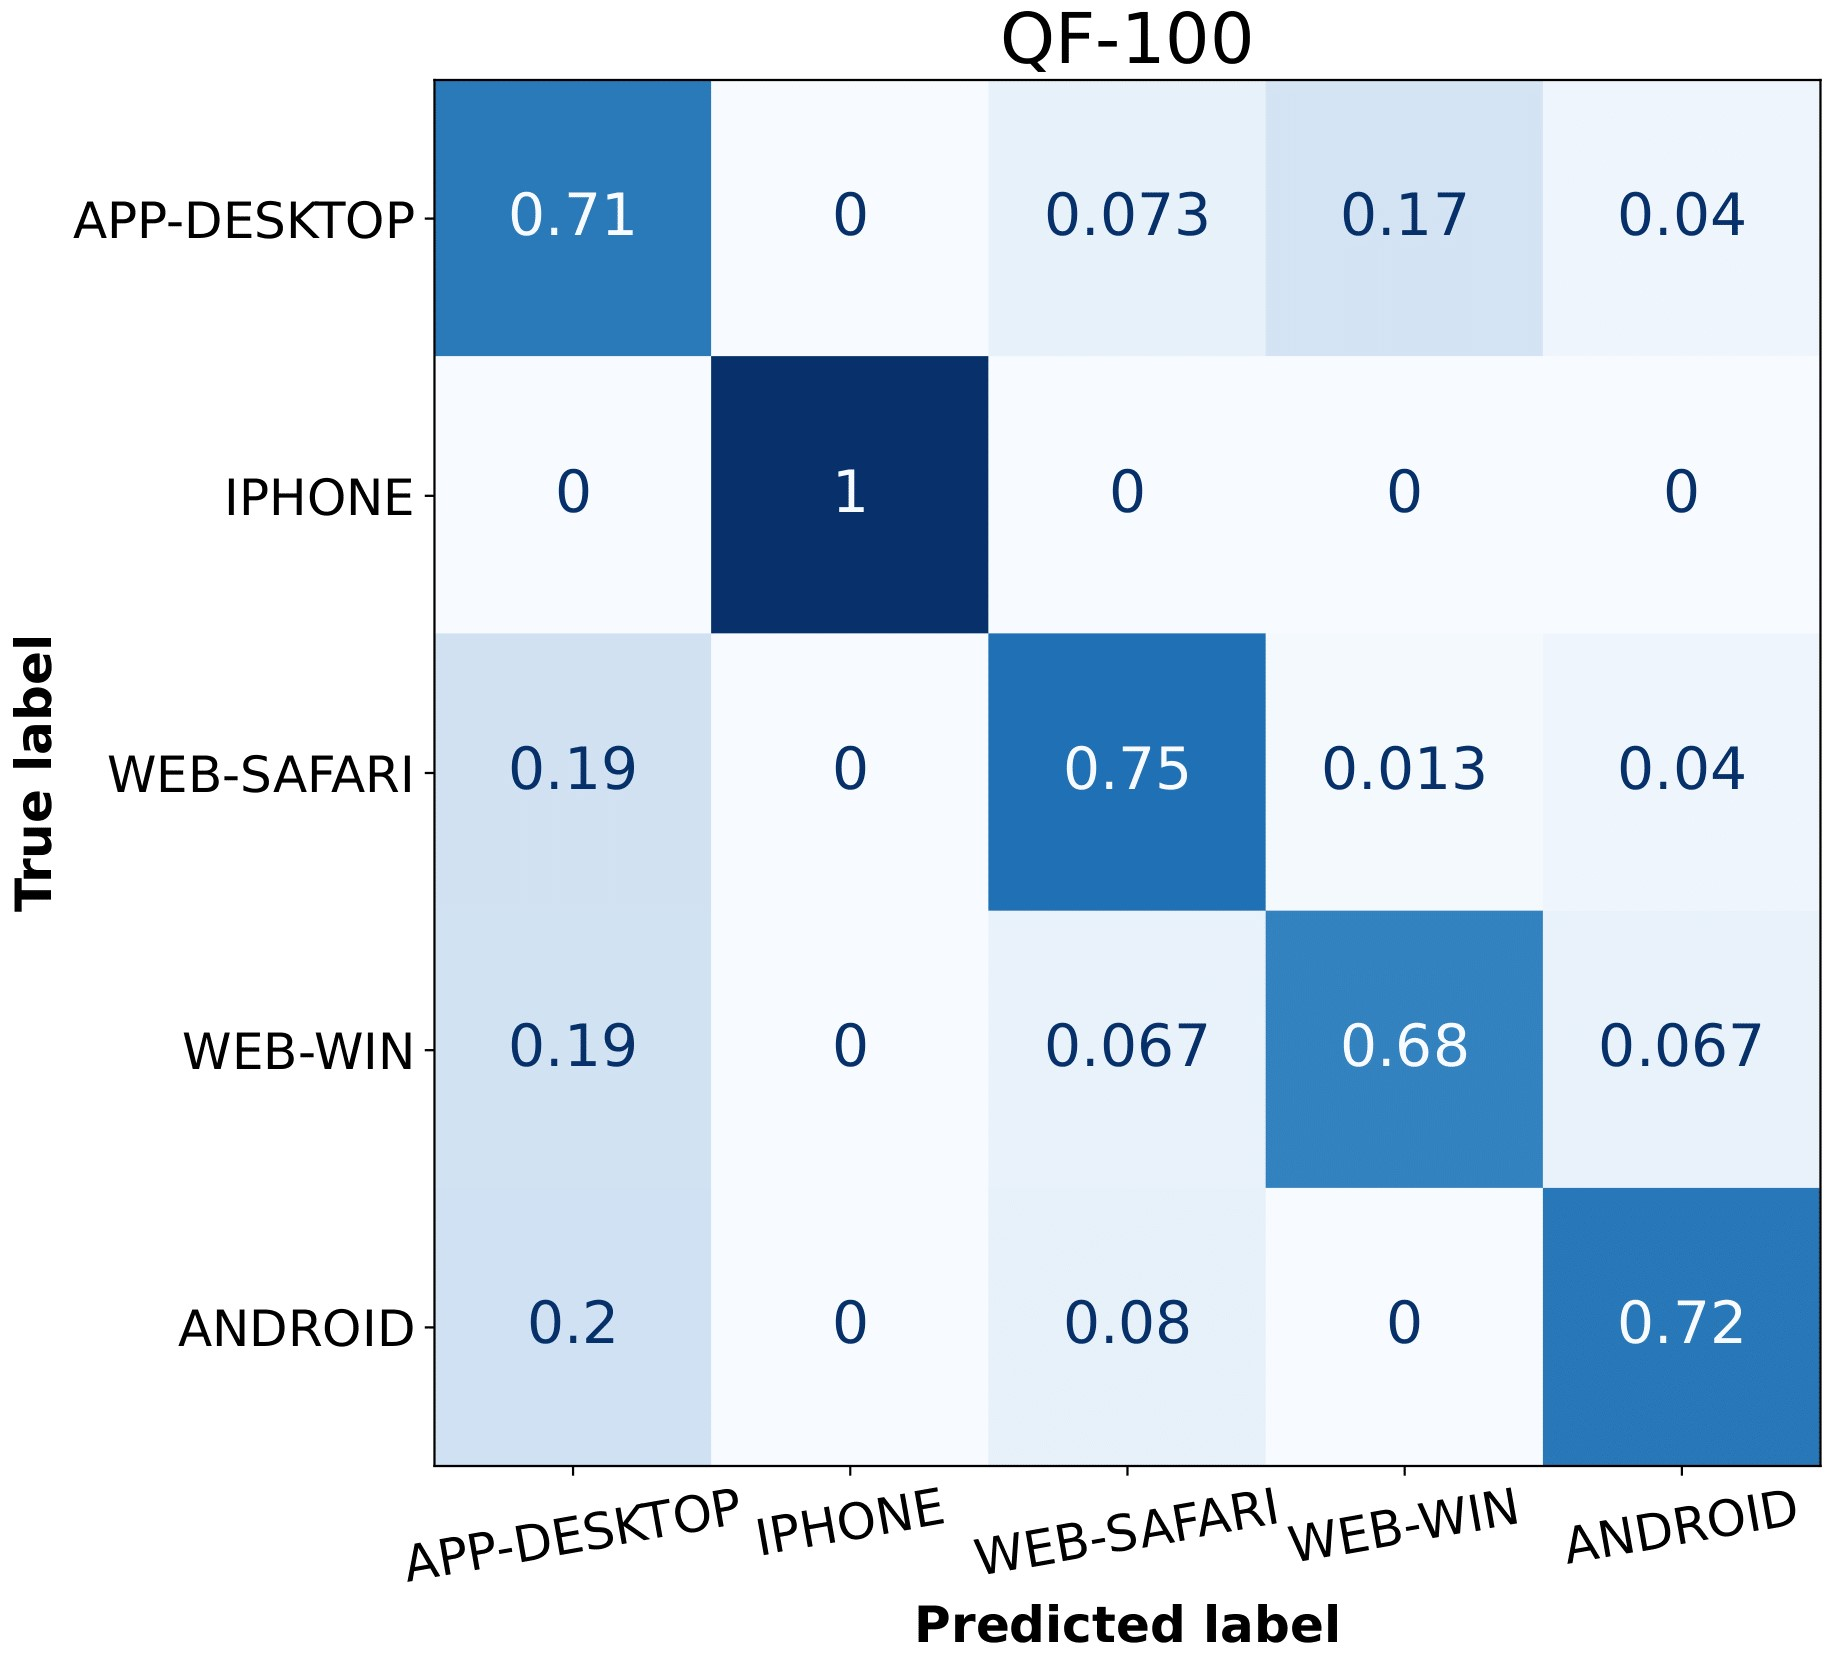
\includegraphics[width=8cm, height=8cm, keepaspectratio]{Immagini/Classificazione/confusion_matrix_RF_QF-100.jpg}}
%     \caption{\textit{Confusion matrix} per \textit{random forest} divise per \textit{quality factor}.}
%     \label{fig:class_QF_RF}
% \end{figure}

% \begin{figure}[h!]
%     \centering
%     \subfloat[][]{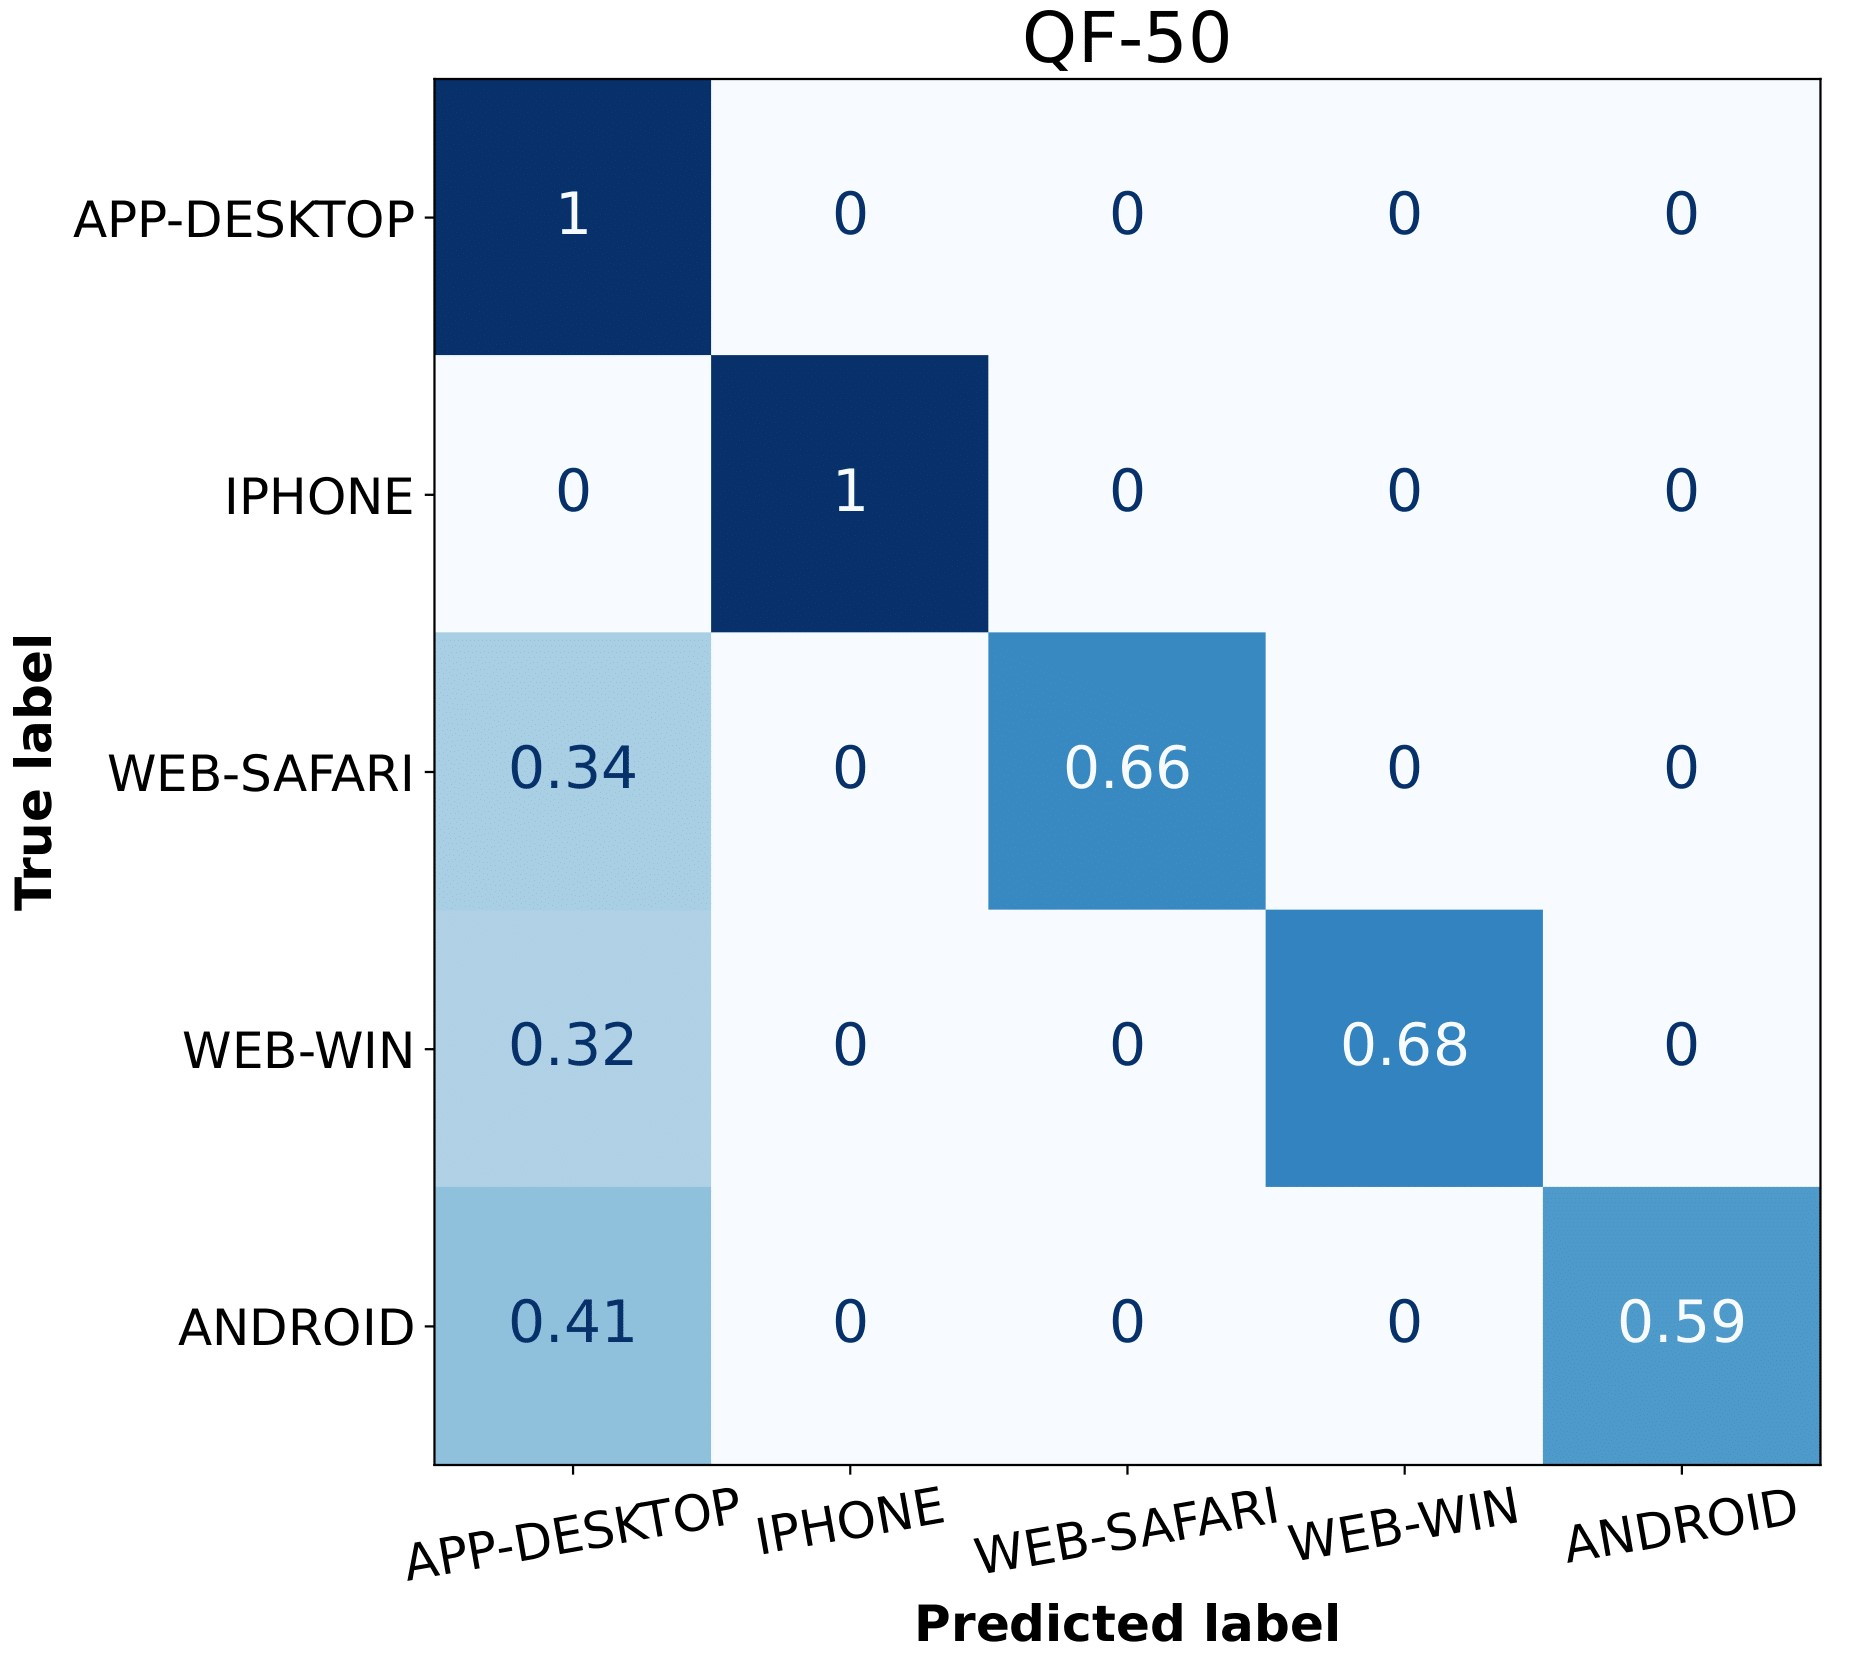
\includegraphics[width=8cm, height=8cm, keepaspectratio]{Immagini/Classificazione/confusion_matrix_SVM_QF-50.jpg}}\ \ \ \ \
%     \subfloat[][]{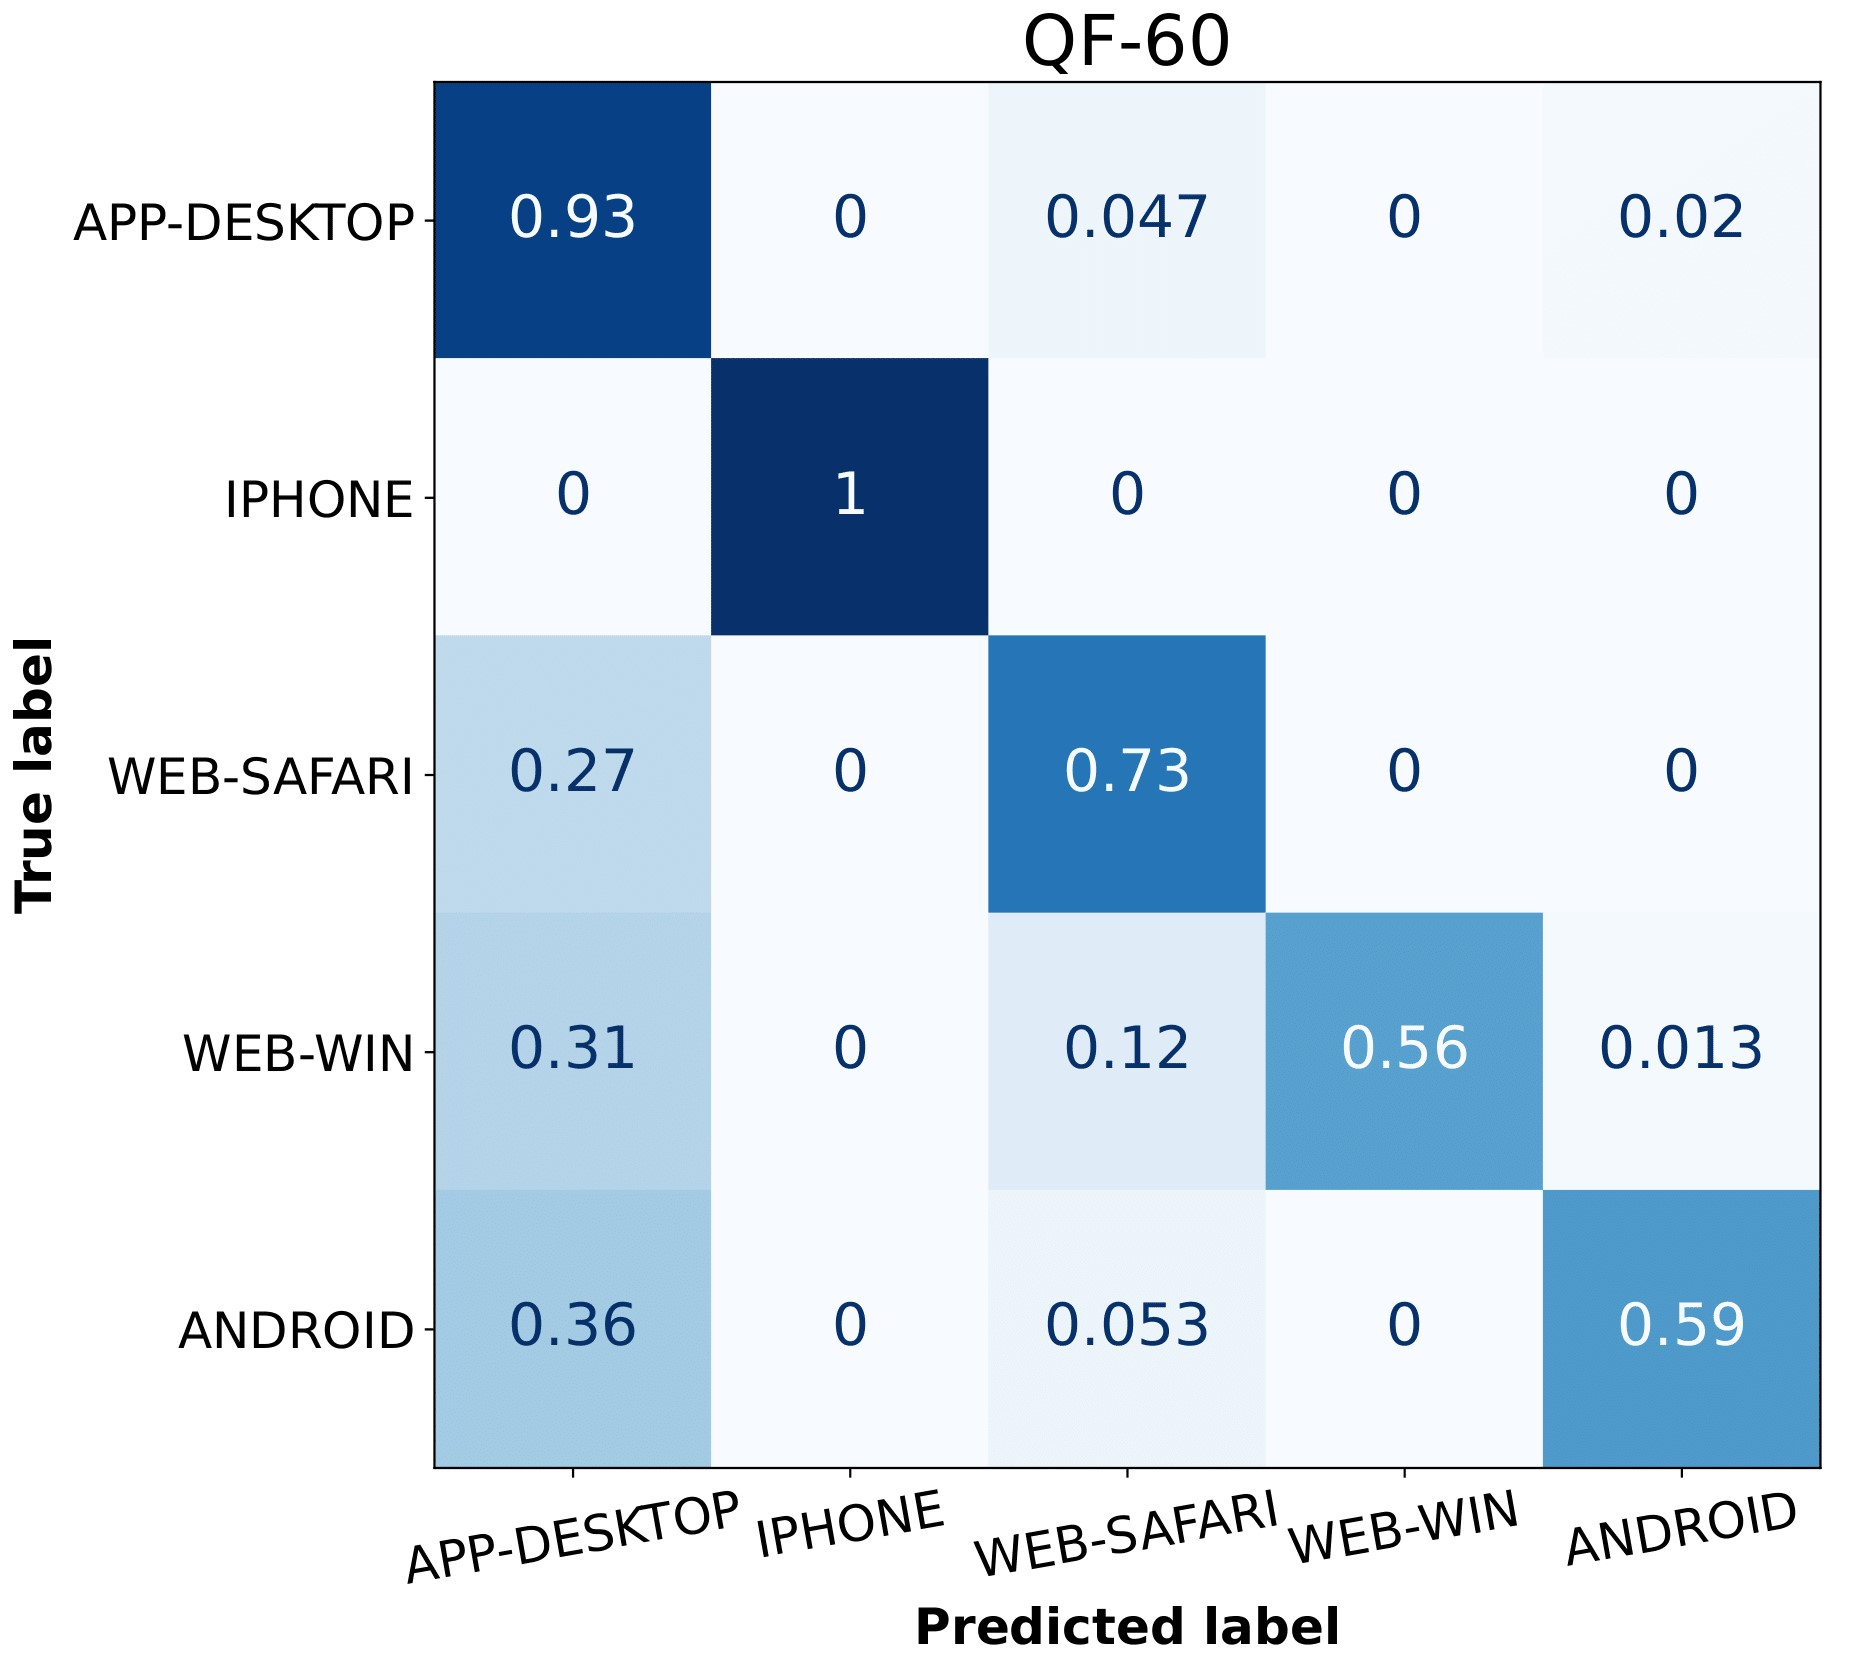
\includegraphics[width=8cm, height=8cm, keepaspectratio]{Immagini/Classificazione/confusion_matrix_SVM_QF-60.jpg}}\\
%     \subfloat[][]{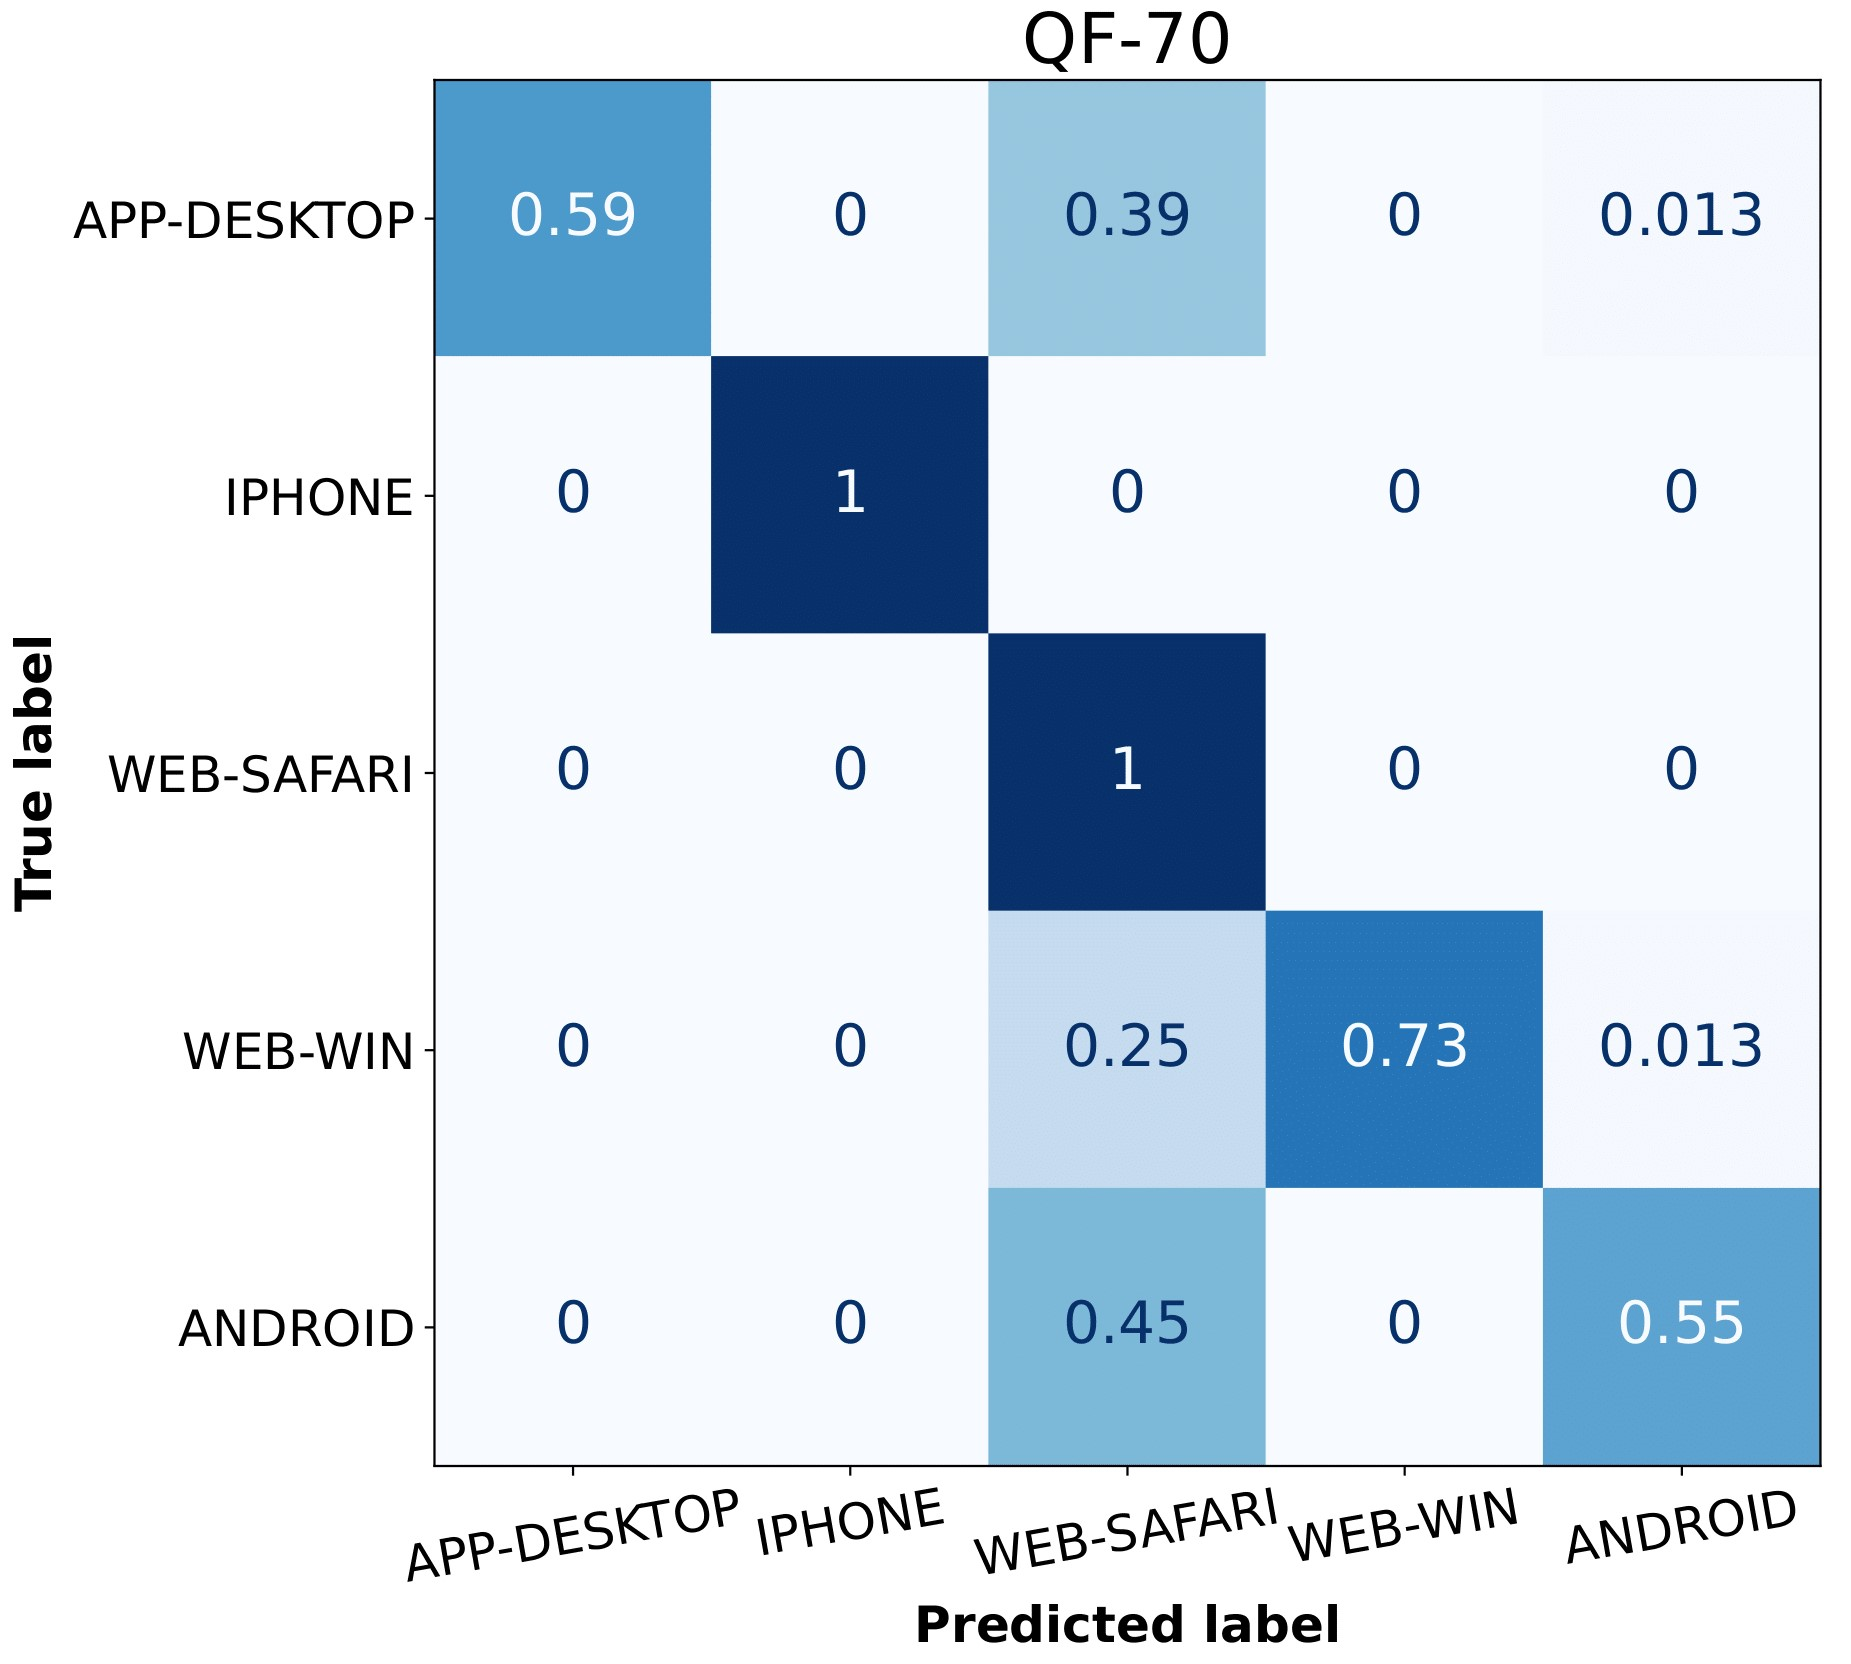
\includegraphics[width=8cm, height=8cm, keepaspectratio]{Immagini/Classificazione/confusion_matrix_SVM_QF-70.jpg}}\ \ \ \ \
%     \subfloat[][]{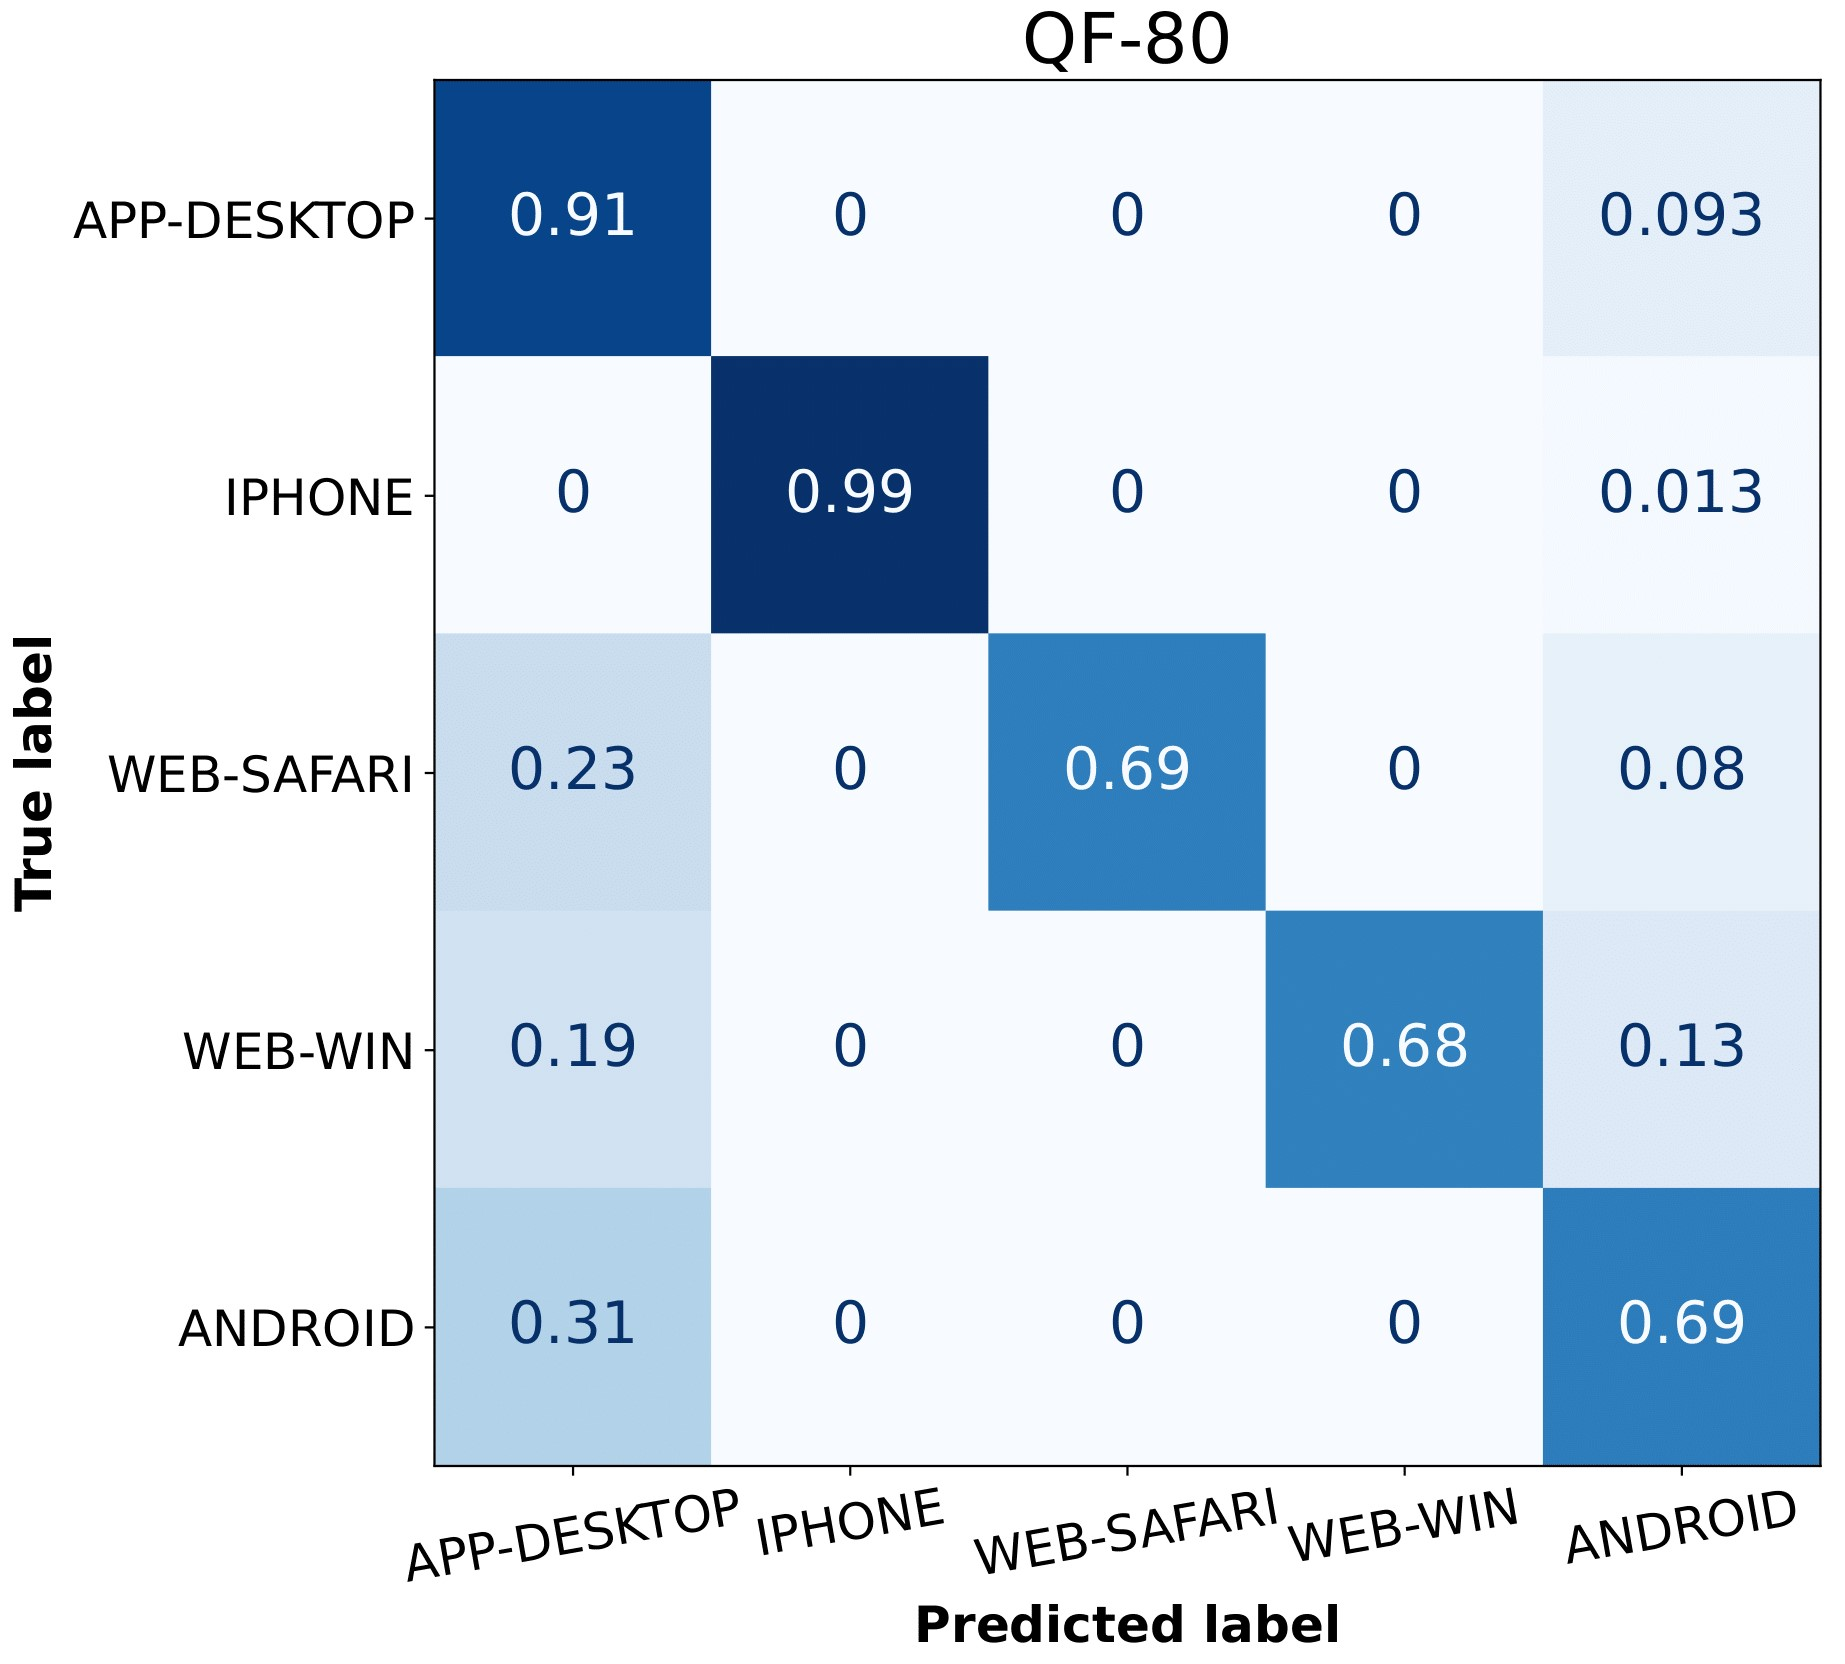
\includegraphics[width=8cm, height=8cm, keepaspectratio]{Immagini/Classificazione/confusion_matrix_SVM_QF-80.jpg}}\\
%     \subfloat[][]{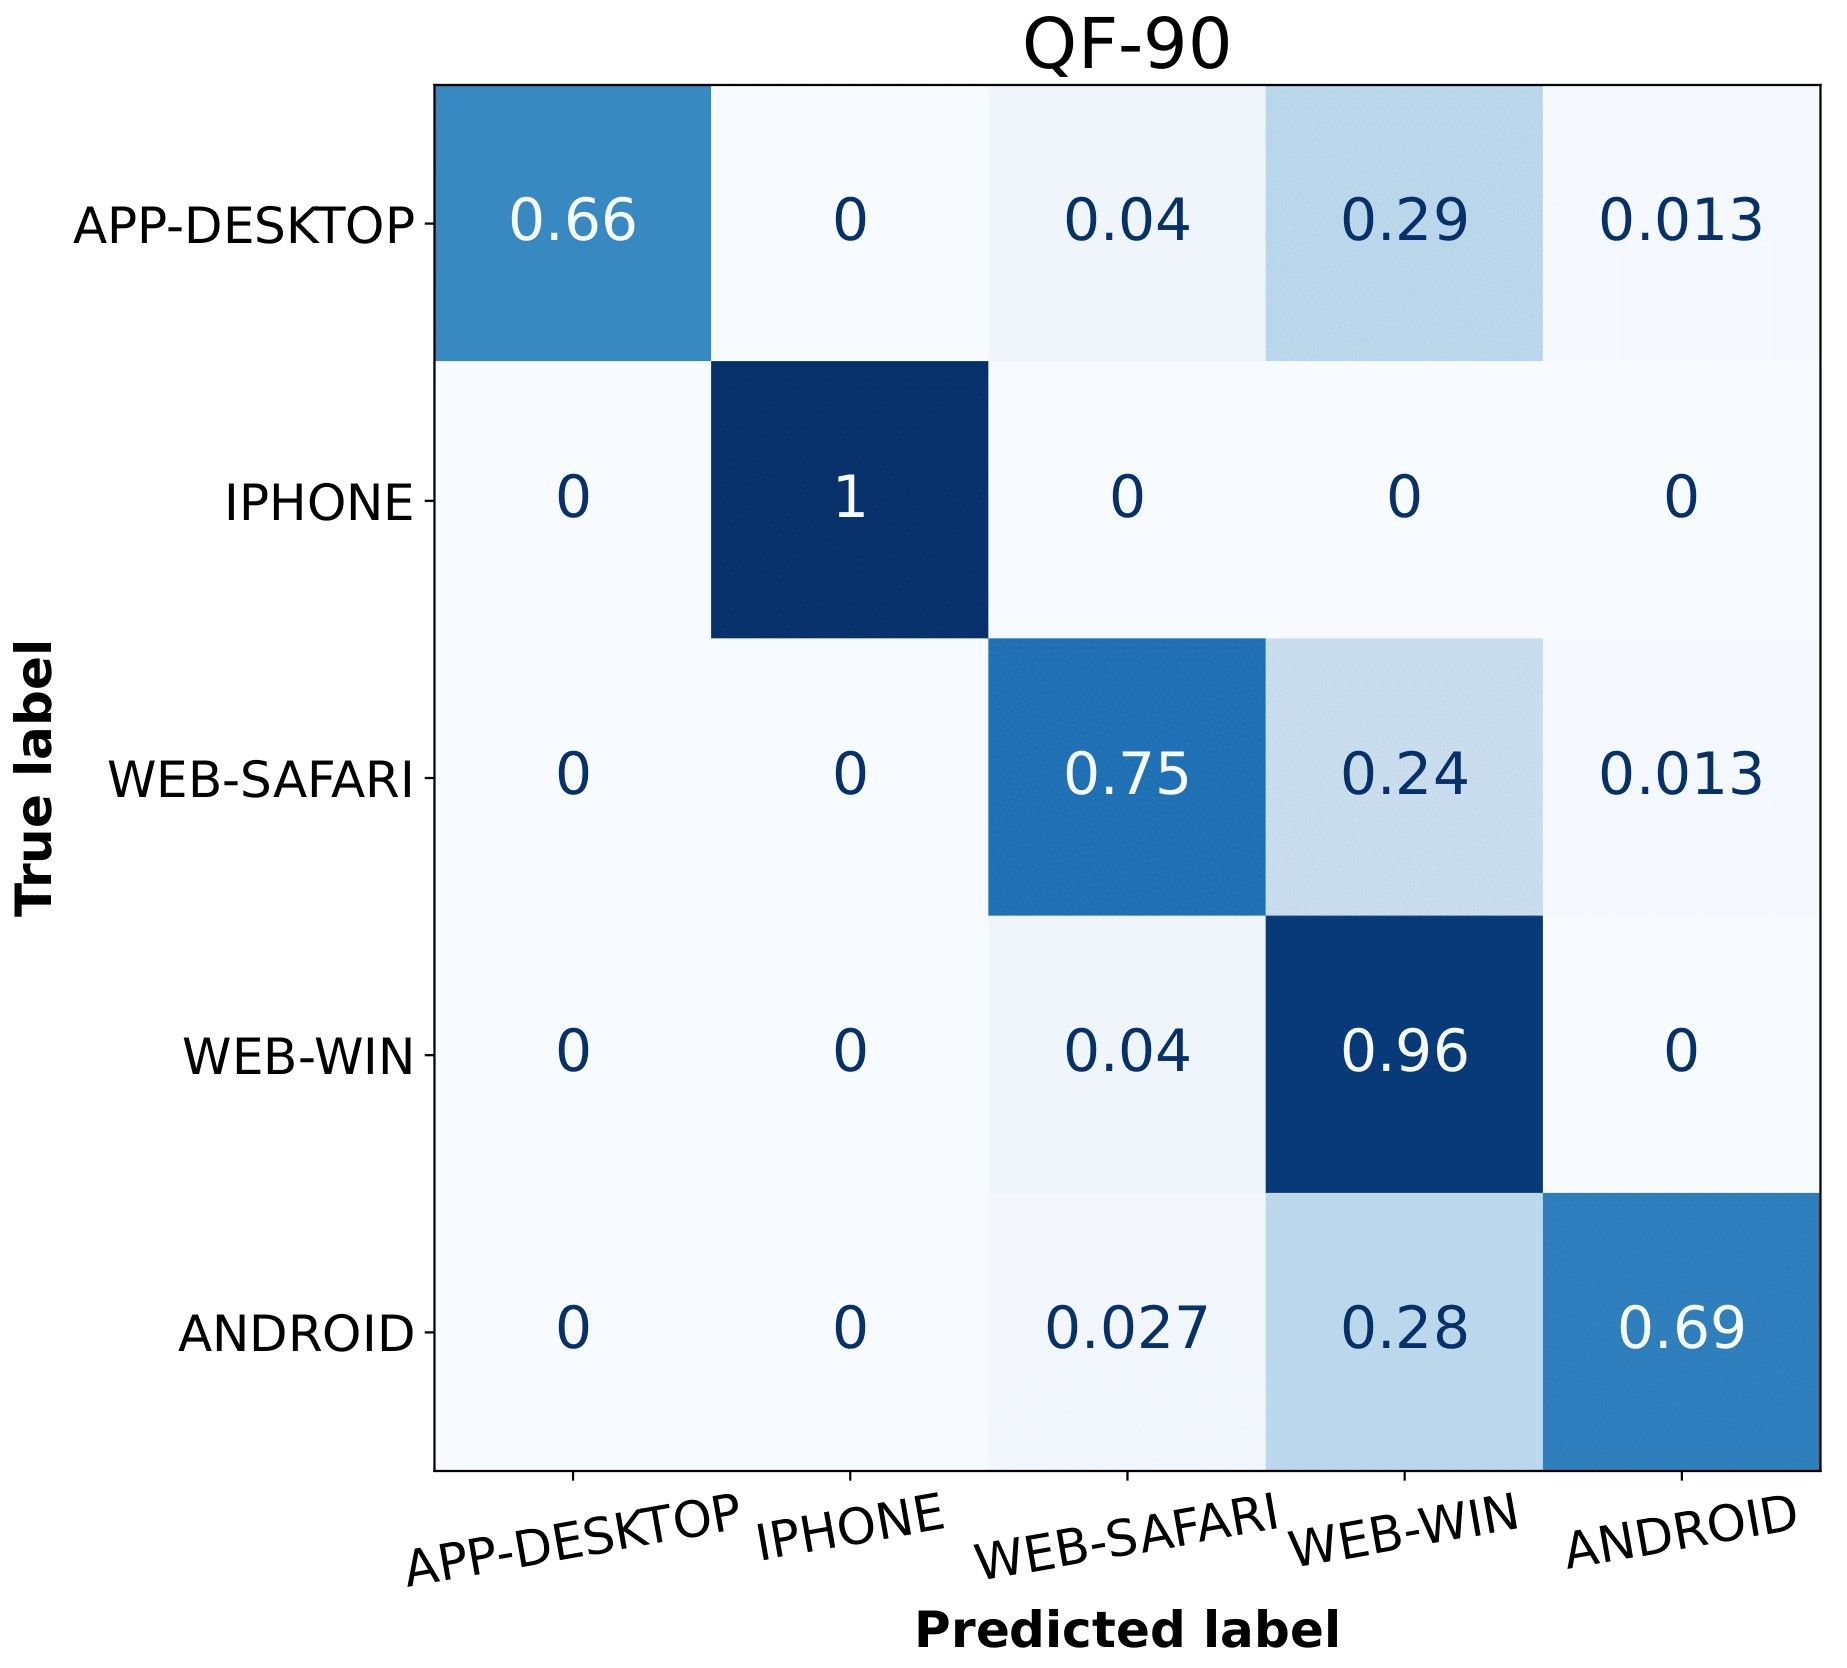
\includegraphics[width=8cm, height=8cm, keepaspectratio]{Immagini/Classificazione/confusion_matrix_SVM_QF-90.jpg}}\ \ \ \ \
%     \subfloat[][]{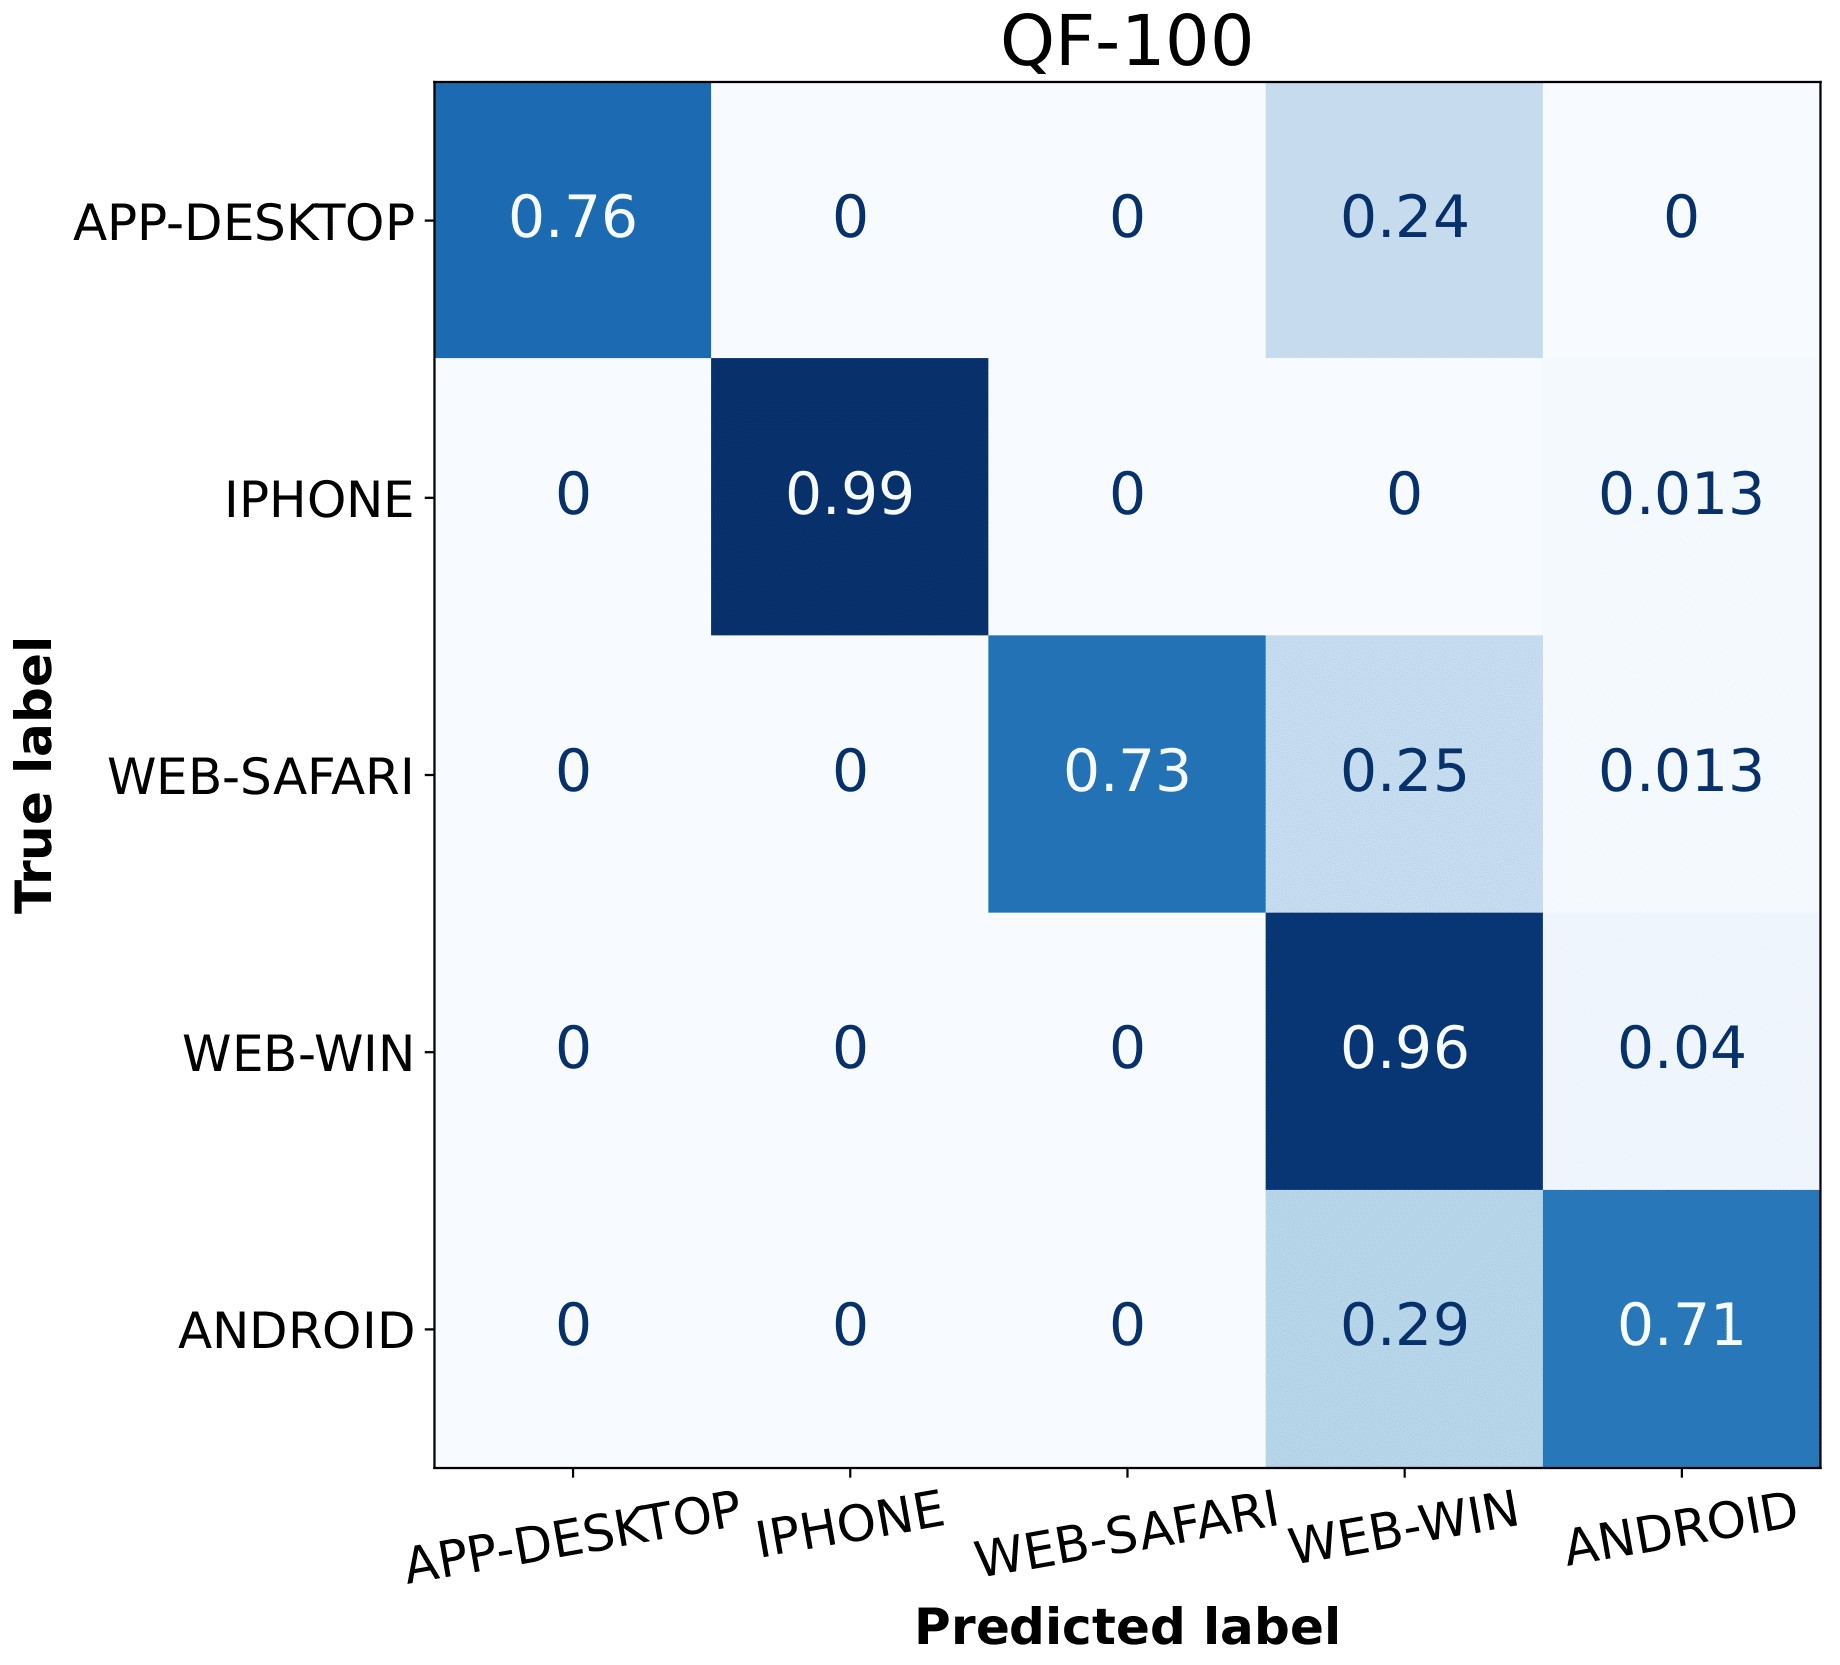
\includegraphics[width=8cm, height=8cm, keepaspectratio]{Immagini/Classificazione/confusion_matrix_SVM_QF-100.jpg}}
%     \caption{\textit{Confusion matrix} per \textit{support vector machine} divise per \textit{quality factor}.}
%     \label{fig:class_QF_SVM}
% \end{figure}

\vspace{1em}

Mettendo assieme tutti i risultati del calcolo del \textit{Mean Square Error} e del \textit{Peak Signal-to-Noise Ratio}, della visualizzazione Isomap e della classificazione possiamo dire di riuscire a distinguere qualora un'immagine provenga:

\begin{itemize}
    \item da un dispositivo mobile, distinguendo tra Apple e Android;
    \item da un'applicazione desktop;
    \item da un browser, distinguendo tra Safari e Chrome.
\end{itemize}



      \chapter{Conclusioni}
\label{cha:conclusioni}

 In questo lavoro di tesi è stata illustrata la metodologia utilizzata per ricavare informazioni dal caricamento di immagini tramite i social network. Nello specifico, abbiamo mostrato come diverse tipologie di device e interfacce software della stesa piattaforma (WhatsApp) lascino tracce distintive sulle immagini condivise che possono essere identificate ed esaminate per costituire prove dal punto di vista forense. Siamo partiti nel capitolo introduttivo presentando il campo di ricerca della \textit{social media forensics}, i quesiti a cui cerca di dare una risposta, i rami in cui si divide con una breve descrizione e gli obiettivi da raggiungere. Successivamente è stata fatta una rassegna dei principali lavori che costituiscono lo stato dell'arte della \textit{platform provenance analysis}. In particolare, sono stati suddivisi in tre categorie: quelli che hanno contribuito alla creazione di nuovi dataset, quelli che si sono occupati di estrarre \textit{feature} dai media condivisi e infine quelli che hanno utilizzato algoritmi di \textit{machine learning} per classificare i dati a disposizione, con una riflessione sui possibili sviluppi futuri di questo ambito. Per indagare lo scenario definito siamo partiti dalla costruzione di SHADE, dataset costituito da immagini condivise dalla stessa piattaforma ma tramite modalità differenti. A questo punto abbiamo iniziato ad eseguire le analisi sui dati raccolti, prima effettuando un confronto qualitativo e in seguito, grazie ai \textit{feature descriptors}, abbiamo estratto diverse tipologie di informazioni dalle immagini. Da ultimo, è stata effettuata la classificazione impiegando algoritmi di \textit{machine learning} adeguatamente allenati. I risultati ottenuti mostrano come la maggior parte delle classi analizzate sia correttamente identificabile, in alcuni casi raggiungendo livelli di accuratezza molto elevati.\\
 Questo lavoro è stato utilizzato per realizzare un articolo (\cite{tomasoni2022device}) che sarà presentato alla conferenza \textit{IEEE} del 2022 inerente alla \textit{Multimedia Signal Processing}. L'argomento trattato nella tesi potrà essere esteso in futuro impiegando molteplici piattaforme di condivisione e considerando problemi in cui vengono analizzati contestualmente immagini e video, in modo da poter definire e risolvere scenari che rappresentano la vita reale.\newpage
      %\input{capitolo4}
      
      
    \endgroup


    % bibliografia in formato bibtex
    %
    % aggiunta del capitolo nell'indice
    \addcontentsline{toc}{chapter}{Bibliografia}
    % stile con ordinamento alfabetico in funzione degli autori
    \bibliographystyle{plain}
    \bibliography{biblio}
%%%%%%%%%%%%%%%%%%%%%%%%%%%%%%%%%%%%%%%%%%%%%%%%%%%%%%%%%%%%%%%%%%%%%%%%%%
%%%%%%%%%%%%%%%%%%%%%%%%%%%%%%%%%%%%%%%%%%%%%%%%%%%%%%%%%%%%%%%%%%%%%%%%%%
%% Nota
%%%%%%%%%%%%%%%%%%%%%%%%%%%%%%%%%%%%%%%%%%%%%%%%%%%%%%%%%%%%%%%%%%%%%%%%%%
%% Nella bibliografia devono essere riportati tutte le fonti consultate 
%% per lo svolgimento della tesi. La bibliografia deve essere redatta 
%% in ordine alfabetico sul cognome del primo autore. 
%% 
%% La forma della citazione bibliografica va inserita secondo la fonte utilizzata:
%% 
%% LIBRI
%% Cognome e iniziale del nome autore/autori, la data di edizione, titolo, casa editrice, eventuale numero dell’edizione. 
%% 
%% ARTICOLI DI RIVISTA
%% Cognome e iniziale del nome autore/autori, titolo articolo, titolo rivista, volume, numero, numero di pagine.
%% 
%% ARTICOLI DI CONFERENZA
%% Cognome e iniziale del nome autore/autori (anno), titolo articolo, titolo conferenza, luogo della conferenza (città e paese), date della conferenza, numero di pagine. 
%% 
%% SITOGRAFIA
%% La sitografia contiene un elenco di indirizzi Web consultati e disposti in ordine alfabetico. 
%% E’ necessario:
%%   Copiare la URL (l’indirizzo web) specifica della pagina consultata
%%   Se disponibile, indicare il cognome e nome dell’autore, il titolo ed eventuale sottotitolo del testo
%%   Se disponibile, inserire la data di ultima consultazione della risorsa (gg/mm/aaaa).    
%%%%%%%%%%%%%%%%%%%%%%%%%%%%%%%%%%%%%%%%%%%%%%%%%%%%%%%%%%%%%%%%%%%%%%%%%%
%%%%%%%%%%%%%%%%%%%%%%%%%%%%%%%%%%%%%%%%%%%%%%%%%%%%%%%%%%%%%%%%%%%%%%%%%%
    

    \titleformat{\chapter}
        {\normalfont\Huge\bfseries}{Allegato \thechapter}{1em}{}
    % sezione Allegati - opzionale
    \appendix
    



\end{document}
